\documentclass[11pt]{article}

% ============================================================
%  Multicomponent Diafiltration -- Modeling & Regression Notes (DATA3)
%  Consolidates: Laurianne's scanned Donnan notes (prior_analysis/*.jpg),
%  Bill's MATLAB (prior_analysis/B_regression_concentration_NAClanal.m),
%  group theory drafts (Box SI.docx, JAO/*.docx, BoE-for-SI.docx), prior
%  MATLAB (Donnan_Multiple_Salts.m, InterfaceConcentration_3Component.m),
%  DATA1 (JMS 2022), DATA2 (I&ECR 2025), and our Python analysis
%  (analysis/step2_nacl, analysis/step3_nacl_uncertainty).
% ============================================================

\usepackage[margin=1in]{geometry}
\usepackage{amsmath,amssymb,amsthm}
\usepackage{mathtools}
\usepackage[version=4]{mhchem}
\usepackage{siunitx}
\usepackage{booktabs}
\usepackage{graphicx}
\usepackage{float}
\usepackage[hidelinks]{hyperref}
\usepackage{xcolor}
\usepackage{enumitem}
\usepackage[backend=biber, style=numeric, sorting=none]{biblatex}
\addbibresource{refs.bib}
% Long file paths in note fields / inline \texttt can overrun the margin; allow
% extra stretch and looser breaking in the bibliography.
\emergencystretch=3em
\AtBeginBibliography{\sloppy}

\newcommand{\todo}[1]{{\color{red}\textbf{[TODO: #1]}}}
\newcommand{\note}[1]{{\color{blue}\textsf{(#1)}}}

% Convenience macros
\newcommand{\cm}[1]{{c^{\mathrm{m}}_{#1}}}
\newcommand{\cs}[1]{{c^{\mathrm{s}}_{#1}}}
\newcommand{\co}{\mathrm{co}}
\newcommand{\ct}{\mathrm{ct}}
\newcommand{\Jw}{J_{\mathrm{w}}}
\newcommand{\Js}{J_{\mathrm{s}}}
\newcommand{\dstar}{\delta^{*}}
\newcommand{\Dm}{D_{\mathrm{m}}}
\newcommand{\cint}{c_{\mathrm{int}}}
\newcommand{\cp}{c_{\mathrm{p}}}
\newcommand{\grad}{\nabla}
\newcommand{\thetahat}{\hat{\boldsymbol\theta}}
\newcommand{\SSE}{\mathrm{SSE}}

\title{\textbf{Towards Multicomponent Diafiltration:\\ Mathematical Modeling and Regression Notes}}
\author{Alex Dowling using Claude Code}
\date{\today}

\begin{document}
\maketitle

\begin{abstract}
\noindent This
document develops and applies a model-based data-analytics
workflow for characterizing surface-charged nanofiltration (NF270) membranes
from single-salt diafiltration data (NaCl, \ce{CaCl2}, \ce{LaCl3}).
Section~\ref{sec:model} states, with
mathematical precision, both the \emph{membrane transport model} --- an
extended Nernst--Planck / Donnan-equilibrium description whose regressed
quantities are the membrane fixed charge $\chi$ and a thermodynamic partition
factor $\dstar$ --- and the \emph{statistical methods} (nonlinear least squares,
linearized and nonlinear confidence regions, profile likelihood, bootstrap, and
multi-start optimization). Section~\ref{sec:nacl} applies the workflow to the
NaCl ($1{:}1$) data: reproducing and diagnosing the collaborators' MATLAB
regression; quantifying parameter uncertainty and \textbf{correcting it for
the autocorrelation} inherent to dense time-series data (i.i.d.\ confidence
regions are $\sim$2.5--2.7$\times$ too narrow, concentration polarization (CP)-corrected); developing a validated
raw$\to$processed preprocessing pipeline and regressing all nine available
NaCl experiments (with a full per-dataset appendix); and
\textbf{reformulating the estimation directly on raw laboratory
measurements}, which shifts the fixed-charge estimate by $+140\%$ (CP-corrected)
and exposes
a formulation-sensitivity question left open for the group. CP shifts \ce{NaCl}'s headline
$|\chi|$ from $\approx\SI{50}{mM}$ to $\approx\SI{57}{mM}$ --- the same order
of magnitude, not a change in scientific conclusion. Sections~\ref{sec:cacl2}
and~\ref{sec:lacl3} extend to \ce{CaCl2} ($2{:}1$) and \ce{LaCl3} ($3{:}1$):
both still drive the fitted charge toward zero (or, for one \ce{CaCl2} dataset,
to a small but statistically nonzero value $\ll$ \ce{NaCl}'s) with strong,
systematic residual structure, consistent with concentration-dependent
counter-ion adsorption that a constant-charge model cannot capture --- the
valence-dependent trend survives CP.
Section~\ref{sec:synthesis} synthesizes the three salts and the recurring
methodological lessons; Section~\ref{sec:questions} consolidates every open
decision into a single discussion agenda.
Section~\ref{sec:claude} records how the analysis was carried out with Claude
Code. Items for collaborative discussion are flagged in \textcolor{red}{red} and \textcolor{blue}{blue}.
\end{abstract}

\tableofcontents

% ############################################################
\section{Mathematical model and study goals}\label{sec:model}
% ############################################################

\subsection{Scope and goals}\label{sec:scope}
We characterize NF270 membranes (negatively charged above pH~3) from diafiltration
experiments on single salts --- NaCl ($1{:}1$), \ce{CaCl2} ($2{:}1$), \ce{LaCl3}
($3{:}1$) --- and aim to extend the approach to multicomponent (multi-salt)
feeds. The central regressed parameters are the membrane \textbf{fixed charge
density} $\chi$ and a thermodynamic \textbf{partition factor} $\dstar$, which
enter a Donnan-equilibrium model of ion partitioning between the external
solution and the membrane phase. The workflow builds directly on the DATA
\cite{ouimet2022data1} and DATA~2.0 \cite{liu2025data2}
frameworks, replacing DATA~2.0's \emph{empirical} concentration-dependent
partition coefficient with a \emph{mechanistic} Donnan model. (The same
Dowling/Phillip DATA3 program has also produced a soft-sensor conductivity
map \cite{lilonfe2025softsensors}, §\ref{sec:altform}, and related
manufacturing work on reactive-ink membrane functionalization
\cite{liu2024ink}.)

\paragraph{Physical primer.} In diafiltration, a salt solution is stirred
against one side of a thin polymeric membrane under applied pressure; water
and ions pass through to the permeate side at different rates, driven by the
pressure (convection) and by concentration differences (diffusion) across the
membrane. NF270 carries a negative surface charge, so it electrostatically
excludes \emph{co-ions} (same sign as the membrane, e.g.\ \ce{Cl-}) more than
it excludes/attracts \emph{counter-ions} (opposite sign, e.g.\ \ce{Na+},
\ce{Ca^{2+}}, \ce{La^{3+}}) --- a Donnan-equilibrium effect. What is
physically measured, per experiment over time: the cumulative permeate mass
(its rate gives the water flux $\Jw$), the retentate- and permeate-side
conductivities $\kappa_r,\kappa_p$ (converted to concentrations via a
calibration), and per-vial ICP-OES elemental concentrations (a direct,
high-accuracy measurement used to calibrate/validate the conductivity route).
From the feed- and permeate-side concentrations at the membrane interface
($\cint,\cp$) we regress two membrane properties that do not depend on which
salt or concentration was used: the \textbf{fixed charge density} $\chi$ (how
strongly and densely the membrane's own surface groups are charged --- more
charge means stronger co-ion exclusion and better salt rejection) and a
\textbf{thermodynamic partition factor} $\dstar$ (a non-ideality correction
for how favorably or unfavorably each ion partitions between the external
solution and the membrane's internal nanoporous phase, beyond the ideal
Donnan-equilibrium prediction). These two numbers, once estimated from a
single-salt run, are what let the model predict rejection for other salts and
concentrations without new experiments --- the point of this workflow.
A handful of statistical terms recur throughout and are used precisely, so we
define them once here: a parameter is \textbf{identifiable} (or the data
``pin it down'') if the data actually constrain it to a narrow range, as
opposed to many very different values fitting equally well; two parameters
are \textbf{confounded} if they enter the model only in combination, so no
amount of data from this experiment can separate their individual values (a
different problem from noise -- it is a structural limit of the model/data
combination); \textbf{autocorrelation} means successive measurements in a
time series are statistically related to their recent neighbors rather than
independent, which is expected here since each run is one continuous,
densely-sampled time series, not repeated independent trials, and it makes
naive uncertainty estimates too narrow; the \textbf{effective sample size}
$n_{\mathrm{eff}}$ is the number of \emph{independent} data points the
autocorrelated series is worth, which can be far smaller than the raw count
$n$; and \textbf{concentration polarization (CP)} is the local buildup or
depletion of solute right at the membrane surface caused by the permeation
flux itself, so the concentration actually seen by the membrane differs from
the bulk solution concentration.

\paragraph{Data provenance.} The raw experimental campaigns analyzed
throughout this report were run by two group members: \textbf{Laurianne
Estrada} (NaCl MC5 05.27.26 and \ce{CaCl2} MC5 05.27.26/06.27.26; also author
of the multi-salt Donnan MATLAB script, \texttt{Donnan\_Multiple\_Salts.m})
and \textbf{Jonathan Ouimet} (NaCl MC2 05.07.24, \ce{CaCl2} MC3 07.11.24, and
the sole \ce{LaCl3} run, MC2 05.21.24). Below, ``Estrada's''/``Ouimet's''
processed sheets and calibrations refer to their respective datasets; the
soft-sensor conductivity models of \S\ref{sec:condmodels} are joint work by
Lilonfe, Estrada, Singh, Ouimet, Phillip, and Dowling
\cite{lilonfe2025softsensors}. ``Bill's MATLAB'' (Phillip's original NaCl
regression script) is named throughout where reproduced.

The measured per-vial data (Box: \texttt{Analyses/\allowbreak{}BoE Analysis.xlsx}; twin
\texttt{Rejection\_\allowbreak{}Analysis.xlsx}) are, by column:
\begin{center}
\begin{tabular}{cll}
\toprule
Col & Symbol & Quantity \\
\midrule
B & $\cint$ & retentate (feed-side) interfacial concentration [\si{mM}]\\
D & $I$     & ionic strength [\si{mM}]\\
F & $R$     & observed rejection [--]\\
H & $\cp$   & permeate-side interfacial concentration [\si{mM}]\\
J & $\Jw$   & water (volumetric) flux [\si{m^3.m^{-2}.s^{-1}}]\\
K & $B$     & solute permeability coefficient [\si{\micro m.s^{-1}}]\\
M & $t$     & experiment time [\si{s}]\\
N & $\kappa_r$ & retentate conductivity [\si{\micro S.cm^{-1}}]\\
O & $\kappa_p$ & permeate conductivity [\si{\micro S.cm^{-1}}]\\
\bottomrule
\end{tabular}
\end{center}
The interfacial concentrations $\cint,\cp$ are \emph{derived} (via a
concentration-polarization model, \S\ref{sec:cp}) from bulk retentate/permeate
concentrations, which in turn come from ICP-OES and/or the conductivity
soft-sensor. This processing layering is precisely what \S\ref{sec:altform}
unwinds (regressing directly on the raw measurements instead).

\subsection{Open decisions for the collaborative meeting}\label{sec:questions}
This is a single, walk-down-able agenda consolidating \emph{every} open
decision raised anywhere in this document --- modeling conventions, the
preprocessing pipeline, and the newer statistical/methodological questions
from the AR(1) and raw-measurement work (\S\ref{sec:naclAR1}--\ref{sec:altform}).
Every item is also flagged in place in \textcolor{red}{red} (\todo{}) or
\textcolor{blue}{blue} (\note{}) where it arises; this list exists so a reader
does not have to hunt for them. For each item: \emph{where} it is flagged,
\emph{what} the question is, and a \emph{candidate resolution or option set}
(not a decision --- these are for the meeting).

\paragraph{A. Modeling conventions.}
\begin{enumerate}[itemsep=3pt,leftmargin=2.2em]
  \item \textbf{Sign / notation conventions} (\S\ref{sec:conventions}). The
        source documents disagree ($\chi\lessgtr0$; $\delta$ as exponent vs.\
        exponential). \emph{Candidate:} we adopt $\chi<0$, $|\chi|$,
        $\delta^{\circ}_i=\exp[\cdot]$ (Table~\ref{tab:nomen}) to proceed ---
        confirm or override.
  \item \textbf{The factor of 2} in the MATLAB Donnan root
        (\S\ref{sec:reproMATLAB}). \emph{Resolved as a preliminary-code bug}:
        it is an exact reparameterization ($|\chi|\to2\times$,
        $\dstar\to4\times$, SSE unchanged) and the corrected form is now
        primary throughout --- confirm the group agrees before this becomes
        the permanent convention.
  \item \textbf{Parameterization of non-ideality.} Is $\dstar$ a single fitted
        parameter per salt, or reconstructed from per-ion
        $\delta^{\circ}_i$? How does $\delta^{\circ}$ enter for $z\ne1$
        (Eqs.~\ref{eq:21co}, \ref{eq:31co})? \emph{Current working choice:}
        \ce{CaCl2}/\ce{LaCl3} lump $\dstar\delta^{\circ}_{\co}$ /
        $\dstar(\delta^{\circ}_{\co})^2$ into a single constant $K$
        (\S\ref{sec:cacl2impl}, \S\ref{sec:lacl3impl}) --- biases absolute
        $K$ but not the diagnostic shapes; confirm the split with the group
        (\S\ref{sec:donnan}).
  \item \textbf{Fixed vs.\ estimated} auxiliary quantities: membrane
        thickness $\ell$, water fraction $\phi_w$, membrane diffusivities
        $\Dm$ --- \emph{confounded} with $\dstar$ (i.e.\ they enter the model
        only combined together, so the data alone cannot separate their
        individual values) through $B=\Dm H/\ell$
        \eqref{eq:Bdef} (flagged concretely in \S\ref{sec:reproMATLAB}).
        \emph{Options:} keep fixed at literature/assumed values (current
        choice) or co-estimate a subset.
  \item \textbf{Transferability:} does a single-salt $\chi$ (and $B$) carry
        over to multi-salt mixtures, where $H$ depends on the full external
        composition (\S\ref{sec:Bcaveat})? \emph{Unresolved} --- this is the
        central barrier to the multicomponent goal (\S\ref{sec:synthesis}).
  \item \textbf{Which transport mechanisms} (diffusion / convection /
        electromigration) are warranted by the data (model reduction M1--M6,
        \S\ref{sec:reduction})? \emph{Not yet attempted} --- candidate
        approach is AIC/estimability selection, as in DATA~2.0.
\end{enumerate}

\paragraph{B. Preprocessing pipeline (\S\ref{sec:preproc}).}
\begin{enumerate}[itemsep=3pt,leftmargin=2.2em,start=7]
  \item \textbf{Membrane area/density.} Is $A_{\mathrm m}\approx\SI{3.95}{cm^2}$
        (still \emph{inferred}, not confirmed against the stirred-cell spec
        sheet) and $\rho\approx\SI{1000}{g/L}$ correct? \emph{Still open.}
  \item \textbf{$\Jw$ smoothing.} Is the 51-row centered rolling-window slope
        (tuned to $3.8\%$ median error against the one reference column)
        acceptable, or should a finer/different smoother be used?
  \item \textbf{Calibration source, and whether vial and inline conductivity
        share an instrument/scale.} The vial-fit and embedded inline
        conductivity-to-concentration calibrations disagree in both slope and
        intercept, worse for \ce{CaCl2}/\ce{LaCl3} than \ce{NaCl}, and a
        first-principles physical check (Shedlovsky/MSA) sides with the
        vial-ICP calibration as the more defensible convention --- the full
        numbers, the physical argument, and the \textbf{data request} (asking
        the team to share the \ce{CaCl2}/\ce{LaCl3} inline calibration
        curves/procedure so this can be settled directly) are given once, in
        full, in \S\ref{sec:preproc}'s validation paragraph and
        \S\ref{sec:condmodels} --- not repeated here. \emph{Open question for
        the team:} are the vial ``Conductivity @ Temp'' measurement and the
        inline probe the same instrument/scale? \textbf{Not relitigated
        here:} the regressions in \S\ref{sec:nacl}--\ref{sec:lacl3}
        deliberately use the processed-sheet bulk $\cint$ (not vial-ICP) for
        comparability with prior results and to isolate the CP effect cleanly
        (item~11); this calibration-source question is therefore a
        magnitude-only question (it does not change the shape-based
        qualitative conclusions, \S\ref{sec:valencetrend}) and is the
        \textbf{third sensitivity axis} in this report alongside CP-vs-non-CP
        (item~11) and transformed-vs-raw (item~14).
  \item \textbf{ICP molar mass.} Elemental \ce{Na+} ($\SI{22.99}{g/mol}$),
        validated against stated Feed/Diafiltrate concentrations ---
        \emph{resolved}, confirm the group agrees.
  \item \textbf{CP vs.\ non-CP -- RESOLVED.} CP is now the \textbf{standing
        convention throughout}: computed from raw signals during preprocessing
        (\S\ref{sec:preproc} follow-up item~5) and applied to every
        single-salt point-estimate/uncertainty regression
        (\S\ref{sec:nacl}--\ref{sec:naclAll}, \S\ref{sec:cacl2},
        \S\ref{sec:lacl3}; \texttt{analysis/cp\_authors\_bulk.py}).
        The $\cint$ shift (median $+10$--$14\%$ \ce{NaCl}, $+6.6$--$14.9\%$
        \ce{CaCl2}, $+28.7\%$ \ce{LaCl3}) moves parameter point estimates by a
        comparable order of magnitude (\ce{NaCl} $|\chi|$: $50.36\to
        \SI{56.74}{mM}$) but \textbf{does not change any qualitative
        conclusion} --- \ce{NaCl} remains well-identified and nonzero,
        \ce{CaCl2}/\ce{LaCl3} still mostly drive $|\chi|\to0$ (one \ce{CaCl2}
        dataset now resolves to a small but nonzero value, still
        $\approx19\times$ below \ce{NaCl}), and the valence trend survives
        (\S\ref{sec:valencetrend}). Non-CP is retained in each results
        section for comparison. \emph{Primary analysis uses the processed-sheet
        bulk $\cint$} (not the raw/vial-ICP reconstruction) for
        comparability with prior DATA3 results and to isolate the CP effect
        cleanly -- see item~9 for why this is a deliberate choice, not an
        oversight. The autocorrelation (AR(1)) analysis and the
        raw-measurement reformulation have \textbf{also} been re-run
        CP-corrected (\S\ref{sec:naclAR1}, \S\ref{sec:altform}).
  \item \textbf{The ``(2)''-sheet mostly-pasted column.} Only 22 of 747 rows
        are a live calibration formula; the rest are hardcoded pasted values
        that satisfy it only approximately (median 1\%, max 38\% relative
        deviation). Does this change how authoritative we treat the sheet
        (\S\ref{sec:preproc} follow-up item~4)?
\end{enumerate}

\paragraph{C. Statistical/methodological (from the AR(1) and raw-measurement work).}
\begin{enumerate}[itemsep=3pt,leftmargin=2.2em,start=13]
  \item \textbf{AR(1) correction convention} (\S\ref{sec:naclAR1}). Method A
        (GLS/whitening, actual $n-p$ df) and Method B ($n_{\mathrm{eff}}$
        heuristic) agree closely ($\sim$2.5--2.9$\times$ i.i.d.\ CI
        widening; $2.5$--$2.7\times$ CP-corrected, $2.7$--$2.9\times$ non-CP) ---
        \emph{which should be the report's headline
        convention?} Separately, AR(1) is \emph{not fully sufficient} (the
        whitened ACF still shows structure, including a negative lag-1,
        essentially unchanged by CP) ---
        is AR($p$)/ARMA worth the added complexity, or is AR(1) good enough
        for now?
  \item \textbf{Raw-measurement reformulation} (\S\ref{sec:altform}). The
        estimates shift $\sim$2--3$\times$ ($|\chi|$: $57\to136$\,mM,
        CP-corrected, $+140\%$; $50\to115$\,mM non-CP, $+128\%$ --- CP
        \emph{widens} this gap) between
        the transformed and raw-measurement (i.i.d.) fits --- \emph{is the
        transformed $|\chi|\approx\SI{57}{mM}$ robust to this
        errors-in-variables issue, or should the raw-measurement number be
        taken more seriously?} Neither is fully trustworthy yet: CP
        substantially improves the raw fit's AR(1) behavior
        ($\hat\phi:0.999\to0.900$, $n_{\mathrm{eff}}:<1\to36.5$, no longer at
        the unit-root edge) but does not resolve the point-estimate
        discrepancy with the transformed fit (which it in fact widens), and
        $n_{\mathrm{eff}}/n=5.3\%$ is still severe, so a
        non-stationary/state-space noise model (plus time-varying
        calibration/temperature corrections) is needed before either
        estimate can be adopted with confidence.
  \item \textbf{Concentration-dependent surface charge, $\chi(c)$.} Both
        \ce{CaCl2} (\S\ref{sec:cacl2diag}) and \ce{LaCl3} (\S\ref{sec:lacl3diag})
        show effective-$\chi$ drift with concentration that a single constant
        cannot capture. \emph{Proposed model extension:} a data-driven
        $\chi(c)$ (or $\chi(t)$) spline, replacing the constant-$\chi$ Donnan
        closure for multivalent counter-ions.
  \item \textbf{Multi-salt identifiability.} Conductivity is a single scalar
        signal, but a multi-salt feed has multiple ionic contributors ---
        separating them needs an MSA multi-salt conductivity model plus
        per-ion ICP, not yet built. This is the concrete barrier standing
        between the current single-salt results and the multicomponent goal
        (\S\ref{sec:synthesis}).
\end{enumerate}

\subsection{Notation and conventions (working assumptions)}\label{sec:conventions}
To proceed we \emph{adopt} the following (matching Bill's MATLAB and the physical
NF270 case); the choice is itself discussion point~1 above:
\begin{itemize}[itemsep=1pt]
  \item NF270 is negatively charged: $\chi<0$; we use $|\chi|$ and absolute-value
        valences $|z_i|$ (the group SI instead writes $\chi>0$).
  \item \emph{co-ion} = same sign as the membrane (anion \ce{Cl-}, \emph{excluded},
        partition $H_\co<1$); \emph{counter-ion} = opposite sign (cations
        \ce{Na+}, \ce{Ca^{2+}}, \ce{La^{3+}}, \emph{enriched}, $H_\ct>1$).
  \item Partition coefficient $H_i \equiv \cm{i}/\cs{i}$.
  \item Superscripts $\mathrm{s}$/$\mathrm{m}$ = solution/membrane phase;
        subscripts $\mathrm{f/int}$ = feed-side interface, $\mathrm{p}$ = permeate.
\end{itemize}
The per-ion partition factor (Born/dielectric + steric exclusion beyond ideal
Donnan) and its salt-level product are
\begin{equation}
  \delta^{\circ}_i = \exp\!\Big[\frac{\mu^{s,0}_i-\mu^{m,0}_i}{RT}\Big],
  \qquad
  \dstar \coloneqq \delta^{\circ}_{\co}\,\delta^{\circ}_{\ct}.
  \label{eq:deltadef}
\end{equation}
Ideal Donnan is $\delta^{\circ}_i=1$ ($\gamma_i=1$).

\subsection{Nomenclature reconciliation across source documents}\label{sec:nomen}
The model was assembled from several documents that use \emph{different}
conventions. Table~\ref{tab:sources} lists the sources (with locations) and
Table~\ref{tab:nomen} reconciles the notational conflicts, so team discussions can
refer to a single mapping. Box paths are relative to the shared-folder root
\texttt{Diafiltration Modeling and Experiments (Phillip and Dowling groups)/}\,;
repo paths are relative to \texttt{data3\_regression/}.

\begin{table}[H]
\centering\footnotesize
\begin{tabular}{c p{3.4cm} p{6.6cm} l}
\toprule
Key & Document & Location & Ref \\
\midrule
{[S]}   & Scanned Donnan notes ($1{:}1$/$2{:}1$/$3{:}1$) & repo \texttt{prior\_analysis/Donnan *.jpg} & \cite{donnan11notes,donnan21notes,donnan31notes} \\
{[M]}   & Bill's NaCl regression (MATLAB) & repo \texttt{prior\_analysis/B\_\allowbreak{}regression\_\allowbreak{}concentration\_\allowbreak{}NAClanal.m} & \cite{billmatlab} \\
{[SI]}  & Supplementary Information (two-salt ENP) & Box \texttt{.../Manuscript/Supplementary Information.docx} & \cite{siDocx} \\
{[Dn]}& Thermodynamics, MembranePhase --- Donnan & Box \texttt{.../\allowbreak{}Manuscript/\allowbreak{}JAO/\allowbreak{}Thermodynamics, MembranePhase - Donnan.docx} & \cite{donnanThermoDoc} \\
{[Tr]}& Transport, MembranePhase & Box \texttt{.../\allowbreak{}Manuscript/\allowbreak{}JAO/\allowbreak{}Transport, MembranePhase - Diffusion, Convection, Electromagration.docx} & \cite{transportDoc} \\
{[BoE]}& Back of the envelope calculations for SI & Box \texttt{.../Manuscript/Back of the envelope calculations for SI.docx} & \cite{boeDoc} \\
{[MS]}& Multi-salt Donnan (MATLAB) & Box \texttt{.../Analyses/MATLAB codes/Donnan\_Multiple\_Salts.m} & \cite{multisaltMatlab} \\
\bottomrule
\end{tabular}
\caption{Source documents for the membrane model and their locations.}
\label{tab:sources}
\end{table}

\begin{table}[H]
\centering\footnotesize
\begin{tabular}{p{2.5cm} p{8.3cm} p{3.4cm}}
\toprule
Quantity & Representation across sources & Adopted here \\
\midrule
Fixed-charge sign &
  $\chi>0$ [SI]; $\chi<0$ via $-|\chi|$ [Tr]; $\chi=\SI{-44}{mM}$ [BoE]; $|\chi|=\texttt{abs(-44)}$ [M]; $|\chi|$ [S] &
  $\chi<0$, use $|\chi|$ \\
Partition factor &
  $\delta_i=\exp[(\mu^{s,0}_i-\mu^{m,0}_i)/RT]$ [SI, Eq.~46]; $\delta^{\circ}_i=(\mu^{s,0}_i-\mu^{m,0}_i)/RT$ (the \emph{exponent}), then $\dstar=\delta^{\circ}_1\delta^{\circ}_3$ [BoE] &
  $\delta^{\circ}_i=\exp[\cdot]$, $\dstar=\delta^{\circ}_{\co}\delta^{\circ}_{\ct}$ \eqref{eq:deltadef} \\
Partitioning variable &
  $H_i=\cm{i}/\cs{i}$ [SI, Dn, BoE, MS]; $\cm{}$ with fit params $\beta_1,\beta_2$ [S, M] &
  both: $H$ for theory, $\cm{}$ for regression \\
Regression parameters &
  $\beta_1,\beta_2$ [M] &
  $\beta_1\!\leftrightarrow\!|\chi|$, $\beta_2\!\leftrightarrow\!\dstar$ \\
Valence &
  signed $z_i$ [SI]; $|z_i|$ [Tr, MS] &
  $|z_i|$ \\
Factor of $\tfrac12$ (co-ion root) &
  present [S, Donnan root]; omitted [M] &
  present (corrected; \S\ref{sec:reproMATLAB}) \\
Ion indexing &
  $1,2$ cations / $3$ anion [SI, MS]; co-/counter-ion [S] &
  co-/counter-ion (single salt); $1,2,3$ (multi) \\
\bottomrule
\end{tabular}
\caption{Nomenclature reconciliation. Bracketed keys refer to
Table~\ref{tab:sources}.}
\label{tab:nomen}
\end{table}

\subsection{Membrane transport model}\label{sec:transport}
This section follows the extended Nernst--Planck / Donnan-equilibrium transport
framework underlying the DATA and DATA~2.0 workflows
\cite{ouimet2022data1,liu2025data2}, specialized here with the membrane-phase
fixed-charge closure of the group's multicomponent Donnan theory
\cite{multicompDonnanTheory}.

\paragraph{Water flux.} Spiegler--Kedem / solution-diffusion,
\begin{equation}
  \Jw = L_p\big(\Delta P - \sigma\,\Delta\pi\big)
      = L_p\big(\Delta P - \sigma\, n R T\,\Delta c\big),
  \label{eq:Jw}
\end{equation}
with hydraulic permeability $L_p$, reflection coefficient $\sigma$, van~'t Hoff
osmotic pressure.

\paragraph{Extended Nernst--Planck ion flux.} Each ion moves by diffusion,
convection, and electromigration,
\begin{equation}
  j^{\mathrm s}_i = -D^{\mathrm s}_i\,\grad \cs{i} + \cs{i}\,\Jw
        - \frac{z_i D^{\mathrm s}_i F}{RT}\,\cs{i}\,\grad\phi,
  \label{eq:ENP}
\end{equation}
closed by zero current $\sum_i z_i j^{\mathrm s}_i=0$ and electroneutrality
$\sum_i z_i \cs{i}=0$. Eliminating $\grad\phi$ for a two-cation/common-anion
system (cations $1,2$; anion $3$) gives diffusion-matrix fluxes
\begin{equation}
  j^{\mathrm s}_1 = \cs{1}\Jw + D^{\mathrm s}_{11}\grad \cs{1} + D^{\mathrm s}_{12}\grad \cs{2},
  \quad
  j^{\mathrm s}_2 = \cs{2}\Jw + D^{\mathrm s}_{21}\grad \cs{1} + D^{\mathrm s}_{22}\grad \cs{2},
  \label{eq:jmatrix}
\end{equation}
the anion from $j^{\mathrm s}_3=-(z_1/z_3)j^{\mathrm s}_1-(z_2/z_3)j^{\mathrm s}_2$.
In the single-salt limit \eqref{eq:jmatrix} reduces to the ambipolar
(Nernst--Hartley) result
\begin{equation}
  j^{\mathrm s}_1 = \cs{1}\Jw
    + \frac{D^{\mathrm s}_1 D^{\mathrm s}_3(z_3-z_1)}{z_1 D^{\mathrm s}_1 - z_3 D^{\mathrm s}_3}\,\grad \cs{1}.
  \label{eq:ambipolar}
\end{equation}

\paragraph{Membrane-phase flux with fixed charge.} The same form holds inside the
membrane, with electroneutrality carrying $\chi$
($|z_1|\cm{1}+|z_2|\cm{2}-|z_3|\cm{3}-|\chi|=0$). Eliminating $\grad\phi$
(group ``Transport'' doc, Eq.~44 \cite{transportDoc}),
\begin{equation}
  j^{\mathrm m}_1 = \Jw\,\cm{1}\Big(1-\tfrac{|z_1|D^{\mathrm m}_1|\chi|}{\Theta}\Big)
   + D^{\mathrm m}_{11}\grad \cm{1} + D^{\mathrm m}_{12}\grad \cm{2},
  \label{eq:memflux}
\end{equation}
$\Theta = \cm{1}(|z_1|^2 D^{\mathrm m}_1+|z_1||z_3|D^{\mathrm m}_3)
+\cm{2}(|z_2|^2 D^{\mathrm m}_2+|z_2||z_3|D^{\mathrm m}_3)-|z_3|D^{\mathrm m}_3|\chi|$;
$\chi=0$ recovers the solution-phase form. Membrane diffusivities follow
Mackie--Meares, $D^{\mathrm m}_i/D^{\mathrm s}_i=(\phi_w/(2-\phi_w))^2$.

\paragraph{Model reduction.}\label{sec:reduction} The SI \cite{siDocx} enumerates
nested models by which mechanisms are retained (M1 all three; M2 diff+conv; M3
diff+electromig; M4 conv+electromig; M5 diff only; M6 conv only); AIC/estimability
selects the parsimonious set, as in DATA~2.0 \cite{liu2025data2}.

\paragraph{Diffusion limit, $B$, and the multi-salt caveat.}\label{sec:Bcaveat}
When diffusion dominates ($\mathrm{Pe}=\Jw\ell/\Dm\to0$), solving Fick's law across
the membrane gives
\begin{equation}
  \Js \approx \frac{\Dm H}{\ell}\,(c_{\text{in,f}}-c_{\text{in,p}}) \equiv B\,\Delta c,
  \qquad B \coloneqq \frac{\Dm H}{\ell}.
  \label{eq:Bdef}
\end{equation}
Because $H_i=H_i(\cs{1},\cs{2},\chi)$ depends on the \emph{full} external
composition, the single-salt $B_{11}$ is \emph{not} the multi-salt $B_{11}$
(group Docs~2--3 \cite{donnanThermoDoc,transportDoc}) --- a central
transferability question (discussion point~5).

\paragraph{Concentration polarization.}\label{sec:cp} Interfacial and bulk
concentrations are linked by a boundary layer of thickness $\delta_i=D^{\mathrm
s}_i/k_i$, with the stirred-cell mass-transfer coefficient
$k_i = 0.23\,(v^0)^{0.57}(D^{\mathrm s}_i)^{0.67}\nu^{-0.24}b^{-0.43}$.
Single salt: thin-film $\big(c_{\text{in,f}}-c_h\big)/\big(c_f-c_h\big)=\exp(\Jw/k)$.
Multicomponent: integrate the boundary-layer ODE built from \eqref{eq:jmatrix}
from bulk to $x=\delta$; a closed form follows from eigendecomposition of the
diffusion matrix and agrees with a direct \texttt{ode15s} solve to $\sim1.5\%$.

\subsection{Data preprocessing: from raw signals to the analysis columns}\label{sec:preproc}
The per-vial analysis columns (\S\ref{sec:scope}) are not measured directly; they
are reduced from the raw instrument time series --- time $t$, cumulative permeate
mass $m(t)$, applied pressure, and retentate/permeate conductivities
$\kappa_r(t),\kappa_p(t)$ --- together with per-vial ICP-OES concentrations. The
pipeline (\texttt{analysis/preprocessing/preprocess\_nacl.py}) was built and
validated for \ce{NaCl} and has since been generalized to \ce{CaCl2} ($2{:}1$)
and \ce{LaCl3} ($3{:}1$), with concentration polarization now computed for
\emph{every} single-salt dataset in this one layer rather than left to the
regression stage (this raw-signal reprocessing effort moved CP upstream into
preprocessing; see the salt-general paragraph and validation below). The
reduction is:
\begin{enumerate}[itemsep=2pt]
  \item \textbf{Water flux} from a \emph{smoothed} slope of the permeate mass:
    \begin{equation}
      \Jw = \frac{1}{\rho\,A_{\mathrm m}}\frac{\mathrm d m}{\mathrm d t}.
      \label{eq:jw-preproc}
    \end{equation}
  \item \textbf{Bulk concentration} from conductivity via a linear calibration,
    \begin{equation}
      c_{\mathrm{bulk}} = \frac{\kappa - a}{s},
      \label{eq:calib}
    \end{equation}
    intercept $a$ and slope $s$ fit \emph{per experiment} from that run's vial
    (conductivity, ICP) pairs.
  \item \textbf{Interfacial concentrations} $\cint,\cp$ from the bulk values via the
    thin-film concentration-polarization model of \S\ref{sec:cp},
    $\cint = \cp + (c_{\mathrm{bulk}}-\cp)\exp(\Jw/k)$.
  \item \textbf{Derived quantities}: ionic strength $I=\tfrac12\sum_i z_i^2 c_i$
    (salt-general: $I=c$ for \ce{NaCl}, $3c$ for \ce{CaCl2}, $6c$ for
    \ce{LaCl3}), observed rejection $R = 1 - \cp/\cint$, and solute
    permeability $B = \Jw\,\cp/(\cint-\cp)$. Preprocessing emits \emph{salt}
    concentrations throughout; the co-ion (\ce{Cl-}) stoichiometry is a
    regression-model concern, applied downstream in \S\ref{sec:donnan}, not
    here.
\end{enumerate}
Constants: $\rho\approx\SI{1000}{g/L}$, $A_{\mathrm m}\approx\SI{3.95}{cm^2}$
(salt-independent, same stirred cell), with the mass-transfer correlation of
\S\ref{sec:cp} ($b=\SI{2.54}{cm}$, $\nu=\SI{1.003e-6}{m^2/s}$, \SI{350}{rpm})
evaluated at the \emph{solution}-phase ambipolar diffusivity $D^{\mathrm s}$ of
the salt being processed: $D_{\mathrm{Na}}=\SI{1.33e-9}{m^2/s}$,
$D_{\mathrm{Ca}}=\SI{0.79e-9}{m^2/s}$, $D_{\mathrm{La}}=\SI{0.626e-9}{m^2/s}$,
$D_{\mathrm{Cl}}=\SI{2.03e-9}{m^2/s}$ (shared anion) --- see the
salt-generalization paragraph below for the resulting per-salt $D^{\mathrm s}$
and $k$. These are solution-phase values, distinct from the \emph{membrane}-phase
$D$'s (\S\ref{sec:reproMATLAB}, \S\ref{sec:cacl2}, \S\ref{sec:lacl3}) used for $B$
in \eqref{eq:Bdef}; both draw from the same underlying ion-diffusivity numbers
(one source of truth, flagged in the code).

\paragraph{Data-flow map.} Table~\ref{tab:preprocflow} lists every processed
column (\S\ref{sec:scope}) against how it is produced and which raw input(s) it
consumes, so the whole pipeline is visible at a glance without opening the code
(\texttt{analysis/preprocessing/preprocess\_nacl.py}).

\begin{table}[H]
\centering\footnotesize
\begin{tabular}{c p{2.3cm} p{5.0cm} p{3.7cm}}
\toprule
Col & Quantity & How produced & Raw input(s) \\
\midrule
M & $t$ & direct copy & raw time column \\
N & $\kappa_r$ & direct copy & raw retentate conductivity \\
O & $\kappa_p$ & direct copy (+ light smoothing, item~5 below) & raw permeate conductivity \\
J & $\Jw$ & \emph{smoothed} slope of cumulative mass, Eq.~\ref{eq:jw-preproc} & permeate mass $m(t)$ vs.\ $t$ \\
--- & $c_{\mathrm{bulk}}$ (retentate/permeate) & linear calibration, Eq.~\ref{eq:calib} (intermediate, not a report column) & $\kappa_r,\kappa_p$; per-experiment vial (conductivity, ICP) pairs \\
B & $\cint$ & CP correction (or bulk directly if \texttt{apply\_cp=False}), \S\ref{sec:cp} & $c_{\mathrm{bulk}}$ (retentate), $\cp$, $\Jw$ \\
H & $\cp$ & bulk permeate concentration (unpolarized, item~5 below) & $c_{\mathrm{bulk}}$ (permeate) \\
D & $I$ & $\tfrac12\sum_i z_i^2c_i=\cint$ for $1{:}1$ & $\cint$ \\
F & $R$ & $1-\cp/\cint$ & $\cint,\cp$ \\
K & $B$ & $\Jw\cp/(\cint-\cp)$ & $\Jw,\cint,\cp$ \\
\bottomrule
\end{tabular}
\caption{Raw$\to$processed data-flow: how each analysis column
(\S\ref{sec:scope}) is produced by \texttt{preprocess\_nacl.py}.}
\label{tab:preprocflow}
\end{table}

\paragraph{Illustrative figures.} Figure~\ref{fig:preprocvalid} shows (a) a
representative per-experiment calibration fit (MC5 07.23.24\_NaCl, vial
conductivity vs.\ dilution-corrected ICP concentration) and (b) a parity plot of
our reconstructed $\cint$ against the ``(2)'' sheet's $B$ column for its own raw
source (05.27.26\_NaCl): the 22 live-formula rows sit exactly on the parity line,
while the 725 hardcoded/pasted rows scatter around it (the finding in follow-up
item~4 below, shown honestly rather than hidden).

\begin{figure}[H]
\centering
\begin{minipage}{0.49\textwidth}\centering
  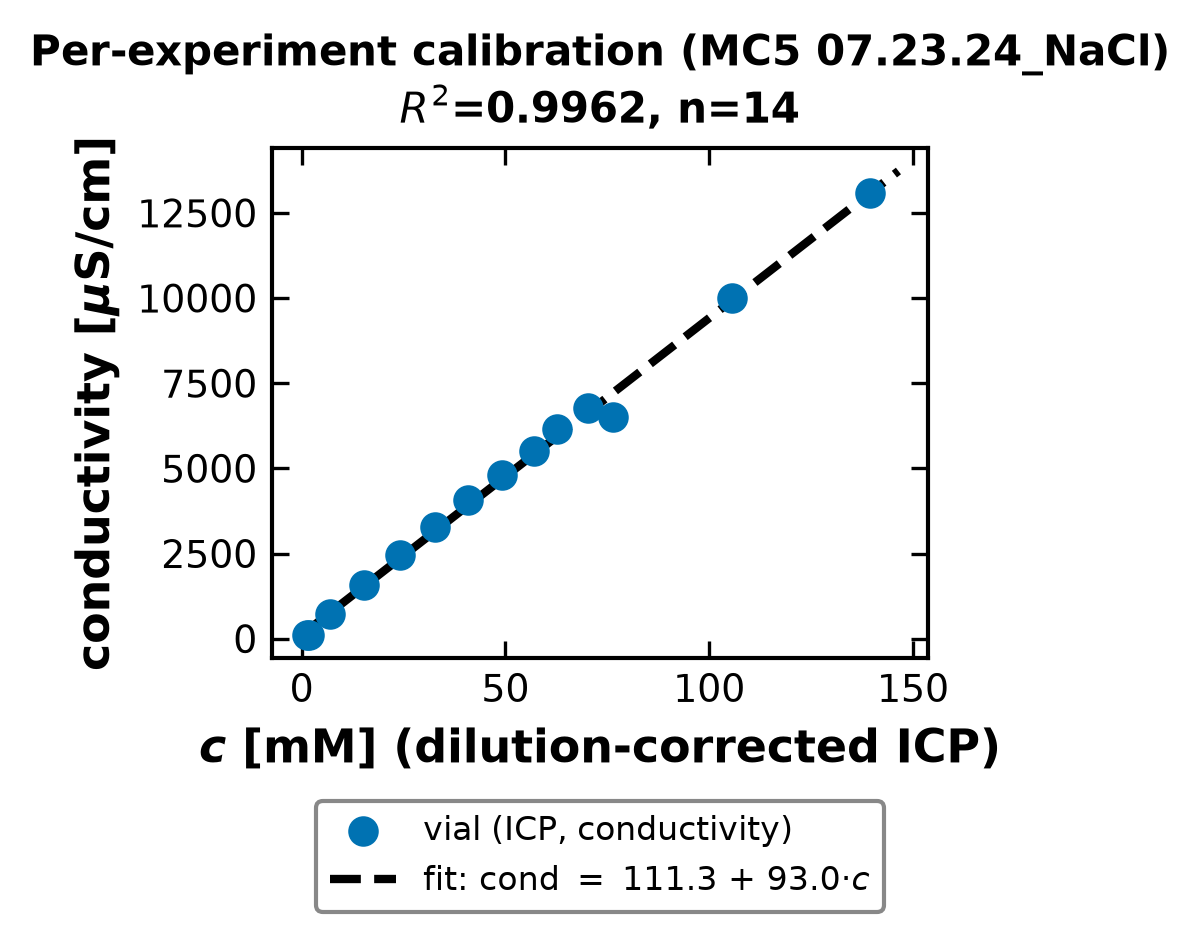
\includegraphics[width=\linewidth]{figures/nacl_preproc_calibration.png}\\{\footnotesize (a) calibration fit}
\end{minipage}\hfill
\begin{minipage}{0.49\textwidth}\centering
  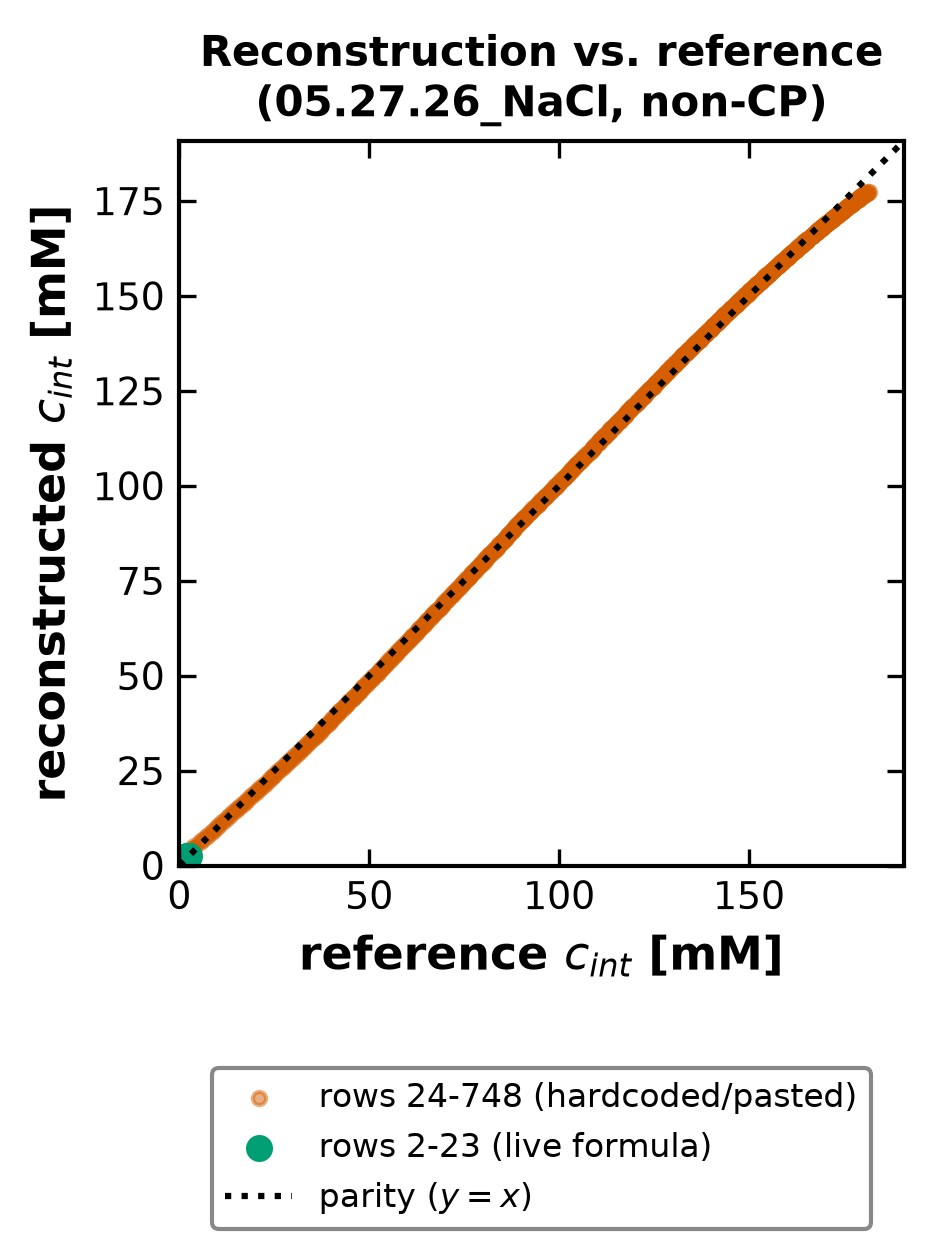
\includegraphics[width=\linewidth]{figures/nacl_preproc_reconstruction.png}\\{\footnotesize (b) reconstruction vs.\ reference}
\end{minipage}
\caption{(a) Per-experiment conductivity calibration (one representative
raw-only run). (b) Parity plot of the reconstructed vs.\ reference $\cint$ for
05.27.26\_NaCl, colored by whether the reference cell is a live formula or a
pasted value.}
\label{fig:preprocvalid}
\end{figure}

\paragraph{Salt generalization.} A single \texttt{Salt}
record (elemental ICP molar mass, cation valence $z$) parametrizes the whole
pipeline for a $1{:}z$ salt (\ce{NaCl} $z=1$, \ce{CaCl2} $z=2$, \ce{LaCl3}
$z=3$; anion always \ce{Cl-}): the ionic-strength multiplier is $\tfrac12
z(z+1)$ and the CP solution diffusivity is $D^{\mathrm s}=(1+z)D_{\text{cation}}
D_{\mathrm{Cl}}/(zD_{\text{cation}}+D_{\mathrm{Cl}})$, both of which collapse to
the familiar \ce{NaCl} forms at $z=1$. ICP-OES measures the elemental metal
(moles metal $=$ moles salt), so the dilution-corrected mg/L$\to$mM conversion
of item~3 below extends unchanged with $M_{\ce{Ca^{2+}}}=\SI{40.08}{g/mol}$,
$M_{\ce{La^{3+}}}=\SI{138.91}{g/mol}$ in place of $M_{\ce{Na+}}$. Resulting
constants: \ce{NaCl} $D^{\mathrm s}=\SI{1.607e-9}{m^2/s}$,
$k=\SI{2.547e-5}{m/s}$; \ce{CaCl2} $D^{\mathrm s}=\SI{1.333e-9}{m^2/s}$,
$k=\SI{2.247e-5}{m/s}$; \ce{LaCl3} $D^{\mathrm s}=\SI{1.301e-9}{m^2/s}$,
$k=\SI{2.211e-5}{m/s}$. Every \ce{CaCl2}/\ce{LaCl3} single-salt dataset (the 3
\ce{CaCl2} runs of \S\ref{sec:cacl2}, the 1 \ce{LaCl3} run of \S\ref{sec:lacl3},
plus the two \ce{NaCl} ``validation twin'' runs) has now been reprocessed from
its raw campaign workbook with CP computed both on and off; full
calibrations, provenance, and CSV inventory in
\texttt{analysis/preprocessing/README.md}. \textbf{The refactor is a strict
generalization}: with no salt argument supplied, every existing \ce{NaCl}
caller reproduces its pre-refactor output byte-for-byte (regression-tested
against all 6 raw-only-run CSVs).

\paragraph{Raw-reprocessing validation (CP-off vs.\ non-CP processed sheets;
CP-on vs.\ the one already-CP-corrected sheet).} \ce{NaCl}'s CP-off
reconstruction reproduces Estrada's/Ouimet's non-CP sheets to $\sim$1\% median
relative error on $\cint$ (as before); the CP-on reconstruction reproduces
the one already-CP-corrected \ce{NaCl} sheet (05.27.26\_NaCl main) to 11.9\%
median (consistent with the pre-existing Validation~2 numbers, confirming the
refactor changed nothing about the \ce{NaCl} CP path). \ce{CaCl2}/\ce{LaCl3}
CP-off reconstruction, however, does \textbf{not} reach the same quality:
median relative error on $\cint$ ranges $1.5$--$23.4\%$ across the three
\ce{CaCl2} runs and is $26.4\%$ for \ce{LaCl3} --- despite \ce{LaCl3}'s
calibration $R^2$ (0.999) being \emph{better} than a typical \ce{NaCl} fit.
Recovering Ouimet's \emph{own} implied calibration from his processed
sheets (his $\cint$ vs.\ his inline retentate conductivity) shows it is in
fact \textbf{linear}: $\kappa=-132.6+152.1\,\cint$ for \ce{CaCl2} MC3 and
$\kappa=-302.6+216.3\,\cint$ for \ce{LaCl3}, both $R^2\approx0.999$ (a
quadratic term barely improves the fit). The discrepancy is therefore
\textbf{not} nonlinearity but a \emph{different calibration}: our vial-ICP fit
($\kappa=+96.4+187.6\,\cint$ for the same \ce{CaCl2} run) differs from
Ouimet's inline calibration in slope ($\sim$20\%) and has an opposite-sign
intercept. The very signature that first suggested nonlinearity --- the
ratio of his $\cint$ to ours shrinking from $\sim$3.1$\times$ at low
concentration to $\sim$1.3$\times$ at high --- is exactly what two
\emph{linear} calibrations with different intercepts produce
(intercept-dominated at low $\cint$; approaching the slope ratio
$187.6/152.1\approx1.23$ at high $\cint$), not a curved relationship. Unlike
\ce{NaCl}, the raw \ce{CaCl2}/\ce{LaCl3} workbooks contain \emph{no} embedded
inline conductivity calibration, so Ouimet's calibration is external to
the data we have and is not reconstructible from raw; no vial-fit convention
(elemental/molecular molar mass, with/without dilution) reproduces it. This is
precisely the vial-vs.-inline instrument question already raised as discussion
point~9 (\S\ref{sec:questions}), now \emph{quantified} as a $20$--$26\%$
concentration effect for the multivalent salts. It is flagged, not silently
accepted (row-level evidence in \texttt{analysis/preprocessing/README.md}).
\S\ref{sec:condmodels} independently confirms this with first-principles
physics: model $\kappa(c)$ (Shedlovsky/MSA) is linear for all three salts
(rebutting an earlier working guess that the gap was nonlinearity), and the
sensor's purely-multiplicative cell constant means Ouimet's large negative
intercepts are physically inadmissible while the vial-ICP fits are close to
the physically expected slope and intercept.
\textbf{Consequence for the CP study:} because the goal is to isolate the
effect of concentration polarization, the \ce{CaCl2}/\ce{LaCl3} CP analysis
applies the CP correction \emph{on top of the processed-sheet bulk}
$\cint$ (the original linear calibration), which both reproduces prior work and
cleanly separates the CP shift from the calibration question; the raw-derived
vial-ICP CSVs are retained as a labeled calibration-sensitivity artifact. The CP
shift itself (median $\%$ change in $\cint$, non-CP$\to$CP) is
\ce{NaCl}~$+10$--$14\%$, \ce{CaCl2}~$+6.6$--$14.9\%$, \ce{LaCl3}~$+28.7\%$ ---
all single-digit-to-tens-of-percent, i.e.\ not negligible for any salt.

\paragraph{Follow-up items (data reduction --- for team discussion).}
\begin{enumerate}[itemsep=2pt]
  \item \note{$A_{\mathrm m}$ and $\rho$ remain \emph{not documented} in the source
    materials; $A_{\mathrm m}\approx\SI{3.95}{cm^2}$ is still \emph{inferred}
    (unchanged from the earlier estimate) rather than confirmed against the
    stirred-cell spec sheet. Still open.}
  \item \note{$\Jw$ smoothing is now a concrete, implemented choice: a
    centered 51-row rolling-window linear-regression slope of $m(t)$, tuned
    by minimizing the error against the one reference $J$ column we have
    (the ``(2)'' sheet) --- median relative error $3.8\%$. This is
    noticeably worse than the near-machine-precision achievable for the
    calibration/derived columns below: $\Jw$ is fundamentally a derivative
    of a noisy signal, so this is a genuine approximation, not a bug, and a
    finer/different smoother could still improve it.}
  \item \note{Conductivity calibration, resolved with one real bug found and
    fixed: the vial block's ``ICP Salt 1 (mg/L)'' is the concentration of
    the \emph{diluted} ICP sample, not the original vial --- it must be
    scaled by the sample/acid dilution factor before converting to mM;
    skipping this understates concentration 40--200$\times$ and gives an
    unphysical calibration slope ($\sim\SI{12000}{\micro S/cm}$ per mM
    instead of $O(100)$). After the fix, per-experiment calibrations fit
    from 6 raw-only NaCl runs' vial (conductivity, ICP) pairs give slopes
    $93$--$\SI{98}{\micro S.cm^{-1}}$/mM ($R^2=0.995$--$0.9995$), consistent
    with each other across 3 membrane cuts and landing within
    $\sim$25\% of the ``(2)'' sheet's embedded formula slope
    ($\SI{76.685}{\micro S.cm^{-1}}$/mM) --- a reasonable cross-probe/session
    agreement. The ICP mg/L$\to$mM conversion uses the \textbf{elemental
    \ce{Na+} molar mass ($\SI{22.99}{g/mol}$)}, confirmed because it (not
    \ce{NaCl}'s $\SI{58.44}{g/mol}$) reproduces each run's stated
    Feed/Diafiltrate concentrations (e.g.\ ``1\,mM Feed, 150\,mM
    Diafiltrate''). \textbf{Caveat:} the two runs already used in
    \S\ref{sec:nacl}/\S\ref{sec:naclAll} (``05.27.26\_NaCl'' and
    ``05.07.24\_NaCl'') turn out to have \emph{no per-vial conductivity
    recorded at all}, so this per-experiment fit could not be independently
    checked against \emph{their} original calibrations --- only against the
    6 newly-processed raw-only runs. \textbf{A further nuance (likely important):}
    the vial-fit line (e.g.\ MC5 07.23.24: $\kappa=111+93\,c$) differs from the
    inline-applicable embedded curve ($\kappa=76.7\,c-64$) not only in slope
    ($\sim$20\%) but in \emph{intercept} ($\sim$+\SI{175}{\micro S/cm}). Because
    this vial-fit calibration is applied to the \emph{inline} retentate/permeate
    conductivity, the intercept offset biases the low-concentration end (where it
    dominates the $\sim$\SI{100}{\micro S/cm} early readings) --- a plausible driver
    of the raw-only runs' reconstruction noise. \emph{Open question for the team:}
    are the vial ``Conductivity @ Temp'' and the inline probe on the same
    instrument/scale? If not, a run's vials should not be used to calibrate its
    inline sensor. Full validation tables:
    \texttt{analysis/preprocessing/README.md}.}
  \item \note{A second, unexpected finding while validating against the
    ``(2)'' sheet: its interfacial-concentration column is a \emph{live}
    calibration formula for only the first 22 of 747 rows; the remaining
    97\% are hardcoded pasted values that do \emph{not} exactly satisfy
    that formula ($R^2=0.999$ against retentate conductivity, but not exact
    -- median 1\% / max 38\% relative deviation). Most of the ``(2)'' sheet
    was therefore produced by some undocumented downstream step, not by the
    formula visible in the cell; \S\ref{sec:nacl}'s fit to that sheet is
    still valid as a fit to whatever values are actually in the column, but
    the column is not as simply reproducible/auditable as the visible
    formula suggests.}
  \item \note{\textbf{Concentration polarization: now implemented for every
    single-salt dataset, and now the primary results-level convention
    throughout.} CP is computed in this preprocessing layer (both on and off)
    for all \ce{NaCl}/\ce{CaCl2}/\ce{LaCl3} datasets (salt-generalization
    paragraph above); the main processed sheet applies the thin-film CP
    correction, the ``(2)'' sheet does not (bulk $=$ interfacial), and
    \textbf{the results in
    \S\ref{sec:nacl}/\S\ref{sec:naclAll}/\S\ref{sec:cacl2}/\S\ref{sec:lacl3}
    (and the AR(1) and raw-measurement work that build on the \ce{NaCl} fit,
    \S\ref{sec:naclAR1}/\S\ref{sec:altform}) are now CP-corrected}, with
    non-CP retained alongside for comparison. The shift was not negligible
    ($+10$--$29\%$ median in $\cint$, salt-dependent; raw-reprocessing
    validation paragraph above) --- see discussion point~11,
    \S\ref{sec:questions}, for the resolved outcome.}
  \item \note{Permeate-side smoothing (cols H, O): the flattening
    ($\approx\SI{0.04}{mM}$ for the first $\sim$14--25 rows in the reference
    sheets) now has a plausible physical explanation --- column O (permeate
    conductivity) is itself blank over that same window, consistent with
    sensor dead-volume before permeate first reaches the conductivity cell,
    rather than arbitrary smoothing. We approximate it (floor + rolling
    median) but do not reproduce it exactly.}
\end{enumerate}

\subsection{First-principles conductivity models (Shedlovsky \& MSA)}\label{sec:condmodels}
The preceding paragraph's ``linear calibration, different source'' conclusion for
\ce{CaCl2}/\ce{LaCl3} was reached empirically (comparing two fitted lines). This
subsection puts a first-principles, peer-reviewed number on it, using the two
validated conductivity models from the group's soft-sensor manuscript
\cite{lilonfe2025softsensors}: the \textbf{same three salts} (\ce{NaCl},
\ce{CaCl2}, \ce{LaCl3}), the \textbf{same conductivity sensor} (Innovative Sensor
Technology LFS 1107, the same model as the DATA3 inline probes), co-authored by
Phillip and Dowling. The \textbf{Shedlovsky} model (manuscript Eqs.~4--9; single
salt, validated to $0.1$\,N ionic strength) and the \textbf{mean spherical
approximation (MSA)} (manuscript Eqs.~11--16; validated to 4\,M, and the model
that extends to binary/ternary mixtures, Eqs.~20--23) both reproduce the
manuscript's own measured $\kappa(c)$ to $\text{MAPE}=1.0$--$2.3\%$ against a
probe with $\sim$0.93\% intrinsic precision (manuscript Table~3, Fig.~3). Code is
vendored verbatim (\texttt{analysis/conductivity\_models/conductivity.py}, run
unmodified) with parameters from the manuscript's Tables~1--2; all DATA3-specific
usage (ranges, plotting, linearity/adjudication analysis) is in
\texttt{analysis/conductivity\_models/calibration\_curves.py}. \ce{NaCl}
($\to\SI{180}{mM}=0.18$\,N) and \ce{CaCl2} ($\to\SI{108}{mM}=0.216$\,N) exceed
Shedlovsky's $0.1$\,N validity at the high end of the DATA3 range, so MSA (valid
throughout) is the primary model here; Shedlovsky is reported alongside and
flagged where extrapolated.

\paragraph{Implementation check.} Reproducing the manuscript's Table~3 MAPEs
against its own experimental data
(\texttt{salts-conductivity-modelling/Data/\{NaCl,CaCl2,LaCl3\}.csv}, at
$T=\SI{298.15}{K}$) confirms the vendored code and parameters before drawing any
conclusions: Shedlovsky/MSA MAPE $=0.96\%/1.16\%$ for \ce{NaCl} (manuscript
$1.0\%$ both), $2.21\%/2.27\%$ for \ce{CaCl2} (manuscript $2.2\%/2.3\%$), and
$1.89\%/2.20\%$ for \ce{LaCl3} (manuscript $1.9\%/2.2\%$) --- all within
$0.2$ percentage points of the published values (\ce{NaCl}'s MSA number is the
largest gap, $1.16\%$ vs.\ $1.0\%$, plausibly from the rounded diffusivities in
Table~2 vs.\ the notebook's unrounded values; immaterial to the conclusions
below).

\paragraph{Linearity verdict (rebuts the nonlinearity guess).} Fitting linear and
quadratic $\kappa(c)$ to the MSA/Shedlovsky curves over each salt's DATA3
$\cint$ range ($T=\SI{298.15}{K}$) gives $R^2\ge0.9971$ for the linear fit in
every case (MSA: \ce{NaCl} $0.9994$, \ce{CaCl2} $0.9976$, \ce{LaCl3} $0.9971$),
a small negative quadratic curvature (concave-down, as expected physically), and
a maximum linear-fit deviation of only $2.1$--$4.6\%$ of the $\kappa$ range
(\ce{NaCl} $2.1\%$, \ce{CaCl2} $4.3\%$, \ce{LaCl3} $4.6\%$) --- concentrated at
the range extremes, not a systematic curve. Combined with the manuscript's own
Fig.~3 and Table~3 for these same salts and sensor, this is the definitive,
first-principles rebuttal of the ``nonlinear conductivity--concentration
relationship'' guess (superseded working hypothesis, corrected above): $\kappa(c)$
\textbf{is} linear to good approximation over the full DATA3 range for all three
salts, so the \ce{CaCl2}/\ce{LaCl3} reconstruction gap is not a modeling artifact
of using a linear calibration.

\paragraph{Adjudicating discussion point 9 (calibration source).} The LFS~1107
sensor obeys $\chi=\Phi\cdot(I/V)$ with cell constant $\Phi$ a \emph{purely
multiplicative} scale (manuscript Eq.~3) --- a probe/cell miscalibration is a
slope error with \textbf{no additive offset}, and physical $\kappa(c)\to0$ as
$c\to0$. The MSA linear fit's intercept over each DATA3 range is small and
\textbf{positive} (\ce{NaCl} $+\SI{394}{\micro S/cm}$, \ce{CaCl2}
$+\SI{831}{\micro S/cm}$, \ce{LaCl3} $+\SI{371}{\micro S/cm}$ --- each
$<5\%$ of that salt's $\kappa$ range), exactly the small-positive-intercept
signature a concave-down curve produces when linearized over a high-$c$ window.
Against this physical anchor: the \textbf{processed-sheet inline} calibrations
(Estrada's for \ce{NaCl}, Ouimet's for \ce{CaCl2}/\ce{LaCl3};
\S\ref{sec:preproc} raw-reprocessing validation paragraph) have slopes
$24$--$13$--$23\%$ \emph{below} the MSA-implied slope (\ce{NaCl}, \ce{CaCl2},
\ce{LaCl3} respectively) \emph{and} large \textbf{negative} intercepts
($-63.7$, $-132.6$, $-\SI{302.6}{\micro S/cm}$) --- physically inadmissible for
a purely multiplicative-scale sensor. The \textbf{vial-ICP fits}
(\S\ref{sec:preproc}) are markedly closer to the physical prediction in both
respects: slopes within $8\%$ of MSA (\ce{NaCl} $-7.9\%$, \ce{CaCl2} $+7.1\%$,
\ce{LaCl3} $-7.8\%$) and \textbf{positive} intercepts of the right order of
magnitude ($+111$, $+96$, $+\SI{94}{\micro S/cm}$). \textbf{The physics
therefore supports the vial-ICP calibration over the processed-sheet inline
formula} as
the more physically defensible convention for all three salts, corroborating
(from an independent, first-principles direction) the calibration-source
conclusion already reached empirically above. \textbf{Caveat:} the manuscript
itself reports the models slightly \emph{underpredict} \ce{CaCl2} and (more)
\ce{LaCl3} conductivity by $\sim2\%$ MAPE (dielectric decrement/hydration
effects on multivalent ions), so this is a \emph{shape/linearity/intercept}
argument, not a to-the-percent absolute calibration authority for the
multivalent salts --- it does not, by itself, resolve which slope is exactly
correct, only that the processed-sheet large negative intercepts are not
physically justifiable and the vial-ICP fits are closer on both counts.
Figure~\ref{fig:condmodels} shows the full picture.

\begin{figure}[H]
\centering
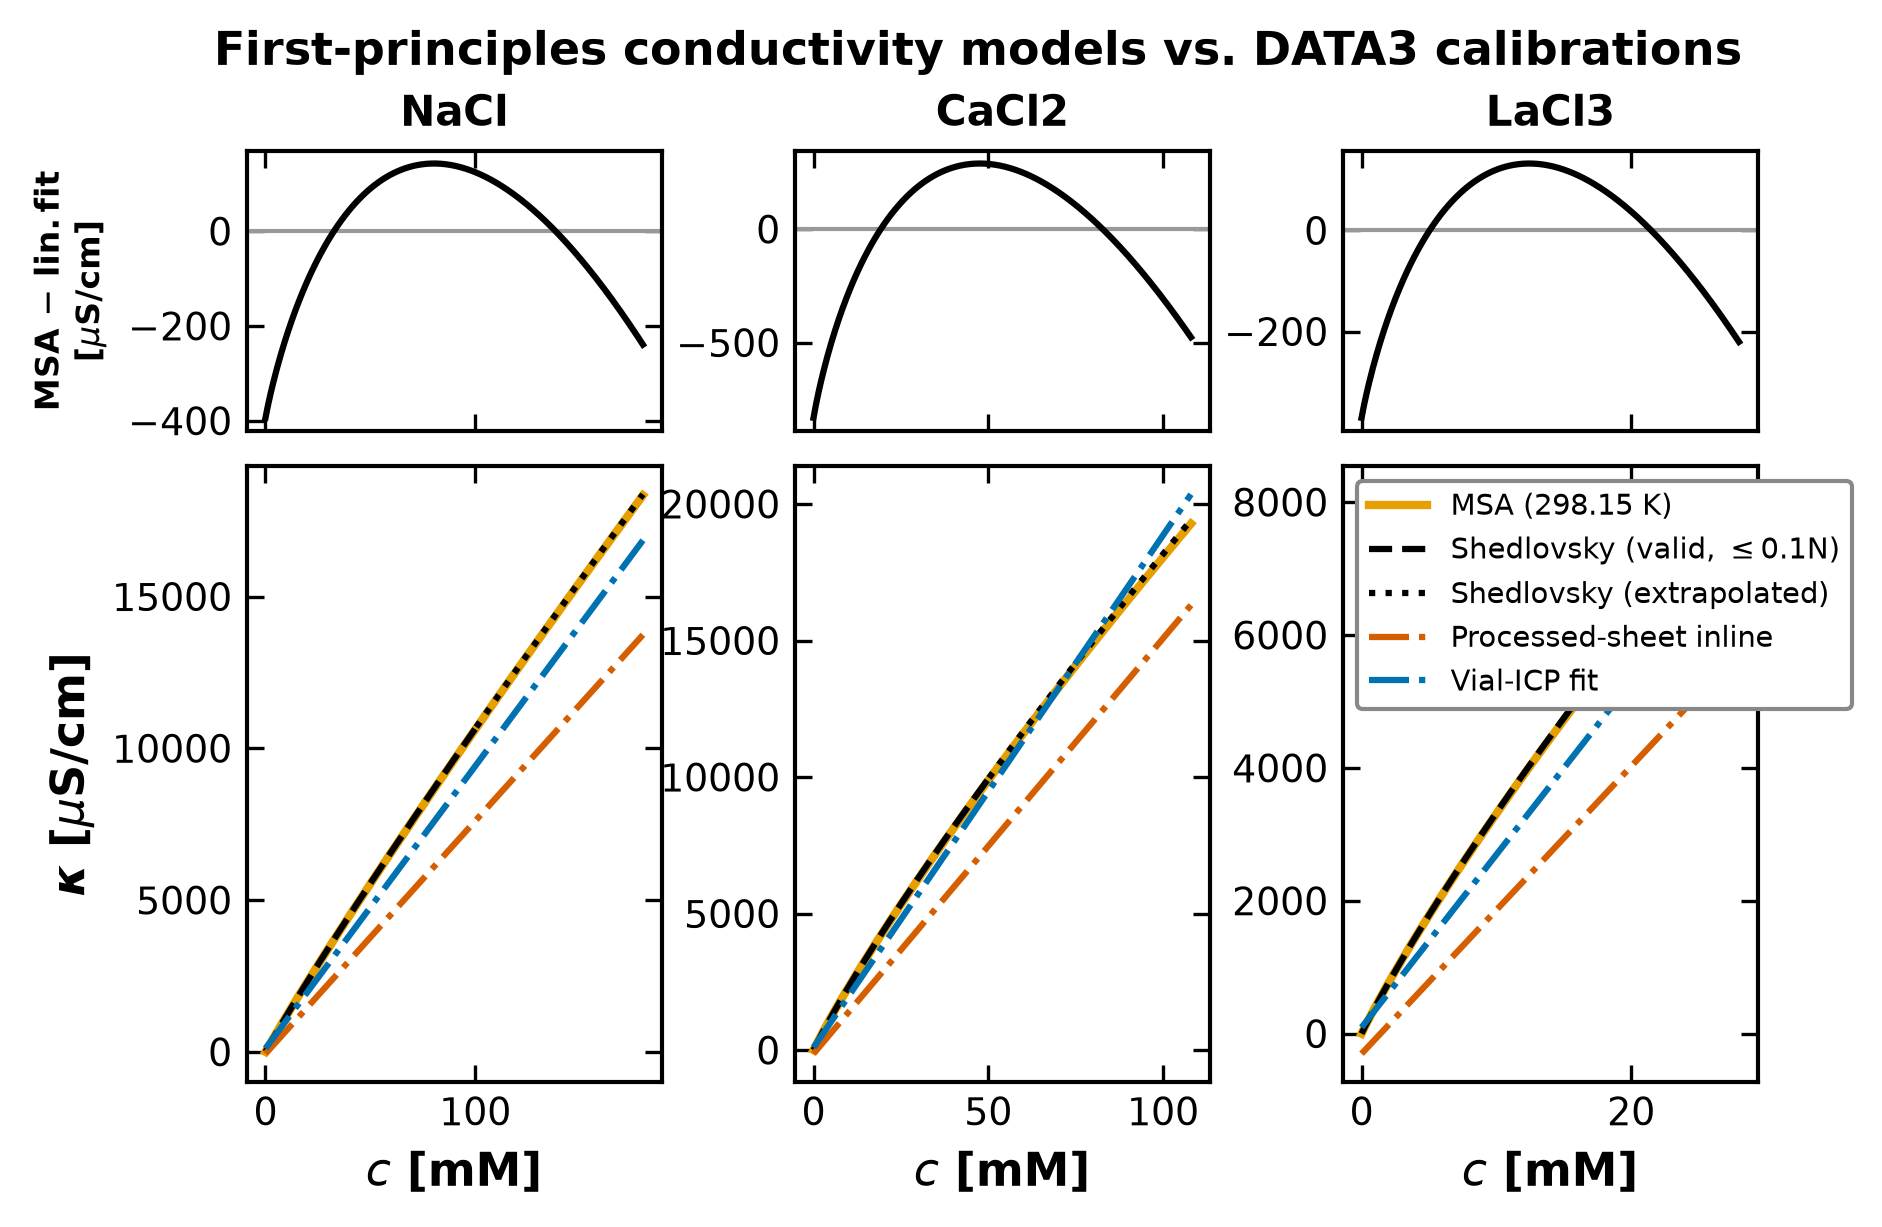
\includegraphics[width=\linewidth]{figures/conductivity_model_calibration.png}
\caption{First-principles \ce{NaCl}/\ce{CaCl2}/\ce{LaCl3} conductivity models
(MSA, primary; Shedlovsky, secondary, dotted where extrapolated beyond
$0.1$\,N) at $T=\SI{298.15}{K}$ over each salt's DATA3 $\cint$ range, with the
processed-sheet inline and vial-ICP linear calibrations overlaid (bottom row) and the
MSA curve's deviation from its own best linear fit (top row, showing the small,
concave-down curvature).}
\label{fig:condmodels}
\end{figure}

\paragraph{Looking ahead: multicomponent conductivity.} The \textbf{MSA
multi-salt model} (manuscript Eqs.~11--16, extended to binary/ternary mixtures
via Eqs.~20--23) is vendored here as a building block for the eventual
multicomponent extension (discussion point~16, \S\ref{sec:questions}): no
new model is needed to go from single-salt to multi-salt conductivity, only
per-ion parameters (already in Table~2) and the additional per-ion ICP
concentrations discussed there. The manuscript's Hunter--Reiner
model-discrimination experimental design (Eqs.~20--23, its Fig.~5) is directly
reusable for planning which multi-salt diafiltration compositions would most
sharply distinguish candidate conductivity models before committing bench time
to them.

\subsection{Donnan partitioning}\label{sec:donnan}
Ion partitioning is set by equal electrochemical potential across the interface
(a common Donnan potential) with membrane electroneutrality including $\chi$; only
the real, positive root is physical, following the group's multicomponent Donnan
exclusion theory \cite{multicompDonnanTheory}. In the ideal limit,
\begin{equation}
  \Big(\tfrac{\cs{1}}{\cm{1}}\Big)^{1/|z_1|}
  =\Big(\tfrac{\cs{2}}{\cm{2}}\Big)^{1/|z_2|}
  =\Big(\tfrac{\cm{3}}{\cs{3}}\Big)^{1/|z_3|}.
  \label{eq:donnaneq}
\end{equation}
Single-salt polynomials appear in two equivalent forms --- the group's partition
coefficient $H$ form, and the membrane-concentration $\cm{}$ form used in the
scanned notes \cite{donnan11notes,donnan21notes,donnan31notes} and Bill's MATLAB
\cite{billmatlab} (divide by $(\cs{})^n$ to convert):
\begin{align}
  \text{$1{:}1$ NaCl, co-ion:}\quad
    &\cm{\co}^2 + |\chi|\,\cm{\co} - \dstar\,\cs{\co}^2 = 0,
    \quad \cm{\co} = \tfrac12\big(-|\chi| + \sqrt{|\chi|^2 + 4\dstar\,\cs{\co}^2}\big),
    \label{eq:11co}\\
  \text{$2{:}1$ \ce{CaCl2}, co-ion:}\quad
    &\cm{\co}^3 + |\chi|\,\cm{\co}^2 - \dstar\,\delta^{\circ}_{\co}\,\cs{\co}^3 = 0,
    \label{eq:21co}\\
  \text{$3{:}1$ \ce{LaCl3}, co-ion:}\quad
    &\cm{\co}^4 + |\chi|\,\cm{\co}^3 - \dstar(\delta^{\circ}_{\co})^2\,\cs{\co}^4 = 0.
    \label{eq:31co}
\end{align}
The $2{:}1$ cubic has a Cardano closed form (denominators $27,729$ for the
co-ion; $216,46656$ for the counter-ion); the $3{:}1$ quartic has no compact
closed form, motivating a nonlinear-constraint treatment (\S\ref{sec:lacl3}).
\note{Confirm the $z\ne1$ non-ideal factors: co-ion carries $\delta^{\circ}_{\co}$
($2{:}1$) and $(\delta^{\circ}_{\co})^2$ ($3{:}1$) beyond $\dstar$.} For mixtures
the SI \cite{siDocx} derives a single polynomial in $H_1=\cm{1}/\cs{1}$ (e.g.\
$H_1^3-\tfrac{|\chi|}{\cs{1}}H_1^2-(1+2\rho)H_1+2\rho=0$ for NaCl+\ce{CaCl2},
$\rho=\cs{2}/\cs{1}$), making the composition dependence of $H$ explicit.

\subsection{Statistical methods}\label{sec:stats}
Let $\boldsymbol\theta$ collect the parameters (here $(|\chi|,\dstar)$),
$y_i$ the response for observation $i$, and $\hat y_i(\boldsymbol\theta)$ the
model prediction. We use the following, in order of increasing rigor. In
plain terms: we first find the single best-fitting $\boldsymbol\theta$, then
ask how uncertain that estimate is by several methods of increasing
computational cost and increasing trustworthiness when the model's response
surface is strongly curved.

\paragraph{Point estimation (nonlinear least squares).} \emph{What it does:}
finds the single parameter vector $\thetahat$ that best fits the data, by
minimizing the total squared mismatch.
\begin{equation}
  \thetahat = \arg\min_{\boldsymbol\theta}\ \SSE(\boldsymbol\theta),
  \qquad
  \SSE(\boldsymbol\theta)=\sum_{i=1}^{n} w_i\big(y_i-\hat y_i(\boldsymbol\theta)\big)^2,
  \label{eq:nls}
\end{equation}
with weights $w_i$ (unity for OLS; inverse measurement variance for the
heteroscedastic WLS used in DATA~2.0 \cite{liu2025data2}, following the same
model-based data-analytics workflow as DATA \cite{ouimet2022data1}). Solved by
trust-region / Levenberg--Marquardt (scipy) or interior point (Ipopt, via
ParmEst).

\paragraph{Linearized (Wald) covariance and intervals.} \emph{What it does
and how to read it:} the simplest error bars --- it approximates the model as
a flat (linear) surface right around the best fit and reports how far
$\boldsymbol\theta$ could move before the fit visibly worsens. Cheap to
compute, but \emph{optimistic} (too narrow) if the true response surface is
noticeably curved near the optimum.
\begin{equation}
  \mathbf V_{\thetahat} = \hat\sigma^2 (\mathbf J^\top\mathbf J)^{-1},
  \quad \hat\sigma^2=\tfrac{\SSE(\thetahat)}{n-p},
  \quad J_{ik}=\tfrac{\partial \hat y_i}{\partial\theta_k}\Big|_{\thetahat},
  \label{eq:cov}
\end{equation}
giving marginal intervals $\hat\theta_k\pm t_{n-p,1-\alpha/2}\sqrt{(\mathbf
V_{\thetahat})_{kk}}$. These assume the model is locally linear in
$\boldsymbol\theta$ (an ellipsoidal region).

\paragraph{Nonlinear (likelihood-ratio / $F$-test) confidence region.}
\emph{What it does and how to read it:} the rigorous version of the Wald
region --- instead of assuming the surface is flat, it directly maps out
every $\boldsymbol\theta$ whose fit is not statistically distinguishable from
the best one, so it can come out curved or lopsided where the model is
nonlinear, rather than a symmetric ellipse. Exact for
Gaussian errors,
\begin{equation}
  \Big\{\boldsymbol\theta:\ \SSE(\boldsymbol\theta)\le
    \SSE(\thetahat)\Big[1+\tfrac{p}{\,n-p\,}\,F_{p,\,n-p,\,1-\alpha}\Big]\Big\},
  \label{eq:ftest}
\end{equation}
equivalently, asymptotically, $\SSE(\thetahat)[1+\chi^2_{p,1-\alpha}/(n-p)]$
(the $\chi^2$ form ParmEst uses). This region can be curved/asymmetric where the
model is nonlinear.

\paragraph{Profile likelihood.} \emph{What it does and how to read it:} the
one-parameter-at-a-time slice through the nonlinear region above --- for each
candidate value of one parameter, it re-optimizes every other parameter and
asks whether the resulting fit is still acceptable, so the reported interval
already accounts for how the parameters trade off against each other. For a
single $\theta_k$, the profile
$\SSE_k(\theta_k)=\min_{\theta_{j\ne k}}\SSE(\boldsymbol\theta)$ yields the
nonlinear interval $\{\theta_k:\SSE_k(\theta_k)\le
\SSE(\thetahat)[1+F_{1,n-p,1-\alpha}/(n-p)]\}$.

\paragraph{Bootstrap.} \emph{What it does:} a model-free resampling check ---
repeatedly draw a new dataset (with replacement) from the observed data,
refit on each, and see how much the resulting estimates scatter. It makes no
assumption about the shape of the response surface, so agreement with the
analytical (Wald/profile) intervals is reassuring, and disagreement flags
that those assumptions may be breaking down. Resample the $n$ cases with
replacement, refit $B$ times,
and take percentile intervals of the resulting $\{\thetahat^{(b)}\}$.

\paragraph{Multi-start optimization.} \emph{What it does:} a convergence
check, not an uncertainty method --- optimize from many initial guesses sampled
over a parameter box; the spread of converged optima diagnoses local minima and
optimizer reliability (used in \S\ref{sec:naclUQ} to explain the MATLAB
convergence issue).

\paragraph{Independence caveat.} All SSE-based intervals above assume independent
errors. Diafiltration data are dense, autocorrelated time series (one run), so
the effective sample size is $\ll n$ and reported intervals are
\emph{optimistic}; this is flagged throughout and is a target of future work.

% ############################################################
\section{Analysis of NaCl data}\label{sec:nacl}
% ############################################################
The analyzed dataset is sheet \texttt{NF270\_MC5 05.27.26\_NaCl (2)} of the
analysis workbook \cite{boeAnalysisWorkbook} (Box \texttt{.../Analyses/BoE
Analysis.xlsx}; repo twin \texttt{data/Rejection\_Analysis.xlsx}); the full
inventory of
available NaCl experiments is in \S\ref{sec:naclAll}.
\note{The ``(2)'' sheet uses \emph{non}-concentration-polarization interfacial
concentrations (bulk $=$ interfacial); see \S\ref{sec:preproc}, follow-up
item~4. This section below reports the CP-corrected refit as primary (with
non-CP retained for comparison), resolving what was earlier an open
decision.}
The Python analysis
(\texttt{analysis/step2\_nacl/}, \texttt{analysis/step3\_nacl\_uncertainty/}) runs
in the documented \texttt{data3-regression} conda environment.

\subsection{Reproduction of the MATLAB analysis}\label{sec:reproMATLAB}
\paragraph{Regression formulation.} Bill's MATLAB
(\texttt{prior\_analysis/\allowbreak{}B\_\allowbreak{}regression\_\allowbreak{}concentration\_\allowbreak{}NAClanal.m}) forms the solute
flux $\Js=\cp\Jw$ and the transformed ``response''
\begin{equation}
  \Delta c_{\mathrm m} \coloneqq \frac{\Js\,\ell}{\Dm},
  \qquad \Dm=\frac{2D_{\text{Na}}D_{\text{Cl}}}{D_{\text{Na}}+D_{\text{Cl}}},\ \ \ell=\SI{80}{nm},
  \label{eq:deltacm}
\end{equation}
then fits the difference of Donnan co-ion roots \eqref{eq:11co}:
\begin{equation}
  f(\boldsymbol\beta;\cint,\cp)=
    \sqrt{\beta_1^2 + 4\beta_2\,\cint^2} - \sqrt{\beta_1^2 + 4\beta_2\,\cp^2},
  \qquad \beta_1 \leftrightarrow |\chi|,\ \beta_2 \leftrightarrow \dstar,
  \label{eq:matlabmodel}
\end{equation}
by nonlinear least squares (guess $\boldsymbol\beta_0=(22.73,0.09)$), with a
brute-force $|\chi|\times\dstar$ residual contour. We ported this to Python/scipy
and reproduced it (Table~\ref{tab:step2}, Fig.~\ref{fig:step2}).

\paragraph{Potential modeling issue (factor of 2).} The Donnan root \eqref{eq:11co}
carries a $\tfrac12$: $\cm{\co,f}-\cm{\co,p}=\tfrac12[\sqrt{\dots\cint\dots}-\sqrt{\dots\cp\dots}]$,
which \eqref{eq:matlabmodel} omits --- so the code fits $2(\cm{\co,f}-\cm{\co,p})$.
Bill notes the MATLAB was preliminary, so we treat the missing $\tfrac12$ as a
bug. It is an \emph{exact reparameterization}: since $f(2\beta_1,4\beta_2)=2f(\beta_1,\beta_2)$
(pull $4$ from each square root), fitting the corrected
$f_{\text{corr}}=\tfrac12 f$ returns the identical SSE surface with $|\chi|$
doubled and $\dstar$ quadrupled (verified: ratios $2.000000$, $4.000000$; SSE
unchanged to machine precision). Fit quality is therefore unaffected; only the
parameter values change. Reassuringly the corrected $|\chi|\approx\SI{50}{mM}$ is
closer to the $\chi\approx\SI{-44}{mM}$ used independently in the BoE
calculations \cite{boeDoc} than the uncorrected $\approx\SI{25}{mM}$ (weak
physical support for the corrected form). \emph{We
adopt the corrected form $f_{\text{corr}}$ as primary hereafter.} \note{$\ell$
and $\Dm$ are held fixed here, but they are \emph{confounded} with $\dstar$
through $B=\Dm H/\ell$ \eqref{eq:Bdef} --- a fixed-vs.-estimated choice
(discussion point~4, \S\ref{sec:questions}) that this section's point estimate
does not resolve.}

\begin{table}[H]
\centering\small
\begin{tabular}{lccccr}
\toprule
Fit & $|\chi|$ [\si{mM}] & $\dstar$ [--] & SSE & $n$ \\
\midrule
MATLAB reproduction (rows 57--748, uncorrected $f$) & $25.18\pm0.14$ & $0.0816\pm0.0001$ & $56.52$ & 692\\
Full valid range (rows 2--748, uncorrected $f$)     & $24.78\pm0.19$ & $0.0813\pm0.0002$ & $129.62$ & 747\\
Corrected (rows 57--748, $f_{\text{corr}}=\tfrac12 f$) & $50.36\pm0.27$ & $0.3263\pm0.0005$ & $56.52$ & 692\\
Corrected (rows 2--748, $f_{\text{corr}}=\tfrac12 f$)  & $49.55\pm0.39$ & $0.3251\pm0.0007$ & $129.62$ & 747\\
\bottomrule
\end{tabular}
\caption{NaCl regression estimates (scipy). The uncorrected rows reproduce Bill's
setup; ``corrected'' restores the $\tfrac12$ of \eqref{eq:11co}. Bill's row
window (57--748) skips the low-concentration startup transient; the full valid
data span rows 2--748.}
\label{tab:step2}
\end{table}

\paragraph{Recommendation for the MATLAB code.} See \S\ref{sec:naclUQ}: switch
\texttt{lsqcurvefit} to \texttt{algorithm=\allowbreak{}'levenberg-\allowbreak{}marquardt'} (its default
trust-region-reflective is prone to boundary-trapping at the $|\chi|\to0$ local
minimum), and restore the $\tfrac12$ in \eqref{eq:matlabmodel}.

\begin{figure}[H]
\centering
\begin{minipage}{0.49\textwidth}\centering
  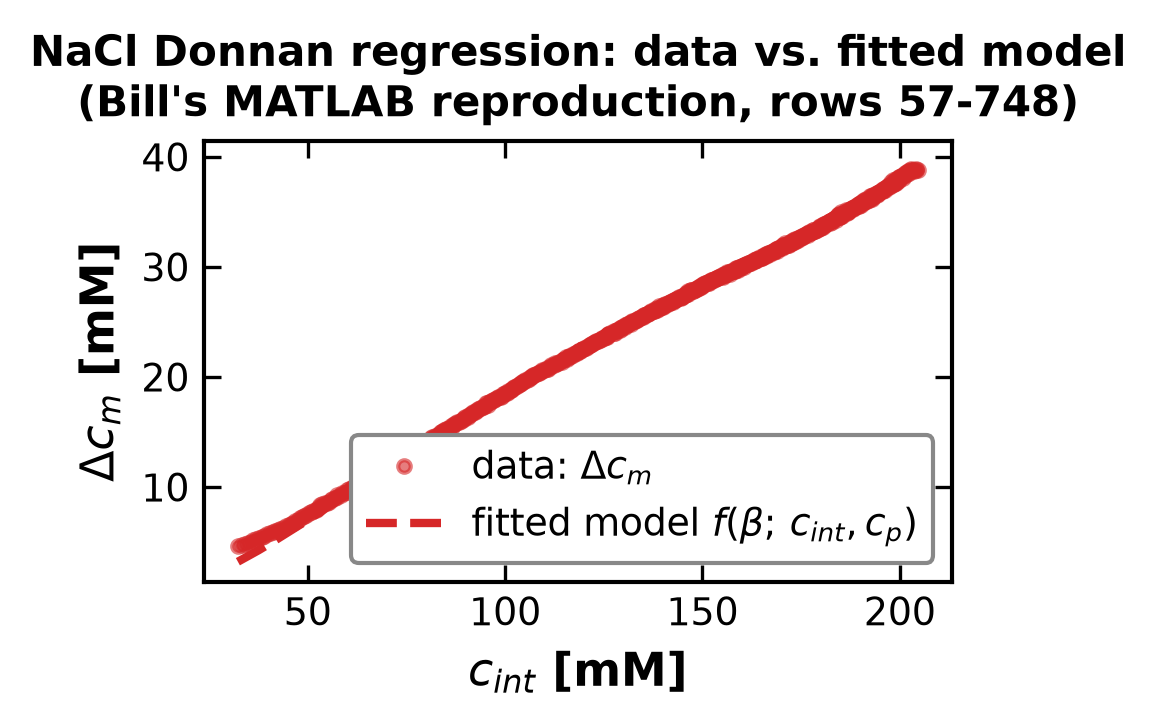
\includegraphics[width=\linewidth]{figures/nacl_fit.png}
\end{minipage}\hfill
\begin{minipage}{0.49\textwidth}\centering
  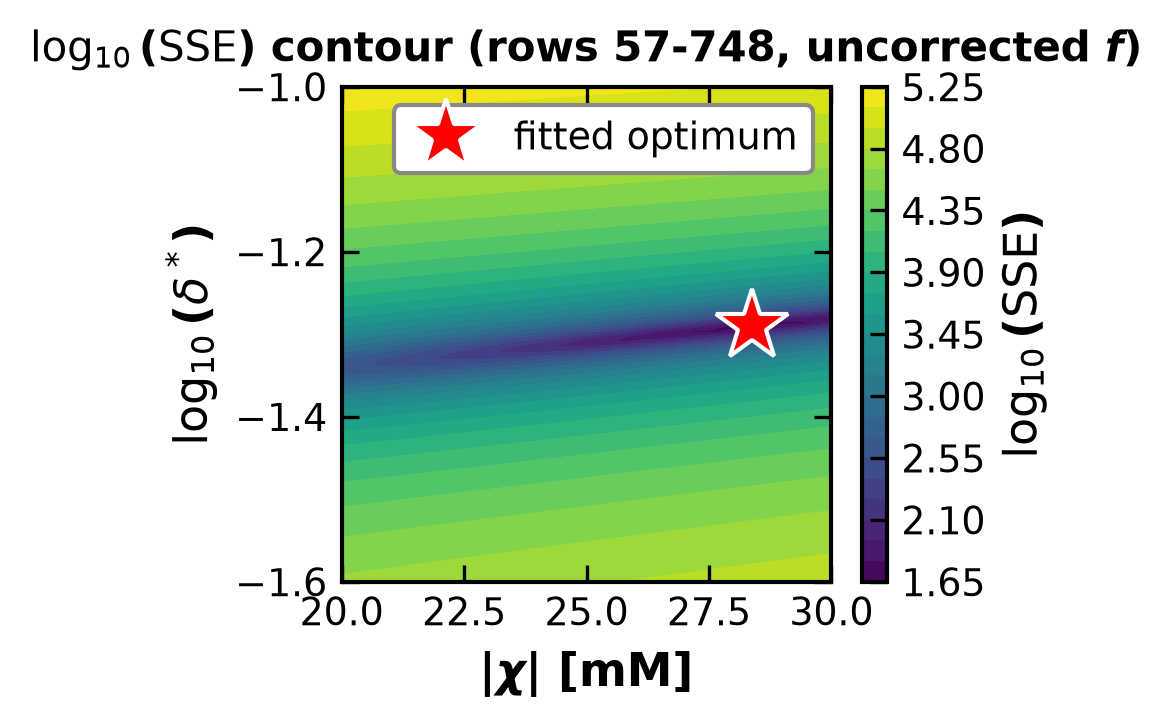
\includegraphics[width=\linewidth]{figures/nacl_residual_contour.png}
\end{minipage}
\caption{Left: fitted model $f$ vs.\ transformed data $\Delta c_{\mathrm m}$
across $\cint\in[25,180]$\,mM. Right: $\log_{10}\SSE$ over the MATLAB grid
($|\chi|\in[20,30]$, $\dstar\in[10^{-1.6},10^{-1}]$) with the optimum marked; the
elongated valley reflects the $|\chi|$--$\dstar$ correlation.}
\label{fig:step2}
\end{figure}

\subsection{Uncertainty analysis and nonlinear confidence regions}\label{sec:naclUQ}
We stress-tested optimizer reliability and quantified uncertainty in both scipy
and Pyomo/ParmEst; the two implementations cross-validate to $6$--$7$ significant
figures.

\paragraph{Concentration polarization is now the primary convention.}
\S\ref{sec:reproMATLAB}'s table reproduces Bill's original (non-CP) MATLAB setup
exactly, on the ``(2)'' sheet's bulk $\cint$. From here on, \textbf{CP is applied
on top of that bulk value} (\S\ref{sec:preproc}, \texttt{analysis/cp\_authors\_bulk.py}:
$\cint^{\mathrm{CP}}=\cp+(\cint^{\mathrm{bulk}}-\cp)\exp(\Jw/k)$, $k_{\ce{NaCl}}=\SI{2.55e-5}{m/s}$,
the same constant used throughout this report) and is the \textbf{standing
convention} for
every table/figure below. Table~\ref{tab:cpvsnoncp} compares: CP shifts
$|\chi|$ from $50.36$ to $\SI{56.74}{mM}$ ($+12.7\%$) and $\dstar$ from $0.3263$
to $0.2049$ ($-37.2\%$, since CP raises $\cint$ enough that $\dstar$ absorbs part
of the shift) --- the \emph{same order of magnitude}, not a change in the
qualitative conclusion that \ce{NaCl} is well-identified with a nonzero fixed
charge of several tens of mM. \S\ref{sec:naclAR1} (AR(1)) and
\S\ref{sec:altform} (raw-measurement) are now also re-run CP-corrected
(discussion point~11, \S\ref{sec:questions}).

\begin{table}[H]
\centering\small
\begin{tabular}{lcccc}
\toprule
& \multicolumn{2}{c}{non-CP (bulk, \S\ref{sec:reproMATLAB})} & \multicolumn{2}{c}{CP-corrected (primary)} \\
Parameter & point est. & 95\% profile CI & point est. & 95\% profile CI \\
\midrule
$|\chi|$ [\si{mM}] & $50.36\pm0.27$ & $(49.68,\,51.04)$ & $56.74\pm0.28$ & $(56.06,\,57.44)$ \\
$\dstar$ [--] & $0.3263\pm0.0005$ & $(0.3250,\,0.3277)$ & $0.2049\pm0.0004$ & $(0.2039,\,0.2059)$ \\
SSE & \multicolumn{2}{c}{$56.52$} & \multicolumn{2}{c}{$52.37$} \\
\bottomrule
\end{tabular}
\caption{\ce{NaCl} CP-vs-non-CP comparison, corrected model, rows 57--748
($n=692$). CP-corrected is now primary; non-CP is retained for comparison and
is what \S\ref{sec:naclAR1}/\S\ref{sec:altform} used before their own
CP-corrected re-run, still shown there alongside the CP-corrected numbers.}
\label{tab:cpvsnoncp}
\end{table}

\paragraph{Convergence diagnosis (why the MATLAB fit was unreliable).}
Across 300 random starts over a deliberately wide box ($|\chi|_0\in[1,200]$\,mM,
$\dstar_0$ log-uniform on $[10^{-3},10]$), scipy \texttt{lm} and \texttt{trf}
reached the global optimum \textbf{100\%} of the time on the CP-corrected data
(as on non-CP); \texttt{dogbox} was trapped \textbf{24.0\%} of the time
(non-CP: $27.3\%$) at a \emph{genuine} local minimum at $|\chi|\to0$, where its
reflective step pins $|\chi|$ to the lower bound. The Jacobian is genuinely ill-conditioned
($\mathrm{cond}(\mathbf J^\top\mathbf J)\sim10^6$--$10^7$; reparameterizing to
$\log_{10}\dstar$ roughly halves it), but conditioning is \emph{not} the cause of
failure --- \texttt{lm}/\texttt{trf} are unbothered by it. ParmEst/Ipopt likewise
hit the global optimum in 100\% of 30 starts. \textbf{Conclusion:} MATLAB
\texttt{lsqcurvefit}'s default \emph{trust-region-reflective} is the analogue of
the failing \texttt{dogbox}; switching to \emph{Levenberg--Marquardt} (or starting
from a physical guess) resolves the unreliability.

\paragraph{Confidence regions and intervals.} At $n=692$ the nonlinear $F$-test
region \eqref{eq:ftest} is visually indistinguishable from the linearized Wald
ellipse --- the NaCl fit is well-identified and nearly linear near the optimum,
CP-corrected as on non-CP. Profile-likelihood intervals are close to Wald
(Table~\ref{tab:ci}), and a 1000-rep case-resampling bootstrap gives SEs close
to Wald ($\mathrm{SE}_{|\chi|}=0.286$ vs.\ $0.277$; $\mathrm{SE}_{\dstar}=0.00039$
vs.\ $0.00040$), all pointing the same direction: Wald is slightly optimistic but
not badly wrong here.

\begin{table}[H]
\centering\small
\begin{tabular}{lccc}
\toprule
Parameter & point est.\ & 95\% profile CI & 95\% Wald CI \\
\midrule
$|\chi|$ [\si{mM}] & $56.74$ & $(56.06,\,57.44)$ & $(56.20,\,57.29)$\\
$\dstar$ [--]      & $0.2049$ & $(0.2039,\,0.2059)$ & $(0.2041,\,0.2057)$\\
\bottomrule
\end{tabular}
\caption{NaCl 95\% confidence intervals, CP-corrected primary result,
corrected model, rows 57--748 ($n=692$). Profile intervals are close to Wald.}
\label{tab:ci}
\end{table}

\paragraph{ParmEst cross-validation.} ParmEst's extensive-form \texttt{theta\_est()}
(each of the 692 rows as one \texttt{Experiment}) matches scipy's estimates to
$\sim$7 significant figures ($|\chi|=56.7424$, $\dstar=0.20489$, $\SSE=52.374$,
CP-corrected) and its \texttt{cov\_est()} Wald SEs to 6 figures; its $\chi^2$ confidence-region
test and bootstrap agree with scipy's $F$-test region and bootstrap. \note{API
notes for us: (i) \texttt{cov\_est()} silently returns $\sim$3.5$\times$ inflated
SEs unless \texttt{measurement\_error} is explicitly \texttt{None}; (ii)
\texttt{calc\_cov}/\texttt{cov\_n} on \texttt{theta\_est()} are deprecated in favor
of \texttt{cov\_est()}; (iii) \texttt{objective\_at\_theta()} re-solves the full
NLP per grid point ($\sim$450\,ms), making fine confidence grids costly.}
\note{Correction: built-in ParmEst multi-start is not yet released -- it is an
open pull request (\href{https://github.com/Pyomo/pyomo/pull/3575}{Pyomo
PR~\#3575}), not a feature of 6.10.1. This session's manual re-initialization
loop (\S\ref{sec:naclUQ}) remains the right approach until that PR merges.}

\paragraph{Key caveat.} All intervals assume i.i.d.\ errors; the 692 points are an
autocorrelated single-run time series, so the true uncertainty is larger than any
figure above. \textbf{This is now corrected}: \S\ref{sec:naclAR1} models the
residuals as an AR(1) process and quantifies how badly the i.i.d.\ regions were
undersized ($n_{\mathrm{eff}}\approx100$ of $n=692$, CP-corrected; both a rigorous
GLS/whitening correction and an effective-sample-size heuristic widen the CIs by
$\sim\!2.5$--$2.7\times$, with the profile still tracking the Wald --- i.e.\ the
correction widens the region but does \emph{not} make it markedly more nonlinear).
Extending the correction to \ce{CaCl2} and richer models
(ARMA / higher-order AR, or explicitly modeling the missing physics --- cf.\
the \ce{CaCl2} residual structure, \S\ref{sec:cacl2}) remain future work.

\begin{figure}[H]
\centering
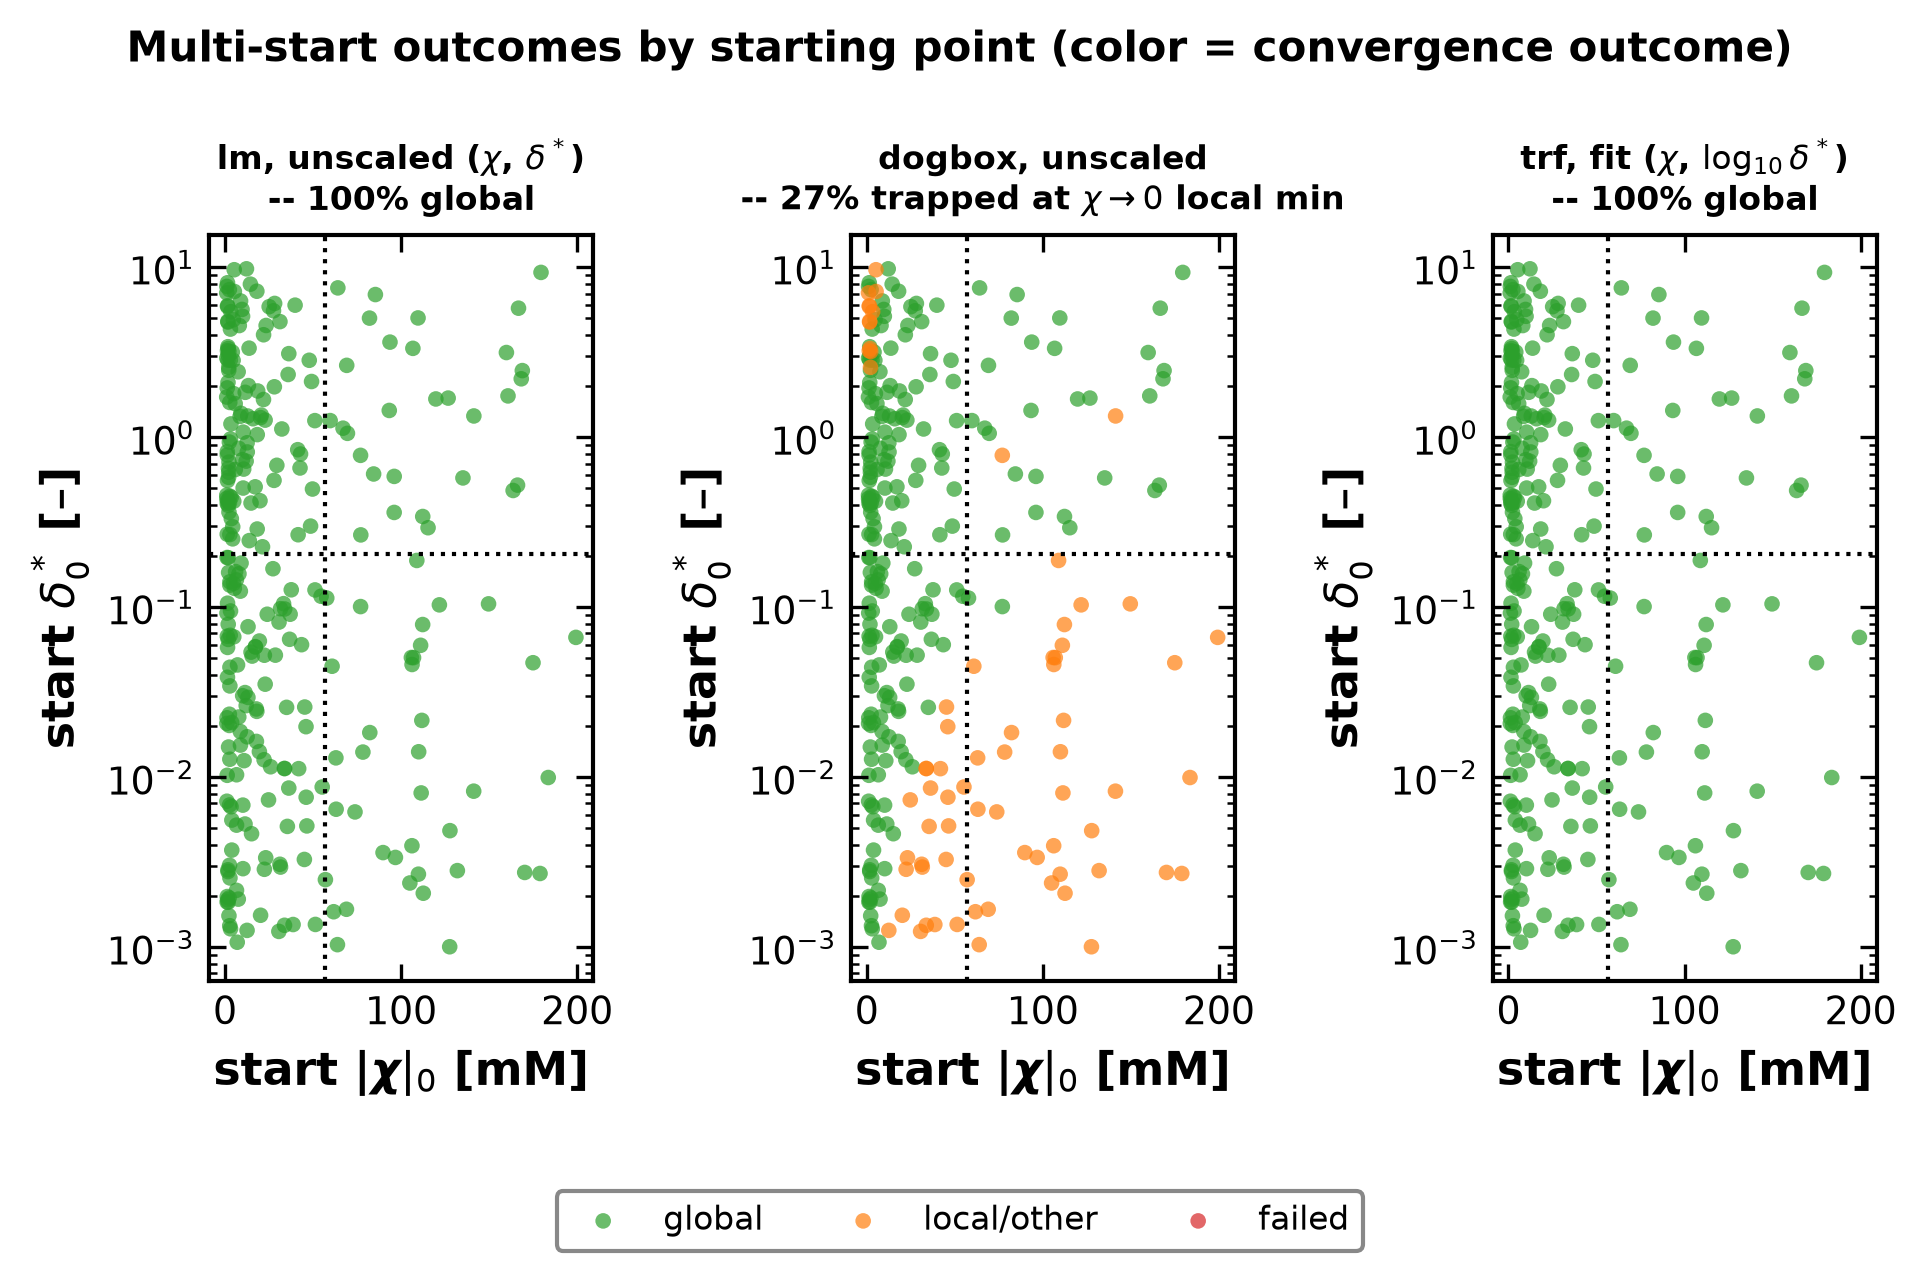
\includegraphics[width=\linewidth]{figures/nacl_multistart.png}\\{\footnotesize (a) scipy multi-start}\\[4pt]
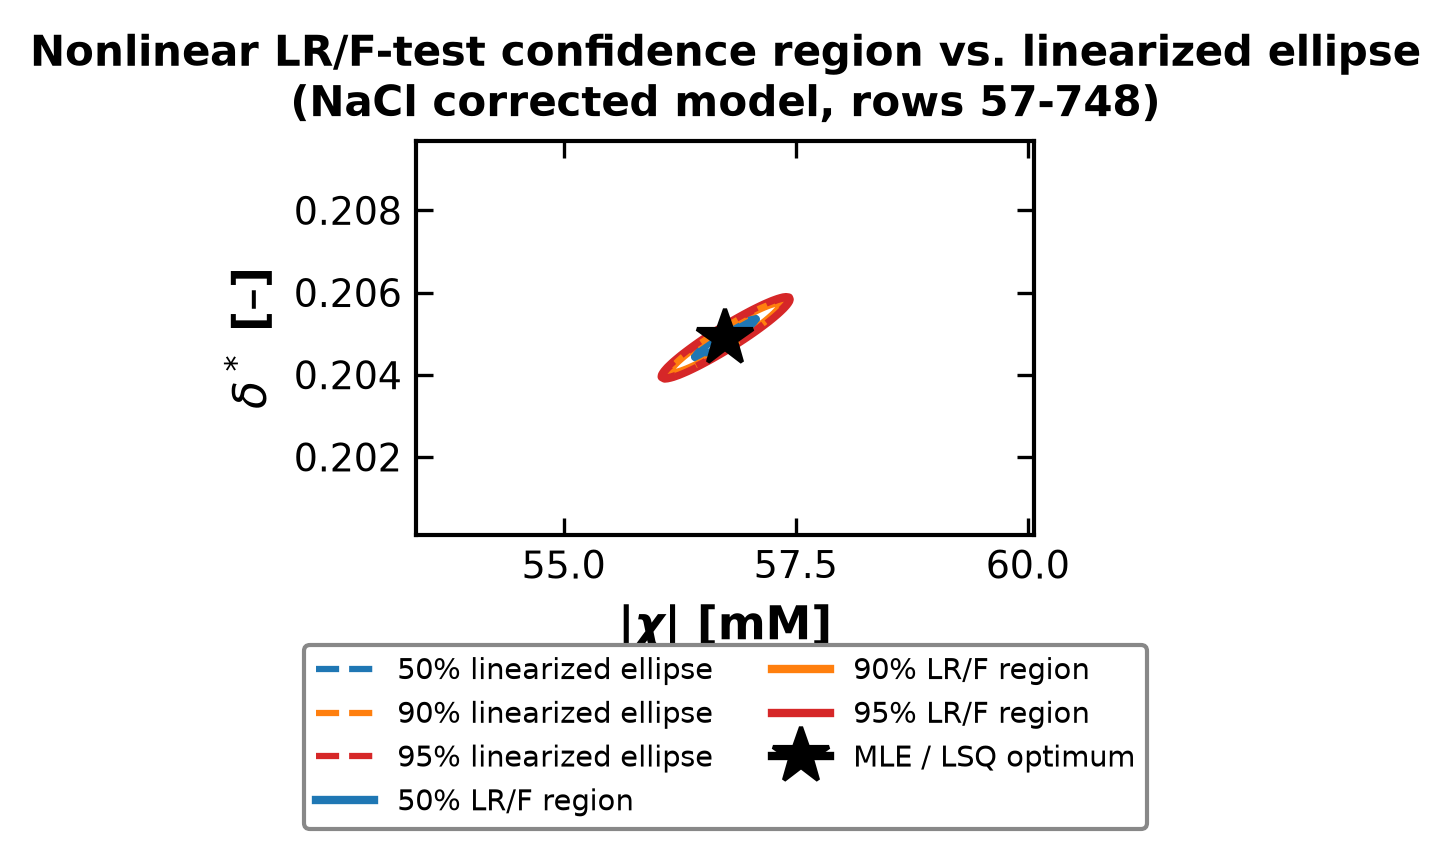
\includegraphics[width=0.49\linewidth]{figures/nacl_confidence_scipy.png}\\{\footnotesize (b) nonlinear region vs.\ ellipse}
\caption{(a) Multi-start convergence (CP-corrected primary data): \texttt{lm}/\texttt{trf}
reach the global optimum from all starts, \texttt{dogbox} is trapped $24\%$ of the time at
$|\chi|\to0$. (b) The nonlinear $F$-test confidence region coincides with the
linearized Wald ellipse at $n=692$. Companion figures
(\texttt{nacl\_profile\_vs\_wald}, \texttt{nacl\_bootstrap\_scipy},
\texttt{nacl\_multistart\_parmest}, \texttt{nacl\_confidence\_parmest},
\texttt{nacl\_bootstrap\_parmest}) are in \texttt{docs/reports/figures/}.}
\label{fig:step3}
\end{figure}

\subsection{Autocorrelation-corrected uncertainty}\label{sec:naclAR1}
The \S\ref{sec:naclUQ} intervals assume i.i.d.\ errors, but the $n=692$ points
are a dense single-run time series, so this section corrects for the
resulting autocorrelation and quantifies how badly the i.i.d.\ regions
understated uncertainty, using the primary NaCl dataset and corrected model
$f_{\text{corr}}$ throughout, \textbf{CP-corrected} (the standing convention,
\S\ref{sec:questions} item~11; non-CP retained alongside for comparison)
(\texttt{analysis/step8\_autocorrelation/ar1\_correction.py}, reusing Step 2/3's
data loading, model, and i.i.d.\ F-test/profile machinery unmodified --
it automatically inherits Step 2's \texttt{APPLY\_CP} default).

\paragraph{AR(1) residual model.} Order the OLS residuals $r_i=y_i-f_{\text{corr}}(\hat{\boldsymbol\theta};x_i)$
by time and model
\begin{equation}
  r_i = \phi\,r_{i-1} + a_i, \qquad a_i\overset{\text{iid}}{\sim}N(0,\sigma_a^2),\ \ |\phi|<1,
  \qquad \hat\phi = \frac{\sum_{i=2}^n r_i r_{i-1}}{\sum_{i=1}^n r_i^2}.
  \label{eq:ar1}
\end{equation}
\paragraph{Effective sample size.}
\begin{equation}
  n_{\mathrm{eff}} = n\,\frac{1-\hat\phi}{1+\hat\phi}, \qquad
  \text{naive CI-inflation} = \sqrt{n/n_{\mathrm{eff}}} = \sqrt{\tfrac{1+\hat\phi}{1-\hat\phi}}.
  \label{eq:neff}
\end{equation}
\paragraph{GLS via Prais--Winsten whitening.} The AR(1) covariance is
$\Sigma_{ij}=\frac{\sigma_a^2}{1-\phi^2}\phi^{|i-j|}$; whitening is the
\emph{linear} operator
\begin{equation}
  \tilde v_1=\sqrt{1-\phi^2}\,v_1, \qquad \tilde v_i = v_i-\phi\,v_{i-1}\ \ (i\ge2),
  \label{eq:whiten}
\end{equation}
applied to any time-ordered sequence $v$. Because \eqref{eq:whiten} is linear,
$\widetilde{(y-f(\boldsymbol\theta))}=\tilde y-\tilde f(\boldsymbol\theta)$ exactly, so the
whitened residual is simply $\tilde r_i(\boldsymbol\theta;\phi)=\widetilde{r(\boldsymbol\theta)}_i$
--- no separate whitening of $y$ and $f$ is needed. \textbf{Cochrane--Orcutt}
iterates $\hat\phi\leftrightarrow\hat{\boldsymbol\theta}$ to convergence: fit
$\boldsymbol\theta$ by OLS, estimate $\hat\phi$ via \eqref{eq:ar1}, refit
$\boldsymbol\theta$ by nonlinear least squares on $\tilde r(\boldsymbol\theta;\hat\phi)$,
re-estimate $\hat\phi$ from the new residuals, and repeat (converged here in 7
iterations, tolerance $10^{-10}$).
\paragraph{Two consistent corrections (not complementary).} Whitening and the
$n_{\mathrm{eff}}$ deflation of \eqref{eq:neff} are \textbf{alternative} ways to
account for the same autocorrelation, not two effects to stack: GLS whitening
already encodes the information loss in the whitened Jacobian
$\tilde{\mathbf J}$, so its region is correctly sized with the \emph{actual}
$n-p$ degrees of freedom; separately, one can skip whitening entirely and
instead deflate $n\to n_{\mathrm{eff}}$ directly in the i.i.d.\ formulas. Using
\emph{both} (whitened SSE \emph{and} $n_{\mathrm{eff}}-p$ df) double-counts the
correction. We therefore report both, side by side, rather than picking one.
\begin{description}
\item[Method A (GLS/whitening).] Wald covariance from the whitened Jacobian,
  $\mathbf V_A=\hat\sigma_a^2(\tilde{\mathbf J}^\top\tilde{\mathbf J})^{-1}$,
  $\hat\sigma_a^2=\SSE_{\text{whitened}}(\hat{\boldsymbol\theta})/(n-p)$; the
  nonlinear $F$-test/profile region on
  $\SSE_{\text{whitened}}(\boldsymbol\theta)=\sum_i\tilde r_i(\boldsymbol\theta;\hat\phi)^2$
  with the \textbf{actual} $n-p$ denominator degrees of freedom.
\item[Method B ($n_{\mathrm{eff}}$ heuristic).] No whitening: keep the OLS fit
  $\hat{\boldsymbol\theta}$ and $\SSE(\boldsymbol\theta)$ from \S\ref{sec:naclUQ}, but
  replace $n$ by $n_{\mathrm{eff}}$ \eqref{eq:neff} everywhere it enters the
  i.i.d.\ formulas:
  \begin{equation}
    \mathrm{SE}_B = \mathrm{SE}_{\text{OLS}}\cdot\sqrt{n/n_{\mathrm{eff}}}, \qquad
    F\text{-test/profile region on }\SSE(\boldsymbol\theta)\text{ with }n_{\mathrm{eff}}-p\text{ df}.
    \label{eq:methodb}
  \end{equation}
\end{description}
\paragraph{Sufficiency of AR(1).} Compare the ACF of the OLS residuals and of
the whitened residuals $\tilde r(\hat{\boldsymbol\theta}_{\text{GLS}};\hat\phi)$
against the $\pm1.96/\sqrt n$ white-noise band; if the whitened ACF falls
inside the band beyond lag 0, AR(1) suffices.

\paragraph{Results (CP-corrected primary fit).} $\hat\phi=0.7430$ (OLS
residuals); Cochrane--Orcutt converges in 7 iterations to $\hat\phi=0.7466$.
This gives $n_{\mathrm{eff}}=100.4$ (\textbf{only $14.5\%$ of $n=692$} are
effectively independent) and a naive inflation factor of $2.63$.
\textbf{The point estimate barely moves}: OLS$\to$GLS (Method A) shifts
$|\chi|$ by $-1.00\%$ and $\dstar$ by $-0.46\%$ ($56.18$ vs.\ $56.74$\,mM;
$0.2039$ vs.\ $0.2049$; Method B does not refit $\boldsymbol\theta$, so its
point estimate is the OLS value by construction) --- the autocorrelation
correction changes the \emph{uncertainty}, not the point estimate.
\textbf{CP vs.\ non-CP:} CP shifts $\hat\phi$ down slightly ($0.7734\to0.7430$
OLS; $0.7758\to0.7466$ Cochrane--Orcutt) and $n_{\mathrm{eff}}$ up slightly
($87.4\to100.4$), narrowing the widening folds from $\sim$2.7--2.9$\times$ to
$\sim$2.5--2.7$\times$ (Table~\ref{tab:ar1ci}) --- \textbf{essentially
unchanged in character}: the autocorrelation is a property of how the dense
time series was collected, not of the CP shift applied to $\cint$, so this
mild narrowing is expected rather than surprising.

\begin{table}[H]
\centering\small
\begin{tabular}{lccccc}
\toprule
Param.\ & point & 95\% Wald (i.i.d.) & 95\% Wald (A) & 95\% Wald (B) & fold A / B \\
\midrule
$|\chi|$ [\si{mM}] & $56.74$ & $(56.20,\,57.29)$ & $(54.80,\,57.55)$ & $(55.32,\,58.17)$ & $2.53\times$ / $2.63\times$ \\
$\dstar$           & $0.2049$ & $(0.2041,\,0.2057)$ & $(0.2020,\,0.2059)$ & $(0.2028,\,0.2069)$ & $2.52\times$ / $2.63\times$ \\
\midrule
Param.\ & point & 95\% profile (i.i.d.) & 95\% profile (A) & 95\% profile (B) & fold A / B \\
\midrule
$|\chi|$ [\si{mM}] & $56.74$ & $(56.06,\,57.44)$ & $(54.46,\,57.94)$ & $(54.92,\,58.62)$ & $2.53\times$ / $2.68\times$ \\
$\dstar$           & $0.2049$ & $(0.2039,\,0.2059)$ & $(0.2015,\,0.2065)$ & $(0.2023,\,0.2076)$ & $2.52\times$ / $2.68\times$ \\
\midrule
\multicolumn{6}{l}{\footnotesize non-CP (pre-CP-correction baseline, retained for comparison), 95\% profile:} \\
$|\chi|$ [\si{mM}] & $50.36$ & $(49.68,\,51.04)$ & $(48.05,\,51.73)$ & $(48.42,\,52.34)$ & $2.71\times$ / $2.89\times$ \\
$\dstar$           & $0.3263$ & $(0.3250,\,0.3277)$ & $(0.3217,\,0.3287)$ & $(0.3226,\,0.3302)$ & $2.70\times$ / $2.89\times$ \\
\bottomrule
\end{tabular}
\caption{NaCl 95\% confidence intervals, i.i.d.\ vs.\ Method A (GLS/whitening,
$n-p$ df) vs.\ Method B ($n_{\mathrm{eff}}$ heuristic), rows 57--748, $n=692$,
CP-corrected primary fit ($n_{\mathrm{eff}}=100.4$); non-CP row for comparison
($n_{\mathrm{eff}}=87.4$). \textbf{Methods A and B agree closely}
($2.5$--$2.7\times$ CP-corrected, $2.7$--$2.9\times$ non-CP, for both Wald and
profile), and \textbf{profile tracks Wald under each method} (profile/Wald
ratio $\approx1.27$ for i.i.d.\ and A, $\approx1.30$ for B, CP-corrected ---
all close to the i.i.d.\ case's own ratio, i.e.\ mild, comparable nonlinearity
throughout, essentially unchanged from non-CP). This confirms the two
corrections are consistent alternatives, and that the region does \emph{not}
become dramatically more nonlinear once the correction is applied without
double-counting.}
\label{tab:ar1ci}
\end{table}

Fig.~\ref{fig:naclar1} (right) shows all three regions are comparable in size
and shape (Method B slightly larger than Method A, both $\sim\!2.5$--$2.7\times$
the i.i.d.\ region, CP-corrected) --- unlike an earlier draft of this analysis, which
combined whitening with the $n_{\mathrm{eff}}-p$ df correction and reported a
spurious $\sim\!8\times$ profile widening with a visibly more elongated
region; that number resulted from double-counting the same correlation twice
and should not be used.
\note{\textbf{Open question for the PI:} Methods A and B are both
defensible and agree closely here, but which should be the report's headline
convention going forward? Separately: is the $n_{\mathrm{eff}}$ heuristic
(Method B) even well justified given AR(1) is not fully sufficient (below) ---
its derivation assumes the AR(1) model is exact, whereas Method A's whitened
residuals still show some structure. Method A (a full GLS refit) is the more
rigorous choice on that basis, but both are reported here rather than
silently picking one.}

\begin{figure}[H]
\centering
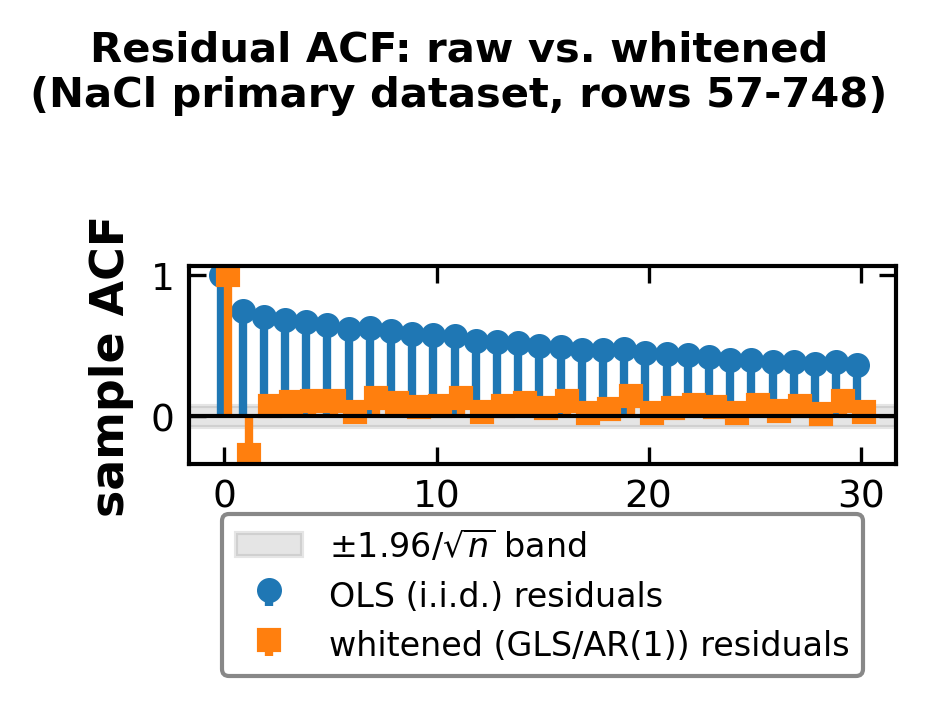
\includegraphics[width=0.49\linewidth]{figures/nacl_ar1_acf.png}\hfill
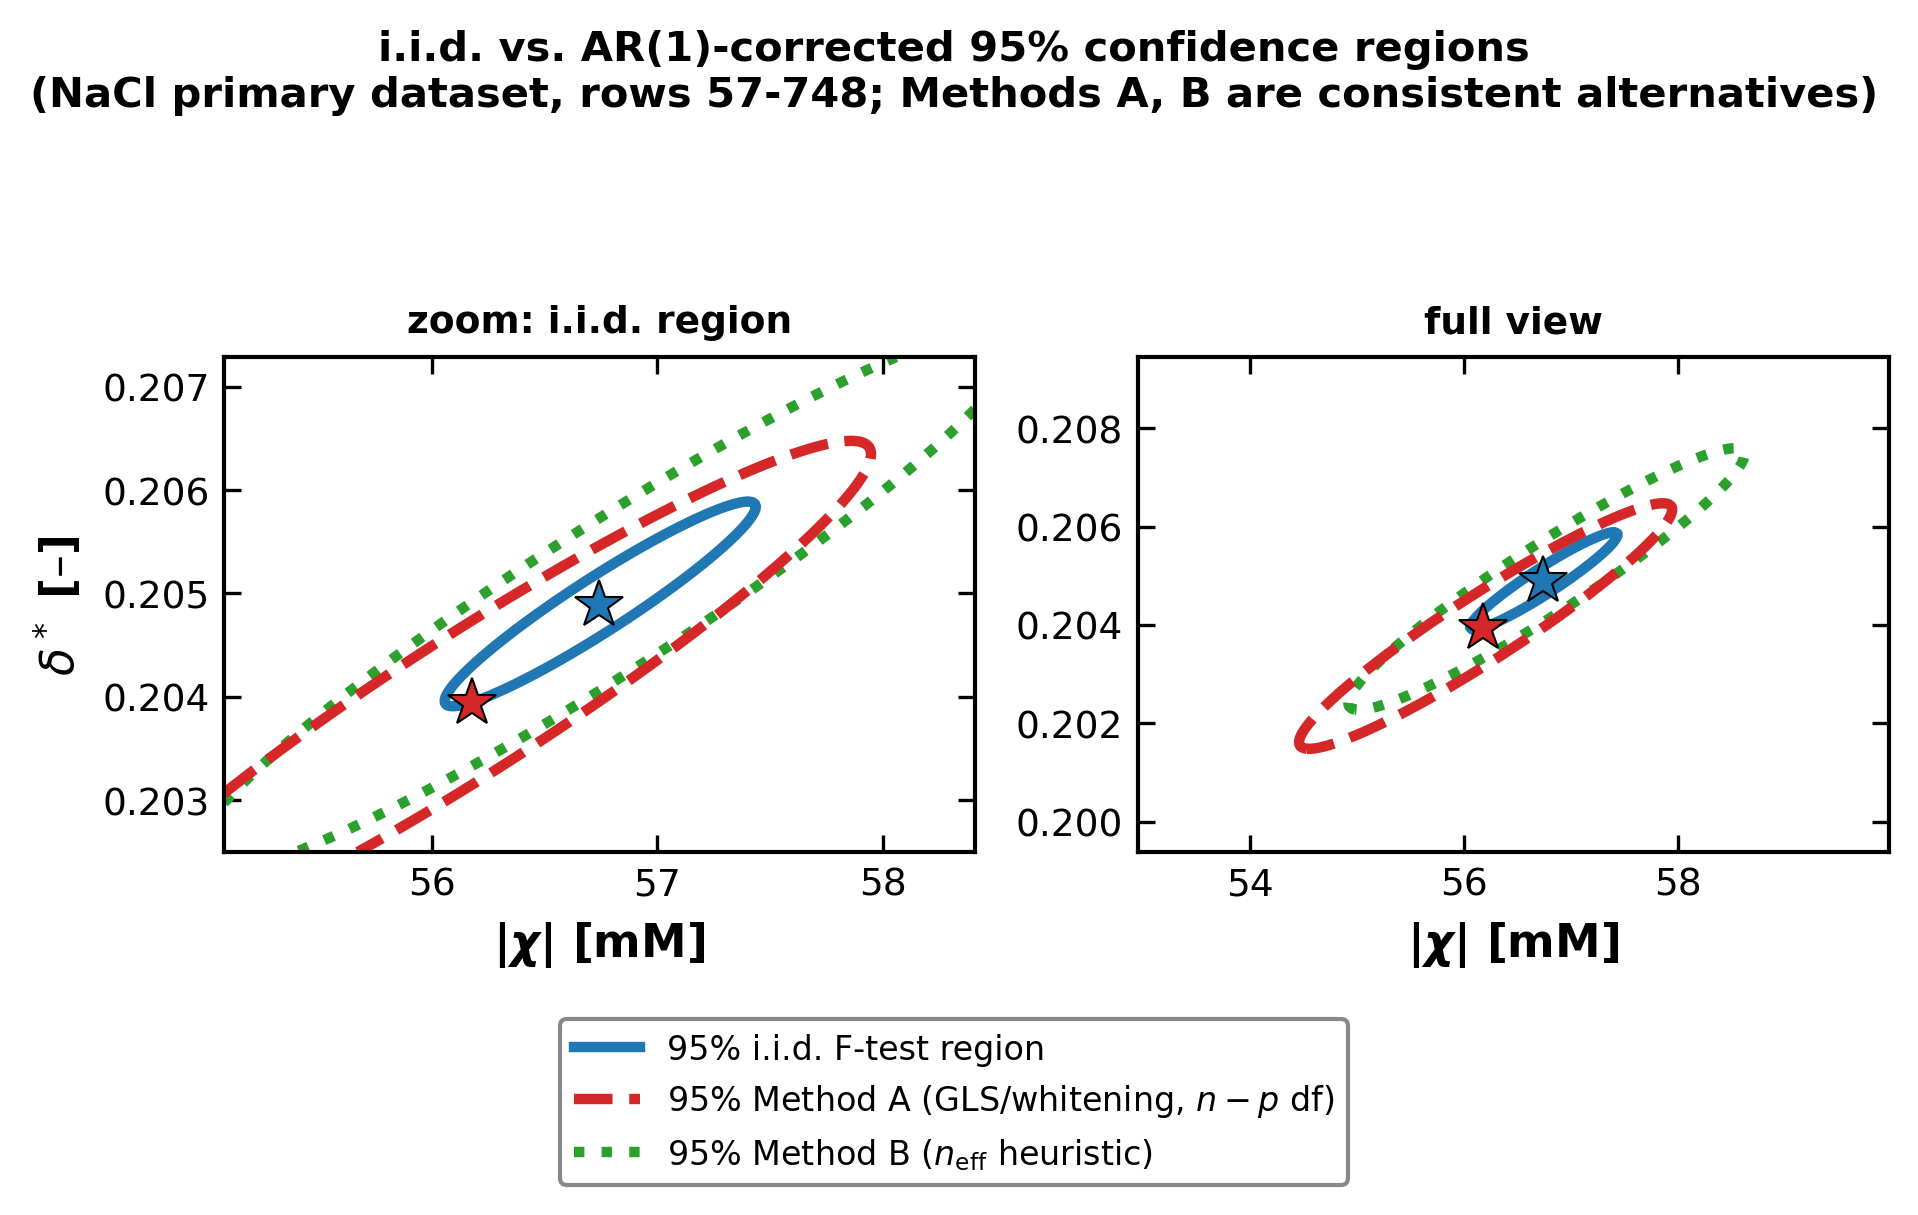
\includegraphics[width=0.49\linewidth]{figures/nacl_ar1_regions.png}
\caption{CP-corrected primary fit. \textbf{Left:} residual ACF, OLS (i.i.d.)
vs.\ whitened (GLS/AR(1)), with the $\pm1.96/\sqrt n$ band. AR(1) removes most
of the raw series' slow decay but $16$ of $30$ lags (including a negative
lag-1 of $-0.28$) still exceed the band --- AR(1) is a large first-order
improvement but not fully sufficient (non-CP: $12$ of $30$, lag-1 $-0.30$,
essentially the same picture); higher-order AR($p$)/ARMA is future work.
\textbf{Right:} the i.i.d.\ vs.\ Method-A vs.\ Method-B 95\% $F$-test regions
on the $(|\chi|,\dstar)$ plane (zoom panel + full view); all three are visible
at comparable scale once the correction is applied consistently (contrast the
double-counted $\sim\!8\times$ region of the earlier draft, which would have
dwarfed this axis).}
\label{fig:naclar1}
\end{figure}

\paragraph{Verdict.} The i.i.d.\ regions understated uncertainty by
$\sim\!2.5$--$2.7\times$ (CP-corrected; $2.7$--$2.9\times$ non-CP), consistently
across both Wald and profile and across both correction methods --- \textbf{this,
not the earlier $\sim\!8\times$ figure, is the number that should be quoted
going forward.} That earlier
number was an artifact of applying the $n_{\mathrm{eff}}-p$ df deflation on
top of the whitened (GLS) SSE surface; whitening and the $n_{\mathrm{eff}}$
heuristic are alternative corrections for the same effect; the earlier draft
combined them and thereby double-counted the correlation. AR(1) captures the
dominant correlation structure and is a necessary correction, but the residual
structure remaining in the whitened ACF (Fig.~\ref{fig:naclar1}, left) shows
it is not fully sufficient; richer models (AR($p$), ARMA, or explicitly
modeling the missing physics, cf.\ the \ce{CaCl2} residual structure,
\S\ref{sec:cacl2}) remain future work, as does extending this correction to
\ce{CaCl2} (the raw time-series reformulation, \S\ref{sec:altform}, is now
also CP-corrected).

\subsection{Alternative formulation: regress on the raw time-series measurements}\label{sec:altform}
The \S\ref{sec:reproMATLAB} fit forms the transformed
$\Delta c_{\mathrm m}=\cp\Jw\ell/\Dm$ and regresses \emph{that} --- so the noisy
\emph{processed} quantities $\cp,\Jw$ appear inside the response, and $\cp$
appears on both sides of the estimation (both as a derived predictor, via the
calibration, and as part of what is predicted). This mis-states the
uncertainty. This section instead poses the regression directly on the
\textbf{raw measured permeate conductivity} $\kappa_p(t)$, with no
transformation of the response, and compares it against
\S\ref{sec:reproMATLAB}--\ref{sec:naclUQ}'s transformed fit
(\texttt{analysis/step9\_raw\_measurement/raw\_regression.py}, reusing the
transformed-fit analysis's data loading, model, and F-test/profile machinery
unmodified).
\note{This is an exploratory \textbf{reduced} forward model on a single raw
channel ($\kappa_p$), not the fully rigorous DATA~2.0-style dynamic DAE /
Soft-Sensor ($\kappa\!\to\!c$ via Shedlovsky/MSA \cite{lilonfe2025softsensors})
treatment of all raw channels jointly (also $\kappa_r$, $m(t)$ as responses,
not just as predictors) --- that remains future work; see the working
assumptions and verdict below.}

\paragraph{Forward model.} Primary dataset: raw sheet \texttt{NF270\_MC5.xlsx
/ 05.27.26\_NaCl} (the raw twin of the ``(2)'' sheet), restricted to the same
row window as \S\ref{sec:reproMATLAB}--\ref{sec:naclAR1} (spreadsheet rows
57--748, $n=692$) for a direct comparison. Known inputs per time $t$:
retentate conductivity $\kappa_r(t)\to$ feed-bulk concentration $c_f(t)$ via
the embedded linear calibration $c=(\kappa-a)/s$ ($a=-63.706$, $s=76.685$,
the same values \S\ref{sec:preproc} uses for this sheet); permeate mass
$m(t)\to\Jw(t)$ via \S\ref{sec:preproc}'s smoothed-slope pipeline (tuned
window $=51$ rows); feed interface $\cint(t)$ is \textbf{CP-corrected}
(the standing convention): the same thin-film model as
\S\ref{sec:preproc}/\S\ref{sec:naclAR1}, $\cint=\cp+(c_f-\cp)\exp(\Jw/k)$,
$k_{\ce{NaCl}}=\SI{2.55e-5}{m/s}$, the same constant used throughout
(\texttt{analysis/cp\_authors\_bulk.py}), permeate unpolarized. The co-ion
mass balance that \emph{defines} $\Delta c_{\mathrm m}$ in \eqref{eq:deltacm}
is, before rearranging into ``$\Delta c_{\mathrm m}$ as the response,'' the
\textbf{implicit equation for $\cp$} at fixed $\boldsymbol\theta=(|\chi|,\dstar)$:
\begin{equation}
  \Jw\,\cp = \frac{\Dm}{\ell}\Big[\cm{\co}(\cint;\boldsymbol\theta) - \cm{\co}(\cp;\boldsymbol\theta)\Big],
  \qquad
  \cm{\co}(c^{\mathrm s};\boldsymbol\theta) = \tfrac12\big(-|\chi|+\sqrt{|\chi|^2+4\dstar (c^{\mathrm s})^2}\big)
  \label{eq:rawimplicit}
\end{equation}
(the Donnan co-ion root, \eqref{eq:11co}). \textbf{The real subtlety}: under
CP, $\cint$ is no longer fixed but itself a function of $\cp$ via the CP
equation above, so $(\cint,\cp)$ must be solved \emph{jointly}. Because the
CP equation is affine in $\cp$ for fixed $(c_f,\Jw,k)$, substituting
$\cint(\cp)$ directly into \eqref{eq:rawimplicit} collapses the $2\times2$
coupled system into a single equation in $\cp$ alone --- an \textbf{exact
reduction}, not an approximation or a seeded/decoupled shortcut. This
reduced equation has a unique root $\cp(\boldsymbol\theta,t)\in[0,c_f]$ for
$|\chi|,\dstar\ge0$ and $\Jw,c_f>0$ (bracketed: at $\cp=0$,
$\cint(0)=c_f\exp(\Jw/k)$ and the left side of \eqref{eq:rawimplicit} minus
the right side is $\le0$; at $\cp=c_f$, $\cint(c_f)=c_f$ regardless of the
exponential factor and the difference is $\Jw c_f>0$ --- the same
Descartes'-rule-style bracketing argument as the non-CP path), solved via a
single \texttt{scipy.optimize.brentq} call per time point (same
computational cost as the non-CP solve; non-CP recovered by setting
$\cint=c_f$ directly, retained for comparison). The predicted measurement is
then $\hat\kappa_p(\boldsymbol\theta,t)=a+s\,\cp(\boldsymbol\theta,t)$ (inverting the
calibration); the residual is $\kappa_p(t)-\hat\kappa_p(\boldsymbol\theta,t)$,
with \textbf{no smoothing or transformation} of the measured $\kappa_p$. At
the converged CP-corrected fit, the CP shift in $\cint$ (relative to $c_f$)
has median $+10.4\%$, max $+28.9\%$ across the 692 time points.

\paragraph{Measurement-error model (working assumption).} No replicate
conductivity measurements exist in this dataset to calibrate
$\sigma_\kappa$ directly, so a generic DATA~2.0-style constant-floor +
proportional-term form is assumed and stated explicitly:
$\sigma_\kappa(\kappa)=\SI{5.0}{\micro S/cm} + 0.01\,|\kappa|$. The weighted
residual $[\kappa_p(t)-\hat\kappa_p(\boldsymbol\theta,t)]/\sigma_\kappa(\kappa_p(t))$
is fit by nonlinear least squares, bounded $|\chi|,\dstar\ge0$ (unlike the
$\Delta c_{\mathrm m}$ \emph{difference} form, the standalone $\cm{\co}$ is not
invariant to the sign of $\chi$, so bounding matters here, as for
\ce{CaCl2}, \S\ref{sec:cacl2impl}). \textbf{Robustness check} (non-CP fit,
not re-run under CP): refitting with uniform (unweighted) residuals gives
$|\chi|=140.3$\,mM, $\dstar=1.114$ --- the same qualitative (large) shift
from the transformed fit persists regardless of the weighting scheme,
confirming this is a genuine effect of the raw-measurement formulation and
not an artifact of the error-model weighting choice. AR(1) correction (where
applied) reuses \S\ref{sec:naclAR1}'s Method A (GLS/whitening, actual $n-p$
df) exclusively.

\paragraph{Results (CP-corrected primary fit).} Table~\ref{tab:rawcompare}
compares the point estimates.
\begin{table}[H]
\centering\small
\begin{tabular}{lcccc}
\toprule
Formulation & $|\chi|$ [\si{mM}] & 95\% profile CI & $\dstar$ & 95\% profile CI \\
\midrule
Transformed (\S\ref{sec:reproMATLAB}) & $56.74$ & $(56.06,\,57.44)$ & $0.2049$ & $(0.2039,\,0.2059)$ \\
Raw measurement (i.i.d.) & $136.39$ & $(133.82,\,139.03)$ & $0.6692$ & $(0.6604,\,0.6783)$ \\
Raw measurement (AR(1)) & $135.73$ & $(125.60,\,146.98)$ & $0.6626$ & $(0.6274,\,0.7015)$ \\
\midrule
\multicolumn{5}{l}{\footnotesize non-CP (pre-CP-correction baseline, retained for comparison):} \\
Transformed (non-CP) & $50.36$ & $(49.68,\,51.04)$ & $0.3263$ & $(0.3250,\,0.3277)$ \\
Raw measurement (non-CP, i.i.d.) & $114.89$ & $(112.25,\,117.60)$ & $1.0143$ & $(0.9994,\,1.0295)$ \\
Raw measurement (non-CP, AR(1)) & $4.92$ & $(1.80,\,60.27)$ & $0.00157$ & $(0.00055,\,0.01155)$ \\
\bottomrule
\end{tabular}
\caption{NaCl point estimates, transformed vs.\ raw-measurement formulation
(rows 57--748, $n=692$), CP-corrected primary rows with the non-CP
pre-CP-correction baseline retained below for comparison. \textbf{The point
estimate shifts
dramatically}: $|\chi|$ more than doubles ($+140\%$ CP-corrected, vs.\
$+128\%$ non-CP), $\dstar$ more than triples ($+227\%$ CP-corrected, vs.\
$+211\%$ non-CP), transformed$\to$raw (i.i.d.) --- \textbf{the CP correction
widens, rather than closes, this gap}. \textbf{Unlike the non-CP case, the
CP-corrected AR(1) row is physically well-behaved} (see verdict below) ---
this is the more notable finding of re-running this analysis CP-corrected.}
\label{tab:rawcompare}
\end{table}

\begin{figure}[H]
\centering
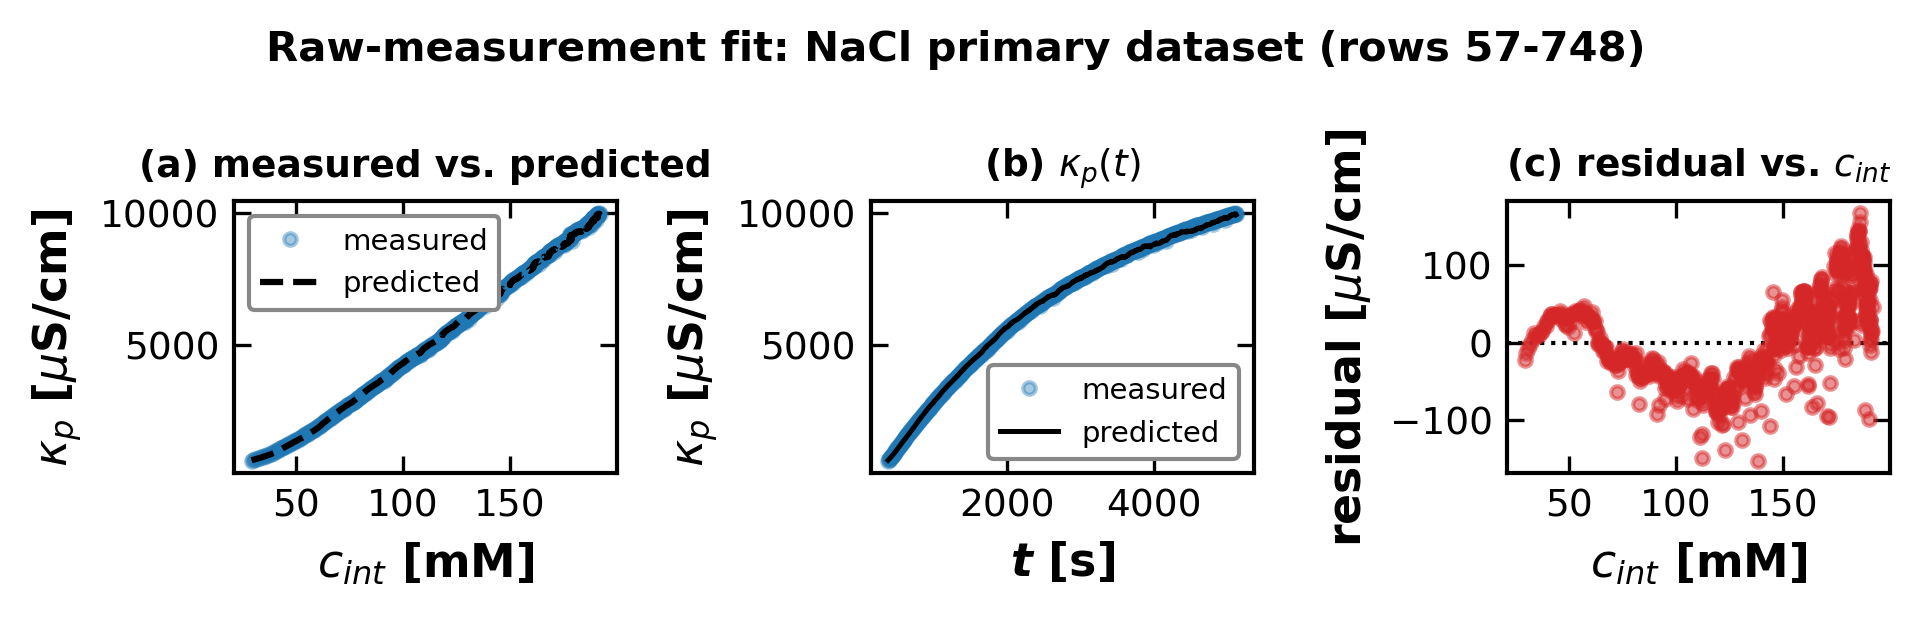
\includegraphics[width=\linewidth]{figures/nacl_raw_fit.png}
\caption{CP-corrected raw-measurement fit (i.i.d.): (a) measured vs.\
predicted $\kappa_p$ vs.\ the solved $\cint$ -- the absolute curve is tracked
closely; (b) $\kappa_p(t)$ time series; (c) residual vs.\ $\cint$, showing
clear systematic wave structure --- the raw conductivity signal carries more
persistent structure than the differenced/transformed response of
\S\ref{sec:reproMATLAB} did, essentially the same picture as the non-CP fit.}
\label{fig:nacluawfit}
\end{figure}

\begin{figure}[H]
\centering
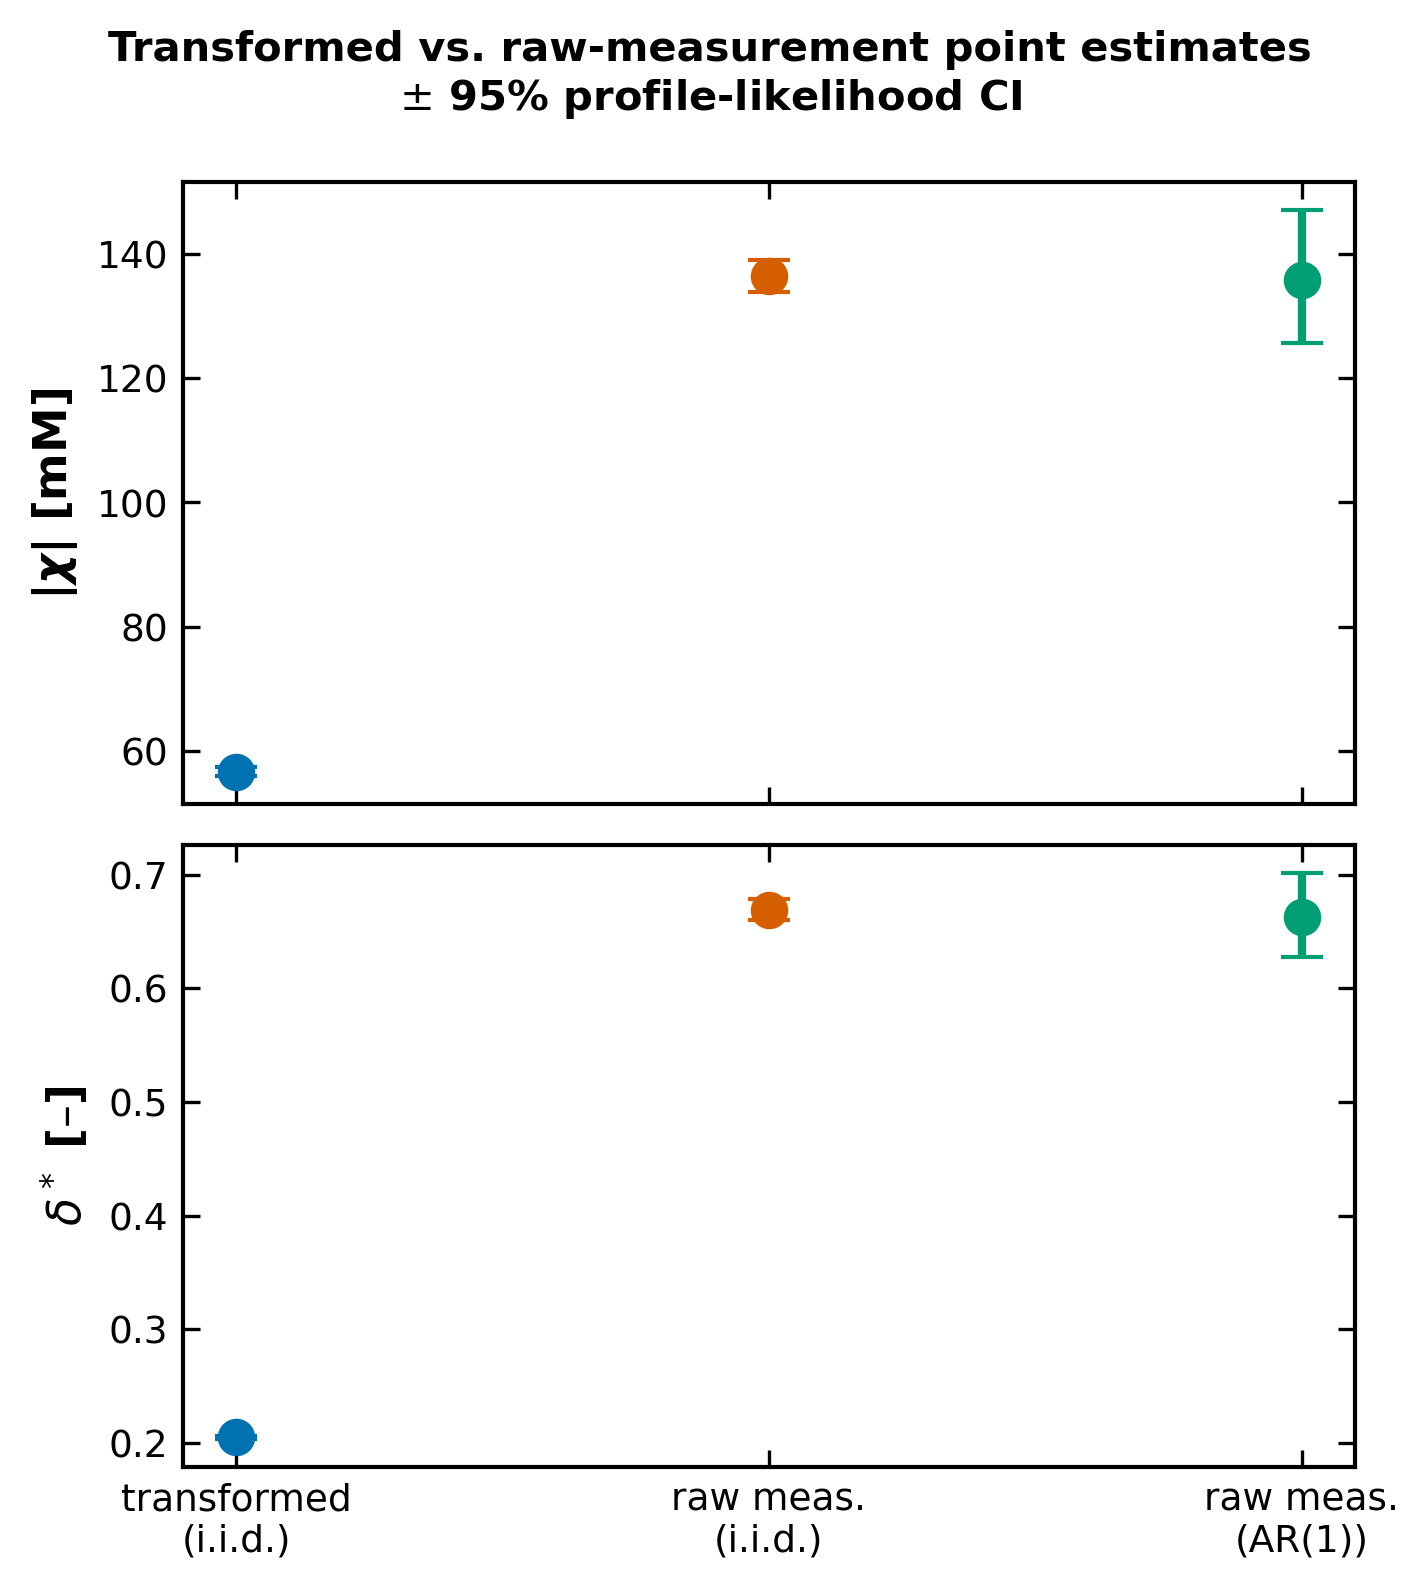
\includegraphics[width=0.7\linewidth]{figures/nacl_raw_compare.png}
\caption{Point estimates $\pm$ 95\% profile-likelihood CI, CP-corrected:
transformed vs.\ raw-measurement (i.i.d.) vs.\ raw-measurement (AR(1)).
Unlike the non-CP version of this figure, the AR(1) panel's error bar is now
of comparable size to the i.i.d.\ one (see verdict) --- the near-unit-root
breakdown does not recur here.}
\label{fig:naclrawcompare}
\end{figure}

\paragraph{Verdict.} \textbf{The errors-in-variables-free formulation moves
the estimates dramatically, and CP widens the gap further}: $|\chi|$ shifts
$+140\%$ transformed$\to$raw (i.i.d.), CP-corrected, vs.\ $+128\%$ non-CP ---
this is a materially different conclusion from \S\ref{sec:reproMATLAB}, not a
minor refinement, and the size of the discrepancy (not just its existence,
nor its direction under CP) is the headline result: it suggests the
transformed fit's $|\chi|\approx\SI{57}{mM}$ may not be robust to the very
errors-in-variables issue this reformulation was designed to test.
\textbf{The surprise: CP substantially, but only partially, resolves
the AR(1) breakdown seen non-CP.} Non-CP, Cochrane--Orcutt drove $\hat\phi$
to the edge of the unit circle ($0.9989$, vs.\ $0.7758$ for the transformed
fit's residuals), collapsing $n_{\mathrm{eff}}$ to $<1$ and producing a
non-physical ``corrected'' CI (Wald interval for $\dstar$ including negative
values; profile CI spanning nearly two orders of magnitude).
\textbf{CP-corrected}, $\hat\phi$ drops to $0.8999$ (Cochrane--Orcutt) and
$n_{\mathrm{eff}}=36.5$ ($5.3\%$ of $n=692$) --- still heavily autocorrelated
and far short of stationary-and-sufficient, but no longer at the unit-root
edge: the Wald/profile CIs are now finite and physically sensible (Wald
$\dstar\in(0.633,\,0.692)$; profile $|\chi|\in(125.6,\,147.0)$,
Table~\ref{tab:rawcompare}), a qualitatively different outcome from the
non-CP near-degenerate result. \textbf{Plausible mechanism} (not
disentangled by this exploratory script): $\cint(t)$'s CP correction is
itself a smooth function of $\Jw(t)$, which drifts slowly over the run;
folding that smooth, physically-motivated nonlinear structure into the
forward model absorbs part of the slowly-varying trend that was previously
left in the residuals as spurious near-unit-root autocorrelation. This does
\emph{not} mean AR(1) is now fully adequate here ($n_{\mathrm{eff}}/n=5.3\%$
is still a severe information loss, well below \S\ref{sec:naclAR1}'s
transformed-fit value of $14.5\%$) --- raw permeate conductivity still rises
smoothly and almost monotonically over the run, more consistent with a
slowly-varying, near-integrated process than a stationary one fluctuating
around a fixed curve, so AR(1) whitening remains an approximation, not a
resolution. Likely remaining contributors: (i) the reduced forward model
still omits time-varying calibration/temperature effects that could explain
part of the residual trend; (ii) the measurement-error model is a working
assumption, uncalibrated against replicate data; (iii) a genuinely richer
noise model (integrated/ARIMA, or a state-space formulation) may still be
needed for raw-signal regression --- consistent with this being, as flagged
above, a reduced model standing in for the fully rigorous DATA~2.0-style
dynamic DAE on all raw channels. \textbf{Recommendation to the group:} treat
this as exploratory, not a corrected replacement for \S\ref{sec:reproMATLAB}
--- CP materially improves the AR(1) diagnostic's behavior but does not
resolve the transformed-vs-raw point-estimate discrepancy (which CP in fact
widens); validate the measurement-error model, add time-varying-calibration/
temperature corrections, and move to a properly stationary or state-space
noise treatment before trusting either the point estimate or its uncertainty
here; extending this comparison to \ce{CaCl2} remains future work.

\subsection{Workflow applied to all available NaCl datasets}\label{sec:naclAll}
We ran the Step-2/Step-3 pipeline across every available single-salt NaCl
experiment (multiple membrane cuts / dates) to test whether $|\chi|$ and $\dstar$
are reproducible across runs and membranes. Table~\ref{tab:nacldata} inventories
the datasets \emph{as they arrived}: three were already processed into the
standard analysis schema (columns B, H, J); six existed only as raw campaign
data and required the raw$\to$processed preprocessing pipeline of
\S\ref{sec:preproc} (interfacial concentration / $\Jw$ / calibration) before they
could be regressed. \textbf{That pipeline has since been built, validated, and
applied to all six raw-only runs --- every row of Table~\ref{tab:nacldata} is now
both processed and regressed}; the last column gives the exact location of each
run's results (\S\ref{sec:naclAllResults} for the summary, the per-dataset
appendix \S\ref{sec:naclappendix} for full detail).

\begin{table}[H]
\centering\footnotesize
\begin{tabular}{ll l r c l}
\toprule
Memb. & Date & Sheet / raw tab & Rows & Arrived as & Now analyzed in \\
\midrule
MC2 & 05.07.24 & \texttt{NF270\_MC2 05.07.24\_NaCl}      & 482  & processed [A] & \S\ref{sec:naclAllResults}, \S\ref{sec:app-mc2} \\
MC5 & 05.27.26 & \texttt{NF270\_MC5 05.27.26\_NaCl}      & 747  & processed [A] & \S\ref{sec:naclAllResults}, \S\ref{sec:app-mc5a} \\
MC5 & 05.27.26 & \texttt{NF270\_MC5 05.27.26\_NaCl (2)}  & 747  & processed [A] & \S\ref{sec:reproMATLAB}--\ref{sec:naclUQ} (\textbf{primary}), \S\ref{sec:app-mc5a2} \\
MC3 & 07.09.24 & \texttt{07.09.24\_NaCl}                 & 404  & raw [Rw]      & \S\ref{sec:naclAllResults} (ill-cond.), \S\ref{sec:app-mc3a} \\
MC3 & 07.22.24 & \texttt{07.22.24\_SNaCl} (diluting)     & 1312 & raw [Rw]      & \S\ref{sec:naclAllResults}, \S\ref{sec:app-mc3b} \\
MC4 & 07.11.24 & \texttt{07.11.24\_SNaCl}                & 423  & raw [Rw]      & \S\ref{sec:naclAllResults}, \S\ref{sec:app-mc4} \\
MC5 & 07.23.24 & \texttt{07.23.24\_NaCl}                 & 516  & raw [Rw]      & \S\ref{sec:naclAllResults}, \S\ref{sec:app-mc5b} \\
MC5 & 07.23.24 & \texttt{07.23.24\_SNaCl}                & 520  & raw [Rw]      & \S\ref{sec:naclAllResults}, \S\ref{sec:app-mc5c} \\
MC5 & 07.23.24 & \texttt{07.23.24\_S2NaCl} (diluting)    & 1324 & raw [Rw]      & \S\ref{sec:naclAllResults}, \S\ref{sec:app-mc5d} \\
\bottomrule
\end{tabular}
\caption{All nine single-salt NaCl diafiltration experiments: \textbf{initial
state} (``arrived as'') vs.\ \textbf{current status} (all nine are now processed
and regressed). \textbf{[A]} = arrived pre-processed in the analysis workbook
\cite{boeAnalysisWorkbook}, Box \texttt{.../Analyses/BoE Analysis.xlsx} (repo twin
\texttt{data/Rejection\_Analysis.xlsx}); the three [A] sheets are identical across
both workbooks. \textbf{[Rw]} = arrived as raw campaign data only, Box
\texttt{.../Diafiltration Campaign and Raw Data/NF270\_MC\{2,3,4,5\}.xlsx}
\cite{rawCampaignMC2,rawCampaignMC3,rawCampaignMC4,rawCampaignMC5} (28-col raw
schema); these six were run through the preprocessing pipeline
(\S\ref{sec:preproc}, \texttt{analysis/preprocessing/}) to obtain $\cint,\cp,\Jw$
before regression. ``Rows'' is each source's declared row count; the row count
actually regressed (after validity filtering) is given per-dataset in
\S\ref{sec:naclAllResults}/\ref{sec:naclappendix}. \emph{Exclude} the mislabeled
tab \texttt{NF270\_MC5 05.26.26\_NaCl} --- its own note identifies it as a
\ce{CaCl2} run. \texttt{S}/\texttt{S2} prefixes denote sequential/reverse
(diluting) runs.}
\label{tab:nacldata}
\end{table}

\subsubsection{Results: all nine datasets}\label{sec:naclAllResults}
\textbf{All nine NaCl runs were regressed} with the corrected model
($f_{\text{corr}}$, full valid range, \textbf{CP-corrected, primary}). The
\textbf{primary CP set is uniformly \emph{our} thin-film CP}: MC2 (Ouimet's
run) and MC5(2) (Estrada's run)
(applied on top of the processed-sheet bulk $\cint$ -- both are the non-CP
convention,
confirmed by the $\cint/\kappa_{\mathrm{ret}}$ coefficient-of-variation
diagnostic, CV$=0.096$ and $0.088$ respectively) and the six newly preprocessed
raw-only runs (reconstructed via \S\ref{sec:preproc}'s pipeline, using the
vial-ICP+CP \texttt{*\_CP.csv} twins). \textbf{MC5-main is the lone
exception}: its column B is already CP-corrected \emph{by Estrada}
(CV$=0.255$, clearly not the non-CP cluster) -- rather than double-applying our
CP on top of hers (which would be wrong), it is kept as an
explicitly-labeled \emph{comparison} row, and \textbf{MC5(2)+our-CP is the
primary ``MC5 (05.27.26)'' entry} in the table, figures, and cross-dataset
comparisons below. Table~\ref{tab:naclall} reports all nine together, marked by
provenance; Figure~\ref{fig:naclall} shows the point estimates and nonlinear
confidence regions (primary datasets only -- MC5-main comparison excluded from
the plots to avoid a confusing second MC5 point), Figure~\ref{fig:naclfits} the
per-dataset fits. \note{The detailed per-dataset appendix,
\S\ref{sec:naclappendix}, still shows the non-CP write-up (predating the
CP-corrected regression re-run) for each
run; refreshing all nine individual write-ups to CP-corrected is flagged as
remaining work, not silently stale.}

\begin{table}[H]
\centering\footnotesize\setlength{\tabcolsep}{4pt}
\begin{tabular}{lclccr}
\toprule
Dataset & $n$ & Provenance & $|\chi|$ [\si{mM}] (95\% CI) & $\dstar$ (95\% CI) & SSE \\
\midrule
MC2 (05.07.24)      & 482  & orig.\ proc.\ (our-CP) & $21.42\ (21.02,\,21.82)$   & $0.1900\ (0.1879,\,0.1921)$ & $2.56$\\
MC5 (05.27.26)      & 747  & orig.\ proc.\ (our-CP, \textbf{primary}) & $56.07\ (55.06,\,57.09)$   & $0.2040\ (0.2026,\,0.2055)$ & $125.04$\\
\emph{MC5 (05.27.26)$^\ddagger$} & \emph{747} & \emph{orig.\ proc.\ (Estrada's CP, \textbf{comparison})} & \emph{$49.56\ (48.58,\,50.55)$} & \emph{$0.3251\ (0.3232,\,0.3270)$} & \emph{$130.07$}\\
MC3 (07.09.24)      & 391  & reconstructed & \multicolumn{2}{c}{\emph{ill-conditioned (diverges)}} & $44192$\\
MC3 (07.22.24, S)   & 1312 & reconstructed & $26.21^\dagger\ (17.96,\,37.89)$   & $0.3025\ (0.2583,\,0.3596)$ & $71798$\\
MC4 (07.11.24, S)   & 317  & reconstructed & $122.23\ (112.67,\,132.73)$ & $1.1768\ (1.1298,\,1.2289)$ & $225.3$\\
MC5 (07.23.24)      & 496  & reconstructed & $74.50\ (72.83,\,76.21)$   & $0.4812\ (0.4753,\,0.4872)$ & $43.8$\\
MC5 (07.23.24, S)   & 500  & reconstructed & $134.79\ (74.14,\,365.73)$ & $0.4001\ (0.2568,\,0.9462)$ & $11734$\\
MC5 (07.23.24, S2)  & 1324 & reconstructed & $77.71\ (53.75,\,121.04)$   & $0.4484\ (0.3451,\,0.6306)$ & $44830$\\
\bottomrule
\end{tabular}
\caption{NaCl regression, \textbf{all nine datasets, CP-corrected (primary)},
corrected model, full valid range; 95\% CIs are profile-likelihood. ``orig.\
proc.'' = arrived pre-processed; the primary CP set (MC2, MC5(2)$\to$``MC5
(05.27.26)'', and the six reconstructed runs) all carry \emph{our} thin-film CP
applied to a non-CP bulk value; the \emph{italicized} row ($\ddagger$: the
``(2)''-suffixed sheet's twin, \texttt{NF270\_MC5 05.27.26\_NaCl} without the
``(2)'') is
Estrada's own already-CP-corrected sheet, kept for comparison only (not
double-CP'd, not part of the primary set/plots). ``reconstructed'' = built from
raw data via \S\ref{sec:preproc}'s
vial-ICP+CP pipeline (a noisier, preliminary tier -- see the
Reconstruction-quality paragraph below). All non-ill-conditioned runs reached the
global optimum in 100\% of multi-starts. $\dagger$MC3~07.22.24's unconstrained fit
converged to the mirror sign ($-26.21$\,mM); harmless since $f_{\text{corr}}$
depends only on $\chi^2$, shown here as $|\chi|$ for consistency with the other
rows.}
\label{tab:naclall}
\end{table}

\paragraph{Reproducibility (originally-processed runs).} \textbf{Our-CP vs.\
Estrada's CP: a third CP-related sensitivity axis.} MC5(2)+our-CP
($|\chi|=\SI{56.07}{mM}$) and MC5-main's own CP (Estrada's)
($|\chi|=\SI{49.56}{mM}$) disagree by $13\%$ (CIs do not overlap). This is
\emph{not} the non-CP-vs-CP question (point 11) or the calibration-source
question (point 9, \S\ref{sec:condmodels}) -- both MC5 entries already carry
\emph{some} CP correction. It is instead an \textbf{implementation-level
discrepancy}: our Leveque-type thin-film mass-transfer coefficient $k$ almost
certainly differs from whatever CP procedure Estrada used (raw reconstruction
already
found our-CP reproduces Estrada's CP MC5 sheet only to $\sim$12\% median --
consistent with this $\sim$13\% parameter-level gap
via the bulk-based mechanism too). \note{Flagged as a minor open item, not a
correctness bug: the \emph{qualitative} conclusions (\ce{NaCl} well-identified,
$|\chi|$ in the tens of mM) are unaffected either way.} \textbf{MC2, now
correctly CP-corrected (it was mistakenly treated as already-CP in an earlier
pass -- its $\cint/\kappa_{\mathrm{ret}}$ CV of $0.096$ places it firmly
in the non-CP cluster, not MC5-main's $0.255$), still disagrees sharply with
MC5} ($|\chi|=21.4$ vs.\ $56.1$\,mM, non-overlapping CIs; non-CP values were
$18.5$ vs.\ $49.6$\,mM -- CP moves both but does not close the gap). We
attribute this primarily to MC2's much \emph{narrower concentration range}
($\cint\lesssim\SI{44}{mM}$ vs.\ MC5's $\lesssim\SI{182}{mM}$): the Donnan
curvature that identifies $|\chi|$ is weak at low concentration, so MC2 is a
less informative experiment rather than necessarily a different membrane.
\note{Neither cut's CI contains the independent
BoE reference $|\chi|\approx\SI{44}{mM}$; MC5(2)+our-CP is now $\sim$27\% high
(MC5-main, Estrada's CP, is $\sim$13\% high), MC2+our-CP is $\sim$2$\times$
low. Worth discussing whether the discrepancy is concentration-range
identifiability, genuine cut-to-cut variation, or the missing-physics issues that
also affect \ce{CaCl2} (\S\ref{sec:cacl2}).}

\paragraph{Reconstruction quality: the six newly preprocessed raw-only runs.} The
six reconstructed runs (Table~\ref{tab:naclall}, now vial-ICP$+$CP) scatter widely
and do \emph{not} agree even among themselves --- the three \texttt{07.23.24} MC5
runs alone give $|\chi|=75$, $135$, and $78$\,mM --- and one (MC3 07.09.24) is
ill-conditioned (diverges to nonphysical $|\chi|$; excluded from
Fig.~\ref{fig:naclall}, which cannot render a divergent optimum on a finite
axis). \note{This scatter is almost certainly dominated by \emph{reconstruction}
uncertainty, not membrane physics: these runs require the full raw$\to$processed
chain ($\sim$3.8\% $\Jw$ smoothing error, per-experiment calibration, vial-ICP
(not the processed-sheet inline calibration), heuristic permeate handling --- \S\ref{sec:preproc}). The
\texttt{S}/\texttt{S2} reverse (diluting) runs are worst behaved (barely
identified, extreme trim-sensitivity, and a visible high-$\cint$ divergence in
Fig.~\ref{fig:naclfits} -- see the per-dataset appendix,
\S\ref{sec:naclappendix}, for exactly where each fit breaks down -- \emph{the
appendix write-ups are not yet refreshed to these CP-corrected numbers}).}
\textbf{The reliable reproducibility conclusion therefore still rests on the
three originally-processed runs above}; the reconstructed tier does not sharpen
identifiability and is preliminary pending the open preprocessing decisions
(\S\ref{sec:preproc}).

\begin{figure}[H]
\centering
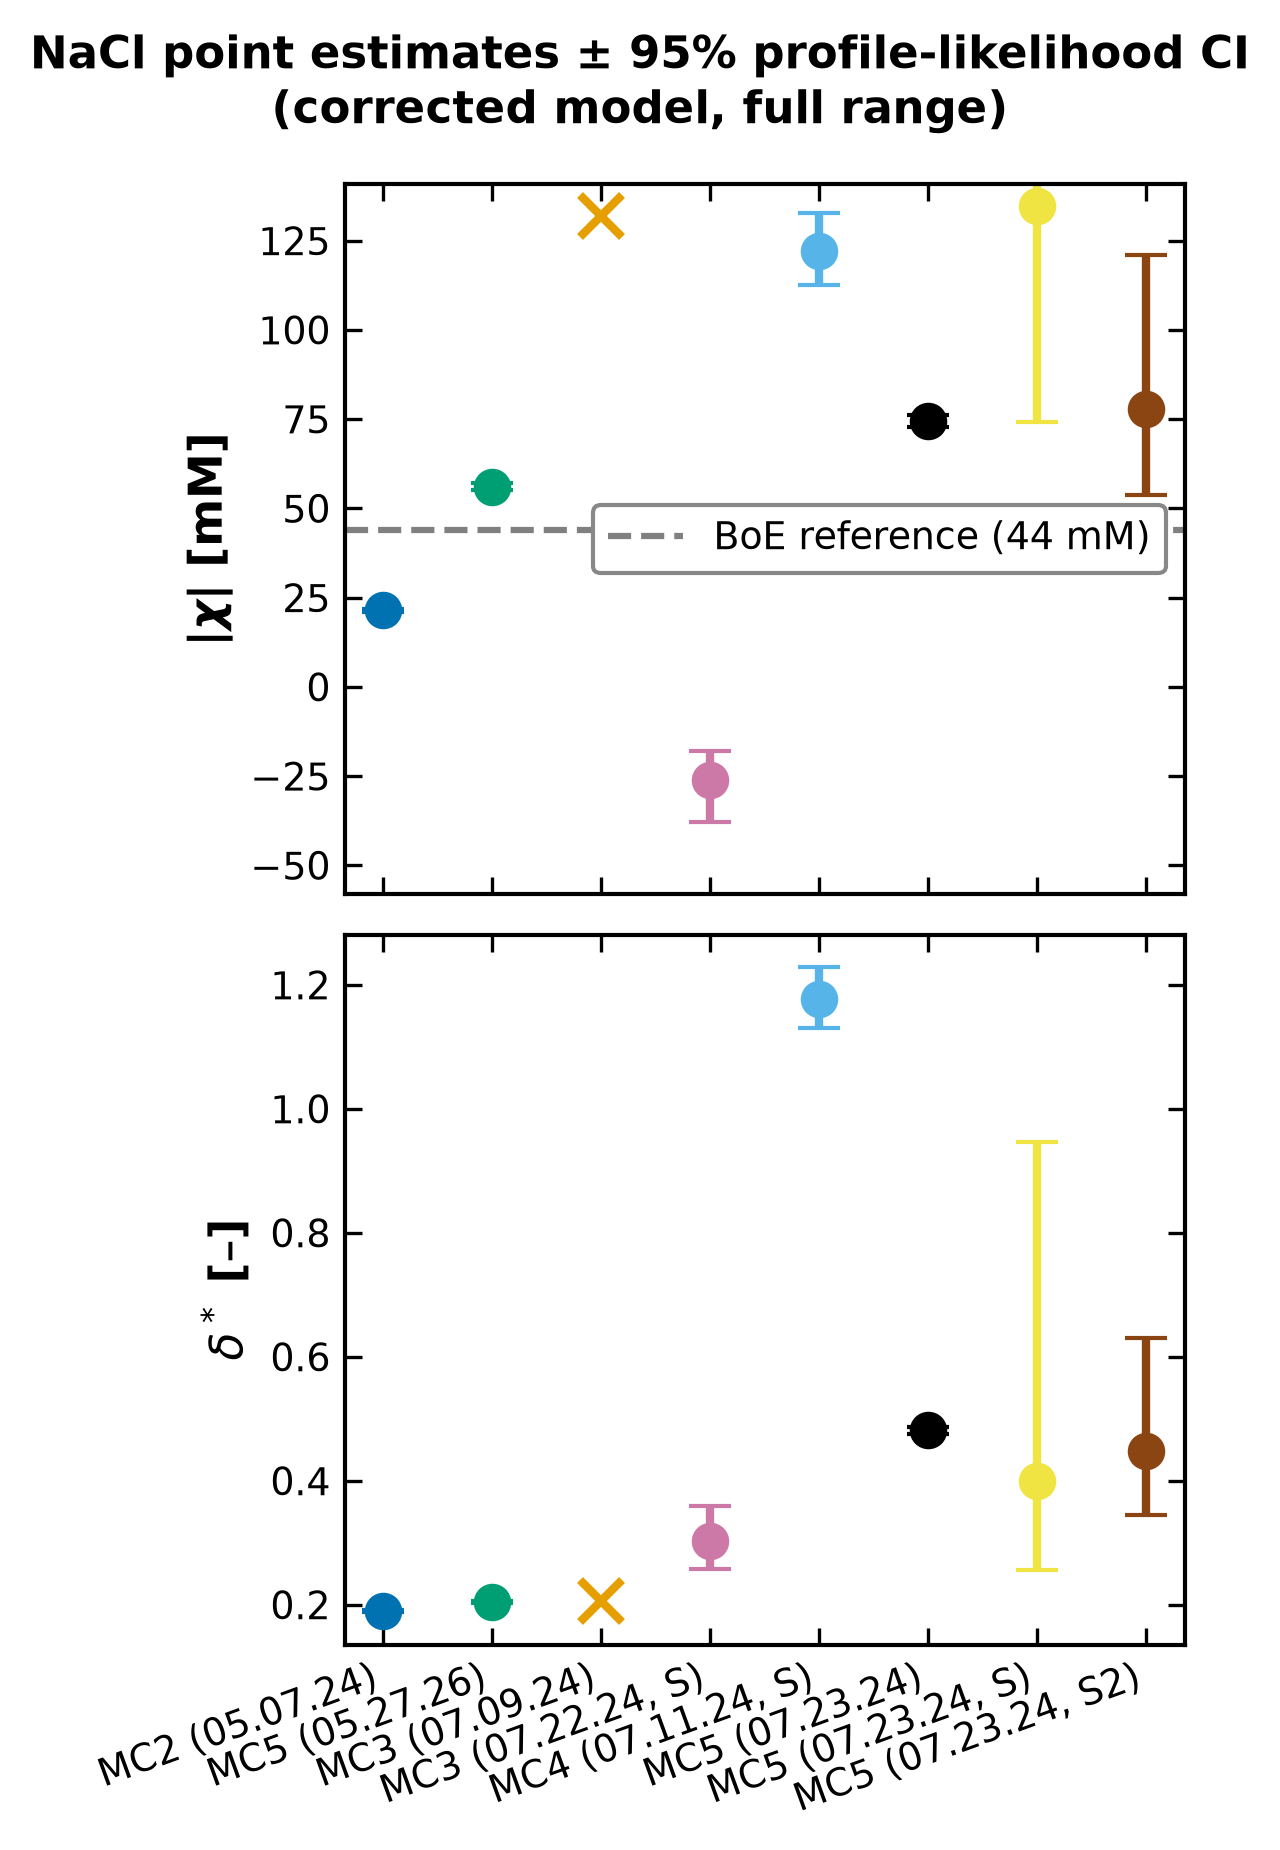
\includegraphics[width=0.6\linewidth]{figures/nacl_all_estimates.png}
\caption{NaCl point estimates $\pm$ 95\% profile-likelihood CI across the eight
\textbf{primary} (uniformly our-CP) datasets (corrected model, full range,
\textbf{CP-corrected}; MC3 07.09.24
omitted -- ill-conditioned, see text; the MC5-main comparison row
(Estrada's CP) is excluded here to avoid a confusing second MC5 point, see
Table~\ref{tab:naclall}). MC3 07.22.24 (S) plots at its raw fitted
value ($-26.21$\,mM, the unconstrained fit's mirror-sign convergence,
Table~\ref{tab:naclall}); read as $|\chi|=26.21$\,mM. Dashed line: BoE reference
$|\chi|\approx\SI{44}{mM}$.}
\label{fig:naclestimates}
\end{figure}

\begin{figure}[H]
\centering
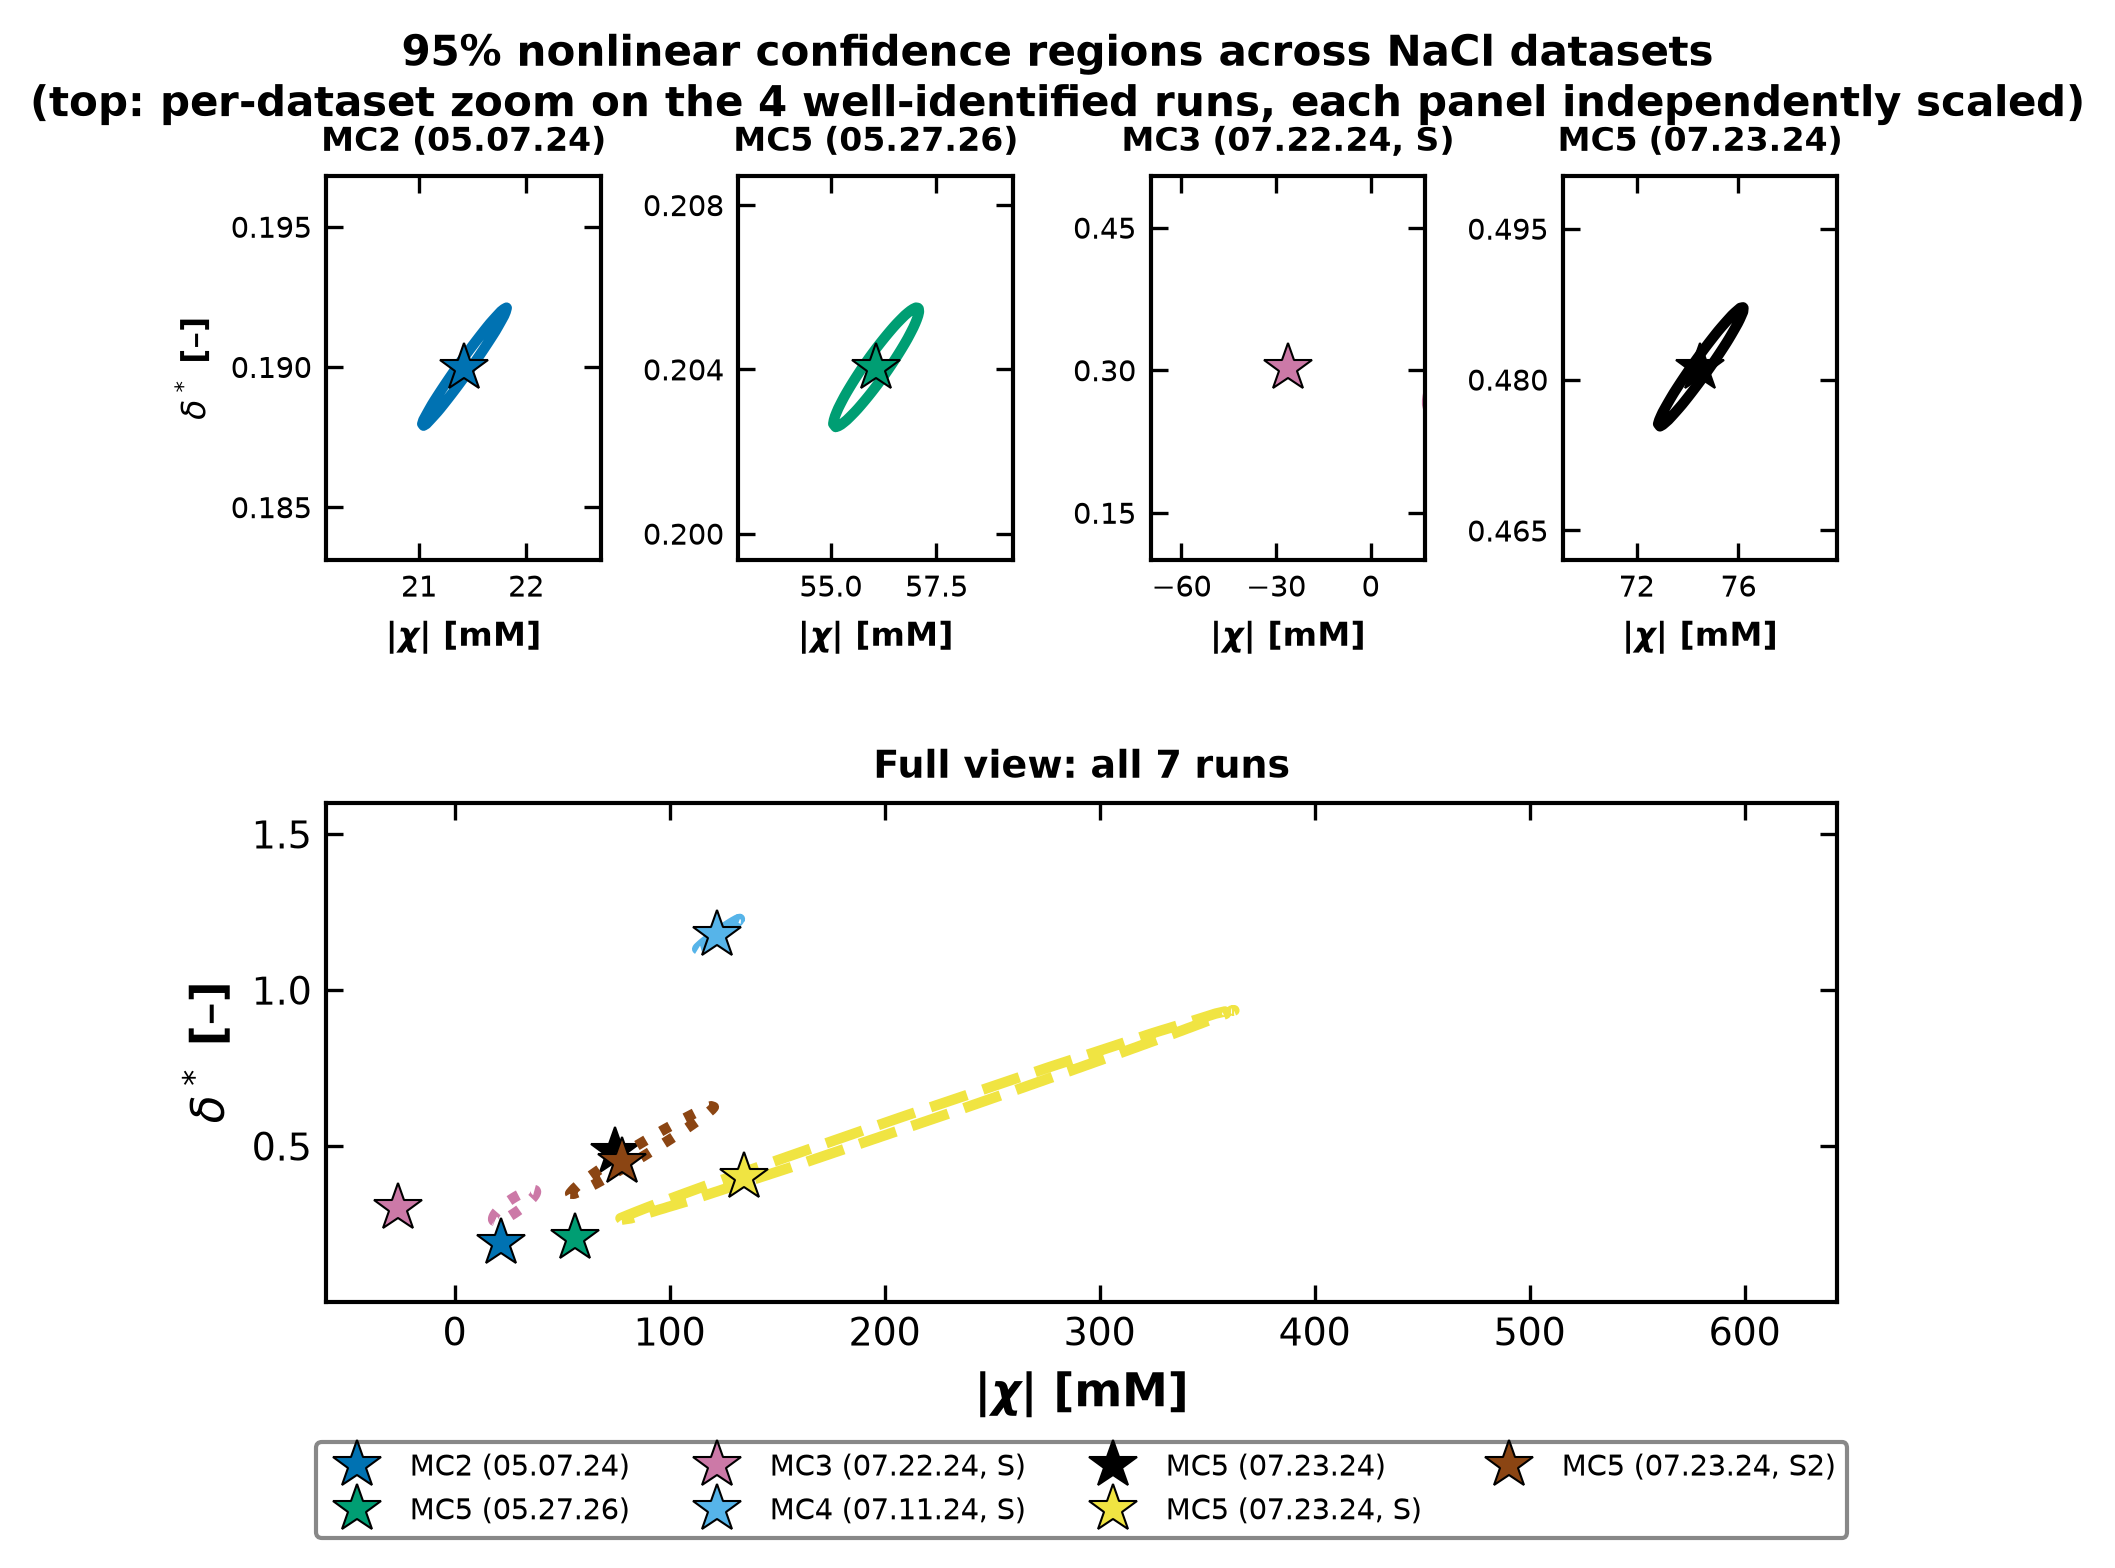
\includegraphics[width=\linewidth]{figures/nacl_all_confidence_regions.png}
\caption{95\% nonlinear (F-test) confidence regions across the seven
non-ill-conditioned \textbf{primary} NaCl datasets (uniformly our-CP; the
the MC5-main comparison row (Estrada's CP) is excluded, Table~\ref{tab:naclall}).
\textbf{Top row}: a per-dataset zoom on the
four \emph{well-identified} runs (95\% CI width $<15\%$ on $|\chi|$) -- each
panel independently scaled to its own optimum $\pm\,8$ SE, so the region
actually renders as a visible ellipse rather than collapsing to a dot.
\textbf{Bottom}: the full view across all seven runs, for context, where the
poorly-identified runs' wide axis range \emph{does} make the tight regions look
like points -- this is a visualization effect, not a numerical one (verified:
the top-row zoom uses the identical \S\ref{sec:stats} F-test region computation
on the identical fits). \emph{Caution:} a tight region reflects internal
\emph{precision}, not accuracy --- MC5 (07.23.24) and MC3 (07.22.24, S) appear
among the well-identified runs yet are \emph{reconstructed}/CP-shifted runs
whose estimates ($|\chi|\approx\SI{75}{mM}$, $\SI{26}{mM}$) are biased away from
the primary MC5 ($\approx\SI{56}{mM}$); only MC2 and MC5(2) (both our-CP,
originally-processed) are both precise \emph{and}
trustworthy. Every dataset has a fixed, distinct color, reused across
Figs.~\ref{fig:naclestimates}--\ref{fig:naclfits}.}
\label{fig:naclall}
\end{figure}

\begin{figure}[H]
\centering
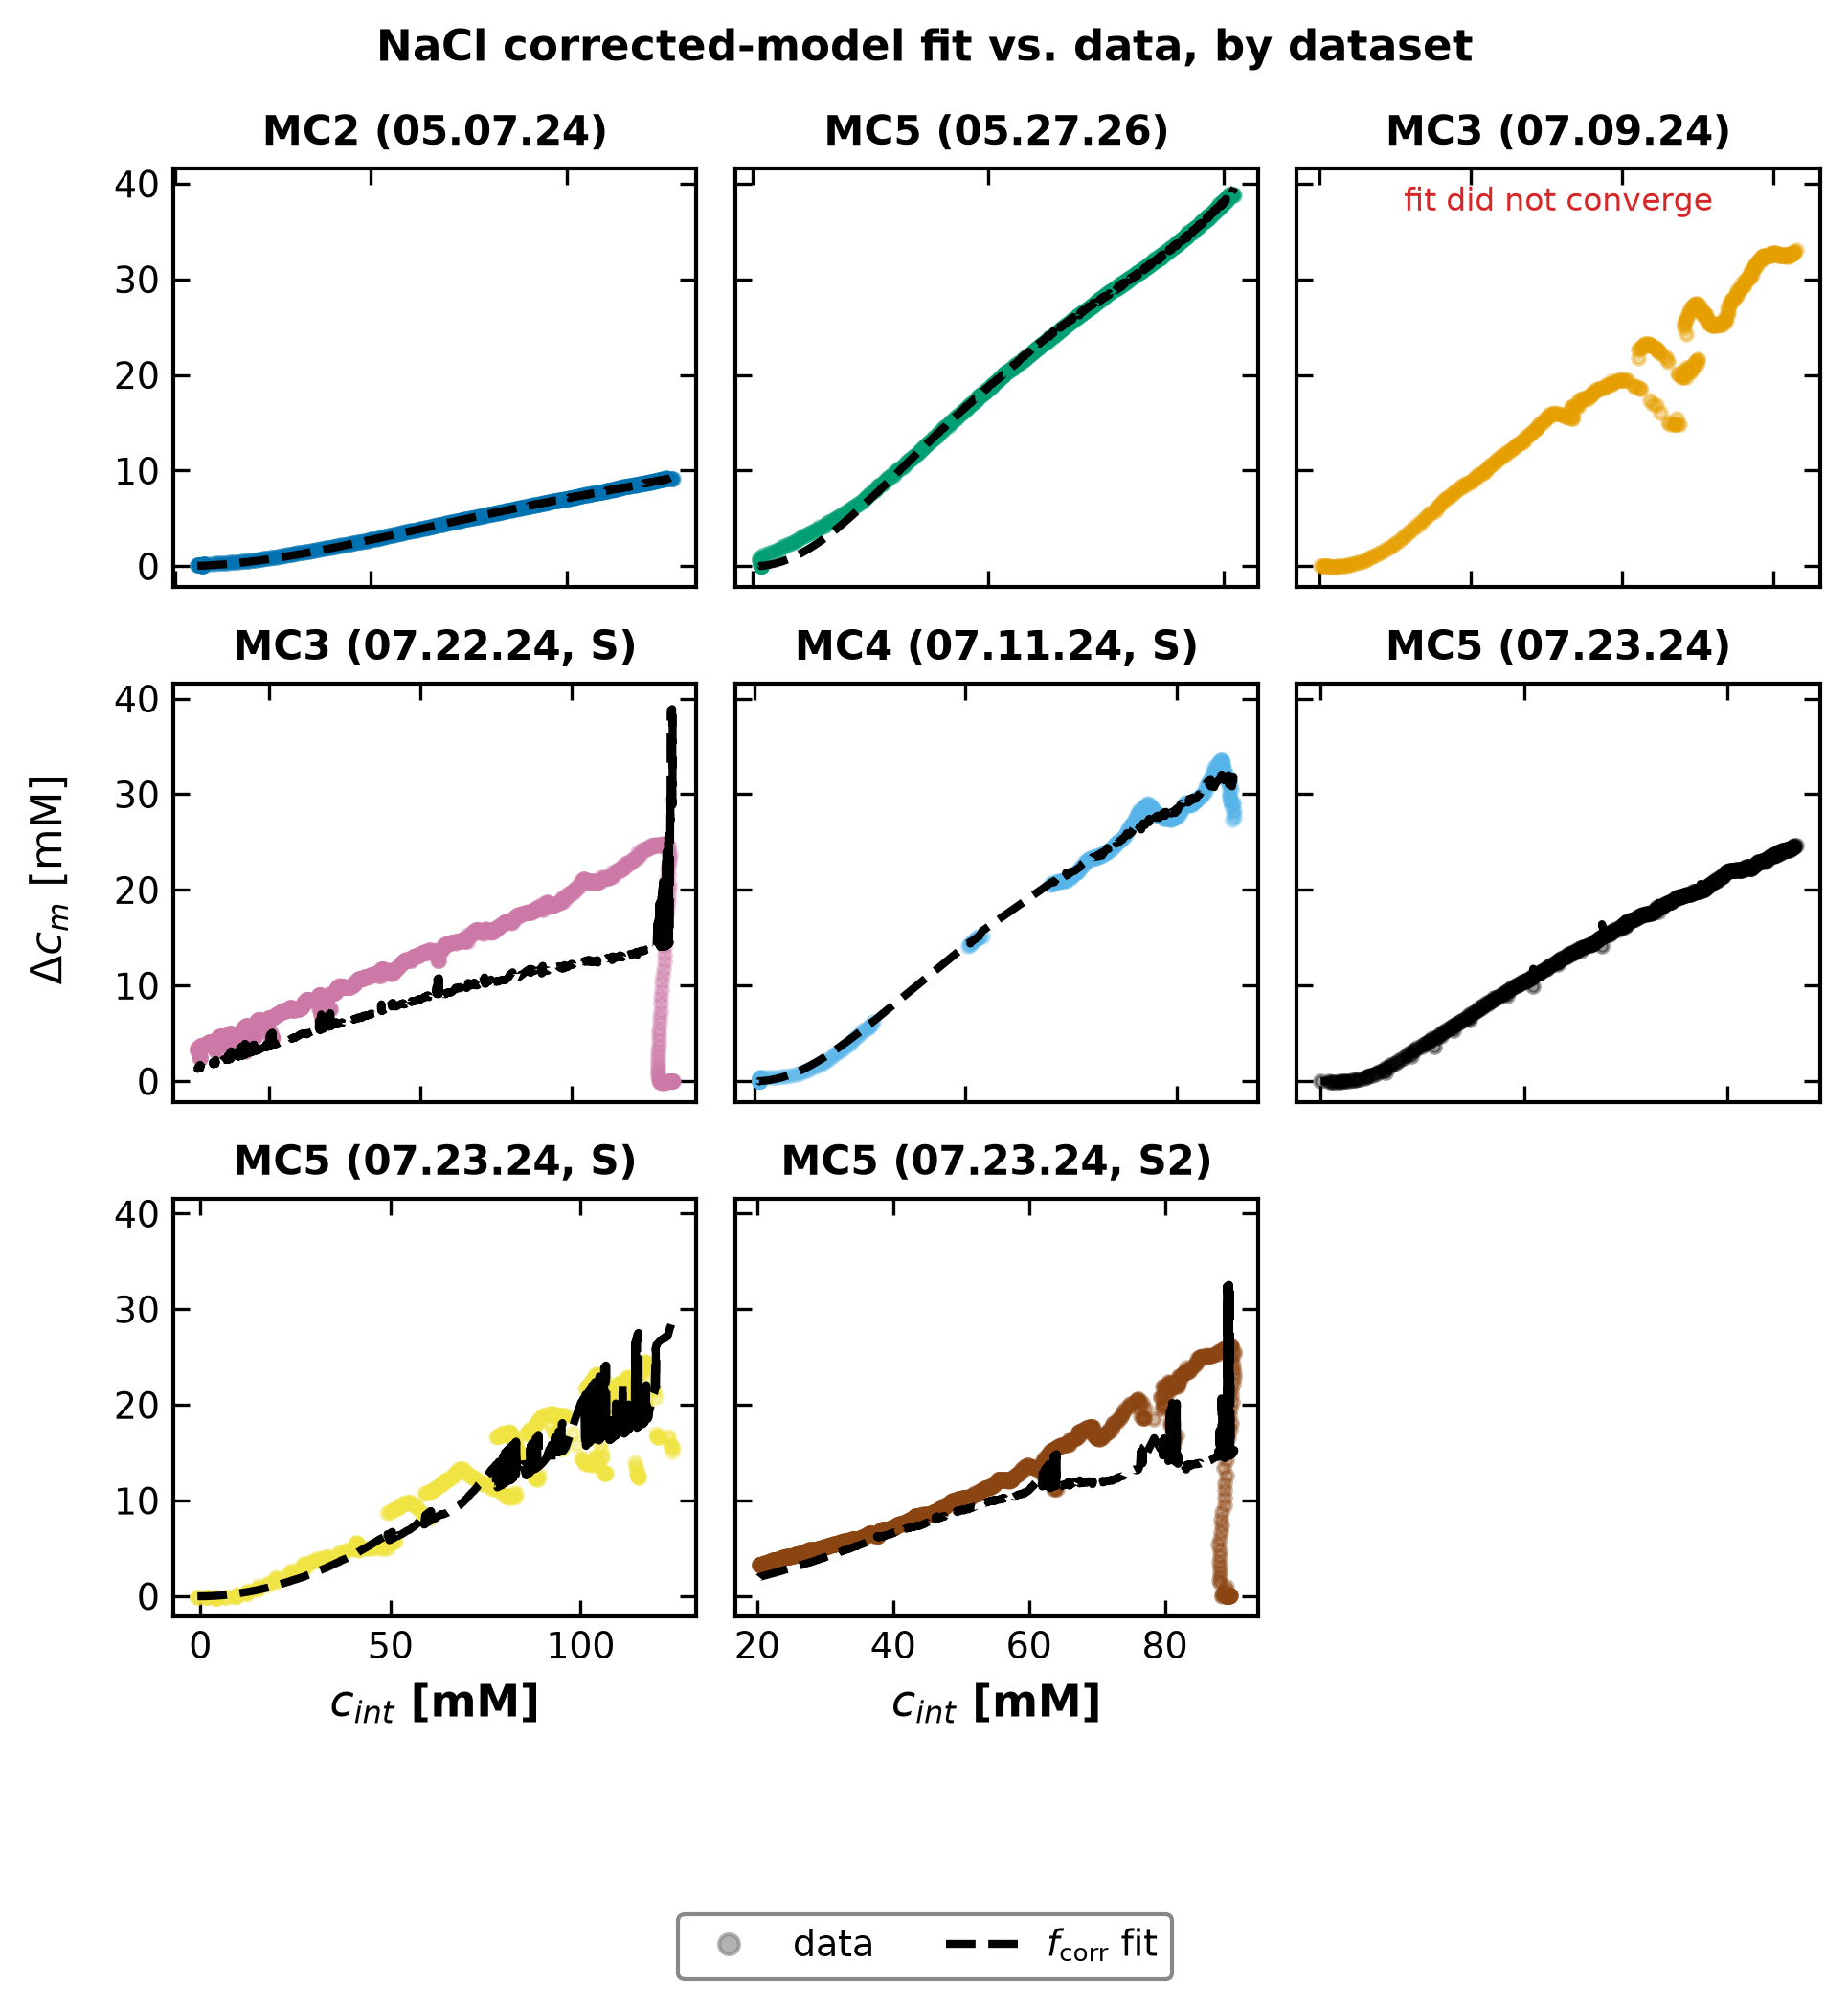
\includegraphics[width=\linewidth]{figures/nacl_all_fits.png}
\caption{Per-dataset fits of the corrected Donnan model to $\Delta c_{\mathrm m}$
for the eight \textbf{primary} (uniformly our-CP) NaCl runs (grid; the
MC5-main comparison row, Estrada's CP, is excluded, Table~\ref{tab:naclall}).
The
two originally-processed runs (MC2, MC5(2)) fit the $1{:}1$ model cleanly; the
six reconstructed raw-only runs are visibly noisier.}
\label{fig:naclfits}
\end{figure}

\subsection{Recommendations and discussion}\label{sec:naclDisc}
\begin{itemize}[itemsep=2pt]
  \item \textbf{MATLAB fix:} restore the $\tfrac12$ in \eqref{eq:matlabmodel} and
        use Levenberg--Marquardt; the current estimates are otherwise a faithful
        (if reparameterized) optimum.
  \item \textbf{Uncertainty:} NaCl is well-identified, but the i.i.d.\ regions
        \emph{were} optimistic as flagged here --- \textbf{this is now
        quantified}: \S\ref{sec:naclAR1} shows the true (AR(1)-corrected)
        regions are $\sim$2.5--2.7$\times$ wider (CP-corrected), and
        \S\ref{sec:altform}
        shows the point estimate itself is sensitive to whether the
        regression is posed on transformed or raw measurements
        ($+140\%$ shift, CP-corrected). Both remain open decisions
        (\S\ref{sec:questions}, items~13--14), not resolved ones.
  \item \textbf{Physical check:} corrected, our-CP primary
        $|\chi|\approx\SI{57}{mM}$
        (MC5(2)$+$our-CP; the MC5-main comparison value, Estrada's own CP, is
        $\approx\SI{50}{mM}$) is the
        value to compare against zeta-potential / literature estimates.
  \item \textbf{Reproducibility (\S\ref{sec:naclAll}):} \textbf{our-CP vs.\
        Estrada's-CP is a real, if minor, implementation discrepancy}: MC5(2)'s
        our-CP $|\chi|=56.07$\,mM is
        $13\%$ above MC5-main's (Estrada's-CP) $49.56$\,mM value (a third
        CP-related sensitivity axis, \S\ref{sec:naclAll}) --- not a
        correctness issue, since both already carry \emph{some} CP
        correction. MC2 (now correctly CP-corrected) vs.\ MC5(2) still
        diverge regardless of CP --- most plausibly a concentration-range
        identifiability effect; prefer wide-range experiments for parameter
        estimation.
  \item \textbf{Current roadmap} (updated --- several items of the
        original list are now \textbf{done}, see \S\ref{sec:synthesis} for the
        cross-salt view): (i) tighten the raw-only NaCl reconstruction
        pipeline (Am/$\rho$, $\Jw$-smoothing,
        \S\ref{sec:questions} items~7--10, 12; CP-vs-non-CP, item~11, is now
        \textbf{resolved} --- CP is the standing convention throughout,
        including the AR(1) and raw-measurement re-runs,
        \S\ref{sec:naclAR1}/\S\ref{sec:altform}); (ii)
        a first-cut concentration-dependent $\chi(c)$ spline has now been
        tried on \ce{CaCl2}'s wide-range data (\S\ref{sec:chispline}) --- the
        constant-charge model is clearly inadequate, but the fitted shape is
        not yet safely interpretable (a follow-up null check found the
        confound is not resolved by a simple AR(1) correction either);
        \textbf{extending the AR(1) correction itself to \ce{CaCl2}/\ce{LaCl3}
        remains pending}; (iii) the multicomponent extension remains deferred
        pending group feedback on the open decisions in
        \S\ref{sec:questions}.
\end{itemize}

% ############################################################
\section{Analysis of \ce{CaCl2} data}\label{sec:cacl2}
% ############################################################
The $2{:}1$ co-ion cubic \eqref{eq:21co} replaces the NaCl quadratic; rather
than its (known but unwieldy) Cardano closed form, we solve it directly (a
fully vectorized closed-form root, \S\ref{sec:cacl2impl}) and fit it to every
available processed \ce{CaCl2} dataset, following the same workflow as
\S\ref{sec:naclAll}. Uncertainty analysis proceeds as in \S\ref{sec:naclUQ}
(profile-likelihood CIs, multi-start).

\paragraph{Working hypothesis: concentration-dependent charge from \ce{Ca^{2+}}
adsorption.} We \emph{expected the \ce{CaCl2} fits to be poorer than NaCl}. The
leading hypothesis is that \ce{Ca^{2+}} adsorbs onto the membrane surface and
alters its effective fixed charge $\chi$, and that this adsorption is
\textbf{concentration dependent}. The present model treats $\chi$ as a single
constant per dataset and does not represent adsorption, so we anticipated (i) a
worse overall fit and (ii) \emph{systematic residual structure versus
concentration} (equivalently, an apparent $\chi$ that drifts with $\cint$). Both
are borne out below, with a more specific finding than anticipated: the global
fit does not merely land on ``some smaller $\chi$ than NaCl'' -- it drives
$|\chi|$ to (numerically) zero for all three datasets, deferring all of the
partitioning behavior to the lumped constant $K$ (see \eqref{eq:cacl2model}).

\subsection{Model, datasets, and implementation}\label{sec:cacl2impl}
\paragraph{Co-ion and stoichiometry.} Co-ion $=\ce{Cl-}$; its solution
concentration is set by stoichiometry, $\cs{\co}=2\,c_{\ce{CaCl2}}$ ($2\,\ce{Cl-}$
per \ce{CaCl2}), applied at both the feed face ($\cint$) and permeate face
($\cp$).

\paragraph{Governing equation.} We fit the $2{:}1$ cubic \eqref{eq:21co} with a
single \textbf{lumped partition constant} $K\ge0$ absorbing $\dstar\,
\delta^{\circ}_{\co}$ and constant stoichiometric factors:
\begin{equation}
  \cm{\co}^3 + |\chi|\,\cm{\co}^2 - K\,\cs{\co}^3 = 0,
  \qquad \text{prediction} = \cm{\co}(\cint) - \cm{\co}(\cp),
  \label{eq:cacl2model}
\end{equation}
solved for the unique positive real root (Descartes' rule of signs guarantees
exactly one, for any real $|\chi|$). The transformed response mirrors the
corrected NaCl form, but on the \ce{Cl-} flux (twice the \ce{CaCl2} molar flux,
by stoichiometry):
\begin{equation}
  \Delta c_{\mathrm m} = \frac{J_{s,\ce{Cl}}\,\ell}{D_{\ce{CaCl2},m}},
  \qquad J_{s,\ce{Cl}} = 2\,\cp\,\Jw,
  \qquad D_{\ce{CaCl2},m}=\frac{3\,D_{\ce{Ca},m} D_{\ce{Cl},m}}{2D_{\ce{Ca},m}+D_{\ce{Cl},m}},
  \label{eq:cacl2response}
\end{equation}
with membrane-phase diffusivities $D_{\ce{Ca},m}=\SI{0.79e-12}{m^2/s}$,
$D_{\ce{Cl},m}=\SI{2.03e-12}{m^2/s}$ (same $\sim\!1000\times$ solution-to-membrane
scaling Bill used for NaCl) and $\ell=\SI{80}{nm}$ as before. We fit $(|\chi|,K)$
to $\Delta c_{\mathrm m}$ by \texttt{scipy.optimize.least\_squares}, with
$|\chi|,K\ge0$ \textbf{bounded} (\texttt{method="trf"}) rather than
unconstrained \texttt{lm}: unlike the NaCl model, where $\beta_1$ only ever
appears squared inside a square root (so its sign cannot matter), $|\chi|$
enters \eqref{eq:cacl2model} unsquared and asymmetrically, so an unconstrained
fit can drift to a spurious negative ``$\chi$'' with a negligibly lower SSE and
no physical meaning (confirmed empirically: $-0.06\%$ SSE change for a sign
flip on MC5 05.27.26). These are Opus's working assumptions (per the task
prompt to Sonnet), chosen to mirror the NaCl treatment closely enough to be
directly comparable; a lumped-constant prefactor mismatch in $K$ would bias
absolute $|\chi|$/$K$ values but \emph{not} the residual-shape/drift
diagnostics that are the point of this section. \note{Confirm the $2{:}1$
non-ideal factor split ($\dstar\,\delta^{\circ}_{\co}$ vs.\ $K$ alone) with the
group -- discussion point in \S\ref{sec:donnan}.}

\paragraph{Root-solve implementation.} Rather than a per-point
\texttt{numpy.roots} call (correct but far too slow at these array sizes,
$n$ up to $\sim\!1900$, called repeatedly inside multi-start and the
sliding-window diagnostic below), \texttt{analysis/cacl2/regress\_cacl2.py}
solves \eqref{eq:cacl2model} with a fully vectorized closed-form root in two
regimes, selected by how small the true root is relative to $|\chi|$: an
asymptotic-balance-plus-Newton-polish branch (avoiding the catastrophic
cancellation a general Cardano solve suffers there) and a general complex
Cardano branch otherwise. Verified against \texttt{numpy.roots} on a
5000-point random parameter scan to $<10^{-9}$ relative error with zero
non-finite outputs (\texttt{analysis/cacl2/README.md}).

\paragraph{Datasets.} All three processed \ce{CaCl2} sheets, read from
\texttt{data/BoE Analysis.xlsx} (the 27-sheet superset; \emph{not}
\texttt{data/Rejection\_Analysis.xlsx}, which is missing the 06.27.26 run),
same 15-column schema as NaCl (columns B/H/J):

\begin{table}[H]
\centering\small
\begin{tabular}{llrl}
\toprule
Memb. & Sheet & Valid rows & $\cint$ range \\
\midrule
MC3 & \texttt{NF270\_MC3 07.11.24\_SCaCl2} & 609 & $1.0$--$47$\,mM \\
MC5 & \texttt{NF270\_MC5 05.27.26\_CaCl2}  & 1645 & $1.6$--$108$\,mM \\
MC5 & \texttt{NF270\_MC5 06.27.26\_CaCl2}  & 1885 & $1.3$--$103$\,mM \\
\bottomrule
\end{tabular}
\caption{The three processed \ce{CaCl2} datasets analyzed in this section. The
MC5 05.27.26 vs.\ 06.27.26 pair is a near-repeat (reproducibility check, see
below). \textbf{Not yet processed} (raw-only, out of scope here): MC2
05.07.24, MC3 07.11.24\_\ce{CaCl2}, MC3 07.12.24\_S2\ce{CaCl2}, and the
mislabeled tab \texttt{NF270\_MC5 05.26.26\_NaCl} (its own note identifies it
as \ce{CaCl2}, not NaCl -- also excluded from the NaCl accounting,
Table~\ref{tab:nacldata}).}
\label{tab:cacl2data}
\end{table}

\subsection{Results: all three datasets}\label{sec:cacl2results}
\textbf{All three processed \ce{CaCl2} runs were regressed} with the bounded
$(|\chi|,K)$ model, full valid range, \textbf{CP applied on top of the
processed-sheet
bulk} $\cint$ (all three sheets are the non-CP convention, \S\ref{sec:preproc}
raw-reprocessing validation; $k_{\ce{CaCl2}}=\SI{2.25e-5}{m/s}$). Table~\ref{tab:cacl2all}
reports all three together; Figure~\ref{fig:cacl2fits} shows the per-dataset
fits and Figure~\ref{fig:cacl2estimates} the point estimates with 95\%
profile-likelihood CIs. \emph{Full fit/residual/drift detail for every
individual run is in the appendix, \S\ref{sec:cacl2appendix} (not yet refreshed
to these CP-corrected numbers).}

\begin{table}[H]
\centering\small\setlength{\tabcolsep}{4pt}
\begin{tabular}{lrccccc}
\toprule
Dataset & $n$ & $|\chi|$ [\si{mM}] (95\% CI) & $K$ (95\% CI) & SSE & pseudo-$R^2$ & MS \% \\
\midrule
MC3 (07.11.24, S) & 609  & $0.0000\ (0.000,\,34.4)$  & $0.01116\ (0.01100,\,0.01130)$ & $147.1$  & $0.979$ & $100\%$\\
MC5 (05.27.26)     & 1645 & $2.9466\ (2.288,\,3.596)$ & $0.00057\ (0.00056,\,0.00058)$ & $418.3$  & $0.959$ & $99\%$\\
MC5 (06.27.26)     & 1885 & $0.0494\ (0.000,\,0.617)$ & $0.00023\ (0.00022,\,0.00023)$ & $666.5$  & $0.892$ & $96\%$\\
\bottomrule
\end{tabular}
\caption{\ce{CaCl2} regression, all three datasets, \textbf{CP-corrected
(primary)}, bounded $2{:}1$ cubic model, full valid range; 95\% CIs are
profile-likelihood; MS = multi-start \% reaching the global optimum, 100 random
starts. \textbf{CP sharpens, but does not overturn, the headline finding:}
$|\chi|$ is still pinned at (or extremely close to) zero for two of the three
datasets; MC5 (05.27.26) --- the widest-range dataset --- now resolves to a
small but statistically \emph{nonzero} $|\chi|\approx\SI{2.9}{mM}$ (CI excludes
zero), still $\approx19\times$ smaller than \ce{NaCl}'s $\approx\SI{57}{mM}$. Fit
quality improves under CP across the board (pseudo-$R^2$: $0.84$--$0.95\to
0.89$--$0.96$). MC3's much wider CI
reflects its narrower concentration range ($\lesssim\SI{47}{mM}$ vs.\ MC5's
$\gtrsim\SI{100}{mM}$), the same range-identifiability effect noted for NaCl's
MC2 vs.\ MC5 (\S\ref{sec:naclAllResults}).}
\label{tab:cacl2all}
\end{table}

\begin{figure}[H]
\centering
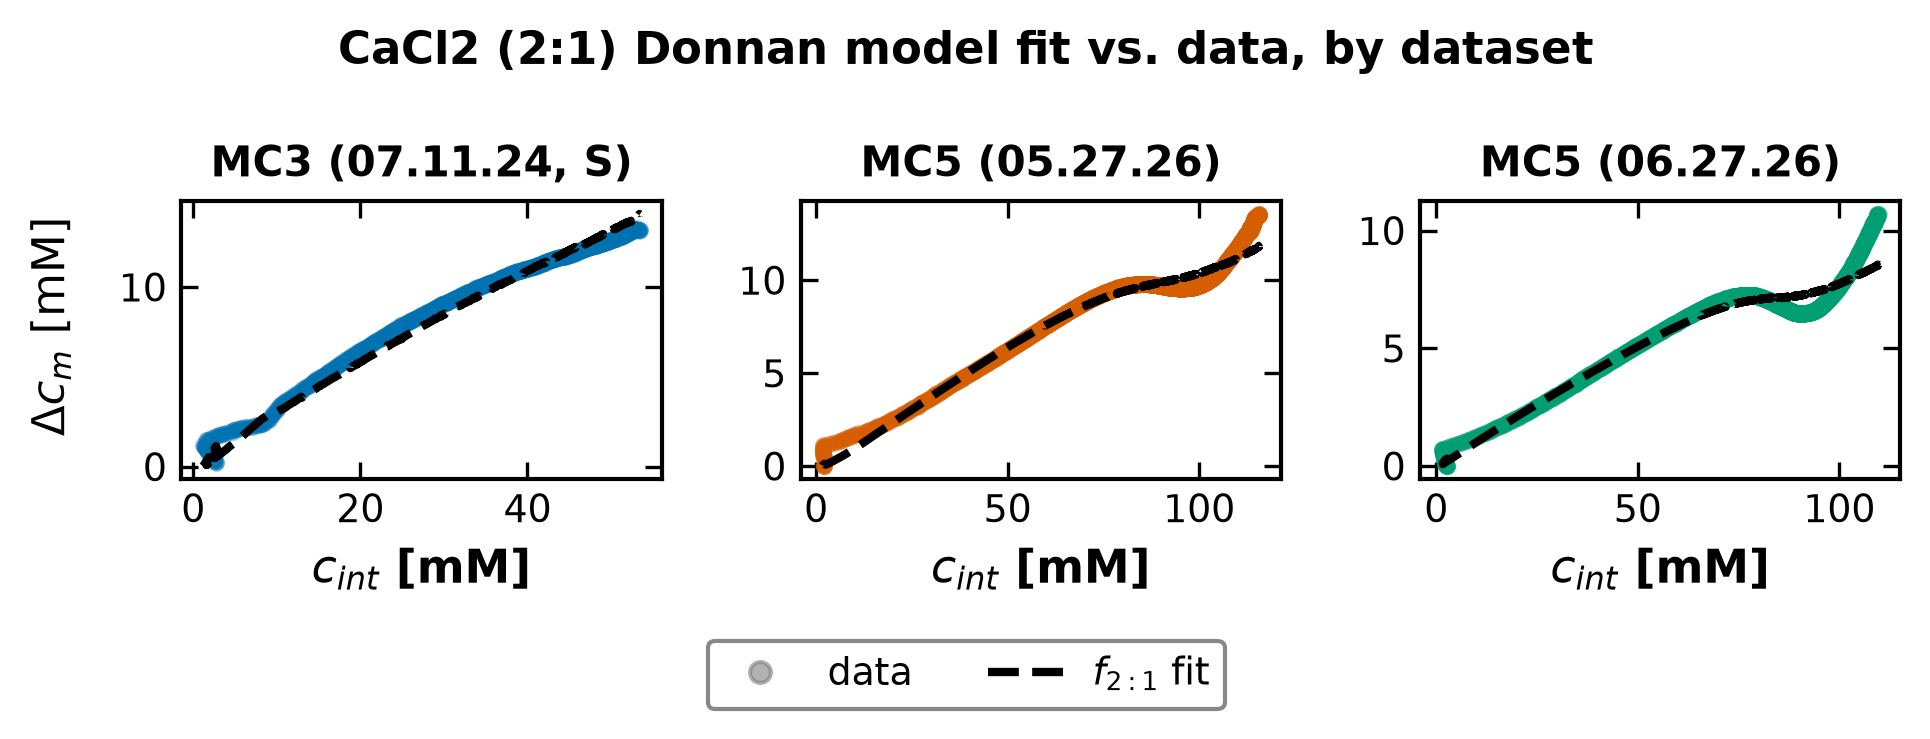
\includegraphics[width=\linewidth]{figures/cacl2_fits.png}
\caption{\ce{CaCl2} corrected-model ($2{:}1$ cubic) fit vs.\ data, by dataset.
The model tracks the overall trend, but see Figure~\ref{fig:cacl2resid} for the
systematic residual structure the point estimate above does not reveal.}
\label{fig:cacl2fits}
\end{figure}

\begin{figure}[H]
\centering
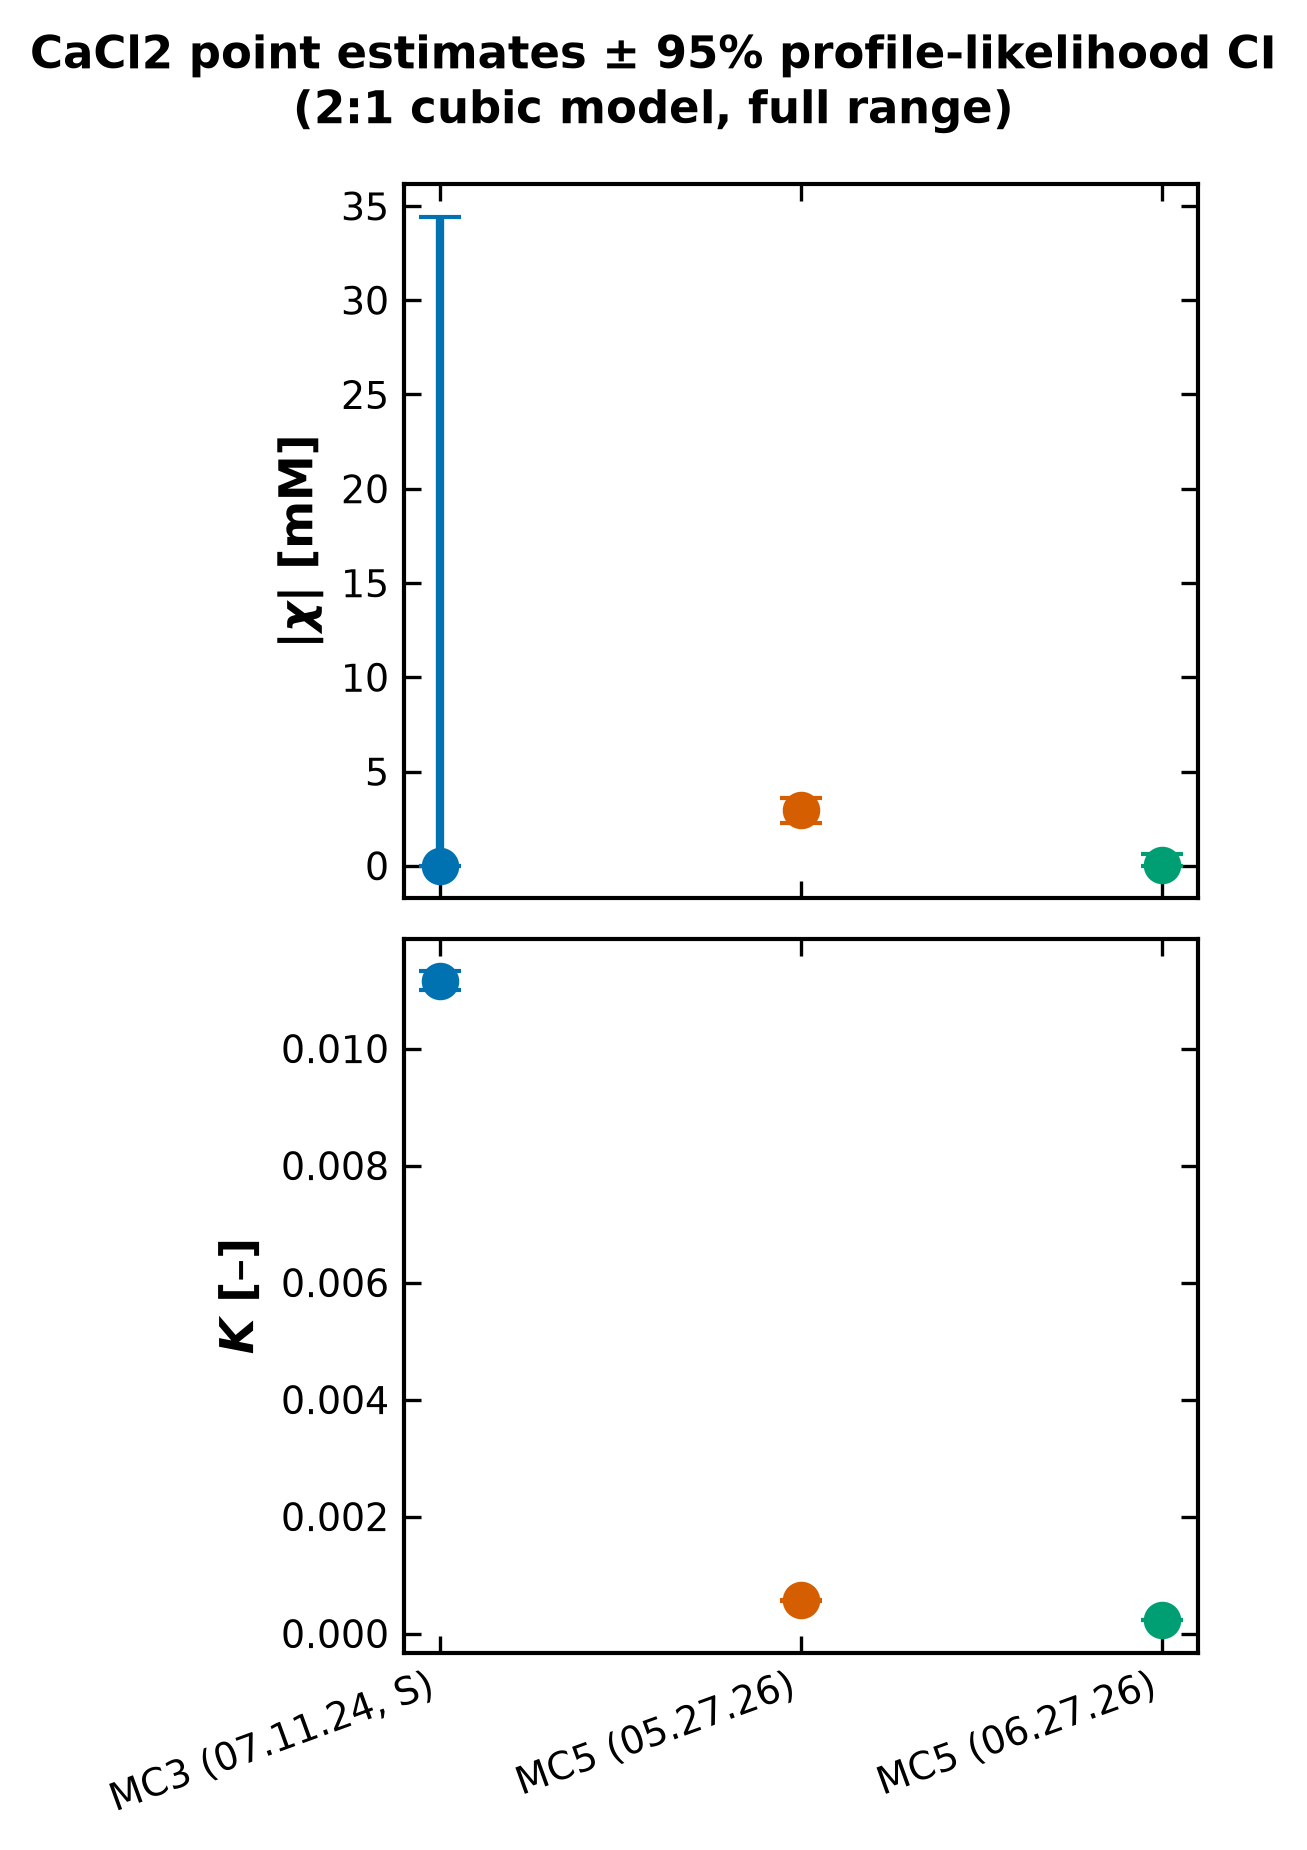
\includegraphics[width=0.6\linewidth]{figures/cacl2_estimates.png}
\caption{\ce{CaCl2} point estimates $\pm$ 95\% profile-likelihood CI, all
three datasets, CP-corrected. The two MC5 runs no longer fully agree under CP
(05.27.26's CI excludes zero, 06.27.26's does not); MC3's much
wider $|\chi|$ CI reflects weaker identifiability at its narrower
concentration range.}
\label{fig:cacl2estimates}
\end{figure}

\subsection{Adsorption-hypothesis diagnostics}\label{sec:cacl2diag}
\paragraph{Residuals vs.\ concentration (Figure~\ref{fig:cacl2resid}).} All
three datasets show a clear, smooth, \emph{non-random} wave pattern (CP-corrected,
as on non-CP). A sign-runs test (fewer sign changes
than random residuals would produce) is strongly significant for all three
($z=-23.1$, $-39.2$, $-42.3$ for MC3, MC5 05.27.26, MC5 06.27.26 respectively --
$z$ this far from 0 simply confirms the visually obvious structure is not
noise). This matches the anticipated signature: the single-$|\chi|$ model
cannot capture whatever concentration-dependent physics is really at play.

\begin{figure}[H]
\centering
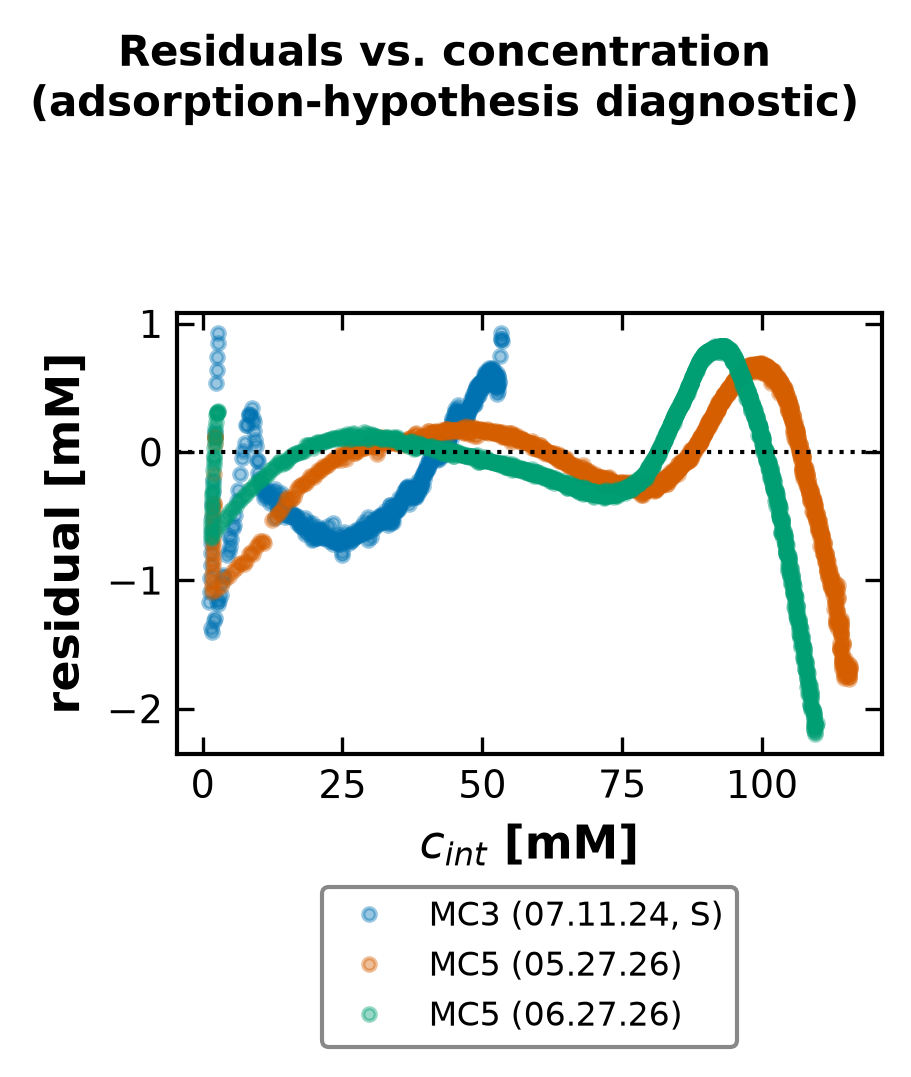
\includegraphics[width=0.49\linewidth]{figures/cacl2_residuals_vs_conc.png}\hfill
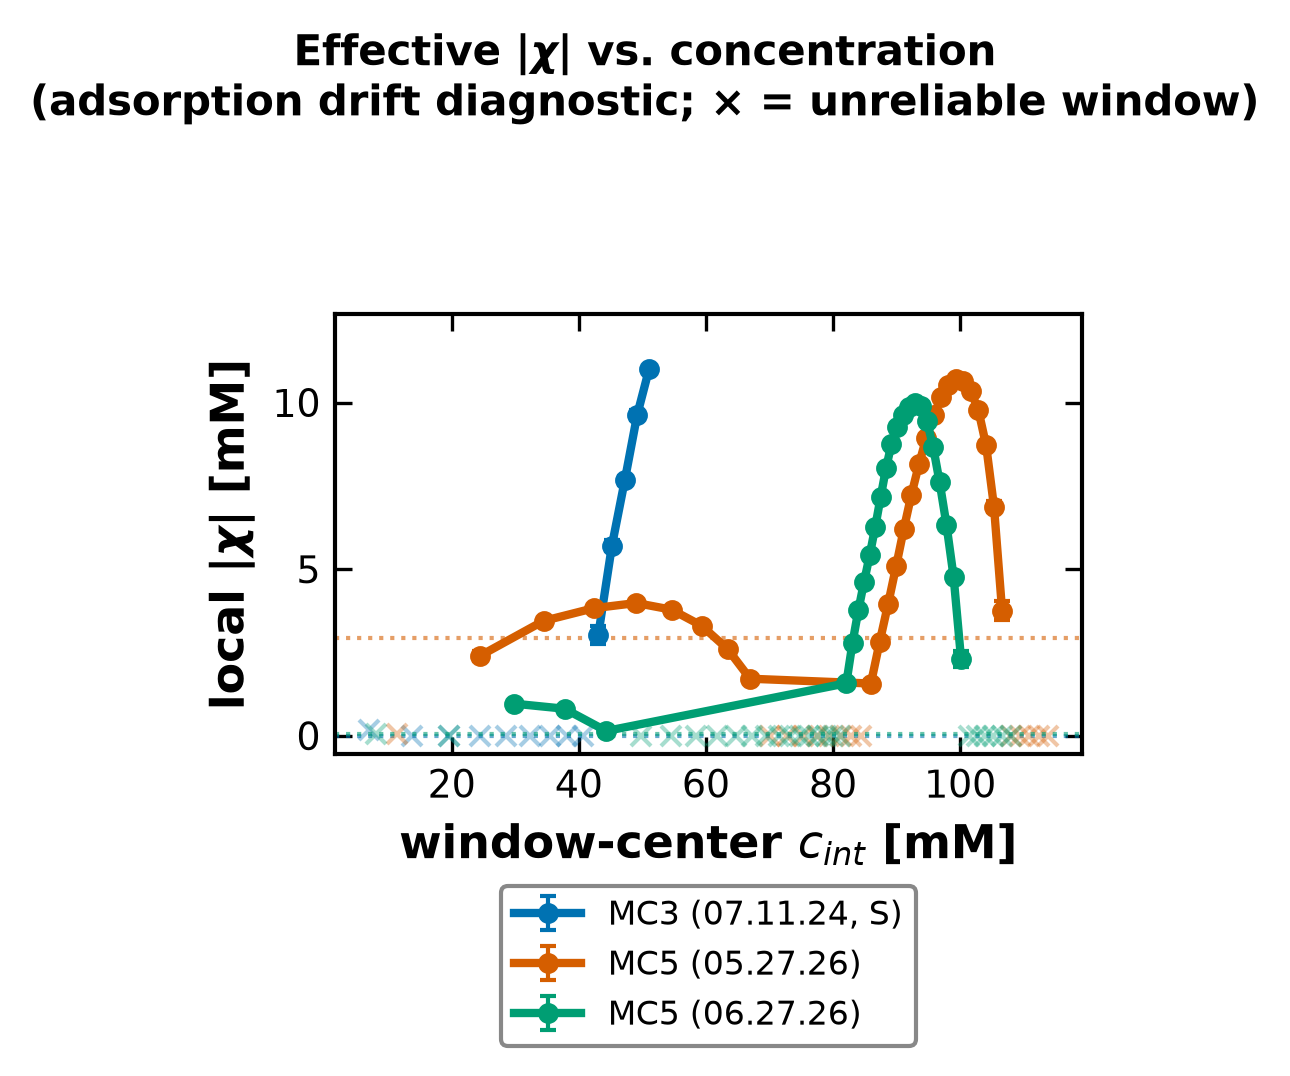
\includegraphics[width=0.49\linewidth]{figures/cacl2_effective_chi_vs_conc.png}
\caption{\textbf{Left:} residuals vs.\ $\cint$ -- the key adsorption-hypothesis
diagnostic; all three datasets show the same smooth non-random wave shape.
\textbf{Right:} sliding-window (80 points/window) local $|\chi|$ refits ($K$
fixed at the global estimate); unreliable windows (large SE or pinned at the
window search-box bound, mostly at very low $\cint$) shown as faint $\times$
and excluded from the trend read below.}
\label{fig:cacl2resid}
\end{figure}

\paragraph{Effective $|\chi|$ vs.\ concentration (Figure~\ref{fig:cacl2resid},
right).} \emph{Method} (used here, in \S\ref{sec:lacl3diag}, and as the
model-free cross-check in \S\ref{sec:chispline}): sort the run by $\cint$ and
slide a fixed-size window along it ($80$ consecutive points, stride $40$); within
each window $W_j$ refit a \emph{single local} charge, holding the partition
constant at its global value $\hat K$,
\begin{equation}
  \hat\chi_j=\arg\min_{\chi\in[\varepsilon,\,\chi_{\max}]}
  \sum_{i\in W_j}\Big[\Delta c_{\mathrm m}^{(i)}
   -\big(\cm{\co}(\cint^{(i)};\chi,\hat K)-\cm{\co}(\cp^{(i)};\chi,\hat K)\big)\Big]^2,
  \label{eq:effchi}
\end{equation}
and plot $\hat\chi_j$ against the window-mean concentration
$\bar c_j=\tfrac{1}{|W_j|}\sum_{i\in W_j}\cint^{(i)}$. A window is flagged
\emph{unreliable} (faint $\times$, excluded from the trend) when $\hat\chi_j$
pins at the search bound $\chi_{\max}$ or its local Wald standard error is large
relative to $\hat\chi_j$ --- i.e.\ its narrow $\cint$ sub-range does not identify
a local charge. Holding $\hat K$ fixed makes each $\hat\chi_j$ a one-parameter
read of how much fixed charge that concentration slice \emph{alone} implies; it
is a \emph{diagnostic} of whether a single constant charge suffices, not a fitted
$\chi(c)$ model (that is \S\ref{sec:chispline}). Both MC5 runs still show a
\textbf{non-monotonic (inverted-U) drift}
under CP: local $|\chi|$ rises from near 0 at low $\cint$ to a peak of
$\sim\!10$--$11$\,mM around $\cint\approx90$--$100$\,mM, then falls back down at
the highest concentrations. MC3's few reliable windows (5 of 14; the rest are
too weakly identified over its narrow range to trust and are excluded from the
trend) rise from $\sim\!3$ to $\sim\!11$\,mM over its range -- consistent with
sitting on the same \emph{rising} leg MC5 shows over a wider range. \note{This
is drift, but not a simple monotonic one: a naive ``adsorption increases with
concentration, monotonically suppressing $|\chi|$'' story predicts a monotonic
\emph{decrease}; what is observed is a rise-then-fall. Two non-exclusive
readings: (i) Ca$^{2+}$ adsorption may already be saturated/screening the
charge even at low $\cint$, with the mid-range rise-then-fall reflecting an
unaccounted effect such as concentration polarization (not corrected for
\ce{CaCl2} here, \S\ref{sec:cp}); or (ii) the windowed local-refit
diagnostic's shape may be partly an artifact of how each window's $\cint$
sub-range interacts with the $K$ held fixed at the global estimate, rather
than a direct read of the physics. Either way, $|\chi|$ is clearly not flat
with concentration for any of the three datasets -- worth resolving with the
group before committing to a specific $|\chi|(c)$ functional form.}

\paragraph{Reproducibility: MC5 05.27.26 vs.\ 06.27.26.} \textbf{CP separates
these two runs that previously agreed}: under CP, 05.27.26 resolves to a small
but nonzero $|\chi|=2.95$\,mM (CI excludes 0) while 06.27.26 stays pinned near
zero ($0.049$\,mM, CI includes 0) -- their CIs no longer overlap. 06.27.26 still
has a visibly worse pseudo-$R^2$ ($0.892$ vs.\
$0.959$) -- worth a follow-up
look at whether 06.27.26 has more noise or a genuinely different
high-concentration behavior (e.g.\ a different membrane fouling state on that
date), and now also whether the CP shift itself is partly responsible for the
split.

\paragraph{Verdict.} \textbf{The adsorption hypothesis is supported, with a
specific and unexpected refinement -- and CP sharpens rather than overturns
it.} The fit is materially different from NaCl's (chi pinned at/near $0$ for
two of three datasets vs.\ NaCl's clean $18$--$57$\,mM), residuals
show strong, consistent, non-random structure vs.\ concentration in all three
datasets, and the local effective $|\chi|$ demonstrably drifts with
concentration rather than staying flat -- all as anticipated. That the
\emph{global} fit drives $|\chi|$ to (near) zero for two of three datasets,
rather than landing on ``some smaller nonzero value than NaCl,'' is a sharper
piece of evidence than expected; MC5 (05.27.26)'s CP-corrected
$|\chi|\approx\SI{2.9}{mM}$ is the exception (small but statistically
significant, still $\approx19\times$ below NaCl), consistent with the local drift
diagnostic already showing nonzero effective $|\chi|$ over parts of that same
dataset's range -- a single global constant necessarily averages that
concentration-dependence away. The non-monotonic shape of that drift is the
open question for follow-up --
most likely resolved by either a concentration-dependent $|\chi|(c)$ model
extension or ruling out concentration-polarization/window-diagnostic artifacts
first (see the note above) -- concentration polarization is no longer
uncorrected-for at the global-fit level (this section), but the sliding-window
diagnostic itself does not re-derive CP locally per window.

% ############################################################
\section{Analysis of \ce{LaCl3} data}\label{sec:lacl3}
% ############################################################
The $3{:}1$ co-ion quartic \eqref{eq:31co} has \textbf{no compact closed
form} (unlike NaCl's quadratic or \ce{CaCl2}'s cubic). Rather than coding an
explicit (numerical) quartic solution as the only route, this section fits
it \textbf{two independent ways and cross-checks} them, mirroring
\S\ref{sec:naclUQ}'s scipy-vs-ParmEst validation: (A) a bracketed root-find
per point, driving a \texttt{scipy.optimize.least\_squares} fit; (B) the
membrane co-ion concentration introduced as a Pyomo decision \emph{variable},
\textbf{constrained} by the quartic (positivity-bounded to select the
physical root), estimated via ParmEst/Ipopt. Method B needs no closed-form
root or explicit residual function at all --- it is the formulation that
\textbf{generalizes directly to the eventual multicomponent extension}, where no
closed form exists for any salt combination, so validating it here is
directly useful beyond \ce{LaCl3} itself.

\subsection{Model, dataset, and implementation}\label{sec:lacl3impl}
\paragraph{Co-ion, stoichiometry, and governing equation.} Co-ion $=\ce{Cl-}$;
$\cs{\co}=3\,c_{\ce{LaCl3}}$ ($3\,\ce{Cl-}$ per LaCl3), at both $\cint$ and
$\cp$. We fit the $3{:}1$ quartic \eqref{eq:31co} with a lumped constant
$K\ge0$ absorbing $\dstar(\delta^{\circ}_{\co})^2$ and stoichiometric factors:
\begin{equation}
  \cm{\co}^4 + |\chi|\,\cm{\co}^3 - K\,\cs{\co}^4 = 0,
  \qquad \text{prediction} = \cm{\co}(\cint) - \cm{\co}(\cp),
  \label{eq:lacl3model}
\end{equation}
with a unique positive real root (Descartes: sign pattern $+,+,0,0,-$). The
transformed response mirrors CaCl2's form, on the $3\times$ \ce{Cl-} flux:
$\Delta c_{\mathrm m}=J_{s,\ce{Cl}}\ell/D_{\ce{LaCl3},m}$,
$J_{s,\ce{Cl}}=3\cp\Jw$, $D_{\ce{LaCl3},m}=\frac{4D_{\ce{La},m}D_{\ce{Cl},m}}{3D_{\ce{La},m}+D_{\ce{Cl},m}}$,
$D_{\ce{La},m}=\SI{0.626e-12}{m^2/s}$, $D_{\ce{Cl},m}=\SI{2.03e-12}{m^2/s}$,
$\ell=\SI{80}{nm}$. As for \ce{CaCl2}, $(|\chi|,K)$ are fit \textbf{bounded
$\ge0$}: $|\chi|$ enters \eqref{eq:lacl3model} unsquared/asymmetrically, so an
unconstrained fit can drift to a spurious negative value with no physical
meaning. These are Opus's working assumptions (mirroring \S\ref{sec:cacl2impl}),
sufficient for the hypothesis test; a lumped-constant prefactor mismatch would
bias absolute $|\chi|$/$K$ but not the residual-shape/drift diagnostics.
\note{Confirm the $3{:}1$ non-ideal factor $(\delta^{\circ}_{\co})^2$ vs.\ $K$
alone with the group, as for \ce{CaCl2} -- \S\ref{sec:donnan}.}

\paragraph{Method A: bracketed root-find.} A per-point Brent search
(expanding-bracket for the upper endpoint), verified against
\texttt{numpy.roots} on a 3000-point random parameter scan to $<10^{-6}$
relative error, $\sim\!2.5\times$ faster than a per-point \texttt{numpy.roots}
call at this dataset's scale ($n=623$).

\paragraph{Method B: ParmEst nonlinear-constraint quartic.} Each experiment
introduces auxiliary Vars $\cm{\co,f},\cm{\co,p}$ (membrane co-ion
concentration at the feed/permeate face), each bounded positive and
constrained by \eqref{eq:lacl3model} at that face's $\cs{\co}$; the response
constraint is $\Delta c_{\mathrm m}=\cm{\co,f}-\cm{\co,p}$. ParmEst/Ipopt
solves the joint extensive-form NLP over all experiments, tying $(|\chi|,K)$
to shared decision variables --- no explicit residual function or root
formula appears anywhere in this formulation.

\paragraph{Dataset.} One processed \ce{LaCl3} run: \texttt{NF270\_MC2
05.21.24\_LaCl3} in \texttt{data/BoE Analysis.xlsx} (also in
\texttt{Rejection\_Analysis.xlsx}), $n=623$, standard 15-column schema.
\textbf{Narrow concentration range}, $\cint\approx2$--$\SI{28}{mM}$. A
raw-only \texttt{MC4 07.11.24\_SLaCl3} run exists in the raw campaign
workbook but is \textbf{out of scope here} (would need the preprocessing
pipeline of \S\ref{sec:preproc}; noted as future work, as the raw-only NaCl
runs were before \S\ref{sec:naclAll}'s pipeline was built).
\textbf{Anticipated headwinds} (both realized below): (i) the narrow range
gives weak $|\chi|$ identifiability, the same effect flagged for NaCl's MC2
and \ce{CaCl2}'s MC3 (07.11.24, S); (ii) low \ce{La^{3+}} rejection may
ill-condition the fit.

\subsection{Results}\label{sec:lacl3results}
\begin{table}[H]
\centering\small
\begin{tabular}{lrcccc}
\toprule
Dataset & $n$ & $|\chi|$ [\si{mM}] (95\% CI) & $K$ (95\% CI) & SSE & pseudo-$R^2$ \\
\midrule
MC2 (05.21.24) & 623 & $0.0000\ (0.000,\,34.48)$ & $3.281\times10^{-8}\ (3.163,\,3.404)\times10^{-8}$ & $4.633$ & $0.906$ \\
\bottomrule
\end{tabular}
\caption{\ce{LaCl3} regression, \textbf{CP-corrected (primary)}, bounded
$3{:}1$ quartic model, Method A, full valid range ($k_{\ce{LaCl3}}=\SI{2.21e-5}{m/s}$,
CP applied on top of Ouimet's processed-sheet bulk $\cint$ -- this sheet is the non-CP
convention, \S\ref{sec:preproc} raw-reprocessing validation); 95\% CI is
profile-likelihood; 100\% multi-start convergence, 100 starts. \textbf{One
processed \ce{LaCl3} dataset is analyzed here} --
the raw-only MC4 run (\S\ref{sec:lacl3impl}) is future work. \textbf{$|\chi|$
is pinned at its lower bound} ($\ge0$), even more extremely than
\ce{CaCl2}'s near-zero estimates (Table~\ref{tab:cacl2all}), and \textbf{CP
narrows the CI and improves fit quality} (pseudo-$R^2$: $0.803\to0.906$;
non-CP CI was $(0,\SI{94}{mM})$).}
\label{tab:lacl3}
\end{table}
\note{This is a \emph{boundary} solution, not an interior optimum: the CI
$(0,\SI{34}{mM})$ is one-sided against the $|\chi|\ge0$ bound. $|\chi|$ is
therefore essentially \textbf{unidentified} from this dataset, not
``measured to be $0$'' --- the data are simply uninformative about it in
either direction.}

\paragraph{Method A vs.\ Method B agreement.} ParmEst (warm-started at
Method A's converged root, for a fair, strong comparison) gives
$|\chi|=1.196\times10^{-3}$\,mM, $K=3.28128\times10^{-8}$, $\SSE=4.6337$, vs.\
Method A's $|\chi|=2.41\times10^{-18}$\,mM, $K=3.28117\times10^{-8}$,
$\SSE=4.6332$ (CP-corrected). \textbf{$K$ matches to 5 significant figures and SSE to
$<0.01\%$} between the two independent numerical routes (bracketed-Brent
scipy fit vs.\ Pyomo/Ipopt nonlinear-constraint NLP) --- a clean
cross-validation, unchanged in character by CP. $|\chi|$'s raw relative difference is large only because
\emph{both} methods independently converge to a value indistinguishable
from zero; dividing two near-zero numbers is not a meaningful relative
comparison. The substantive, cross-validated result is that \textbf{$|\chi|$
is not identifiable from this dataset, and both methods agree it is
effectively zero.}

\subsection{Adsorption-hypothesis diagnostics}\label{sec:lacl3diag}
\paragraph{Residuals vs.\ concentration (Figure~\ref{fig:lacl3resid}).} A
strong, smooth, systematic wave persists under CP (as on non-CP). Sign-runs
test: \textbf{2 runs observed vs.\ $\approx295$ expected under randomness,
$z=-24.9$} --- about as extreme a non-random signature as is observable on
$n=623$ residuals (two long monotonic-sign stretches, not the alternating
pattern white noise would produce).

\paragraph{Effective $|\chi|$ vs.\ concentration.} Of 19 sliding windows,
only 7 (all at the high-concentration end) are
reliably identified; low/mid-range windows are unidentified (pinned at/near
the search-box bound) and excluded from the trend. Among the reliable
windows, local $|\chi|$ rises monotonically from $\approx0.07$ to
$\approx\SI{0.59}{mM}$ with concentration (CP-corrected; non-CP was
$0.06$--\SI{0.85}{mM}) --- i.e.\ even where a local
estimate is possible at all, $|\chi|$ stays two orders of magnitude below
NaCl's $18$--\SI{57}{mM} and below \ce{CaCl2}'s already-small estimates, with
a simple monotonic (not \ce{CaCl2}'s non-monotonic inverted-U) trend.

\begin{figure}[H]
\centering
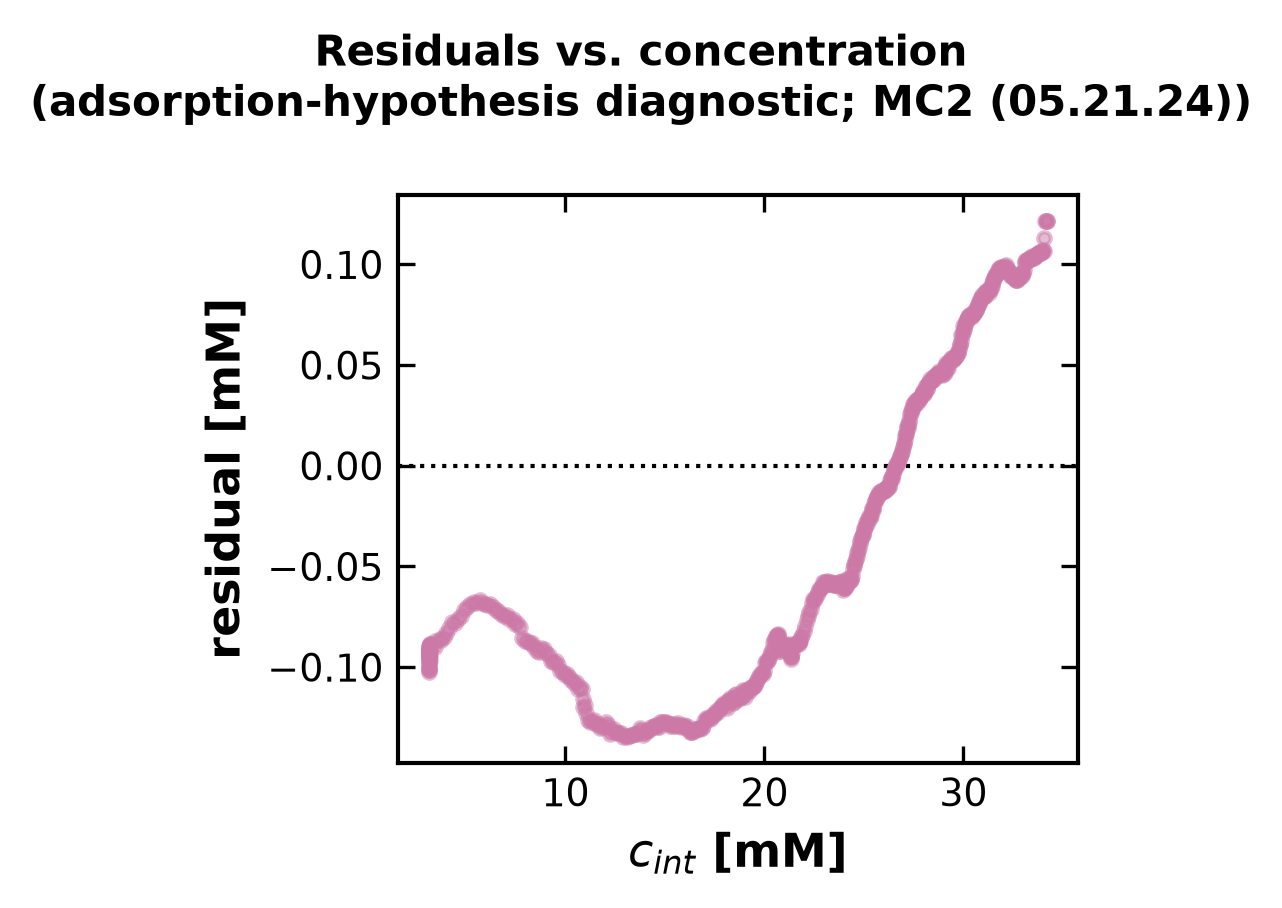
\includegraphics[width=0.49\linewidth]{figures/lacl3_residuals_vs_conc.png}\hfill
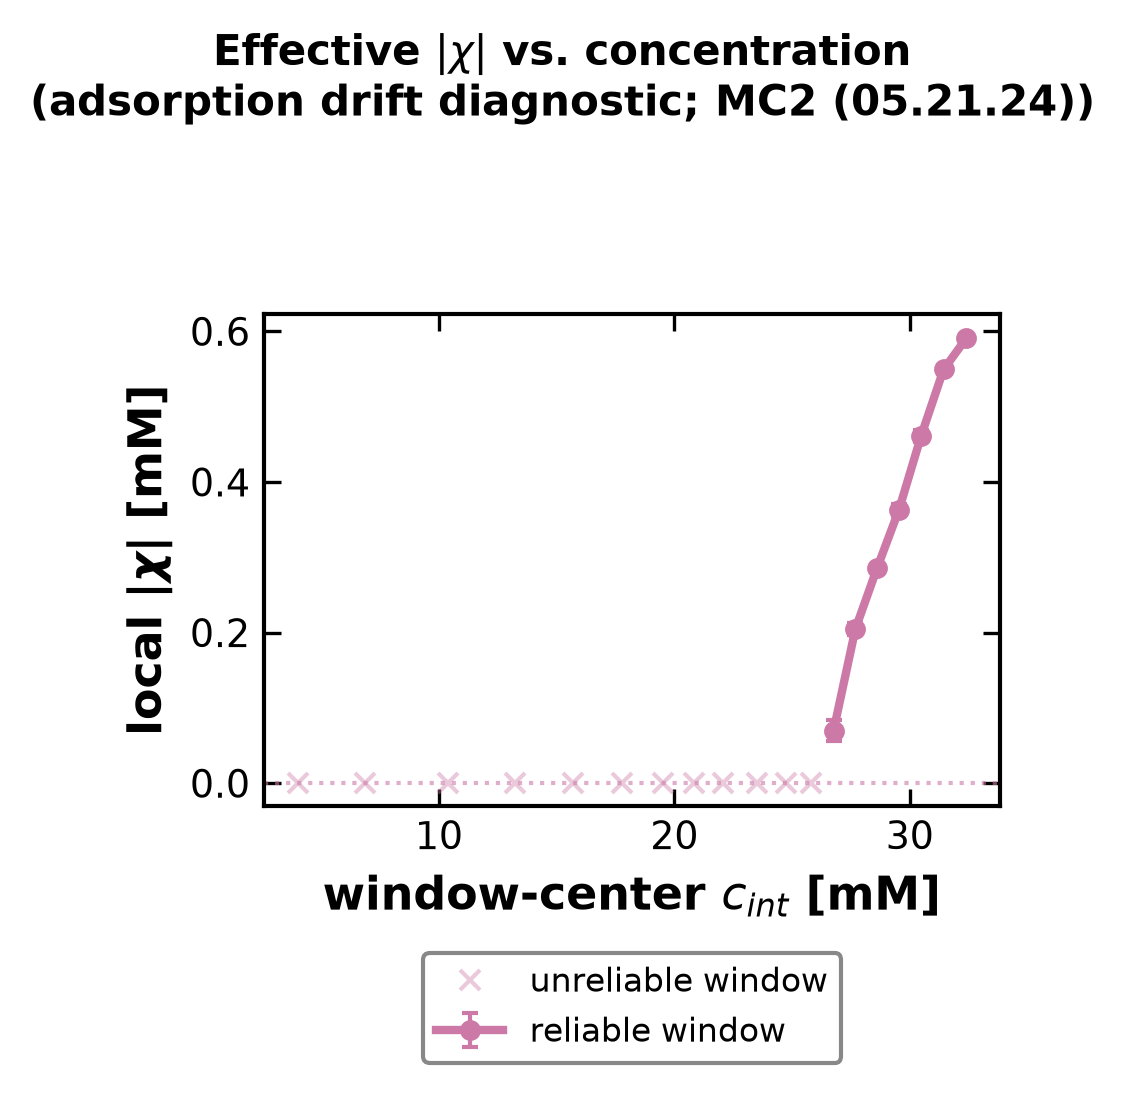
\includegraphics[width=0.49\linewidth]{figures/lacl3_effective_chi_vs_conc.png}
\caption{\textbf{Left:} residuals vs.\ $\cint$ -- the key adsorption-hypothesis
diagnostic; a smooth, strongly non-random wave ($z=-24.9$). \textbf{Right:}
sliding-window local $|\chi|$ refits ($K$ fixed at the global estimate);
unreliable windows (12 of 19, mostly at low/mid $\cint$) shown as faint
$\times$ and excluded from the trend.}
\label{fig:lacl3resid}
\end{figure}

\begin{figure}[H]
\centering
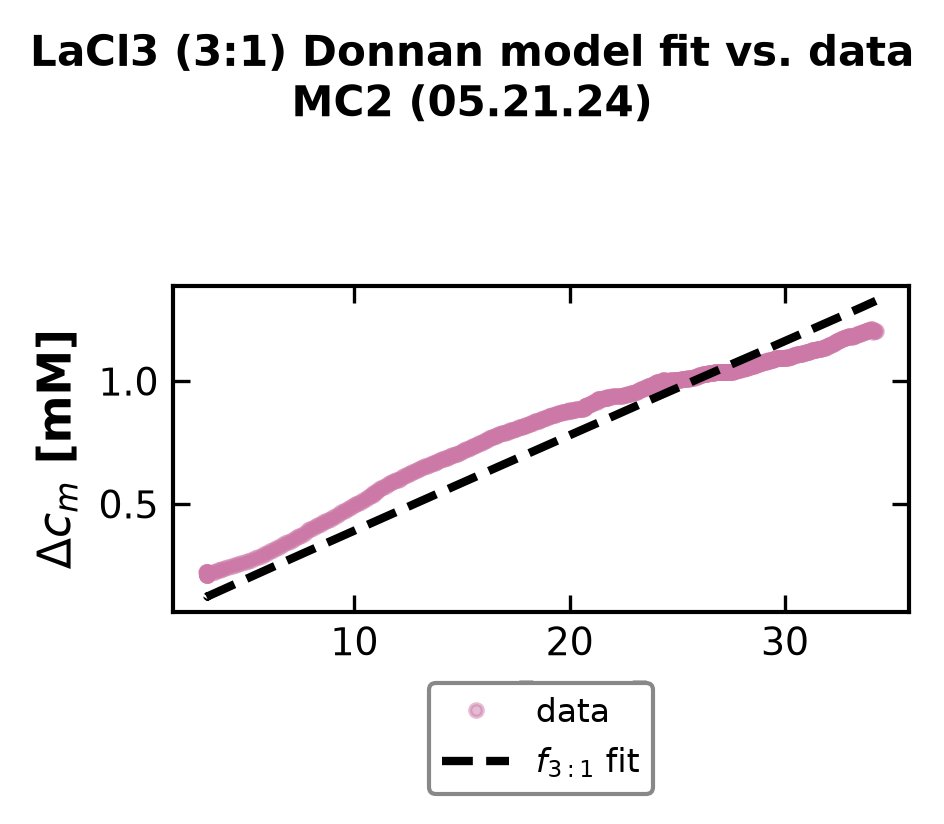
\includegraphics[width=0.49\linewidth]{figures/lacl3_fit.png}
\caption{\ce{LaCl3} corrected-model ($3{:}1$ quartic) fit vs.\ data, MC2
(05.21.24). The data's S-shaped curvature versus the fit's near-linear trend
(a consequence of $|\chi|\to0$, leaving only the $K$-scaling term) is exactly
the residual structure quantified in Figure~\ref{fig:lacl3resid}.}
\label{fig:lacl3fit}
\end{figure}

\paragraph{Comparison across salts and verdict.} $|\chi|\to0$ was already
\ce{CaCl2}'s headline finding for two of three datasets (\S\ref{sec:cacl2diag});
\ce{LaCl3} pushes this
further --- the global estimate is pinned \emph{exactly} at the $|\chi|\ge0$
bound (not just small), and only a narrow high-concentration slice of even
the local windowed estimates ever exceeds numerical noise. Fit quality
(pseudo-$R^2=0.906$, CP-corrected; was $0.803$ non-CP) is now
\emph{comparable to or better than} the \ce{CaCl2} datasets
($0.89$--$0.96$, Table~\ref{tab:cacl2all}), though the $|\chi|\to0$ pinning
itself is unchanged and remains the more extreme signature of the three
salts. \textbf{Verdict: the adsorption hypothesis extends to
\ce{La^{3+}}, and more severely than for \ce{Ca^{2+}} --- and this survives
CP.} The trend NaCl
(well-identified, nonzero $|\chi|\approx\SI{57}{mM}$, no adsorption signature) $\to$ \ce{CaCl2} ($|\chi|\to0$ for two
of three datasets, small but nonzero for the widest-range one, moderate
residual structure) $\to$ \ce{LaCl3} ($|\chi|$ pinned at exactly
$0$, strongest residual structure of the three) tracks
increasing cation charge/adsorption affinity, as expected physically.
\textbf{Critical caveat for this trend:} \ce{LaCl3}'s $|\chi|\to0$ is
\emph{confounded} with its narrow $2$--\SI{28}{mM} range and low
\ce{La^{3+}} rejection (weak identifiability, \S\ref{sec:lacl3impl}) --
whereas \ce{CaCl2}'s $|\chi|\to0$ came from \emph{wide}-range data
($\to\SI{108}{mM}$, Table~\ref{tab:cacl2data}). The NaCl$\to$\ce{CaCl2}
adsorption trend therefore rests firmly on two wide-range comparisons
(NaCl $|\chi|\approx\SI{57}{mM}$ vs.\ \ce{CaCl2} mostly $\to0$); the \ce{LaCl3}
point is \emph{consistent but range-confounded} --- a single narrow-range
dataset with no repeat (the raw-only MC4 \texttt{SLaCl3} run is future
work) --- so it should be read as \emph{suggestive, not confirmatory} of
the trend continuing to $3{:}1$. (The monotonic, not inverted-U, shape of
\ce{LaCl3}'s effective-$\chi$ drift is plausibly explained by the same
range effect: a $2$--\SI{28}{mM} window samples only the low-$\cint$
\emph{rising leg} that \ce{CaCl2} also shows at low concentration,
\S\ref{sec:cacl2diag}, not the full rise-then-fall.) A wider-range
\ce{LaCl3} dataset would strengthen the conclusion; both the
nonlinear-constraint approach and these diagnostics carry directly into
the eventual multicomponent extension.

% ############################################################
\section{Copolymer membranes: a non-adsorbing-salt control (\ce{NaCl} vs.\ \ce{Na2SO4})}\label{sec:copolymer}
% ############################################################
\S\ref{sec:cacl2}--\ref{sec:lacl3} found $|\chi|$ pinned toward zero and
systematic residual drift for \ce{Ca^{2+}} and \ce{La^{3+}} co-ions --- read
as an \emph{adsorption} signature, since the constant-charge Donnan model has
no other way to represent a concentration-dependent effective membrane
charge. This section applies the same pipeline to a different membrane
chemistry (Estrada's COOH-functionalized copolymer membranes,
\cite{estrada2026spacerarm}) and, critically, to \textbf{\ce{Na2SO4}}, a salt
whose counter-ion is \ce{Na+} --- the \emph{same} weakly-adsorbing cation as
plain \ce{NaCl}, but paired with a \emph{divalent co-ion} (\ce{SO4^{2-}})
instead of \ce{Cl-}. If the drift seen for \ce{CaCl2}/\ce{LaCl3} really is a
counter-ion-adsorption effect, \ce{Na2SO4} should behave like a
\textbf{non-adsorbing-salt positive control}: flat, well-identified $|\chi|$
with no concentration trend, on the same footing as \ce{NaCl}. The chi-spline
work of \S\ref{sec:chispline} skipped for this section, per scope.

\textbf{Headline result, stated honestly up front: the control is mixed, not
clean.} Only one of the four datasets (PEG0.1-\ce{Na2SO4}) shows the expected
flat signature; the other three show drift, weak parameter identifiability,
or both. \S\ref{sec:copolymerdiag} works through why, and
\S\ref{sec:copolymerrefine} lists concrete ways to sharpen this control in
future work.

\subsection{Model, datasets, and implementation}\label{sec:copolymerimpl}
\paragraph{Co-ion and stoichiometry.} \ce{NaCl} reuses the $1{:}1$ model of
\S\ref{sec:nacl} unmodified (co-ion $=\ce{Cl-}$, $\cs{\co}=c_{\ce{NaCl}}$).
For \ce{Na2SO4}, the co-ion is \ce{SO4^{2-}} (divalent) and the counter-ion
\ce{Na+} (monovalent) --- the \textbf{reverse} valence pairing from
\ce{CaCl2}, where the divalent species is the \emph{counter}-ion. Stoichiometry
gives $\cs{\co}=c_{\ce{Na2SO4}}$ directly (one \ce{SO4^{2-}} per formula unit,
unlike \ce{CaCl2}'s $\cs{\co}=2c$).

\paragraph{Governing equation: the $1{:}2$ co-ion cubic.} Following the same
electroneutrality construction as \eqref{eq:11co}--\eqref{eq:31co} but for a
divalent co-ion against a monovalent counter-ion, the membrane co-ion
concentration solves
\begin{equation}
  \cm{\co}^3 + |\chi|\,\cm{\co}^2 + \tfrac14|\chi|^2\,\cm{\co} - K\,\cs{\co}^3 = 0,
  \qquad \text{prediction} = \cm{\co}(\cint) - \cm{\co}(\cp),
  \label{eq:na2so4model}
\end{equation}
with $K\ge0$ again a lumped constant absorbing $\dstar$ and stoichiometric
factors. \textbf{This cubic differs from \ce{CaCl2}'s} \eqref{eq:cacl2model}
by the extra linear term $\tfrac14|\chi|^2\cm{\co}$ --- a direct consequence
of squaring the divalent co-ion's electroneutrality exponent rather than the
counter-ion's; \eqref{eq:cacl2model} has no such term because there the
divalent species is the counter-ion, which enters differently. \note{Confirm
this $1{:}2$ non-ideal factor split ($\dstar$ vs.\ a possible additional
$\delta^{\circ}_{\co}$ factor) with the group, as for the $2{:}1$/$3{:}1$
cases -- \S\ref{sec:donnan}.}

\paragraph{Root-solve implementation.} $g(t) \coloneqq t^3+|\chi|t^2+
\tfrac14|\chi|^2 t - K\cs{\co}^3$ has $g'(t)=3t^2+2|\chi|t+\tfrac14|\chi|^2$,
a quadratic in $t$ with discriminant $(2|\chi|)^2-4\cdot3\cdot\tfrac14|\chi|^2
=|\chi|^2\ge0$ and roots $t=-|\chi|/6,\,-|\chi|/2$ --- \textbf{both $\le0$ for
$|\chi|\ge0$} --- so $g$ is strictly increasing on $t\ge0$ for any physical
$|\chi|$, and a simple vectorized bisection on $[0,\text{expanding bracket}]$
is both correct and well-conditioned (no Cardano branch needed, unlike
\ce{CaCl2}'s cubic, where Cardano was used purely for speed). Verified
against \texttt{numpy.roots} on a 200-point random parameter scan: maximum
relative cubic residual $5.81\times10^{-16}$, maximum relative error vs.\
\texttt{numpy.roots} $8.87\times10^{-16}$.

\paragraph{Membrane diffusivities.} Solution-phase ambipolar diffusivities
(Nernst--Hartley, as elsewhere in this report) are converted to
\textbf{membrane-phase} diffusivities via the Mackie--Meares relation,
$D_{\mathrm m}=D_{\mathrm s}\big(\phi_{\mathrm w}/(2-\phi_{\mathrm w})\big)^2$,
using each membrane's water volume fraction $\phi_{\mathrm w}$ from the SI
(Section~S5/Table~S3, \cite{estrada2026spacerarm}). $\ell=\SI{80}{nm}$ is
\textbf{assumed} for all four datasets (mirroring \ce{CaCl2}/\ce{LaCl3}; not
reported in the SI for \emph{any} of these membranes).

\paragraph{Datasets and provenance caveats.}
\begin{table}[H]
\centering\small
\begin{tabular}{llrcc}
\toprule
Dataset & Salt & $n$ & $\phi_{\mathrm w}$ & $|\chi|_{\zeta}$ (SI) \\
\midrule
PEG0.1-\ce{NaCl}   & \ce{NaCl}   & 1777 & $0.41$ (PEG0)         & $\SI{12.60}{mM}$ (pH 6.08) \\
PEG6.5-\ce{NaCl}   & \ce{NaCl}   & 2410 & $0.51$ (PEG4, \emph{proxy}) & none in SI \\
PEG0.1-\ce{Na2SO4} & \ce{Na2SO4} & 1772 & $0.41$ (PEG0)         & $\SI{12.60}{mM}$ (pH 6.08) \\
ALK1.2-\ce{Na2SO4} & \ce{Na2SO4} & 2882 & $0.06$ (ALK1)         & none in SI \\
\bottomrule
\end{tabular}
\caption{The four focus datasets (\texttt{docs/prompts/copolymer\_nacl\_na2so4.md}),
all unadjusted pH~6. \textbf{PEG6.5 has neither an SI $\phi_{\mathrm w}$ nor
an SI zeta-potential $\chi$} of its own -- the SI (\cite{estrada2026spacerarm})
only characterizes Azide/PEG0/PEG10 for $\chi$ and Azide/PEG0/PEG4/ALK1 for
$\phi_{\mathrm w}$, a genuine gap in the source data, not a processing choice.
PEG6.5's $\phi_{\mathrm w}$ uses PEG4's value as a \textbf{proxy}, flagged
throughout.}
\label{tab:copolymerdata}
\end{table}
\textbf{ALK1.2-\ce{Na2SO4} calibration.} Its raw campaign sheet has \emph{no}
per-vial conductivity at all (every vial's \texttt{cond} cell is blank in the
source workbook) -- the standard vial-conductivity calibration
(\S\ref{sec:preproc}) is unavailable. As a fallback, the calibration is
derived directly from the \emph{processed} sheet's own $\cint$-vs-$\kappa_{\mathrm r}$
relationship (linear regression, $R^2=0.9984$, $n=3101$), used in place of
the usual vial-based fit. \textbf{CP status:} the $\cint/\kappa_{\mathrm r}$
coefficient-of-variation diagnostic (\S\ref{sec:preproc}) gives
$0.0198$--$0.0328$ for all four processed sheets, in the same
bulk/non-CP cluster as the NF270 non-CP sheets (vs.\ $\approx0.25$ for an
already-CP-corrected sheet) -- CP is applied on top, as for the other
salt sections.

\subsection{Results}\label{sec:copolymerresults}
\begin{table}[H]
\centering\small\setlength{\tabcolsep}{4pt}
\begin{tabular}{lrccccc}
\toprule
Dataset & $n$ & $|\chi|$ [\si{mM}] (95\% CI) & $K$ (95\% CI) & SSE & pseudo-$R^2$ & MS \% \\
\midrule
PEG0.1-\ce{NaCl}   & 1777 & $24.94\ (8.54,\,232.8)$ & $0.00195\ (0.00070,\,0.0179)$ & $0.387$ & $0.793$ & $61\%$ \\
PEG6.5-\ce{NaCl}   & 2410 & $6148\ (13741,\,550625)$ & $0.351\ (0.761,\,5.41)$ & $0.339$ & $0.539$ & $72\%$ \\
PEG0.1-\ce{Na2SO4} & 1772 & $1.349\ (1.178,\,1.553)$ & $2.0\times10^{-7}$ (see note) & $0.792$ & $0.790$ & $72\%$ \\
ALK1.2-\ce{Na2SO4} & 2882 & $50.93\ (45.24,\,57.89)$ & $0.0176\ (0.0148,\,0.0217)$ & $1870.7$ & $0.763$ & $100\%$ \\
\bottomrule
\end{tabular}
\caption{Copolymer regression, all four datasets, CP-corrected, bounded
model (\eqref{eq:na2so4model} for \ce{Na2SO4}, the standard corrected $1{:}1$
model for \ce{NaCl}); 95\% CIs are profile-likelihood, MS = multi-start \%
reaching the global optimum (100 random starts). \textbf{PEG6.5-\ce{NaCl}'s
CI is inverted (lower bound above the point estimate) because the profile
likelihood is essentially flat}: \S\ref{sec:copolymerdiag} confirms directly
that SSE changes by $<1\%$ over a $500\times$ range in $|\chi|$, so the
reported CI bounds are an artifact of where the $F$-test threshold happens to
cross a near-flat curve, not a meaningful interval. \textbf{PEG0.1-\ce{Na2SO4}'s
$K$} is pinned near zero ($2\times10^{-7}$) and its profile-likelihood search
returns a degenerate (non-bracketing) interval at that boundary -- read as
``$K$ unidentifiably close to zero,'' the same boundary pathology
\S\ref{sec:lacl3results} reports for \ce{LaCl3}'s $|\chi|$, not a
computational error.}
\label{tab:copolymerall}
\end{table}

\begin{figure}[H]
\centering
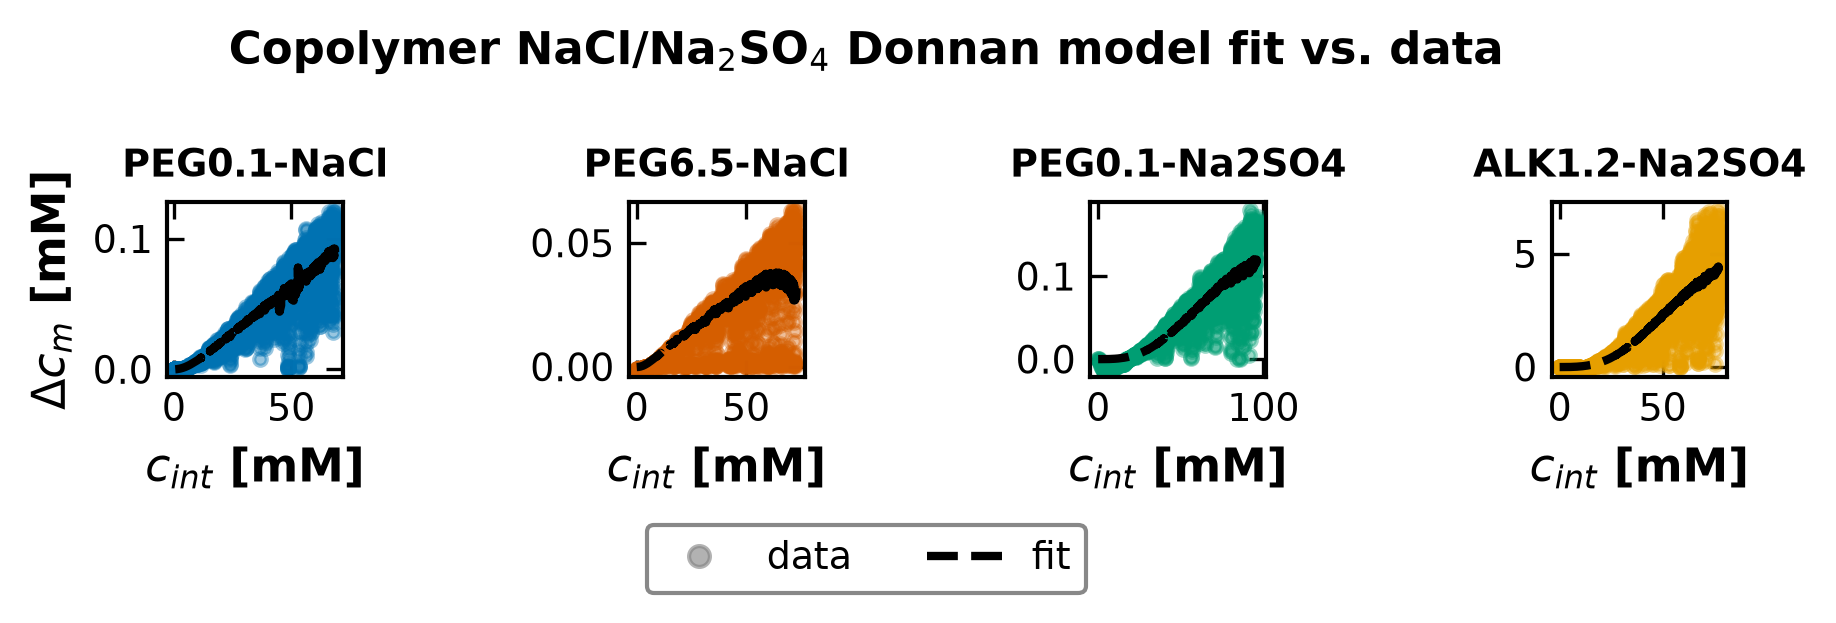
\includegraphics[width=\linewidth]{figures/copolymer_fits.png}
\caption{Copolymer model fit vs.\ data, by dataset. \ce{Na2SO4} uses the
$1{:}2$ cubic \eqref{eq:na2so4model}; \ce{NaCl} the standard corrected
$1{:}1$ model.}
\label{fig:copolymerfits}
\end{figure}

\begin{figure}[H]
\centering
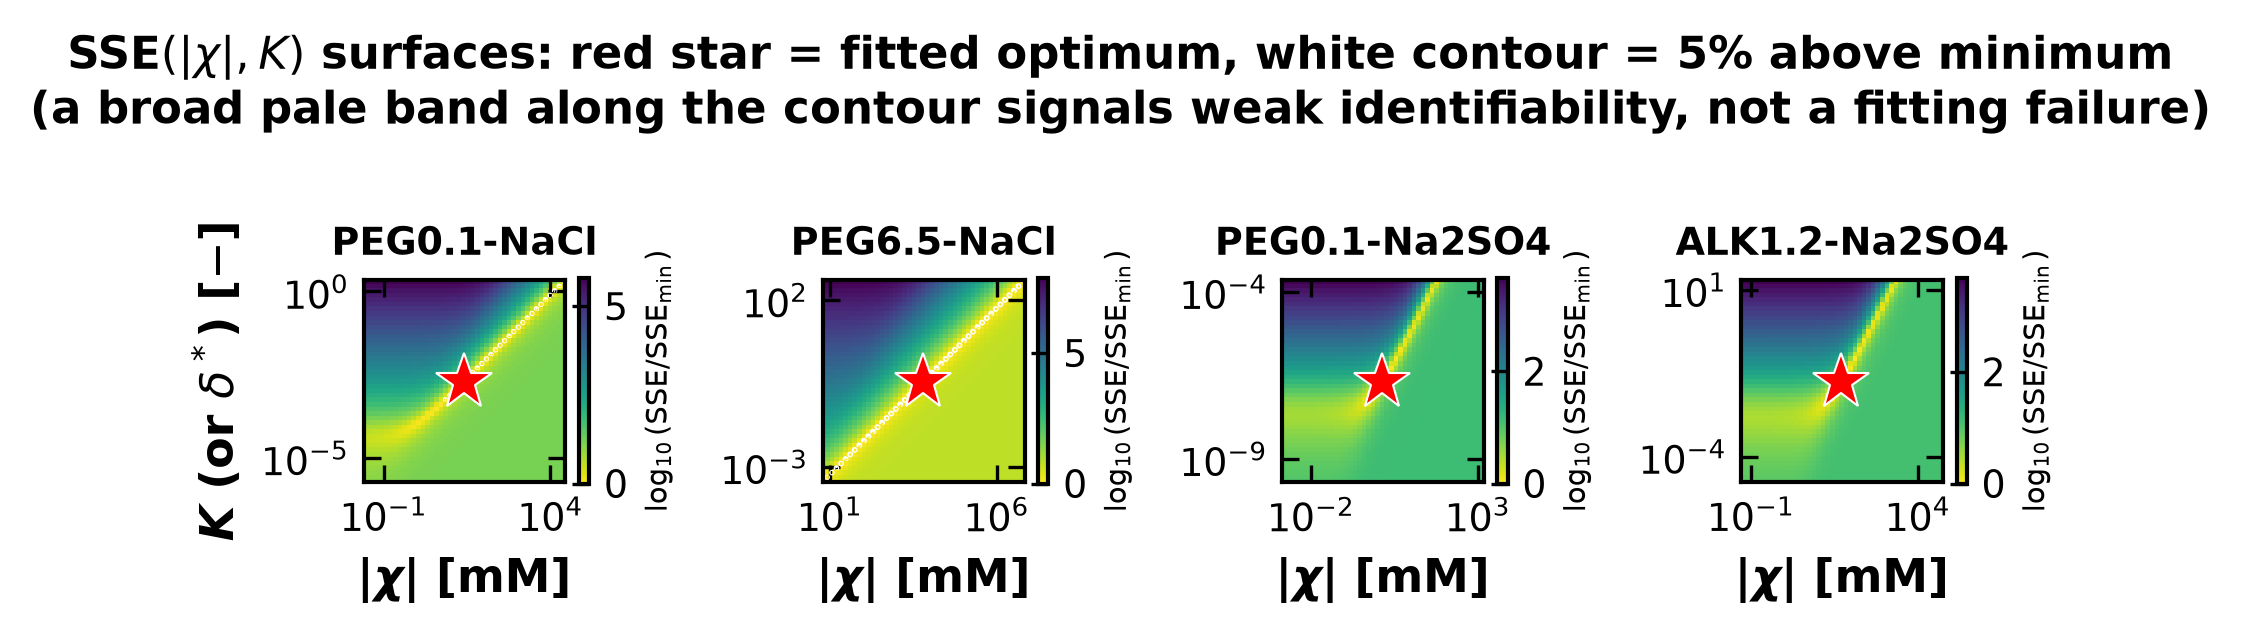
\includegraphics[width=\linewidth]{figures/copolymer_sse_heatmaps.png}
\caption{$\SSE(|\chi|,K)$ surfaces (log-log axes, both parameters fixed at
each grid point -- \emph{not} a profile likelihood): red star = fitted
optimum, white contour = 5\% above the minimum SSE. PEG0.1-\ce{NaCl} and
especially PEG6.5-\ce{NaCl} show the 5\% contour running the \emph{full width}
of a wide search window -- a long, shallow ridge along which $|\chi|$ and $K$
trade off with almost no SSE cost, i.e.\ the data pin down some combination
of the two parameters but not each individually. PEG0.1-\ce{Na2SO4} and
ALK1.2-\ce{Na2SO4} show a visibly more localized bowl -- better, though still
imperfect, joint identifiability. This is the direct visual counterpart of
the numeric CIs in Table~\ref{tab:copolymerall}.}
\label{fig:copolymerheatmaps}
\end{figure}

\subsection{Validation against independent zeta-potential $|\chi|$}\label{sec:copolymerzeta}
Only PEG0 (used by both PEG0.1 datasets) has an SI zeta-potential $\chi$ at
pH~6.08 ($\SI{12.60}{mM}$); PEG6/ALK1 were not zeta-characterized in the SI
(Table~\ref{tab:copolymerdata}). \textbf{The two PEG0.1 salts disagree with
the SI value in \emph{opposite} directions}: PEG0.1-\ce{NaCl} regresses
$\approx2\times$ \emph{higher} ($\SI{24.9}{mM}$ vs.\ $\SI{12.6}{mM}$) while
PEG0.1-\ce{Na2SO4} regresses $\approx9\times$ \emph{lower} ($\SI{1.35}{mM}$
vs.\ $\SI{12.6}{mM}$) than the same independent reference value, on the same
membrane. Since the two salts share a membrane but not a co-ion valence, this
is consistent with the lumped constant $K$ (which differs by co-ion physics,
\eqref{eq:cacl2model} vs.\ \eqref{eq:na2so4model}) absorbing model-form error
that a single constant-$\chi$ Donnan fit cannot separate out -- the same
absolute-scale caveat already flagged for the lumped $K$ throughout
\S\ref{sec:cacl2}--\ref{sec:lacl3}.

\begin{figure}[H]
\centering
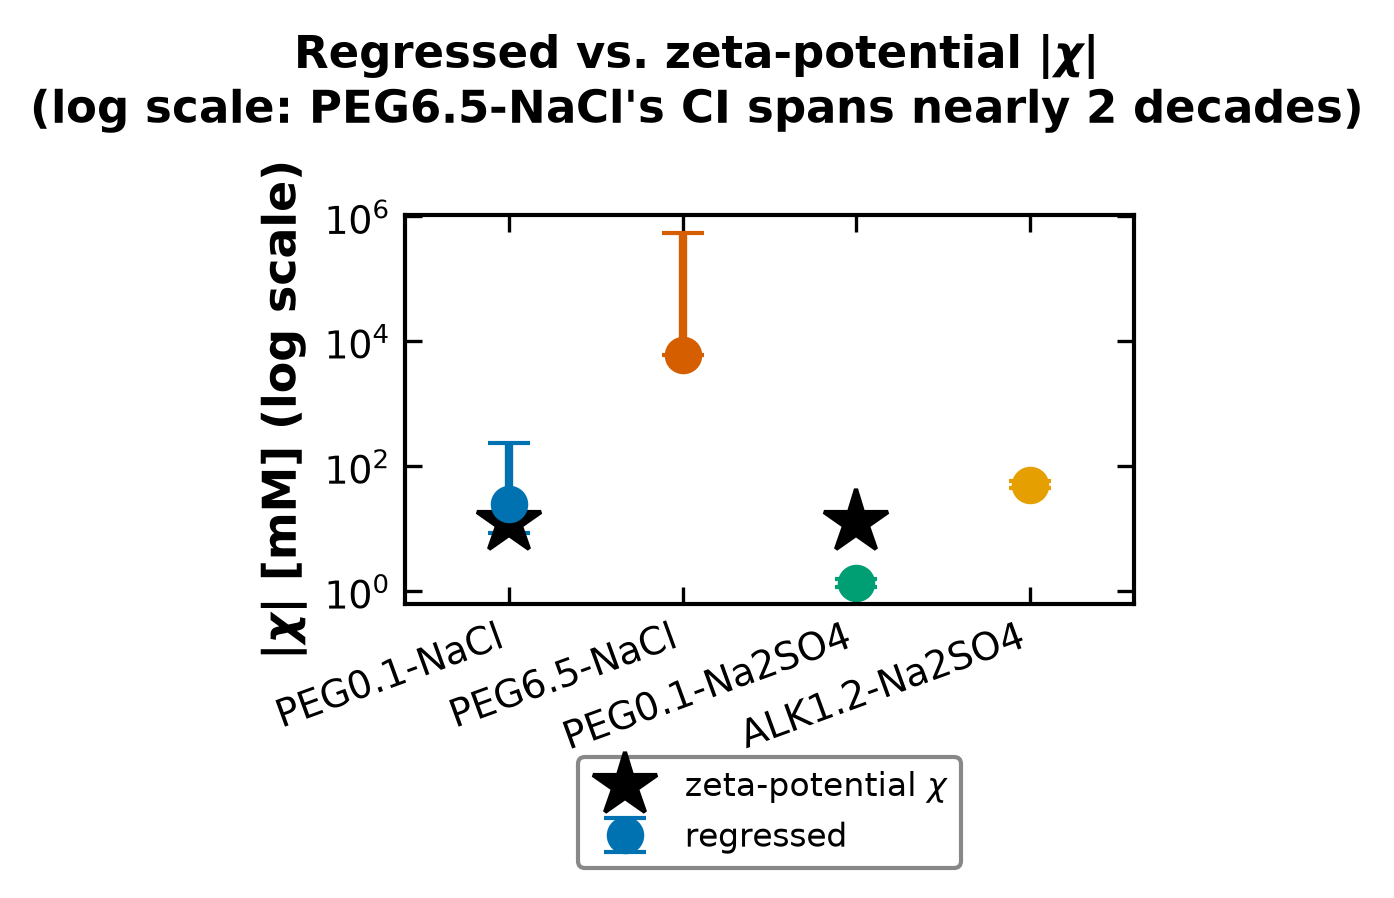
\includegraphics[width=0.55\linewidth]{figures/copolymer_zeta_validation.png}
\caption{Regressed $|\chi|$ (95\% profile-likelihood CI) vs.\ independent
SI zeta-potential $\chi$ (black stars), log-scale $y$-axis (the four point
estimates and CIs span nearly six orders of magnitude). PEG6.5-\ce{NaCl} and
ALK1.2-\ce{Na2SO4} have no SI $\chi$ to compare against.}
\label{fig:copolymerzeta}
\end{figure}

\subsection{Adsorption-hypothesis diagnostics: a mixed result}\label{sec:copolymerdiag}
\paragraph{PEG0.1-\ce{Na2SO4}: the one clean control.} Sliding-window
effective $|\chi|$ is essentially \textbf{flat} across the full concentration
range (43 windows, 40 reliable, range $[1.21,1.84]$\,mM, slope
$+0.0005$\,mM/mM -- indistinguishable from zero) -- exactly the
non-adsorbing-salt signature this control was designed to find. Fit quality
is comparable to the other datasets (pseudo-$R^2=0.790$), and multi-start
convergence is $72\%$.

\paragraph{The other three datasets do not confirm the control cleanly.}
\begin{itemize}
  \item \textbf{PEG0.1-\ce{NaCl}} \emph{drifts}: 43/43 reliable windows,
  local $|\chi|$ rising from $\SI{20.5}{mM}$ to $\SI{199.9}{mM}$
  (slope $-0.55$\,mM/mM in the fitted direction -- concentration-dependent,
  not flat), on the \emph{same} weakly-adsorbing \ce{Na+} counter-ion that
  \S\ref{sec:nacl}'s NF270 \ce{NaCl} data showed \emph{no} such drift for.
  \item \textbf{ALK1.2-\ce{Na2SO4}} also \emph{drifts}: 71 windows (67
  reliable), local $|\chi|$ from $\SI{42.9}{mM}$ to $\SI{120.9}{mM}$,
  despite sharing \ce{Na2SO4}'s co-ion with the clean PEG0.1-\ce{Na2SO4}
  case -- so the drift here tracks with \emph{membrane} (ALK1.2 vs.\ PEG0.1),
  not salt identity.
  \item \textbf{PEG6.5-\ce{NaCl}} is not merely drifting but \textbf{weakly
  identified}: 0 of 59 sliding windows converge reliably, and a direct
  SSE-profile check (fixing $|\chi|$ across
  $\{0.1,1,5,10,24.9,50,100,500,1000,6147,50000\}$\,mM and re-optimizing $K$
  each time) shows SSE changes by \textbf{$<1\%$ over a $500\times$ range in
  $|\chi|$} -- confirmed as a genuine flat ridge in the SSE surface
  (Figure~\ref{fig:copolymerheatmaps}), not an optimizer failure. This
  dataset's very low pseudo-$R^2$ ($0.539$) and inverted CI
  (Table~\ref{tab:copolymerall}) are symptoms of the same underlying
  non-identifiability.
\end{itemize}
\textbf{Residual sign-runs are non-random for all four} (PEG0.1-\ce{NaCl}
$z=-14.3$; PEG6.5-\ce{NaCl} $z=-28.4$; PEG0.1-\ce{Na2SO4} $z=-10.3$;
ALK1.2-\ce{Na2SO4} $z=-9.2$; $n=587,500,670,1196$ runs respectively) -- even
PEG0.1-\ce{Na2SO4}'s residuals show short-range non-random structure by this
test. The distinguishing diagnostic between the "clean" and "messy" cases is
therefore not the sign-runs test alone, but the \emph{sliding-window trend}:
flat-with-concentration (PEG0.1-\ce{Na2SO4}) vs.\ systematically drifting
(the other three).

\begin{figure}[H]
\centering
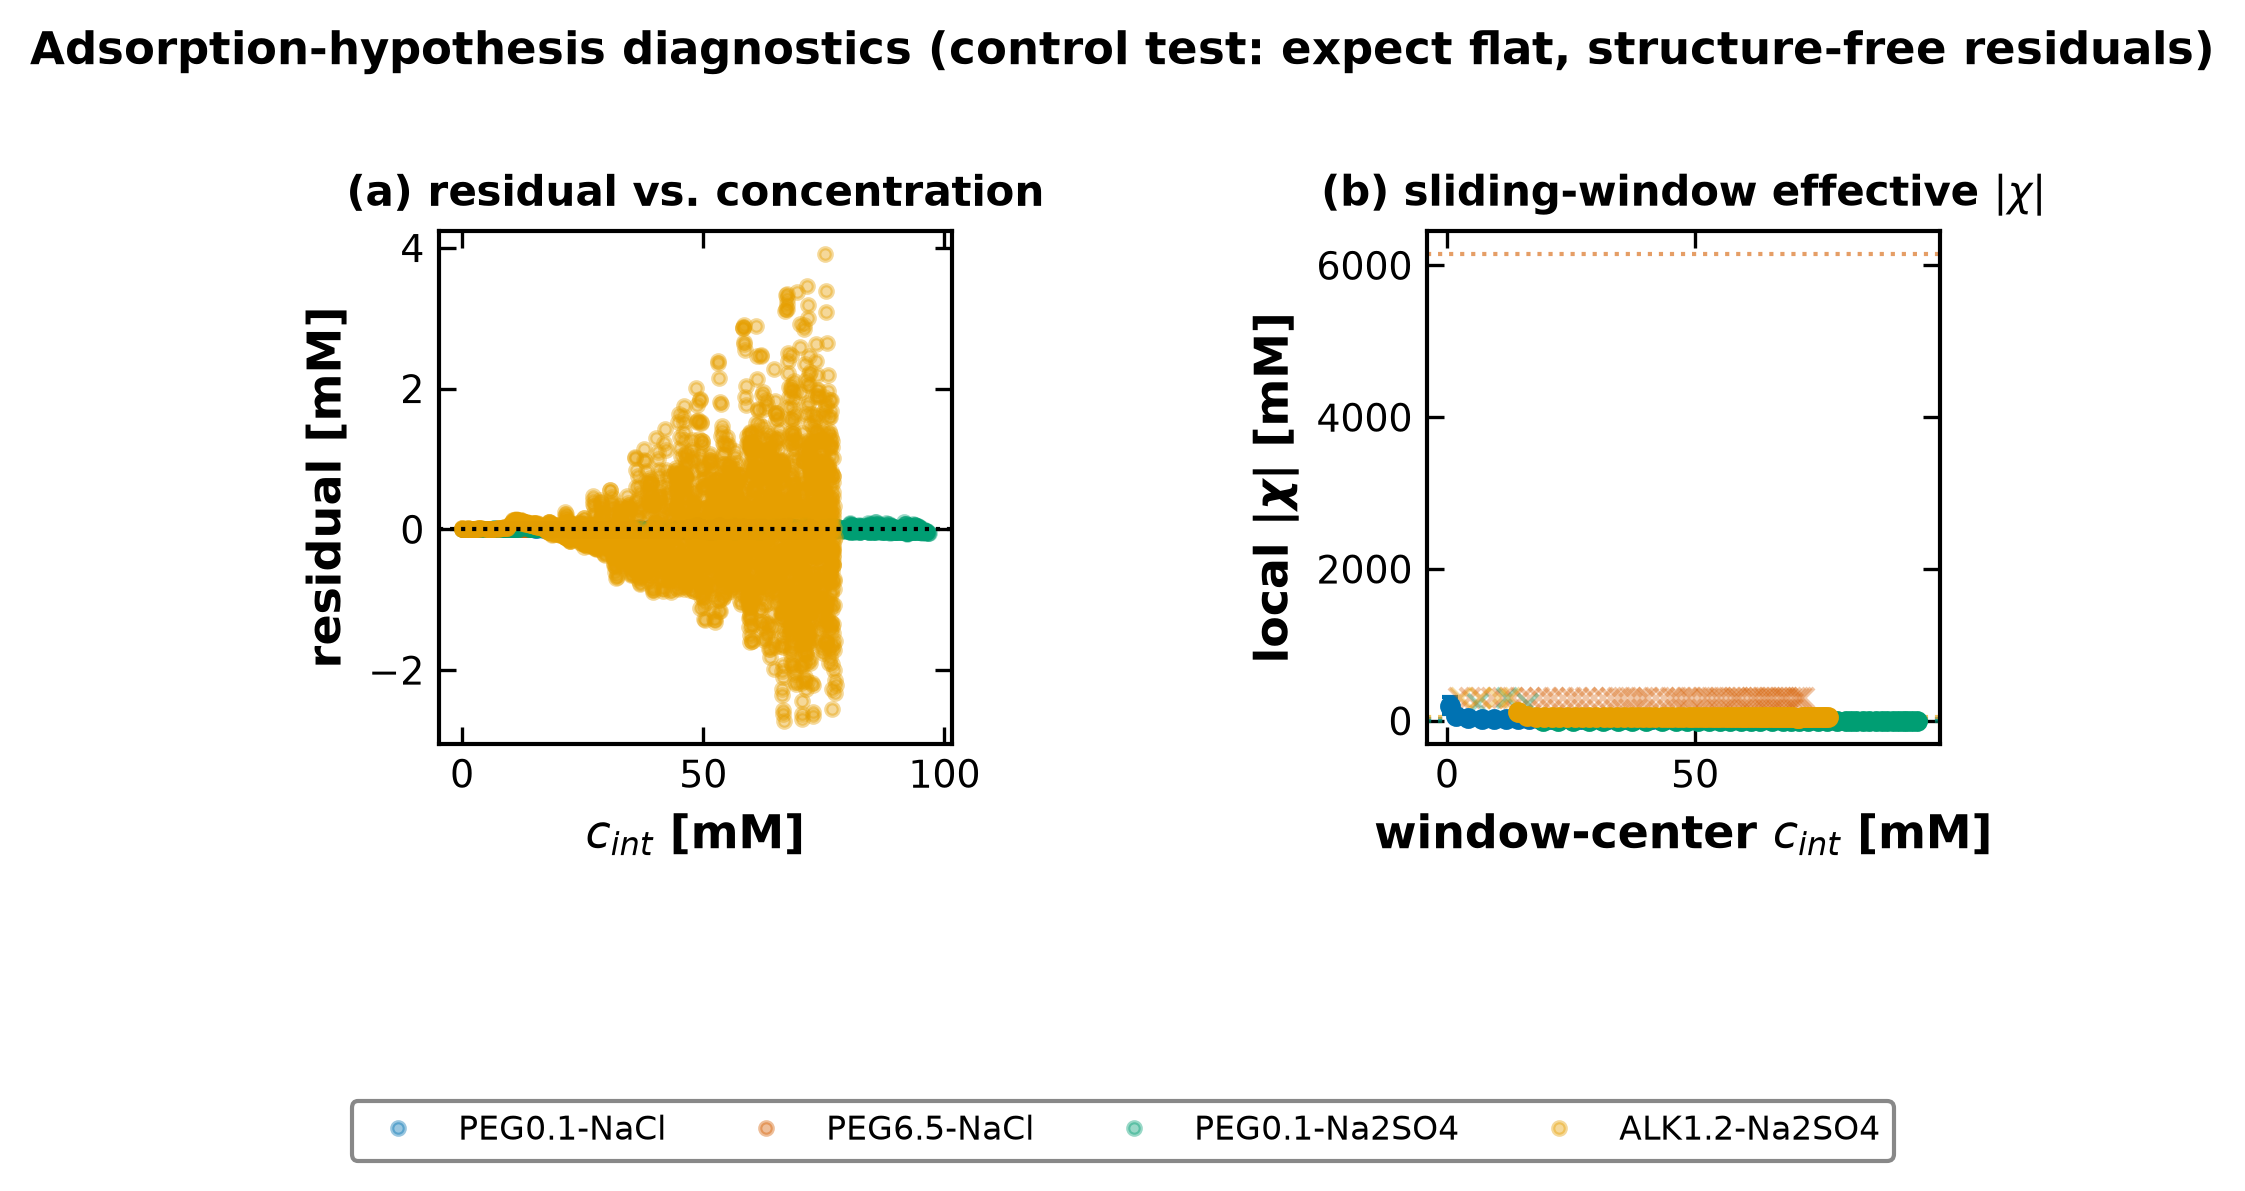
\includegraphics[width=\linewidth]{figures/copolymer_adsorption_diagnostics.png}
\caption{(a) residual vs.\ $\cint$; PEG6.5-\ce{NaCl} omitted from the trend
panel (0/59 reliable windows) but included in the legend and panel (a).
(b) sliding-window effective $|\chi|(\cint)$; unreliable windows shown as
faint $\times$. PEG0.1-\ce{Na2SO4}'s near-flat trend (green) contrasts with
PEG0.1-\ce{NaCl} and ALK1.2-\ce{Na2SO4}'s visible rise.}
\label{fig:copolymerdiag}
\end{figure}

\paragraph{AR(1) autocorrelation.} All four datasets show
near-unit-root Cochrane--Orcutt $\hat\phi$ ($0.967$--$0.999$), the same
severe-non-stationarity pattern documented for NaCl's raw measurements
(\S\ref{sec:naclAR1}) and inherited here rather than newly discovered. The
resulting whitened-vs-i.i.d.\ Wald interval fold factors are large and
inconsistent across datasets ($649\times$, $0.23\times$, $36\times$,
$69\times$ for PEG0.1-\ce{NaCl}, PEG6.5-\ce{NaCl}, PEG0.1-\ce{Na2SO4},
ALK1.2-\ce{Na2SO4} respectively) -- PEG6.5-\ce{NaCl}'s near-$1\times$ fold is
itself diagnostic: whitening barely changes an already-uninformative interval
on a flat ridge.

\begin{figure}[H]
\centering
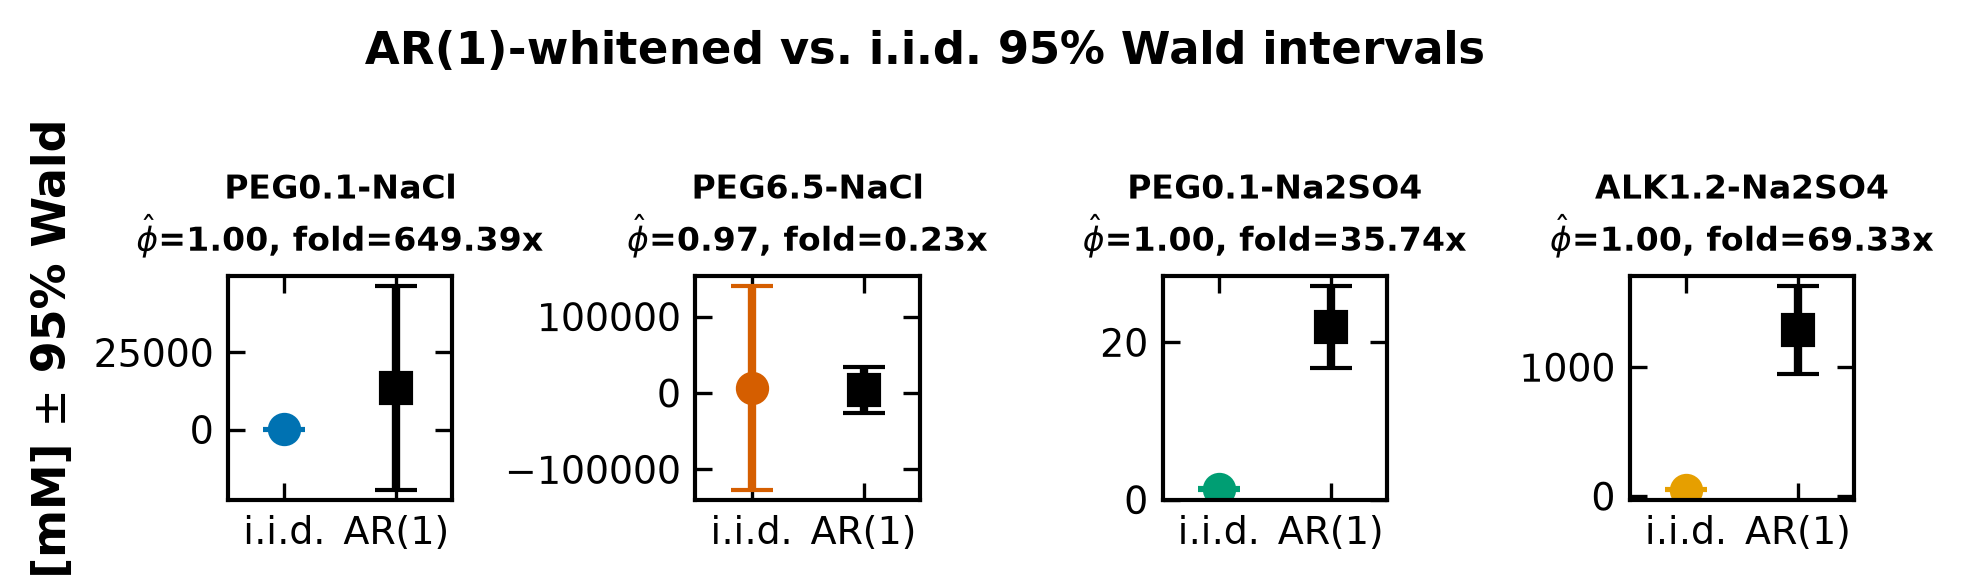
\includegraphics[width=\linewidth]{figures/copolymer_ar1.png}
\caption{AR(1)-whitened vs.\ i.i.d.\ 95\% Wald intervals for $|\chi|$, all
four datasets. Near-unit-root $\hat\phi$ throughout (as in
\S\ref{sec:naclAR1}) means the i.i.d.\ interval badly understates true
uncertainty for three of the four datasets.}
\label{fig:copolymerar1}
\end{figure}

\paragraph{Verdict.} \textbf{The \ce{Na2SO4} non-adsorbing-salt control is
only partially confirmed.} PEG0.1-\ce{Na2SO4} behaves exactly as hypothesized
(flat effective $|\chi|$, no concentration trend). But PEG0.1-\ce{NaCl} --
the same membrane, same counter-ion family as plain \ce{NaCl} -- drifts,
which the working hypothesis (drift $=$ counter-ion adsorption) does
\emph{not} predict for \ce{Na+}; and ALK1.2-\ce{Na2SO4} drifts despite
sharing PEG0.1-\ce{Na2SO4}'s salt. The cleanest reading is that
\textbf{membrane chemistry/geometry (via the assumed-constant $\ell$,
$\phi_{\mathrm w}$, or genuine membrane-specific effects) confounds the
salt-identity comparison this control was meant to isolate}, and PEG6.5-\ce{NaCl}'s
extreme non-identifiability further limits what can be concluded from a
single narrow four-dataset set. This should be read as an honest, mixed
result -- not a clean confirmation or refutation of the adsorption
hypothesis -- pending the refinements of \S\ref{sec:copolymerrefine}.

\subsection{The noise question: other, unanalyzed copolymer runs}\label{sec:copolymernoise}
Laurianne raised a separate methodological question about \textbf{other}
copolymer runs not analyzed in this section (e.g.\ \texttt{ALK1.1
10.16.24NaCl}), which are visibly noisier than the four focus datasets here.
\note{Recommendation, not yet implemented: (i) a \textbf{robust loss}
(Huber or soft-L1, via \texttt{scipy.optimize.least\_squares}'s built-in
\texttt{loss=} argument -- a one-line change, no new machinery) would
down-weight isolated outlier points without discarding them outright; (ii) a
\textbf{rolling-median (Hampel) prefilter} on the raw conductivity signal,
applied \emph{before} calibration (\S\ref{sec:preproc}), would catch
transient spikes (air bubbles, vial swaps) that a single robust-loss fit
cannot fully absorb if they cluster in time; (iii) flagging such transients
explicitly (e.g.\ from large single-point jumps in raw $\kappa$) is cheap
and auditable, versus silently down-weighting everything; (iv) the AR(1)
correction already in this pipeline (\S\ref{sec:copolymerdiag}) partially
compensates for correlated noise, but was designed for autocorrelation, not
outlier rejection, and should not be treated as a substitute for (i)--(iii).
This is scoped as future work for the noisier runs Laurianne flagged, not a
change to the four datasets analyzed here.}

\subsection{Recommended refinements to this analysis}\label{sec:copolymerrefine}
\begin{itemize}
  \item \textbf{Measure $\phi_{\mathrm w}$ and $\ell$ directly} for all four
  membranes rather than assuming $\ell=\SI{80}{nm}$ (unmeasured for every
  membrane in this report) and proxying PEG6.5's $\phi_{\mathrm w}$ from
  PEG4 -- both currently confound the absolute $|\chi|$/$K$ scale.
  \item \textbf{Independently validate ALK1.2-\ce{Na2SO4}'s calibration}
  beyond the processed-sheet-derived fallback (\S\ref{sec:copolymerimpl}),
  e.g.\ by re-measuring vial conductivities for that campaign if the raw
  samples still exist.
  \item \textbf{Investigate whether AR(1)/state-space noise modeling changes
  the identifiability picture}, particularly for PEG6.5-\ce{NaCl}'s flat
  ridge -- a correlated-error model could plausibly sharpen (or could
  further degrade) the effective information content of a near-unit-root
  series.
  \item \textbf{Pool multiple concentration ranges or repeat runs per
  membrane} to try to break the $|\chi|$/$K$ ridge degeneracy
  (Figure~\ref{fig:copolymerheatmaps}) -- a single run's SSE surface may be
  flat where the combination of several is not.
  \item \textbf{Verify the Mackie--Meares $\phi_{\mathrm w}\to D_{\mathrm m}$
  assumption} against literature values for these specific copolymer
  chemistries; it was carried over from the CaCl2/LaCl3 treatment without a
  copolymer-specific check.
  \item \textbf{Extend the analysis to the other, unflagged (non-noisy)
  copolymer datasets} not touched in this four-dataset scope, to see whether
  the PEG0.1-\ce{Na2SO4}-like flat signature or the drifting signature is
  more typical of this membrane family.
\end{itemize}

% ############################################################
\section{Cross-salt synthesis and discussion}\label{sec:synthesis}
% ############################################################
\S\ref{sec:nacl}--\ref{sec:lacl3} developed the NaCl, \ce{CaCl2}, and
\ce{LaCl3} analyses largely independently; this section ties the $1{:}1$/
$2{:}1$/$3{:}1$ story together and states what carries across all three,
cross-referencing rather than restating the per-salt numbers.

\subsection{The valence trend}\label{sec:valencetrend}
A constant-charge Donnan model \textbf{fails progressively for
multivalent counter-ions}:
\begin{itemize}[itemsep=2pt]
  \item \textbf{NaCl ($1{:}1$, \S\ref{sec:reproMATLAB}--\ref{sec:naclUQ}):} a
        clean, well-identified fit on the primary dataset, \textbf{CP-corrected
        (primary, \S\ref{sec:naclUQ}), $|\chi|\approx\SI{56.74}{mM}$},
        $\dstar\approx0.2049$ (non-CP: $\SI{50.36}{mM}$, $0.3263$ --- same order
        of magnitude), with the
        nonlinear region visually indistinguishable from the Wald ellipse.
        Across all nine datasets (\S\ref{sec:naclAll}), the primary CP set is
        uniformly \emph{our} thin-film CP (MC2, MC5(2)$\to$``MC5 (05.27.26)'',
        and the six reconstructed runs); the lone dataset with its own
        already-applied CP
        (MC5-main, Estrada's own CP) is kept as an explicit comparison, not a primary row, since
        it disagrees with MC5(2)+our-CP by $13\%$ ($49.56$ vs.\
        $\SI{56.07}{mM}$) --- an our-CP-vs-Estrada's-CP implementation
        discrepancy (\S\ref{sec:naclAllResults}), not a non-CP-vs-CP question.
        MC2, now correctly identified as needing CP (it was mistakenly
        classified already-CP in an earlier pass), still disagrees
        cut-to-cut with MC5(2) (MC2 $|\chi|=21.42$\,mM vs.\ $\SI{56.07}{mM}$) ---
        a concentration-range
        effect
        (\S\ref{sec:crosscuts}), not evidence against the model itself.
  \item \textbf{\ce{CaCl2} ($2{:}1$, \S\ref{sec:cacl2}):} under CP, \emph{two
        of three} datasets still drive $|\chi|\to0$ ($0.0000$--$0.0494$\,mM), while
        the widest-range dataset (MC5 05.27.26) now resolves to a small but
        \emph{statistically nonzero} $|\chi|=2.95$\,mM (CI excludes zero,
        Table~\ref{tab:cacl2all}) --- still $\approx19\times$ below NaCl. All three
        show strong non-random residual structure
        (sign-runs $z=-23.1$ to $-42.3$) and effective-$\chi$ drift with
        concentration (non-monotonic, inverted-U). This remains \emph{sharper}
        than ``a smaller $\chi$ than NaCl'' --- the co-ion exclusion effect
        appears mostly masked on average, consistent with
        concentration-dependent \ce{Ca^{2+}} adsorption; CP \emph{sharpens}
        (reveals a small residual signal for one dataset) rather than
        overturns this.
  \item \textbf{\ce{LaCl3} ($3{:}1$, \S\ref{sec:lacl3}):} pushes this further
        still --- $|\chi|$ is pinned \emph{exactly} at its $\ge0$ bound (a
        boundary solution, not an interior optimum, unchanged by CP), fit quality
        \emph{improves under CP} (pseudo-$R^2=0.906$, up from $0.803$
        non-CP --- now comparable to or better than \ce{CaCl2}), and the
        residual sign-runs statistic ($z=-24.9$ on $n=623$) is the most
        extreme in the report. \textbf{But this point is range-confounded}
        (\S\ref{sec:lacl3diag}): \ce{LaCl3}'s one dataset spans only
        $2$--\SI{28}{mM}, while \ce{CaCl2}'s $|\chi|\to0$ result (for two of
        three datasets) held over a
        \emph{wide} range ($\to\SI{108}{mM}$). The reliable part of the
        valence trend is therefore \textbf{NaCl (wide-range,
        $|\chi|\approx\SI{57}{mM}$) vs.\ \ce{CaCl2} (wide-range, mostly $\to0$)};
        \ce{LaCl3} is \emph{consistent with, but does not yet confirm}, the
        trend continuing to $3{:}1$ --- a wider-range \ce{LaCl3} dataset (or
        the raw-only MC4 run) would settle it.
\end{itemize}

\subsection{Methodological cross-cuts}\label{sec:crosscuts}
Several findings recur across salts and are properties of the
\emph{method}, not of any one dataset:
\begin{enumerate}[itemsep=3pt]
  \item \textbf{Precision $\ne$ accuracy.} A tight confidence region reflects
        internal precision, not correctness. Reconstructed NaCl run MC5
        (07.23.24) is tightly identified ($|\chi|\approx\SI{75}{mM}$,
        Fig.~\ref{fig:naclall}) yet biased away from the primary MC5's
        $\approx\SI{56}{mM}$ (both our-CP) --- low-information or
        reconstruction-limited
        runs can look precise while being wrong.
  \item \textbf{Identifiability needs concentration range.} The Donnan
        curvature that pins $|\chi|$ is a higher-concentration feature.
        NaCl's MC2 ($\lesssim\SI{44}{mM}$), \ce{CaCl2}'s MC3 07.11.24
        ($\lesssim\SI{47}{mM}$), and \ce{LaCl3}'s sole dataset
        ($\lesssim\SI{28}{mM}$) are all narrow-range and correspondingly
        weakly identified (or, for \ce{LaCl3}, entirely unidentified); MC3
        07.09.24-NaCl's low rejection compounds the same issue into outright
        divergence. \textbf{Design wide-range experiments for parameter
        estimation.}
  \item \textbf{Reconstruction-dominated $\ne$ physics.} The six
        raw$\to$processed reconstructed NaCl runs (\S\ref{sec:naclAllResults},
        now vial-ICP$+$CP)
        scatter widely among themselves ($|\chi|=75$, $135$, $78$\,mM for
        the three 07.23.24 MC5 runs alone) --- this is reconstruction
        uncertainty (calibration, $\Jw$ smoothing, vial-ICP-vs-processed-sheet-inline
        calibration source, \S\ref{sec:preproc}), not membrane physics. The
        reliable
        reproducibility conclusion rests on the three originally-processed
        runs.
  \item \textbf{Working assumptions bias absolute values, not diagnostic
        shapes.} The lumped $K$ (\ce{CaCl2}/\ce{LaCl3}), \ce{Cl-}
        stoichiometry, ambipolar $\Dm$, and the $\delta^{\circ}$ treatment
        for $z\ne1$ (\S\ref{sec:questions}, item~3) all shift the absolute
        $|\chi|$/$K$ values but \emph{not} the residual-vs-concentration or
        effective-$\chi$ adsorption diagnostics --- so the qualitative
        conclusions (clean $1{:}1$; adsorption-driven $2{:}1$/$3{:}1$) are
        robust even while the absolute parameter conventions await group
        consensus. \emph{Caveat on the word ``adsorption'':} the lumped $\dstar$/$K$
        also hides all solution/membrane \emph{non-ideality} ($\gamma_i\ne1$) and
        dielectric exclusion, both of which scale as $z_i^2$ and would produce the
        same $2{:}1$/$3{:}1$ signature without any specific adsorption ---
        a leading alternative hypothesis (activity coefficients, TJ's work) laid out
        as a future extension in \S\ref{sec:partition}.
  \item \textbf{Autocorrelation is pervasive.} The dense, single-run time
        series structure that inflates NaCl's i.i.d.\ confidence regions by
        $\sim$2.5--2.7$\times$ (CP-corrected; \S\ref{sec:naclAR1}) is a
        property of
        \emph{how the data are collected}, not of NaCl specifically --- the
        same correction is needed for \ce{CaCl2} and \ce{LaCl3} (not yet
        run; \S\ref{sec:questions}, item~13).
  \item \textbf{Formulation / errors-in-variables sensitivity.} Transforming
        measurements into the response ($\Delta c_{\mathrm m}$) vs.\
        regressing directly on the raw signal ($\kappa_p$) shifts NaCl's
        $|\chi|$ by $+140\%$ (CP-corrected; \S\ref{sec:altform}) --- which
        estimate is
        trustworthy depends on where the measurement error actually lives,
        and neither is fully validated yet: CP substantially improves the
        raw fit's AR(1) behavior (no longer near-unit-root, $\hat\phi:
        0.999\to0.900$) but does not resolve the point-estimate gap, which
        it in fact widens.
  \item \textbf{Cross-validating independent implementations catches real
        bugs.} scipy-vs-ParmEst agreement (NaCl to 6--7 significant figures,
        \S\ref{sec:naclUQ}; \ce{LaCl3}'s $K$ to 5 figures via the
        nonlinear-constraint formulation, \S\ref{sec:lacl3results}) is how
        several subtle errors were actually caught: the MATLAB
        \texttt{dogbox} local minimum, ParmEst's \texttt{measurement\_error}
        covariance trap, and the AR(1) profile
        \textbf{double-counting} (\S\ref{sec:naclAR1} -- combining GLS
        whitening with an $n_{\mathrm{eff}}$ degrees-of-freedom correction
        inflated the profile CI to a spurious $\sim\!8\times$, caught by an
        internal audit before it reached collaborators). This is a practice
        worth continuing, not a one-off.
\end{enumerate}

\subsection{Implications and next steps}\label{sec:synthesisnext}
The valence trend and cross-cuts above point to the same two next steps:
\begin{itemize}[itemsep=2pt]
  \item \textbf{A concentration-dependent $\chi(c)$ model.} A constant $\chi$
        cannot fit \ce{CaCl2}/\ce{LaCl3}; both show effective-$\chi$ drift
        with concentration (\S\ref{sec:cacl2diag}, \S\ref{sec:lacl3diag}).
        The proposed extension is a data-driven $\chi(c)$ (or $\chi(t)$)
        spline replacing the constant-$\chi$ closure for multivalent
        counter-ions (\S\ref{sec:questions}, item~15) --- \ce{CaCl2}'s wide
        range makes it the better dataset to develop this on first.
  \item \textbf{The multicomponent barrier.} Extending to multi-salt feeds
        needs (i) an MSA multi-salt conductivity model plus per-ion ICP to
        resolve multiple ionic contributors from one scalar conductivity
        signal (\S\ref{sec:questions}, item~16), and (ii) validating
        single-salt $\chi$/$B$ transferability to mixtures
        (\S\ref{sec:Bcaveat}). The $3{:}1$ nonlinear-constraint formulation
        (\S\ref{sec:lacl3impl}) --- no closed form, membrane concentrations
        as Pyomo variables constrained by the Donnan polynomial --- is
        exactly the approach that scales to this eventual multicomponent case.
  \item \textbf{Uncertainty quantification catching up across salts.} AR(1)
        (or better) for \ce{CaCl2}/\ce{LaCl3}, and resolving the
        raw-measurement-vs-transformed question for at least one multivalent
        salt, remain open (\S\ref{sec:questions}, items~13--14).
\end{itemize}

% ############################################################
\section{Toward a concentration-dependent membrane charge $\chi(c)$ (preliminary)}\label{sec:chispline}
% ############################################################
Both \ce{CaCl2} (\S\ref{sec:cacl2diag}) and \ce{LaCl3} (\S\ref{sec:lacl3diag})
resist a \emph{single constant} fixed charge: the residuals carry smooth,
concentration-ordered structure and a sliding-window ``effective $|\chi|$''
drifts with concentration, consistent with concentration-dependent counter-ion
adsorption. This section foreshadows a possible next step --- replacing the
scalar $|\chi|$ with a smooth function $\chi(c)$ regressed \emph{jointly} with
the partition constant --- and reports a deliberately simple first cut. It is
\textbf{exploratory}: it establishes what the data demand, not a settled model.

\subsection{A varying-coefficient (spline) model}\label{sec:chispline-model}
The idea is a \emph{varying-coefficient} regression (a model where one
parameter, instead of being a single fixed number, is itself a smooth
function of another variable -- here, of concentration): keep the Donnan
transport
model but promote one parameter from a scalar to a smooth function of
concentration. Because $\chi$ is a property of the membrane in equilibrium with
the \emph{local} external solution, it is evaluated \textbf{at each face
separately}. For \ce{NaCl} ($1{:}1$) the membrane co-ion concentration
\eqref{eq:11co} becomes
\begin{equation}
  \cm{\co}\big(c_s;\chi(c_s)\big)=\tfrac12\!\left[\sqrt{\chi(c_s)^2+4\dstar\,c_s^2}-\chi(c_s)\right],
  \qquad
  \widehat{\Delta c_{\mathrm m}} = \cm{\co}\big(\cint;\chi(\cint)\big)-\cm{\co}\big(\cp;\chi(\cp)\big),
  \label{eq:chispline-mean}
\end{equation}
and for \ce{CaCl2}/\ce{LaCl3} the charge coefficient in the cubic/quartic
\eqref{eq:21co}--\eqref{eq:31co} is likewise $\chi(c_s)$; the transformed
response $\Delta c_{\mathrm m}$ (built from $\cp$ and $\Jw$) is \emph{unchanged},
so $\chi(c)$ only shifts the predictor. We expand $\chi(c)=\sum_k\beta_k B_k(c)$
in a \textbf{cubic B-spline} basis (a flexible curve built by blending a
handful of simple local pieces; the coefficients $\beta_k$, called
\textbf{control points}, are essentially the curve's height at a few anchor
concentrations, and the curve smoothly interpolates between them) with a
small number of interior knots at
quantiles of the observed $\cint$ (no extrapolation beyond the data). Two
properties make this clean: the basis is non-negative and sums to one, so
constraining the control points $\beta_k\ge0$ guarantees $\chi(c)\ge0$ without an
$\exp$ link; and a spline with all $\beta_k$ equal reproduces the constant-$\chi$
model pointwise, so the constant fit is the exact \emph{zero-interior-knot
\textbf{nested submodel}} (i.e.\ the simpler constant-$\chi$ model is a
special case of the flexible spline model, obtained by forcing all control
points equal -- which is what makes a direct statistical comparison between
them valid)
and an $F$-test/AIC comparison against it is valid. Estimation is joint
nonlinear least squares in $(\boldsymbol\beta,\dstar\text{ or }K)$; the
$\chi$--$\dstar$/$K$ confounding is broken by concentration \emph{range}
(high-$c$ pins the partition constant, low-$c$ curvature pins the charge), so a
wide-range dataset is essential --- the same identifiability-needs-range lesson
as \S\ref{sec:crosscuts}. A \textbf{pointwise band} on $\chi(c)$ --- an error
bar around the fitted curve's height at each individual concentration,
analogous to a Wald interval but recomputed at every point along the curve
--- follows from the
Gauss--Newton covariance, $\mathrm{Var}\{\hat\chi(c)\}=\mathbf B(c)^\top\mathrm{Cov}(\hat{\boldsymbol\beta})\mathbf B(c)$.
\note{This first cut uses an unpenalized few-knot spline and plain
\texttt{scipy.least\_squares} (\texttt{analysis/chi\_spline/chispline\_cacl2.py}).
The natural robustness upgrades --- a \textbf{roughness penalty (P-spline)}
(an extra term in the fitting objective that discourages a wiggly curve
unless the data really demand it, trading a little fit quality for a more
stable, less overfit shape), the
Pyomo/ParmEst nonlinear-constraint formulation of \S\ref{sec:lacl3impl}, and
dataset pooling --- are deliberately deferred (future work below). A spline is
preferred over a global polynomial (local support, tame extrapolation) and over
committing to a specific \textbf{adsorption isotherm} (a mechanistic
chemistry equation for how much of an ion sticks to a surface as a function
of its concentration, e.g.\ Langmuir) up front: it lets the data reveal
the shape, which can \emph{then} motivate a mechanistic isotherm.}

\subsection{Preliminary result: \ce{CaCl2} MC5 05.27.26}\label{sec:chispline-result}
We fit the widest-range \ce{CaCl2} dataset (Estrada's MC5 05.27.26, $n=1645$,
$\cint$ to $\SI{116}{mM}$; CP-corrected, \S\ref{sec:cacl2}) with 1 and 2 interior
knots, against the constant-$\chi$ baseline (Table~\ref{tab:chispline},
Fig.~\ref{fig:chispline}).

\begin{table}[H]
\centering\small
\begin{tabular}{lccccc}
\toprule
Model & params & $\SSE$ & pseudo-$R^2$ & AIC & multi-start \% global \\
\midrule
constant $\chi$ ($=\SI{2.95}{mM}$) & 2 & $418.3$ & $0.959$ & $-2248$ & --- \\
$1$-knot $\chi(c)$ spline & 6 & $\mathbf{52.6}$ & $\mathbf{0.9948}$ & $\mathbf{-5653}$ & $\mathbf{100\%}$ \\
$2$-knot $\chi(c)$ spline & 7 & $65.7$ & $0.9936$ & $-5283$ & $13\%$ \\
\bottomrule
\end{tabular}
\caption{\ce{CaCl2} MC5 05.27.26 (CP-corrected): constant $\chi$ vs.\ a
$\chi(c)$ B-spline. The $1$-knot spline reduces $\SSE$ eight-fold and is
overwhelmingly favored over the constant model (nested $F(4,1639)=2851$,
$p\!\approx\!0$; $\Delta$AIC $=-3405$) with $100\%$ multi-start convergence. The
$2$-knot fit is \emph{under-converged} ($13\%$ global; its $\SSE$ exceeds the
$1$-knot's, impossible at a true optimum) --- so the $1$-knot model is the
reliable first cut and the ``does a second knot help?'' question is not yet
answerable here.}
\label{tab:chispline}
\end{table}

\begin{figure}[H]
\centering
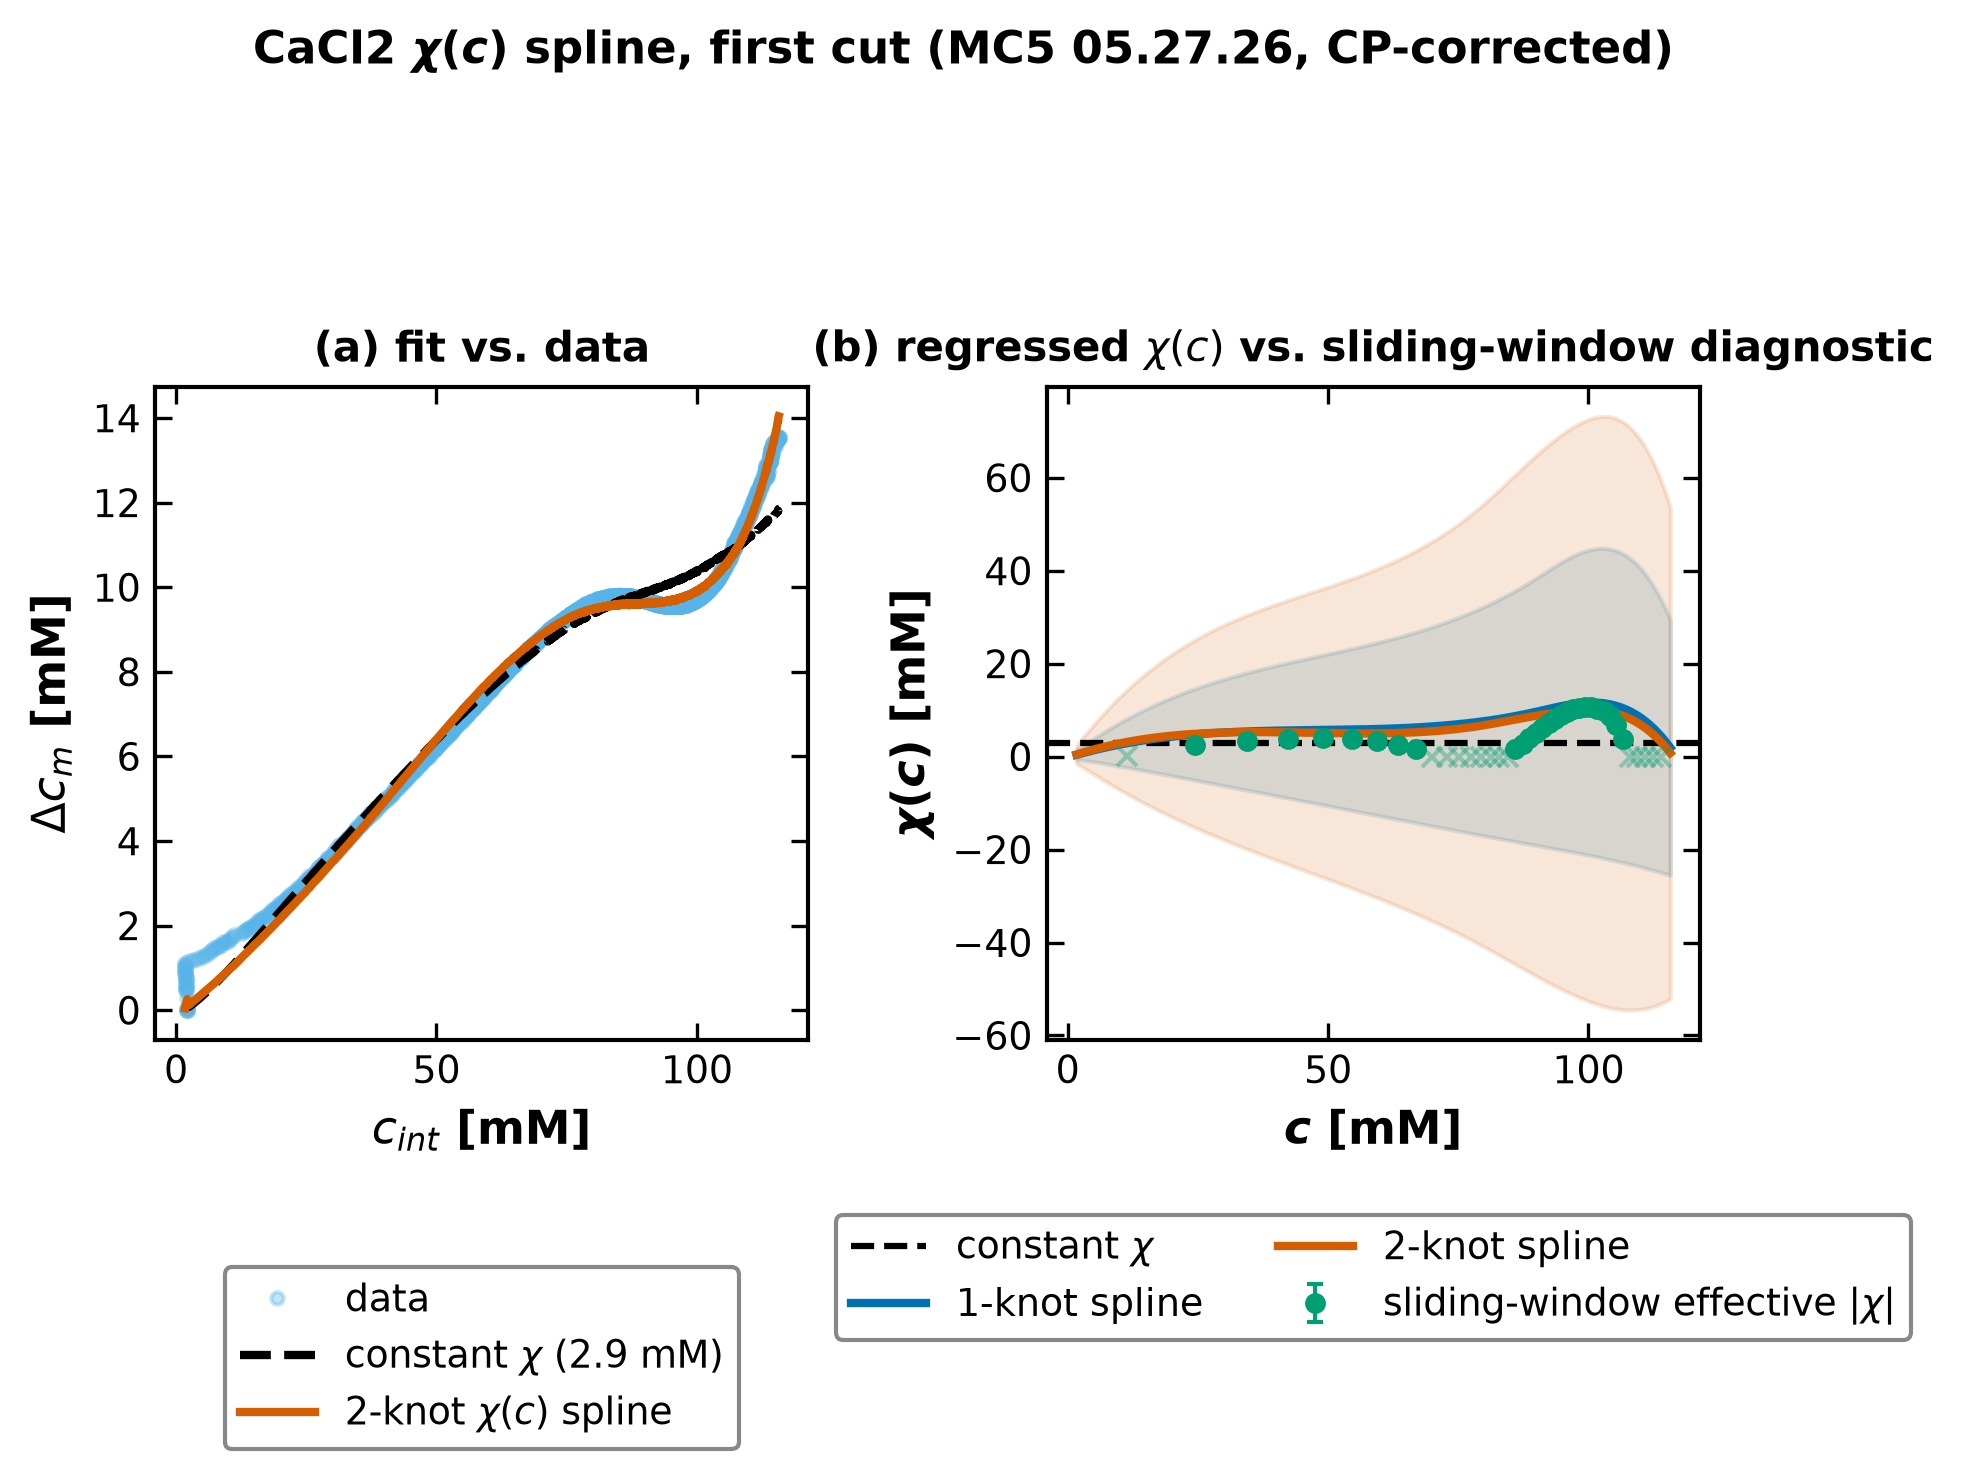
\includegraphics[width=\linewidth]{figures/cacl2_chispline_firstcut.png}
\caption{\ce{CaCl2} $\chi(c)$ spline first cut. \textbf{(a)} The constant-$\chi$
model (dashed) misses the data's smooth wave, which the spline follows.
\textbf{(b)} The regressed $\chi(c)$ (with $\pm1.96$ pointwise SE bands) against
the model-free sliding-window effective-$|\chi|$ (green). The point estimate
tracks the diagnostic (correlation $0.83$, RMSE $\SI{3.5}{mM}$), but the bands
are enormous --- $\chi(c)$ is only weakly identified pointwise, especially at
high $c$ where the co-ion is insensitive to charge (the bands are a linearized
Gauss--Newton approximation and ignore the $\chi\ge0$ bound, hence stray
negative).}
\label{fig:chispline}
\end{figure}

\paragraph{What this does and does not show.} The constant-charge model is
\textbf{clearly inadequate} for \ce{CaCl2}: an eight-fold $\SSE$ reduction, an
overwhelming $F$-test, and $100\%$-robust convergence say the data genuinely
demand concentration-dependent structure, and the regressed $\chi(\cint)$ tracks
the independent windowed diagnostic. \textbf{But the $\chi(c)$ shape cannot yet
be read as the adsorption isotherm}, for two reasons. First, $\chi(c)$ is poorly
identified \emph{as a function} --- the pointwise bands span tens of mM
(Fig.~\ref{fig:chispline}b), the fit is far better constrained than the
underlying $\chi(c)$. Second, and more important, a \textbf{null check on
\ce{NaCl}} --- the well-identified $1{:}1$ case with \emph{no} expected
adsorption drift --- fails: the same $1$-knot machinery, refitting $\dstar$
jointly, still improves the \ce{NaCl} fit significantly ($\SSE\ 52.4\to19.6$,
$F=286$, $\Delta$AIC $=-671$) with a decidedly non-flat $\hat\chi(c)$
(control-point spread $62\%$ of the mean). The likely mechanism is a
\textbf{time--concentration confound within a single run}: under
concentrating-lag diafiltration the feed concentration rises monotonically with
time, so a smooth function of $c$ is nearly interchangeable with a smooth
function of \emph{time}. An unpenalized $\chi(c)$ can therefore absorb any
slowly-varying temporal structure in the residuals --- in particular \ce{NaCl}'s
strong AR(1) autocorrelation ($\hat\phi\approx0.74$, \S\ref{sec:naclAR1}) ---
whether or not it reflects adsorption chemistry, and the i.i.d.\ $F$-test/AIC
used here do not know about that autocorrelation (the same anti-conservative
trap \S\ref{sec:naclAR1} flagged for the constant-$\chi$ regions). The same
flexibility likewise absorbs the calibration-source and transformed-vs-raw
mean-model questions (\S\ref{sec:condmodels}, \S\ref{sec:altform}). So the
\ce{CaCl2} improvement is real --- it robustly beats constant-$\chi$ and matches
an independent local estimator --- but this first cut \textbf{cannot yet rule
out that the drift is partly or wholly a time-correlated-noise artifact}, the
``clean mean model first'' risk this extension carries. It is suggestive, not
yet a green light for the full treatment.

\paragraph{AR(1)-whitened follow-up (outcome).} The cheap, decisive test proposed
above has now been run (\texttt{analysis/chi\_spline/chispline\_ar1\_whitened.py}):
re-estimate $\hat\phi$ from the constant-$\chi$ model's time-ordered residuals
(Cochrane--Orcutt, \S\ref{sec:naclAR1}'s Method A convention), whiten \emph{both}
the constant and $1$-knot-spline residual functions with that \emph{same} common
$\hat\phi$ (a fair, one-noise-model comparison), and redo the nested $F$-test on
the whitened SSE with the actual $n-p$ df.
\begin{table}[H]
\centering\small
\begin{tabular}{llccccc}
\toprule
Dataset & Regime & $\hat\phi$ & $F$ & $p$ & $\Delta$AIC & $\chi(c)$ spread \\
\midrule
\ce{NaCl}  & i.i.d.    & --     & $286.0$  & $\approx0$ & $-671$  & --- \\
\ce{NaCl}  & whitened  & $0.747$ & $27.8$   & $\approx0$ & $-96$   & $53\%$ of $\chi_0$ (not flat) \\
\ce{CaCl2} & i.i.d.    & --     & $2851.5$ & $\approx0$ & $-3404$ & --- \\
\ce{CaCl2} & whitened  & $0.999$ & $57.6$   & $\approx0$ & $-208$  & $563\times\ \chi_0$ (degenerate) \\
\bottomrule
\end{tabular}
\caption{AR(1)-whitened constant-vs-$1$-knot-spline comparison, common $\hat\phi$
per dataset (from the constant model, Cochrane--Orcutt-converged), actual $n-p$
df. \ce{NaCl}: $n=692$, $\hat\phi_{\mathrm{OLS}}=0.743\to0.747$ CO-converged
(matches \S\ref{sec:naclAR1}'s $0.743$ for the same primary dataset almost
exactly, as expected --- same residual series). \ce{CaCl2}: $n=1645$,
$\hat\phi_{\mathrm{OLS}}=0.995\to0.999$ CO-converged --- a \textbf{new} number
(the autocorrelation analysis of \S\ref{sec:naclAR1} only characterized
\ce{NaCl}).}
\label{tab:chispline-whitened}
\end{table}

\textbf{Neither branch of the proposed decision rule cleanly holds.}
\ce{NaCl}'s spurious drift is substantially \emph{weakened} by whitening
($F:286\to28$, $\Delta$AIC $-671\to-96$) but does \textbf{not evaporate}
($p\approx0$ still, control-point spread still $53\%$ of $\chi_0$) --- AR(1)
alone does not fully explain the confound, consistent with \S\ref{sec:naclAR1}'s
own finding that AR(1) is a large first-order correction but \emph{not fully
sufficient} for this residual series ($16$ of $30$ ACF lags still exceed the
band after whitening). \ce{CaCl2}'s side of the test is worse than
inconclusive --- it is \textbf{numerically degenerate}: $\hat\phi$ is already
$0.995$ from the raw OLS residuals (\emph{before} any Cochrane--Orcutt
iteration), i.e.\ far closer to a unit root than \ce{NaCl}'s $0.743$, and the
whitened $\chi(c)$ blows up to $\sim\!500$--$1700$\,\si{mM} (vs.\ a $\SI{2.95}{mM}$
constant estimate) --- physically meaningless. The likely reason: \ce{CaCl2}'s
constant-$\chi$ model is not just noisy but \emph{wrongly shaped} (that is the
entire premise of this section), so its OLS residuals are dominated by the
smooth, large-amplitude systematic wave that the spline is built to capture,
not by stationary AR(1) noise --- fitting an AR(1) process to residuals from a
badly mis-specified mean model is close to circular, and whitening at the
resulting near-unit-root $\hat\phi$ over-differences the signal along with any
noise. That $\hat\phi$ contrast is itself weakly informative, though: \ce{CaCl2}'s
constant-$\chi$ residuals are far more autocorrelated than \ce{NaCl}'s
($\hat\phi_{\mathrm{OLS}}=0.995$ vs.\ $0.743$) --- dominated by systematic
structure rather than stationary noise, consistent with (but not proof of)
genuine concentration-dependence, since a time-smooth calibration or temperature
artifact would leave the same signature. \textbf{Verdict: the confound is not
resolved by simple AR(1) whitening.}
For \ce{NaCl} it survives (weakened, not gone); for \ce{CaCl2} the test cannot
even be run cleanly, because the very mis-specification under investigation
contaminates the noise-model estimate needed to correct for it. This rules out
the ``AR(1) alone fixes it'' branch and points --- as anticipated --- toward
\textbf{pooling across differently-paced \ce{CaCl2} runs} (time and
concentration decorrelate \emph{across} runs even though they are collinear
within one) as the next step, rather than a richer single-run noise model.

\begin{figure}[H]
\centering
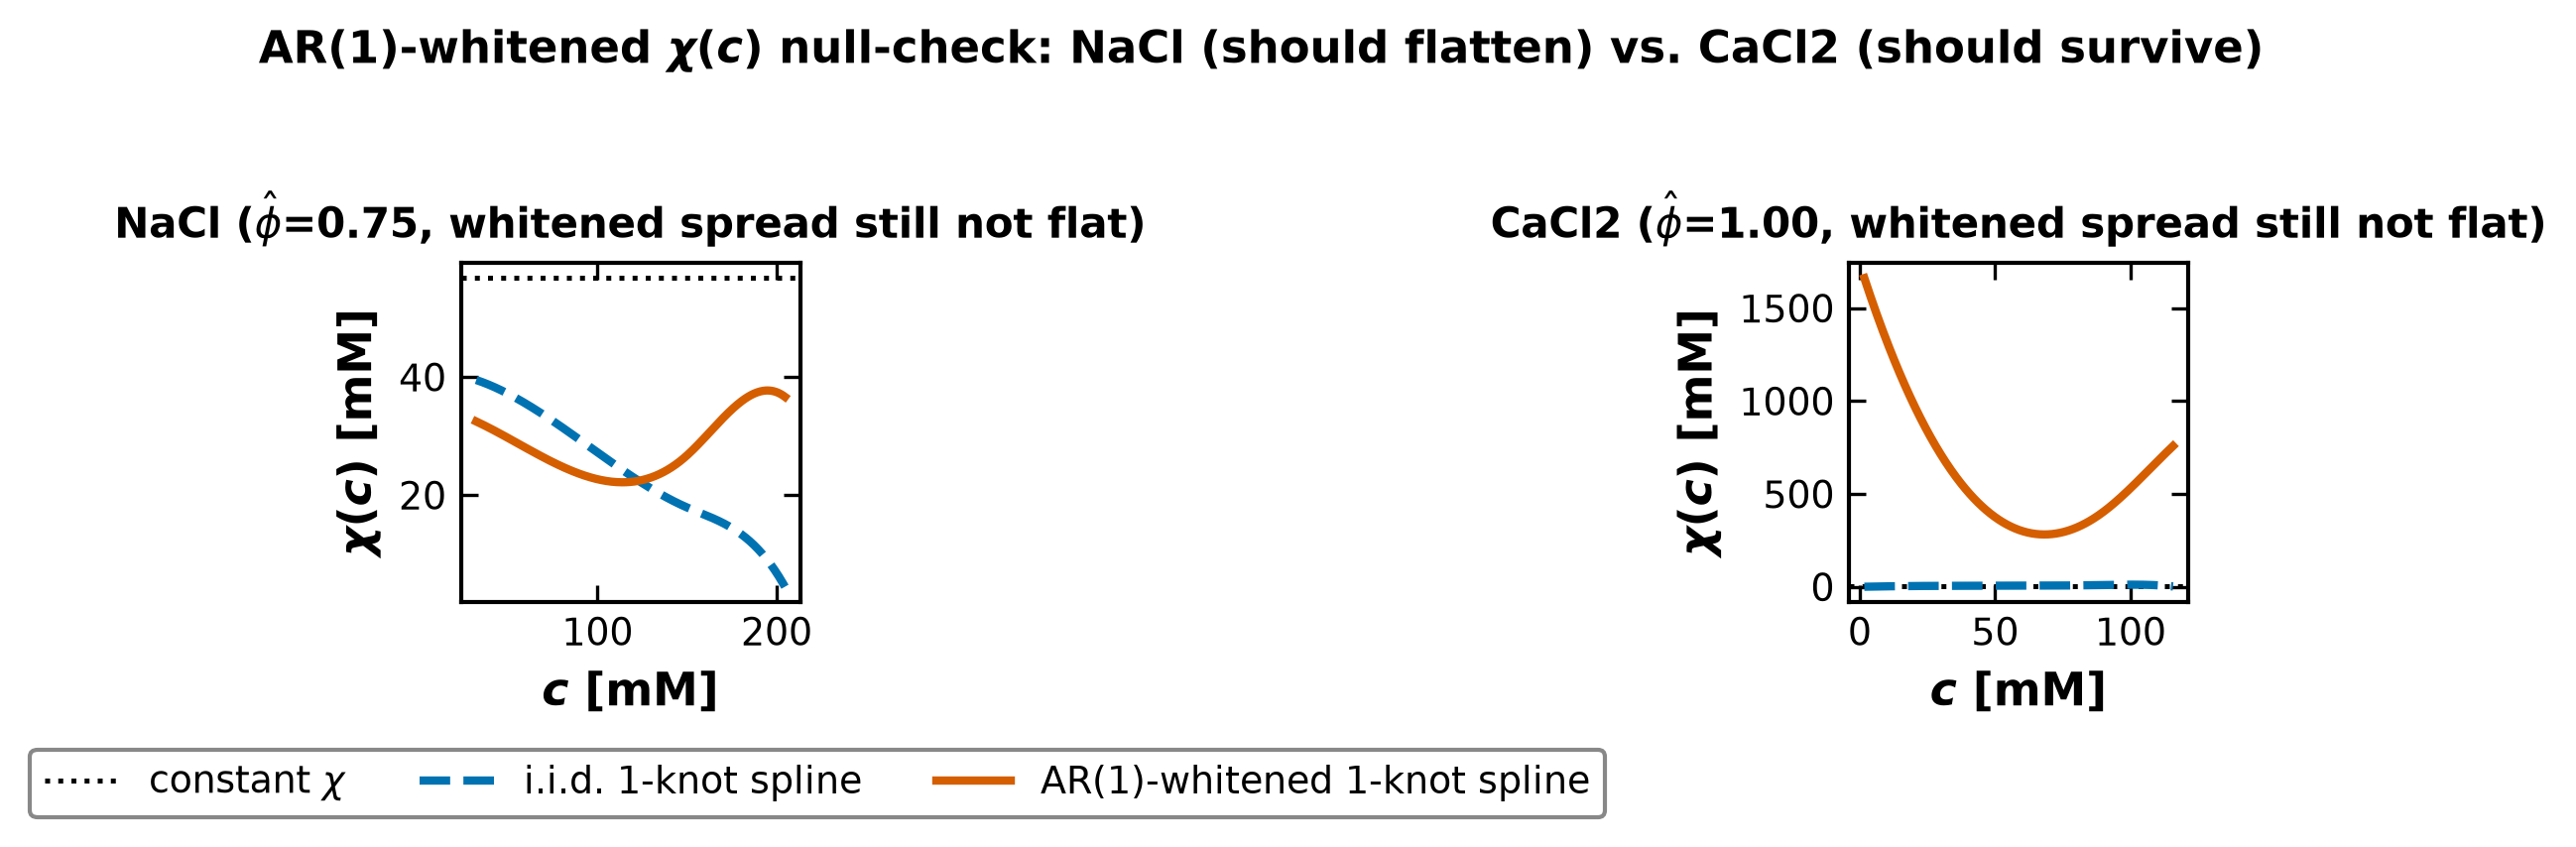
\includegraphics[width=\linewidth]{figures/cacl2_chispline_whitened.png}
\caption{AR(1)-whitened $\chi(c)$ (orange) vs.\ the i.i.d.\ fit (blue dashed)
and the constant estimate (black dotted), common $\hat\phi$ per dataset.
\textbf{\ce{NaCl}} (left): whitening changes the shape but does not flatten it
--- still not the flat line a true null result would show. \textbf{\ce{CaCl2}}
(right): the whitened curve is off by two to three orders of magnitude from the
constant estimate, the numerical signature of whitening at $\hat\phi\approx0.999$
described above --- not a usable estimate of $\chi(c)$, and not evidence for or
against real adsorption structure.}
\label{fig:chispline-whitened}
\end{figure}

\subsection{Recommended future work}\label{sec:chispline-future}
\begin{itemize}[itemsep=2pt]
  \item \textbf{Regularize.} Add a roughness penalty (P-spline) with a
        cross-validated smoothing parameter; the $1$-knot wiggle and the
        $2$-knot non-convergence both signal an under-constrained fit. This
        tames the pointwise bands and makes ``how many knots'' well-posed.
  \item \textbf{Disentangle before interpreting --- outcome of the cheap,
        decisive test.} The AR(1)-whitened re-run
        (\S\ref{sec:chispline-result}, ``AR(1)-whitened follow-up'') has now
        been done, and \textbf{neither branch of the original either/or held}:
        \ce{NaCl}'s spurious drift is weakened but does not evaporate under
        whitening, and \ce{CaCl2}'s own AR(1) diagnostic turns out to be
        numerically degenerate (its constant-$\chi$ residuals are dominated
        by the systematic mis-specification under test, not stationary
        noise, so $\hat\phi\to0.999$ and the whitened $\chi(c)$ blows up).
        A single-run AR(1) correction is therefore \textbf{not sufficient} to
        settle this either way. The confound must instead be broken by
        \textbf{pooling across differently-paced runs} (time and concentration
        decorrelate \emph{across} runs even though they are collinear within
        one), the eventual multi-dataset plan --- now the load-bearing next
        step, not an alternative to a richer single-run noise model. The
        calibration-source and errors-in-variables questions
        (\S\ref{sec:condmodels}, \S\ref{sec:altform}) should be settled in the
        same spirit before the shape is read as adsorption.
  \item \textbf{Generalize the numerics and UQ.} Move to the Pyomo/ParmEst
        nonlinear-constraint formulation (\S\ref{sec:lacl3impl}) for the
        quartic \ce{LaCl3} case and for proper profile/bootstrap intervals on
        $\chi(c)$; pool the three \ce{CaCl2} datasets for a shared $\chi(c)$.
  \item \textbf{Then, mechanism.} If a robust, penalized, multi-dataset
        $\chi(c)$ survives, fit a physical adsorption isotherm (e.g.\ Langmuir)
        to it for a few-parameter mechanistic interpretation --- the spline is
        the discovery tool, the isotherm the explanation.
\end{itemize}

% ############################################################
\section{Future extension: mechanistic partitioning (activity coefficients and dielectric exclusion)}\label{sec:partition}
% ############################################################
Throughout this report the non-electrostatic part of ion partitioning is carried
by a \emph{single lumped constant} --- $\dstar$ for the $1{:}1$ fit, $K$ for the
multivalent cases --- and the source Donnan theory \cite{multicompDonnanTheory}
takes the solutions to be \emph{ideal} ($\gamma_i=1$). This section lays out, as a
foreshadowed extension (no implementation here), how to replace that lump with
mechanistic partitioning physics, and why doing so bears directly on the central
open question of this report: is the multivalent misfit
(\S\ref{sec:cacl2diag}, \S\ref{sec:lacl3diag}, \S\ref{sec:copolymerdiag})
\emph{adsorption}, or missing \emph{non-ideality}?

\paragraph{A decomposed partitioning coefficient.} Equating the electrochemical
potential of each ion across the membrane interface,
$\mu_i=\mu_i^{\text{ref}}+RT\ln(\gamma_i c_i)+z_iF\psi+\mu_i^{\text{aff}}+\mu_i^{\text{exc}}$
with $\mu_i^{\mathrm s}=\mu_i^{\mathrm m}$ (Molly Dougher's derivation; the group
theory doc \cite{multicompDonnanTheory} combines the per-ion balances into the
single co-ion polynomial used above), gives a per-ion partitioning law
\begin{equation}
  \frac{\cm{i}}{\cs{i}}
  = \underbrace{\frac{\gamma_i^{\mathrm s}}{\gamma_i^{\mathrm m}}}_{\text{activity}}\,
    \underbrace{\phi_i^{\text{exc}}}_{\text{steric}}\,
    \underbrace{\phi_i^{\text{aff}}}_{\text{affinity}}\,
    \underbrace{\phi_i^{\text{diel}}}_{\text{dielectric}}\,
    \underbrace{\exp(-z_i\psi^{D})}_{\text{Donnan}}
  \;\eqqcolon\; \Phi_i\,\exp(-z_i\psi^{D}),
  \label{eq:partition}
\end{equation}
where $\psi^{D}=\psi^{\mathrm m}-\psi^{\mathrm s}$ is the Donnan potential (set by
membrane electroneutrality with $\chi$, as now) and $\Phi_i$ collects \emph{all}
non-electrostatic effects. \textbf{The present $\dstar$/$K$ is exactly a lumped,
concentration-independent $\Phi_i$ with $\gamma_i\equiv1$.} The extension is to
resolve $\Phi_i$ into physically-meaningful factors, most of which are
literature-parameterized rather than freely fit:
\begin{itemize}[itemsep=1pt]
  \item \textbf{Activity coefficients} $\gamma_i^{\mathrm s}/\gamma_i^{\mathrm m}$
        (TJ's work; the priority): relaxing $\gamma_i=1$ via an electrolyte model
        (extended Debye--H\"uckel / Davies / Pitzer), where $\ln\gamma_i\propto
        -z_i^2\sqrt{I}$ at leading order.
  \item \textbf{Dielectric exclusion} $\phi_i^{\text{diel}}=\exp(-\Delta W_i/k_BT)$
        with the Born solvation penalty $\Delta W_i=\frac{z_i^2 e^2}{8\pi\varepsilon_0 r_i}
        \big(\varepsilon_{\text{pore}}^{-1}-\varepsilon_{\text{bulk}}^{-1}\big)$ for
        a low-permittivity pore ($\varepsilon_{\text{pore}}<\varepsilon_{\text{bulk}}$);
        one parameter ($\varepsilon_{\text{pore}}$), an analytical form standard in
        the Donnan--steric-pore/dielectric-exclusion (DSPM--DE) membrane literature
        (Molly can supply the reference expression).
  \item \textbf{Steric exclusion} $\phi_i^{\text{exc}}=(1-\lambda_i)^2$,
        $\lambda_i=r_i/r_{\text{pore}}$ (known ion radii, one pore radius); and
        \textbf{affinity} $\phi_i^{\text{aff}}$ --- the specific ion--membrane
        interaction, which is where a \emph{genuine} adsorption term would live.
\end{itemize}

\paragraph{Why this could reframe the ``adsorption'' reading.} Both the activity
and dielectric factors scale as $z_i^2$, so they are negligible for $1{:}1$
\ce{NaCl} but grow sharply for the $2{:}1$/$3{:}1$/$1{:}2$ salts --- reproducing
the observed valence trend (clean \ce{NaCl}; $|\chi|\to0$ and effective-$\chi$
drift for \ce{CaCl2}/\ce{LaCl3}; the mixed copolymer \ce{Na2SO4} result) \emph{with
no adsorption invoked}. A constant-$\dstar$, $\gamma=1$ fit has nowhere to put this
$z_i^2$-scaled non-ideality except by distorting $|\chi|$, which is a plausible
mechanism for the very signatures \S\ref{sec:valencetrend} attributes to
adsorption. Molly's assessment is that activity coefficients are the leading
candidate for the $1{:}2$/$1{:}3$ discrepancies; the concrete test is direct ---
re-fit \ce{CaCl2}/\ce{LaCl3} with $\gamma_i$ (and/or $\phi_i^{\text{diel}}$)
included and ask whether $|\chi|$ stops collapsing and flattens with
concentration, the mechanistic counterpart of the $\chi(c)$-spline check
(\S\ref{sec:chispline}).

\paragraph{Estimability and a path.} The catch is that the dielectric and activity
terms are both $\propto z_i^2$, so they are mutually confounded --- and confounded
with $\chi$ --- on any \emph{single-valence} dataset. What separates them is
\textbf{multi-valence data}, and this program now has NaCl ($1{:}1$), \ce{CaCl2}
($2{:}1$), \ce{LaCl3} ($3{:}1$), and \ce{Na2SO4} ($1{:}2$): a \emph{joint}
regression across salts (shared membrane $\chi$, $\varepsilon_{\text{pore}}$,
$r_{\text{pore}}$; salt-specific but literature-known ion radii and diffusivities;
$\gamma_i$ from a fixed electrolyte model) uses the differing $z_i^2$ scalings to
identify each mechanism separately, with only a handful of free membrane
parameters. This is also the natural on-ramp to the multicomponent goal.
\note{Foreshadowed extension for a future session (after the $\chi(c)$-spline
work). Needs two inputs from the group: Molly's detailed partitioning write-up
(including the analytical dielectric-exclusion expression) and the specific
electrolyte activity-coefficient model from TJ's work (Davies vs.\ Pitzer;
external-solution only, or membrane phase too).}

% ############################################################
\section{Analysis plan with Claude Code}\label{sec:claude}
% ############################################################
This document and the accompanying code were produced with Claude Code using a
deliberate two-model division of labor.

\paragraph{Orchestration (Opus).} A single ``coordinator'' session (Claude Opus)
built scientific context (reading the DATA1/DATA2/Soft-Sensor papers
\cite{ouimet2022data1,liu2025data2,lilonfe2025softsensors}, Laurianne's
scanned Donnan notes \cite{donnan11notes,donnan21notes,donnan31notes}, Bill's
MATLAB \cite{billmatlab}, and the group's Word-document derivations
\cite{siDocx,donnanThermoDoc,transportDoc,boeDoc,manuscriptOutline,processModelDraft,multicompDonnanTheory}
--- the last extracted to \LaTeX\ via \texttt{pandoc}), inventoried the shared Box
folder, and \emph{reconciled} the mathematics across these sources (sign
conventions, the $\delta$ vs.\ $\dstar$ notation, and the factor-of-2 issue). It
maintains this consolidated writeup, decides modeling conventions, and drafts
well-scoped task prompts (saved under \texttt{docs/prompts/}).

\paragraph{Implementation (Sonnet).} Separate ``worker'' sessions (Claude Sonnet)
executed the well-scoped tasks, growing well beyond the original Step-2/3 scope:
the scipy port and ParmEst cross-validation (multi-start diagnostics, nonlinear
confidence regions); the raw$\to$processed preprocessing pipeline
(\S\ref{sec:preproc}) and its validation against six previously raw-only NaCl
runs; the \ce{CaCl2} and \ce{LaCl3} analyses (cubic/quartic root-solves,
nonlinear-constraint ParmEst formulations, adsorption-hypothesis diagnostics);
a whole-report figure-compliance audit (font scale, bold math, boxed legends,
\S\ref{sec:questions}-adjacent presentation fixes); the AR(1) autocorrelation
correction and its follow-up double-counting fix (\S\ref{sec:naclAR1}); the
raw-measurement reformulation (\S\ref{sec:altform}); and this cross-document
consistency/synthesis pass. The PI runs these sessions and passes their output
back to the coordinator for review and integration --- keeping a human
checkpoint between steps.

\paragraph{Reproducibility.} All analysis runs in a documented conda environment
(\texttt{environment.yml}, \texttt{data3-regression}); code lives under
\texttt{analysis/step*/} with per-step \texttt{README.md} files; figures are
regenerated into \texttt{docs/reports/figures/}. Project status has also been
presented to both groups
\cite{data3presentation2026,iconPoster2026,phillipLabUpdate2026}.

\paragraph{Lessons learned (so far).}
\begin{itemize}[itemsep=2pt]
  \item Having the stronger model \emph{reconcile multi-source mathematics} before
        any coding caught real discrepancies (factor of 2, sign conventions) that
        would otherwise have propagated into the regression.
  \item Read-only ``inventory'' subagents efficiently mapped a large ($\sim$683
        file) shared drive and extracted equations from Word documents.
  \item Delegating implementation with a \emph{self-contained} prompt (context +
        data paths + exact deliverables + what to report) let the worker sessions
        run end-to-end and return paste-ready numbers.
  \item Cross-validating two independent implementations (scipy vs.\ ParmEst)
        surfaced subtle tool traps (e.g.\ ParmEst's \texttt{measurement\_error}
        covariance scaling) and gave confidence in the estimates.
  \item An Opus audit of the AR(1) work (\S\ref{sec:naclAR1}) caught a
        \textbf{real statistical error} before it reached collaborators: an
        earlier draft combined GLS/whitening with an $n_{\mathrm{eff}}$
        degrees-of-freedom correction, double-counting the same
        autocorrelation and inflating the reported profile CI to a
        spurious $\sim\!8\times$ (vs.\ the correct $\sim$2.7--2.9$\times$
        non-CP at the time, now $\sim$2.5--2.7$\times$ CP-corrected).
        Catching this required recognizing that two statistically valid
        corrections for the \emph{same} effect are alternatives, not
        complements --- a subtlety easy to miss when each piece is
        individually correct.
  \item Iterative report-refinement and figure-compliance rounds (stale
        table/figure fixes, font-scale/legend/bold-math audits across every
        figure) were as important as the initial analysis for producing a
        document a collaborator can actually read and trust --- worth
        budgeting for explicitly, not treating as an afterthought.
\end{itemize}

% ############################################################
\section{Appendix: Per-Dataset NaCl Detail}\label{sec:naclappendix}
% ############################################################
\note{\textbf{Not yet refreshed to the CP-corrected convention:} every number
in this appendix is still the \textbf{non-CP} value (predating the
CP-corrected regression re-run); \S\ref{sec:naclAllResults}'s
summary table and figures ARE CP-corrected (primary). Refreshing all nine
individual write-ups below is flagged as remaining work, not silently stale.}
Full preprocessing and fit/residual detail for every one of the nine NaCl runs
summarized in \S\ref{sec:naclAllResults}, in the same order as
Table~\ref{tab:nacldata}. This appendix is intended as a complete reference for
each individual run (favoring completeness over brevity, per this document's
purpose as an internal working record) --- \S\ref{sec:naclAllResults} is the
place to read for the cross-dataset synthesis. For the three originally-processed
runs, only the fit + residuals panels apply (no reconstruction was needed); for
the six reconstructed raw-only runs, the calibration fit, $\Jw(t)$, and
reconstructed $\cint(t),\cp(t)$ panels are also shown.

\subsection{MC2 (05.07.24)}\label{sec:app-mc2}
Arrived pre-processed (Src [A], Table~\ref{tab:nacldata}); $n=482$. Corrected
model: $|\chi|=18.46$ (95\% CI $18.06$--$18.87$)\,mM, $\dstar=0.2888$ (CI
$0.2857$--$0.2920$), $\SSE=4.47$, 100\% multi-start convergence. This is the
narrow-concentration-range run ($\cint\lesssim\SI{44}{mM}$) discussed in
\S\ref{sec:naclAllResults} as a likely case of weak curvature/identifiability
rather than a different membrane.
\begin{figure}[H]
\centering
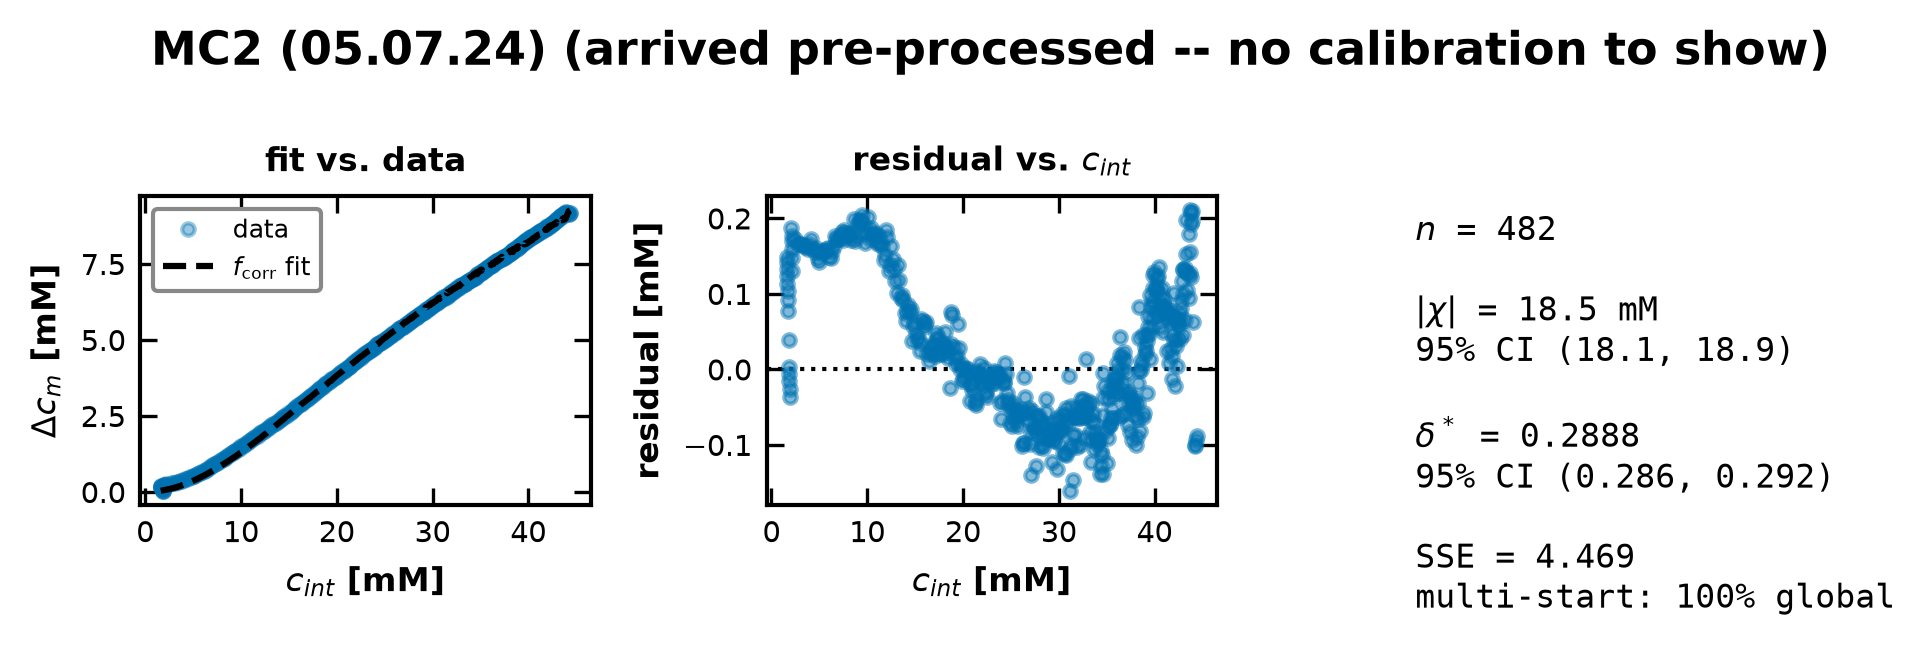
\includegraphics[width=\linewidth]{figures/nacl_appendix_mc2.png}
\caption{MC2 (05.07.24): fit vs.\ data, residual vs.\ $\cint$, and parameter
summary.}
\end{figure}

\subsection{MC5 (05.27.26)}\label{sec:app-mc5a}
Arrived pre-processed (Src [A]); $n=747$. Corrected model: $|\chi|=49.56$ (CI
$48.58$--$50.55$)\,mM, $\dstar=0.3251$ (CI $0.3232$--$0.3270$), $\SSE=130.07$,
100\% multi-start convergence. Matches its repeat (\S\ref{sec:app-mc5a2}) almost
exactly.
\begin{figure}[H]
\centering
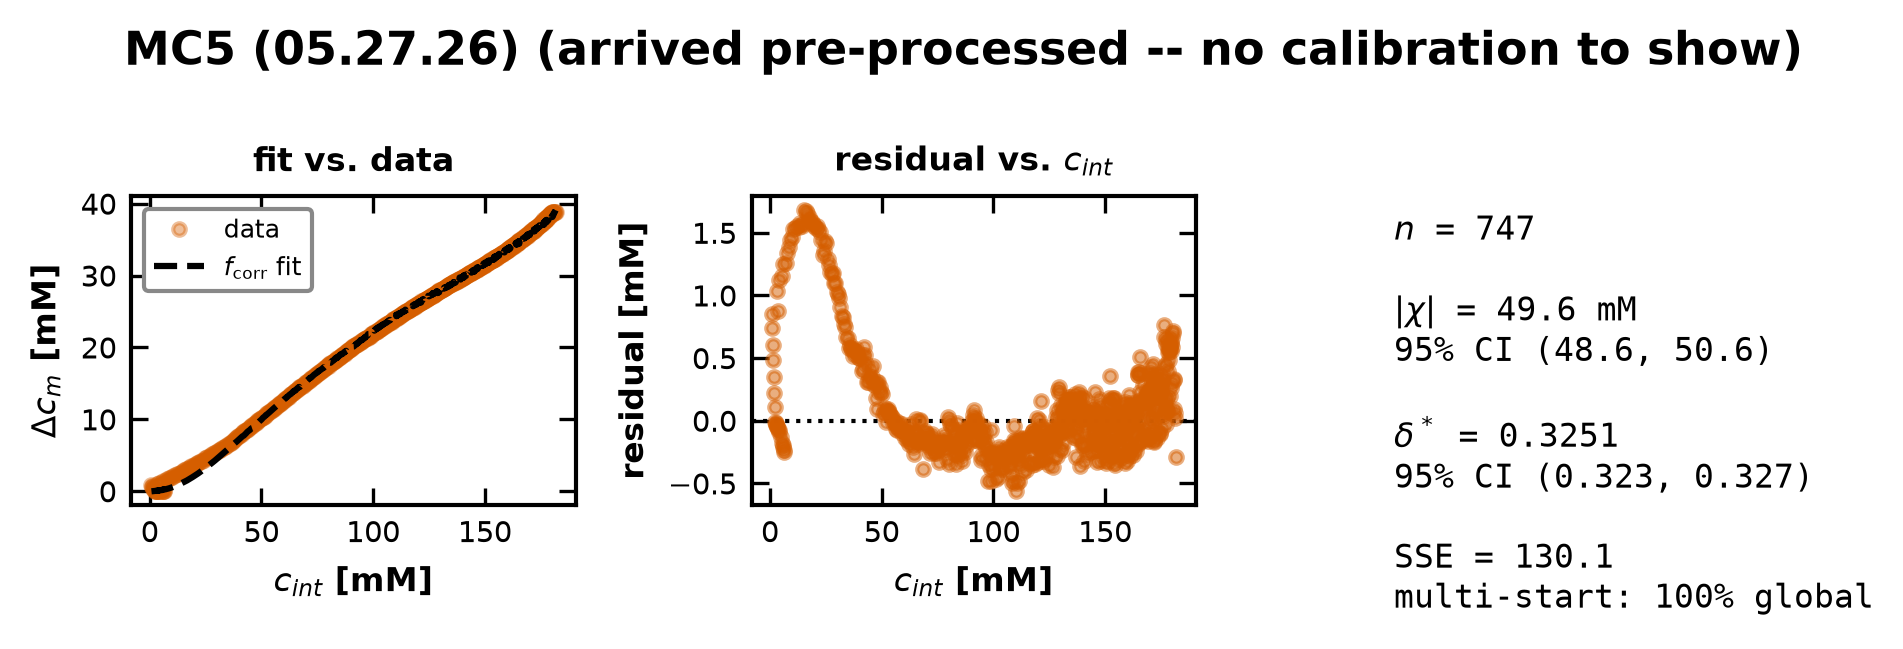
\includegraphics[width=\linewidth]{figures/nacl_appendix_mc5_0527.png}
\caption{MC5 (05.27.26): fit vs.\ data, residual vs.\ $\cint$, and parameter
summary.}
\end{figure}

\subsection{MC5 (05.27.26) (2)}\label{sec:app-mc5a2}
Arrived pre-processed (Src [A]); $n=747$. This is the \textbf{primary} NaCl
dataset analyzed in \S\ref{sec:reproMATLAB}--\ref{sec:naclUQ}. Corrected model:
$|\chi|=49.55$ (CI $48.58$--$50.54$)\,mM, $\dstar=0.3251$ (CI
$0.3232$--$0.3270$), $\SSE=129.62$, 100\% multi-start convergence.
\begin{figure}[H]
\centering
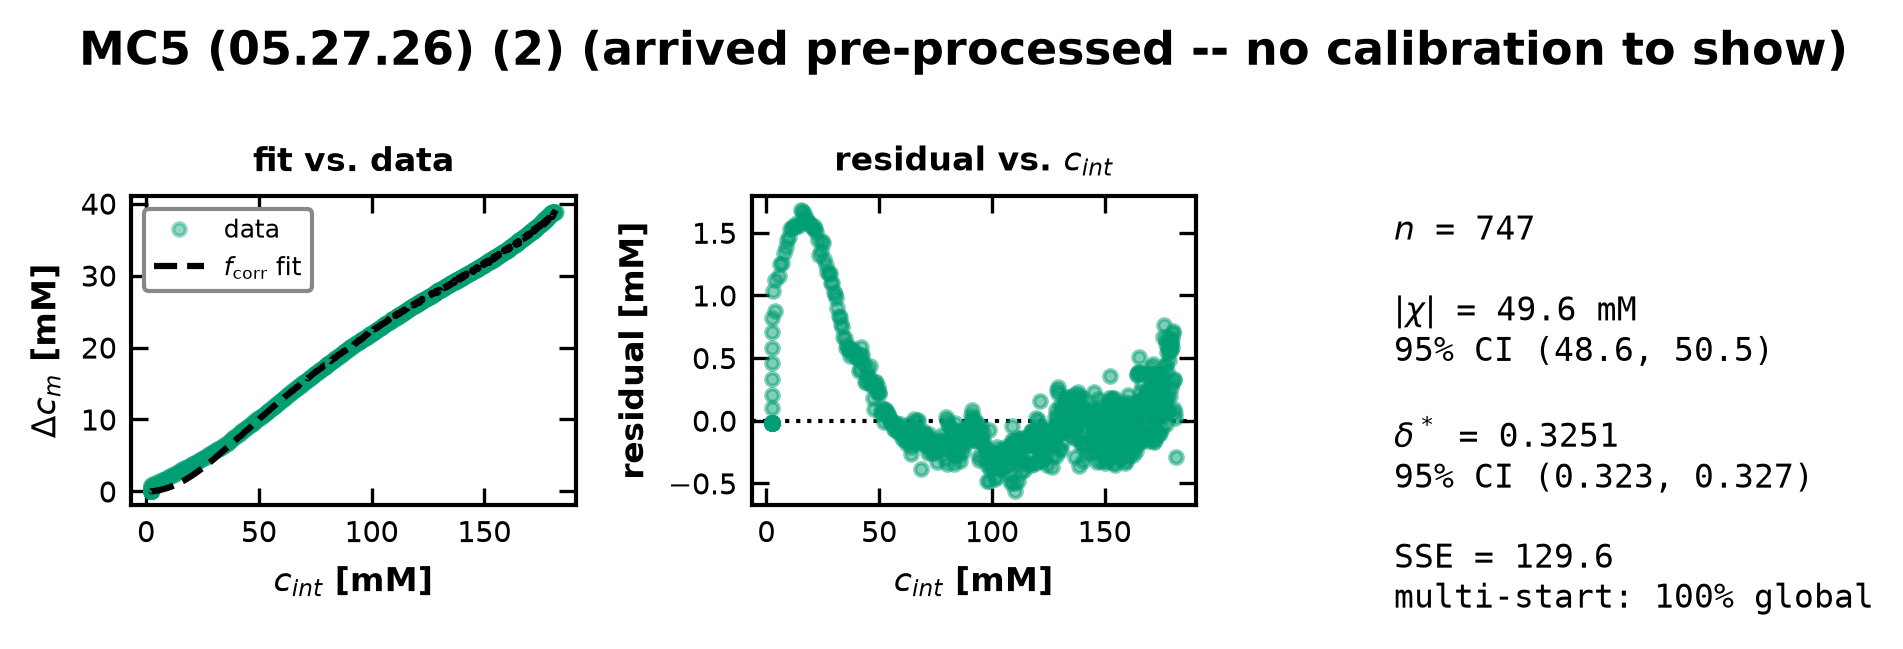
\includegraphics[width=\linewidth]{figures/nacl_appendix_mc5_0527_2.png}
\caption{MC5 (05.27.26) (2): fit vs.\ data, residual vs.\ $\cint$, and parameter
summary.}
\end{figure}

\subsection{MC3 (07.09.24)}\label{sec:app-mc3a}
Reconstructed from raw (\S\ref{sec:preproc}); per-experiment calibration
cond.\,$=145.0+98.0\,c$ ($R^2=0.9951$, $n=14$ vial points), consistent with the
other five reconstructed runs (\S\ref{sec:preproc} item~3). $n=391$ valid rows
after preprocessing. \textbf{This run does not converge}: the reconstructed
$\cint,\cp$ show a near-zero apparent rejection over most of the run (visible in
panel (c) below, where the two curves nearly overlap), which starves the
2-parameter Donnan model of curvature and lets \texttt{least\_squares} wander to
a nonphysical optimum ($|\chi|\to2.1\times10^6$\,mM). This is flagged (not
silently reported) as an ill-conditioned fit in Table~\ref{tab:naclall}.
\begin{figure}[H]
\centering
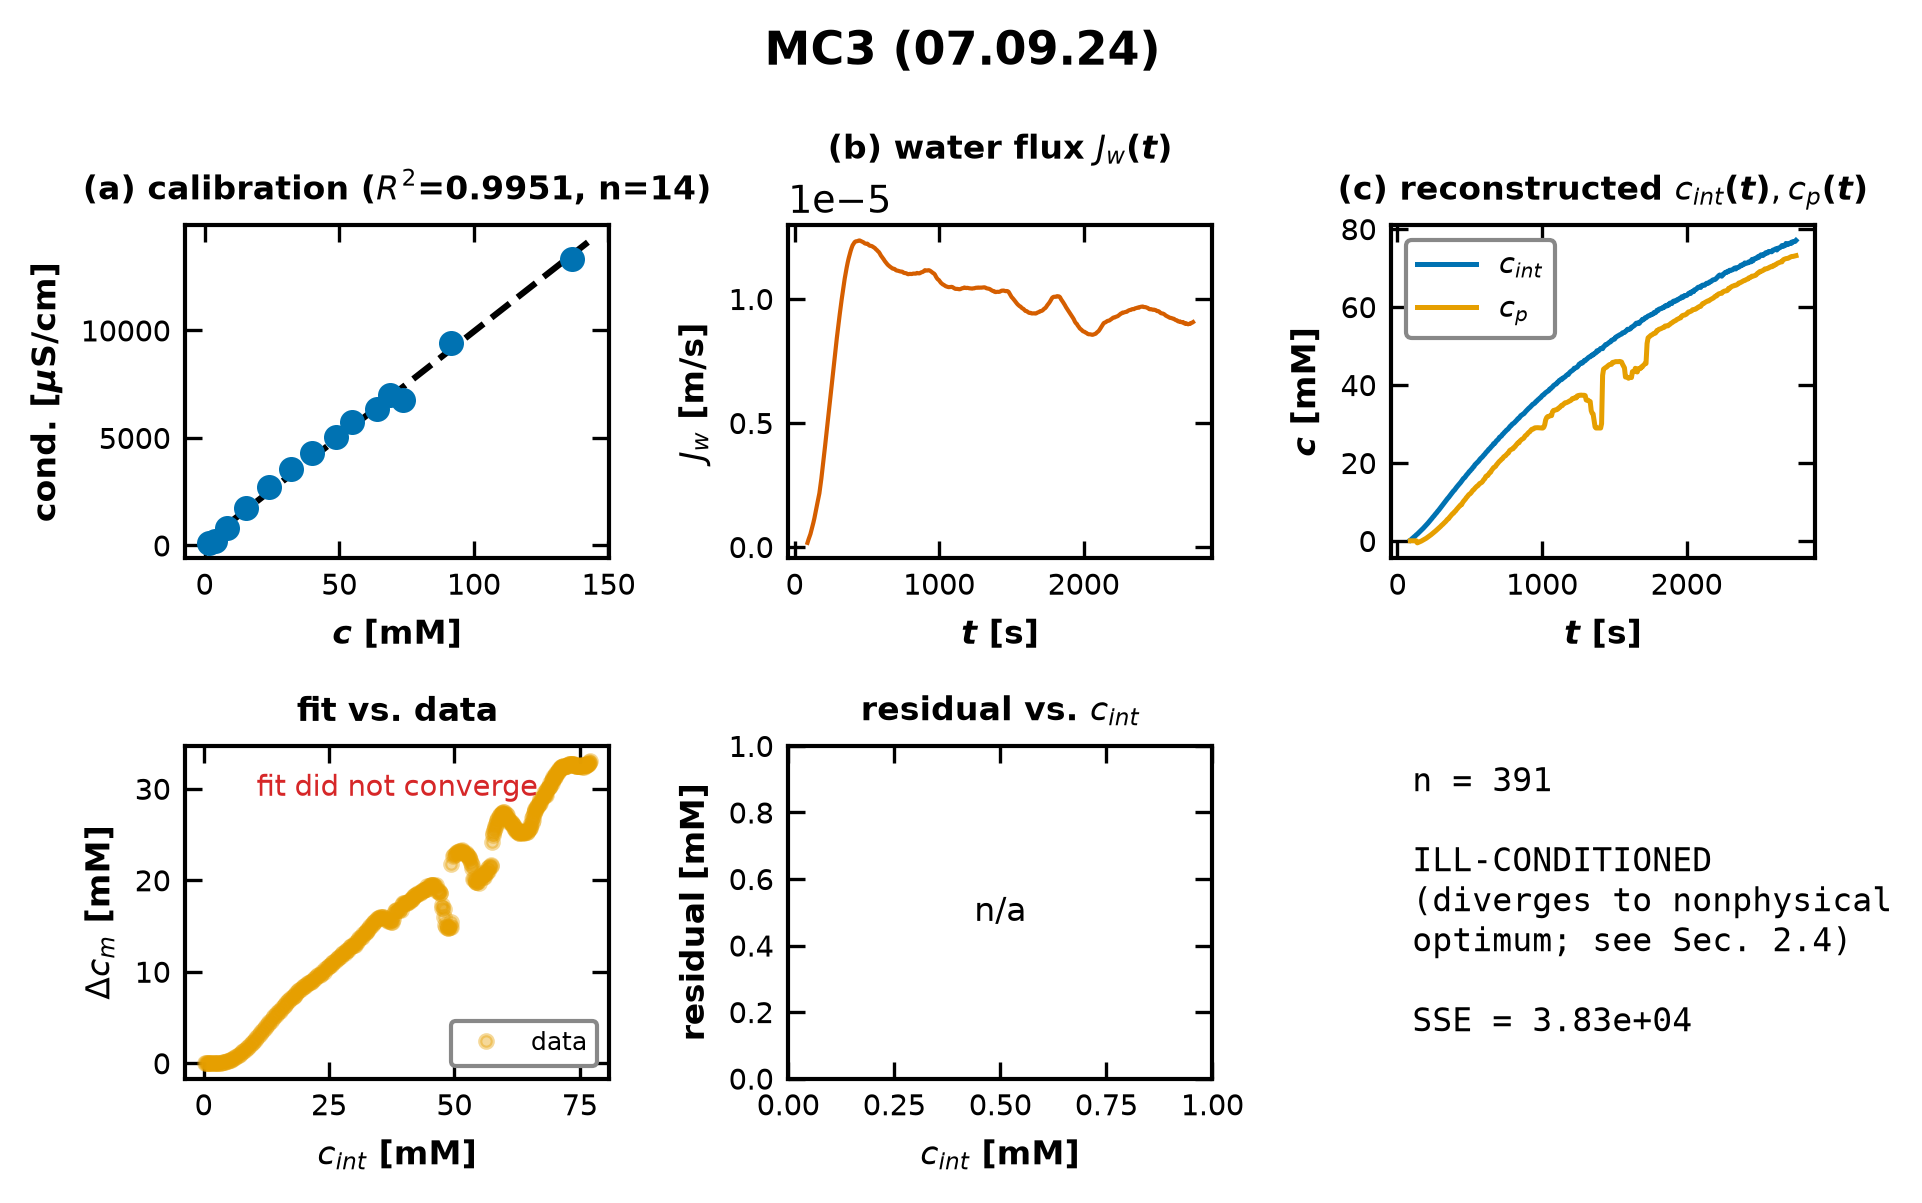
\includegraphics[width=\linewidth]{figures/nacl_appendix_mc3_0709.png}
\caption{MC3 (07.09.24): calibration, $\Jw(t)$, reconstructed $\cint(t),\cp(t)$,
fit vs.\ data (does not converge), residual vs.\ $\cint$ (n/a), and parameter
summary.}
\end{figure}

\subsection{MC3 (07.22.24, S)}\label{sec:app-mc3b}
Reconstructed from raw; per-experiment calibration cond.\,$=88.8+96.6\,c$
($R^2=0.9995$, $n=14$). $n=1312$ valid rows (a long sequential/reverse
``diluting'' run). Corrected model: $|\chi|=20.33$ (CI $12.44$--$31.91$)\,mM,
$\dstar=0.3000$ (CI $0.2484$--$0.3651$), $\SSE=101995$, 99\% multi-start
convergence. Poorly identified (95\% CI spans nearly $2\times$); the fit-vs-data
panel below shows the residual structure at high $\cint$ that later shows up as
extreme startup-trim sensitivity (\S\ref{sec:naclAllResults}).
\begin{figure}[H]
\centering
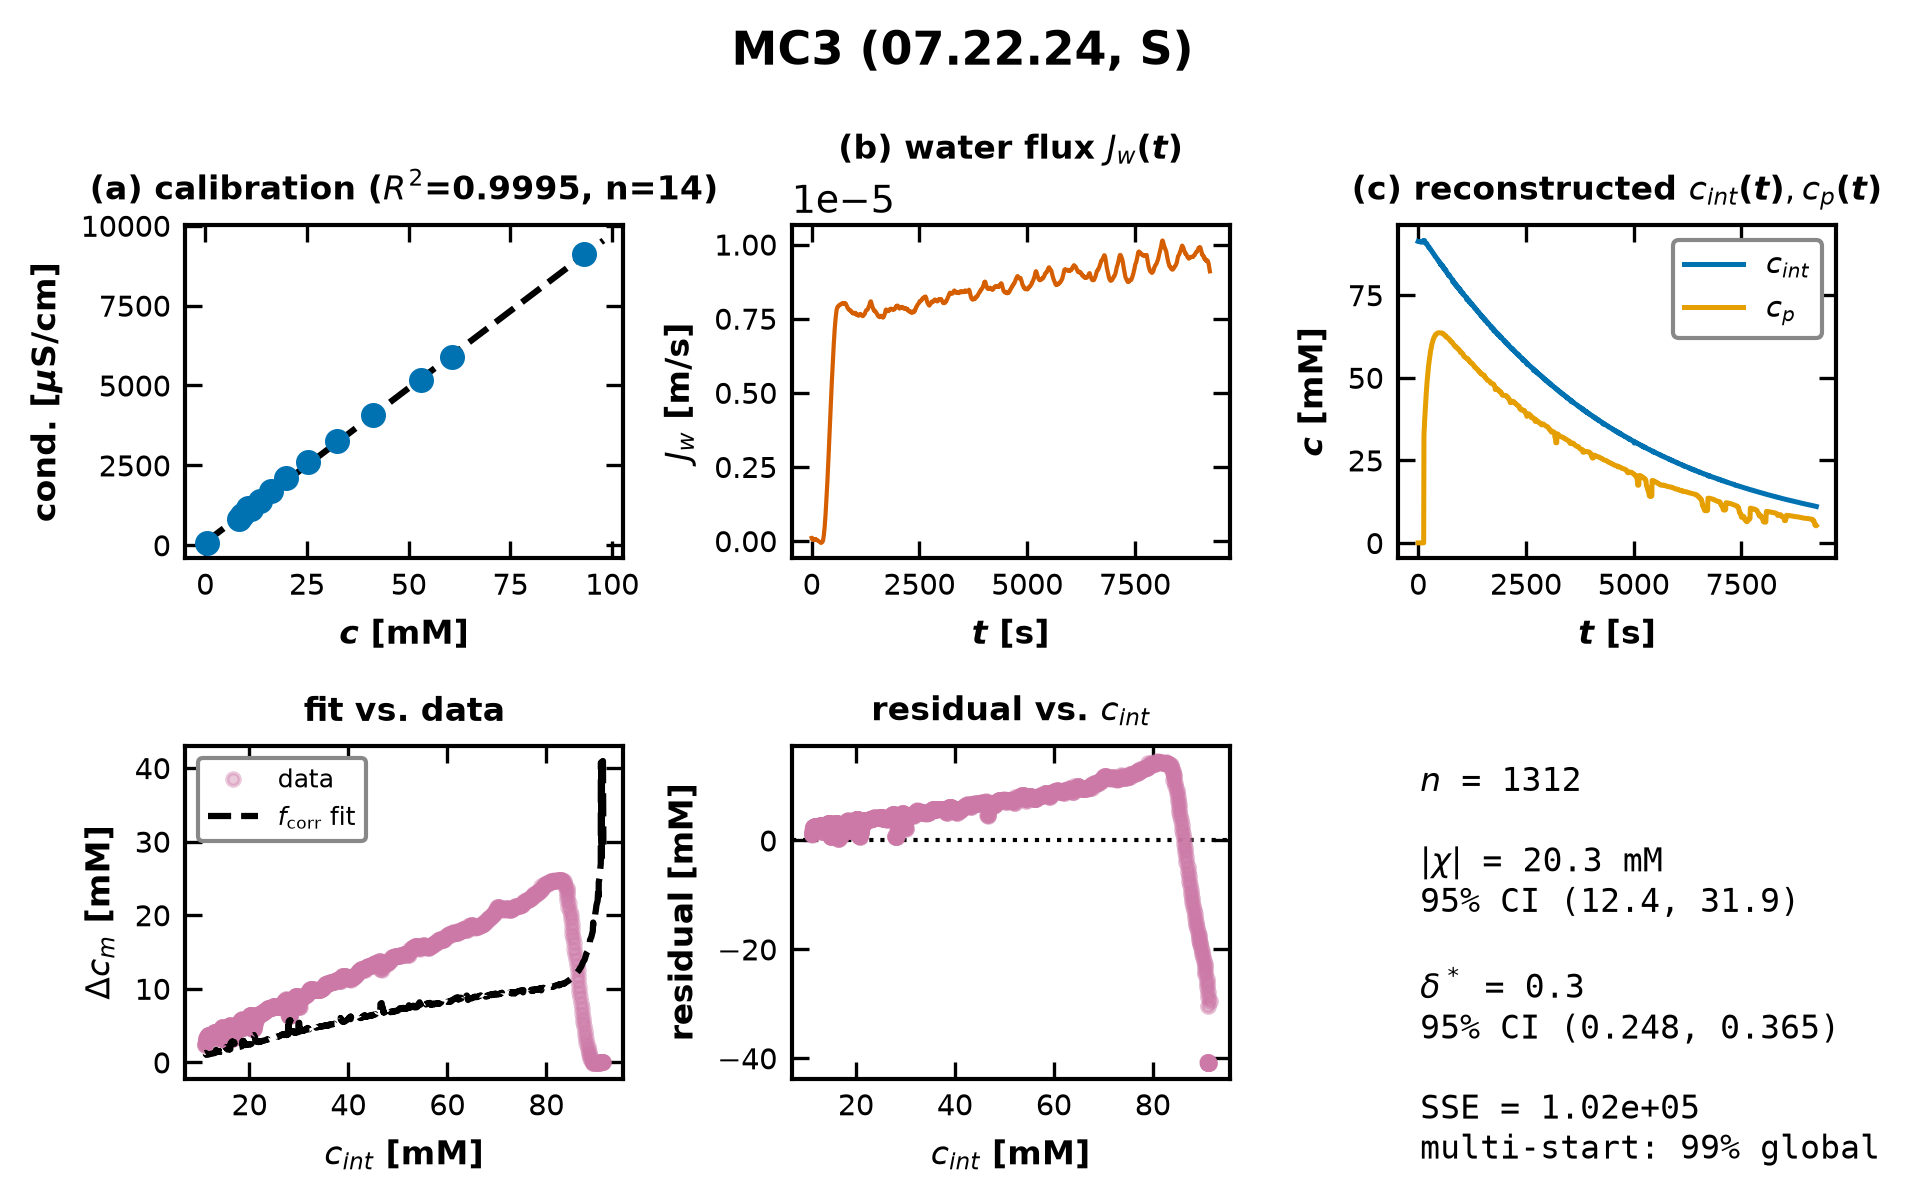
\includegraphics[width=\linewidth]{figures/nacl_appendix_mc3_0722s.png}
\caption{MC3 (07.22.24, S): calibration, $\Jw(t)$, reconstructed
$\cint(t),\cp(t)$, fit vs.\ data, residual vs.\ $\cint$, and parameter summary.}
\end{figure}

\subsection{MC4 (07.11.24, S)}\label{sec:app-mc4}
Reconstructed from raw; per-experiment calibration cond.\,$=17.4+95.4\,c$
($R^2=0.9971$, $n=13$ vial points -- one fewer than the other five runs, since
this run's ``Final Tube'' vial is missing a conductivity reading, but the fit
quality is unaffected, \S\ref{sec:preproc}). $n=317$ valid rows. Corrected
model: $|\chi|=106.63$ (CI $94.46$--$120.06$)\,mM, $\dstar=1.9313$ (CI
$1.8520$--$2.0214$), $\SSE=447.0$, 100\% multi-start convergence. Both
parameters are far outside the range of every other NaCl run (Fig.~\ref{fig:naclall}b) --
a real outlier among the reconstructed runs, not just a wide-CI one.
\begin{figure}[H]
\centering
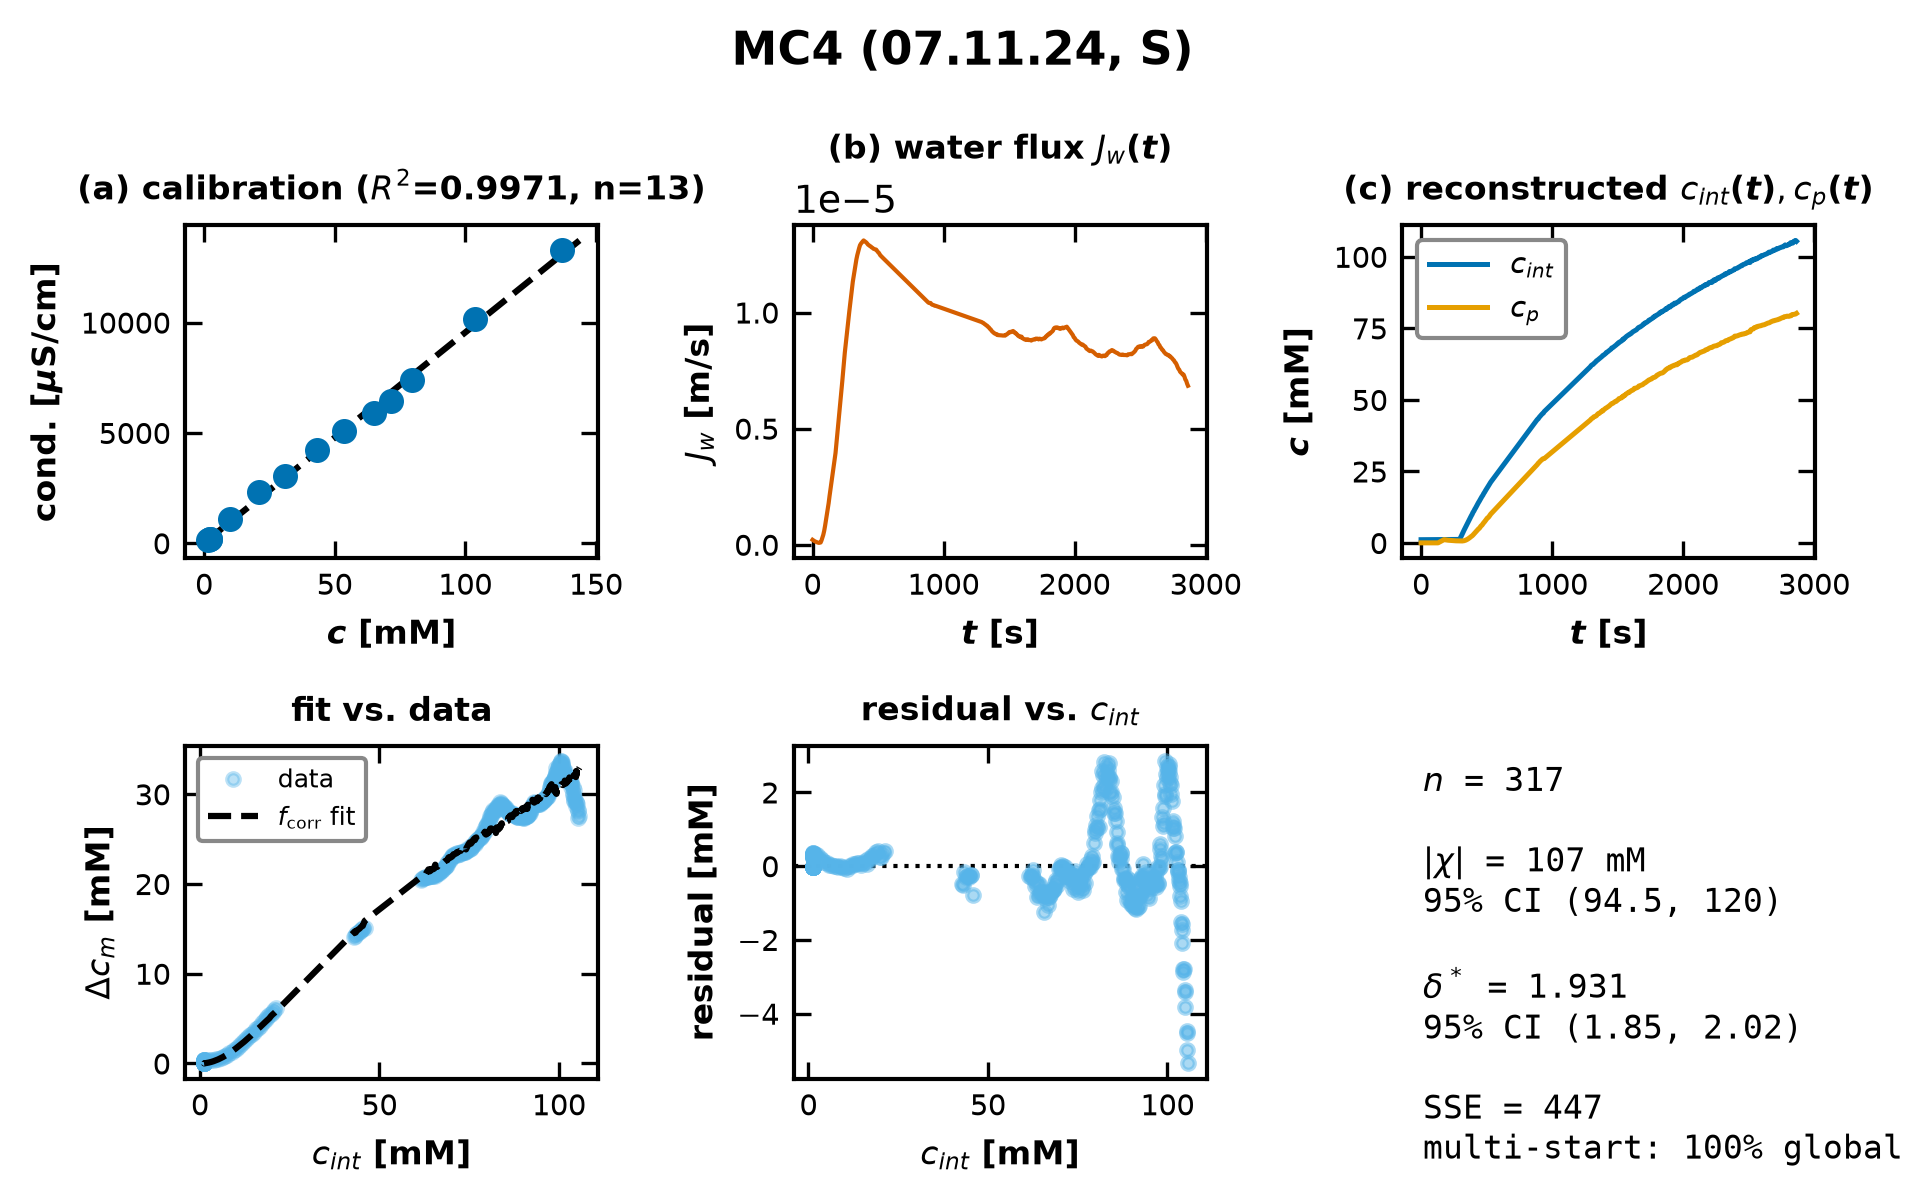
\includegraphics[width=\linewidth]{figures/nacl_appendix_mc4_0711s.png}
\caption{MC4 (07.11.24, S): calibration, $\Jw(t)$, reconstructed
$\cint(t),\cp(t)$, fit vs.\ data, residual vs.\ $\cint$, and parameter summary.}
\end{figure}

\subsection{MC5 (07.23.24)}\label{sec:app-mc5b}
Reconstructed from raw; per-experiment calibration cond.\,$=111.3+93.0\,c$
($R^2=0.9962$, $n=14$) -- this is the calibration shown as the representative
example in Fig.~\ref{fig:preprocvalid}a. $n=496$ valid rows. Corrected model:
$|\chi|=61.99$ (CI $60.53$--$63.49$)\,mM, $\dstar=0.7035$ (CI
$0.6966$--$0.7106$), $\SSE=52.9$, 100\% multi-start convergence. One of the
better-behaved reconstructed runs (95\% CI width $<5\%$, hence included in the
well-identified zoom of Fig.~\ref{fig:naclall}a) but still $\sim$25\% off MC5
(05.27.26)'s $|\chi|$ -- a reconstruction-pipeline discrepancy, not a
data-quality one for this specific run.
\begin{figure}[H]
\centering
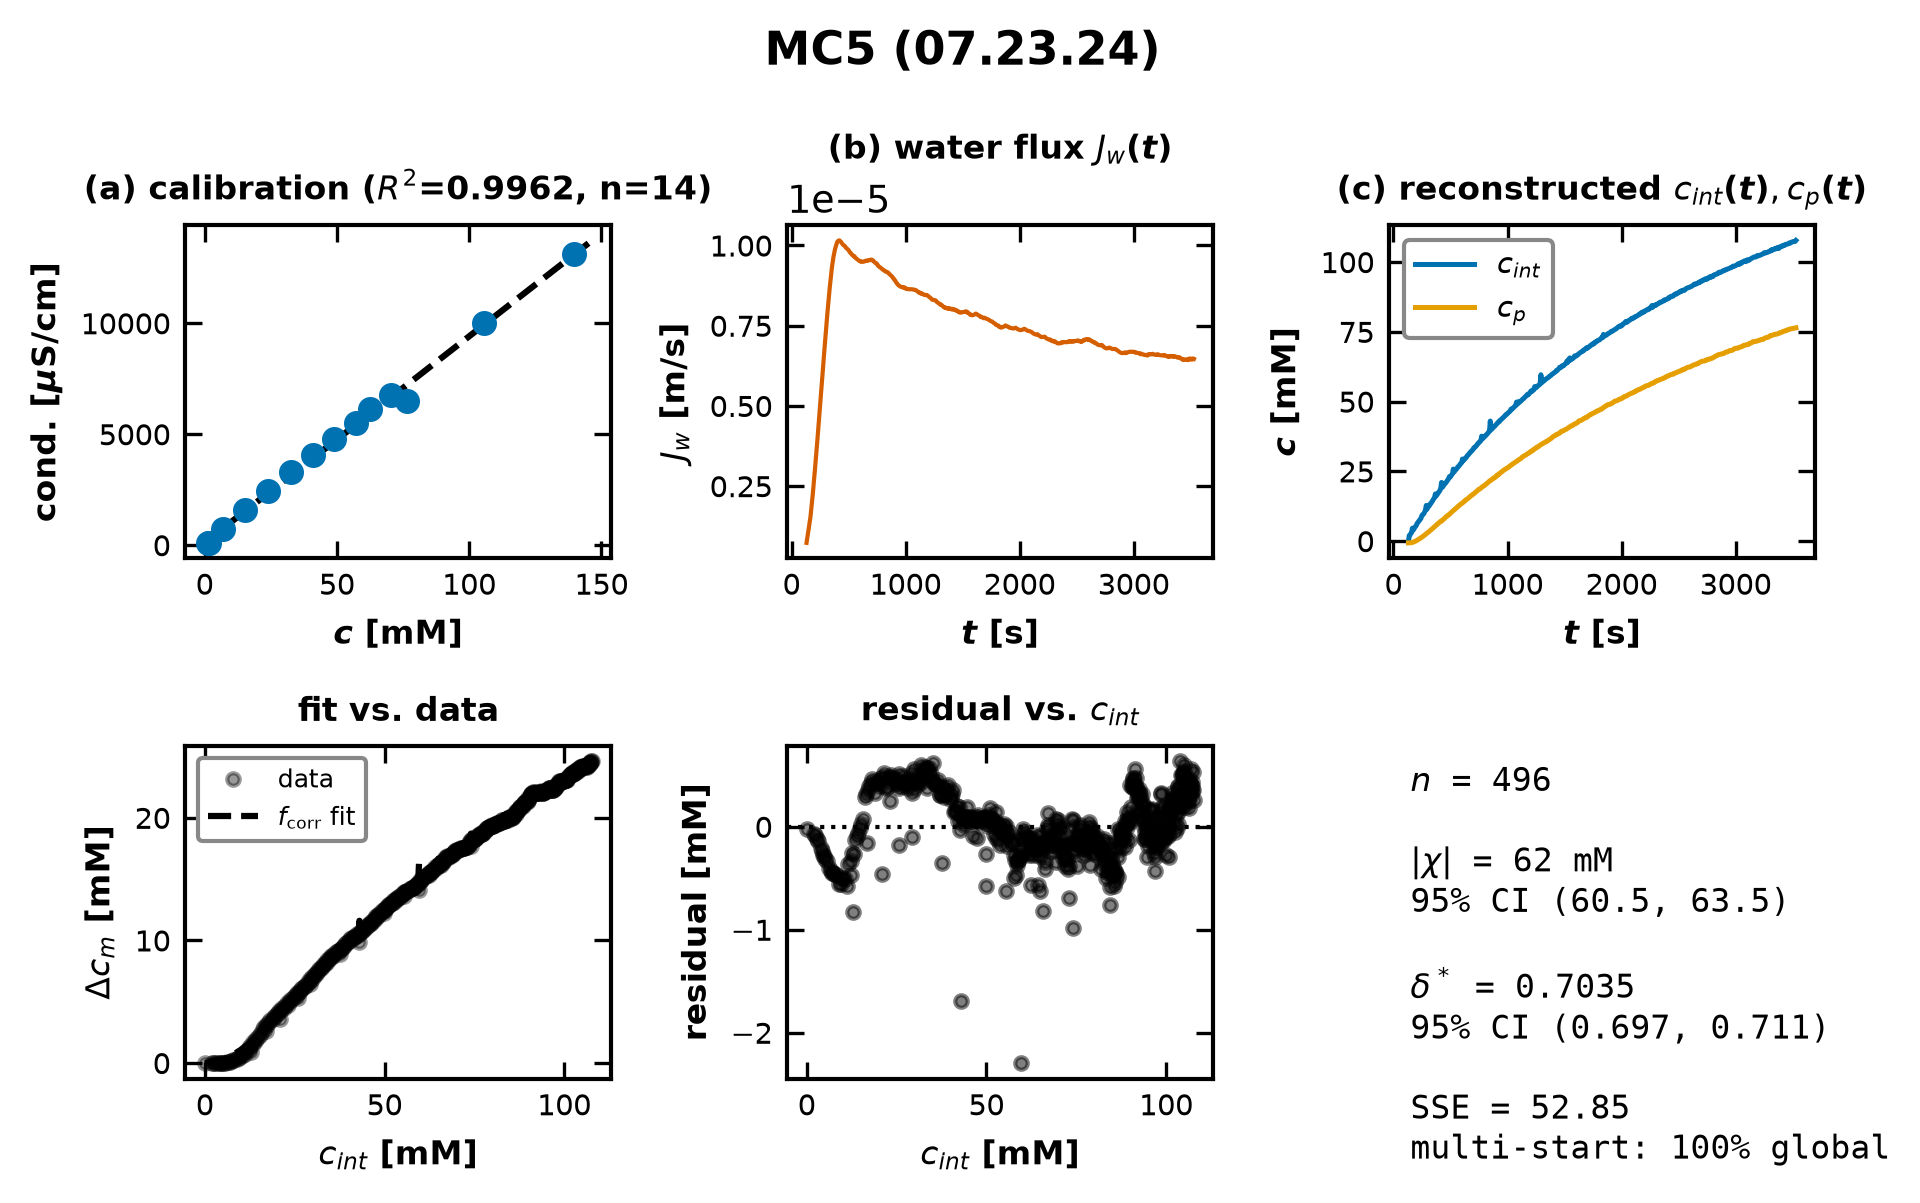
\includegraphics[width=\linewidth]{figures/nacl_appendix_mc5_0723.png}
\caption{MC5 (07.23.24): calibration, $\Jw(t)$, reconstructed
$\cint(t),\cp(t)$, fit vs.\ data, residual vs.\ $\cint$, and parameter summary.}
\end{figure}

\subsection{MC5 (07.23.24, S)}\label{sec:app-mc5c}
Reconstructed from raw; per-experiment calibration cond.\,$=177.0+93.2\,c$
($R^2=0.9965$, $n=14$). $n=500$ valid rows. Corrected model: $|\chi|=169.15$ (CI
$88.07$--$534.92$)\,mM, $\dstar=0.7147$ (CI $0.4415$--$1.9529$), $\SSE=11690$,
100\% multi-start convergence. \textbf{The worst-identified run in the whole
set}: the 95\% CI on $|\chi|$ spans a factor of $6\times$. The fit-vs-data panel
below shows why -- a pronounced high-$\cint$ divergence (the reverse/diluting
tail) that the 2-parameter model cannot track.
\begin{figure}[H]
\centering
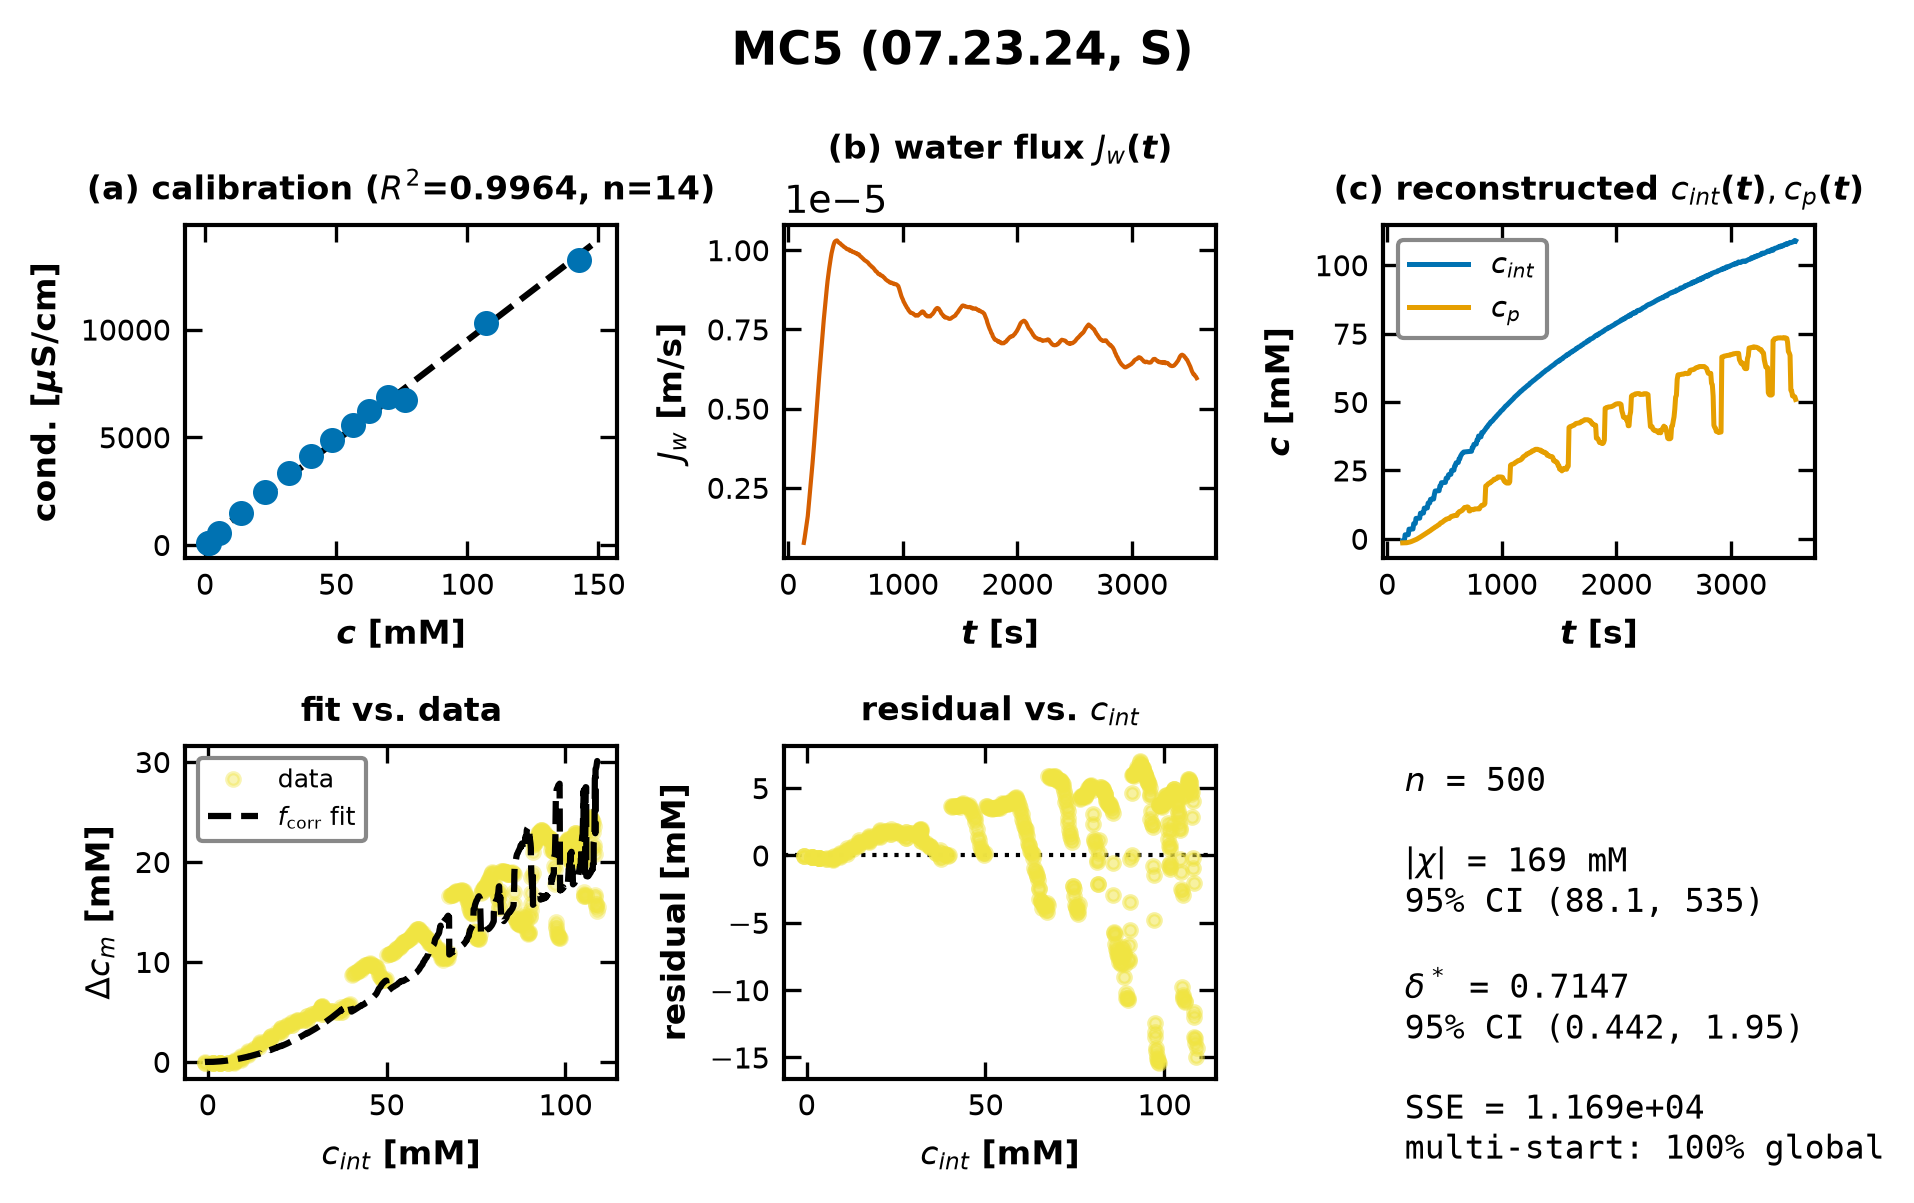
\includegraphics[width=\linewidth]{figures/nacl_appendix_mc5_0723s.png}
\caption{MC5 (07.23.24, S): calibration, $\Jw(t)$, reconstructed
$\cint(t),\cp(t)$, fit vs.\ data, residual vs.\ $\cint$, and parameter summary.}
\end{figure}

\subsection{MC5 (07.23.24, S2)}\label{sec:app-mc5d}
Reconstructed from raw; per-experiment calibration cond.\,$=136.7+98.4\,c$
($R^2=0.9991$, $n=14$). $n=1324$ valid rows (the longest run, another
sequential/reverse ``diluting'' protocol). Corrected model: $|\chi|=35.63$ (CI
$24.45$--$52.10$)\,mM, $\dstar=0.3434$ (CI $0.2801$--$0.4312$), $\SSE=68556$,
100\% multi-start convergence -- the only reconstructed run whose 95\% CI
overlaps MC5 (05.27.26)'s. Like MC5 (07.23.24, S) above, the fit-vs-data panel
shows a high-$\cint$ ``hook'' where the reverse/diluting protocol's data
deviates from the corrected model; this is the shared failure mode of both
\texttt{S}/\texttt{S2} runs (\S\ref{sec:naclAllResults}).
\begin{figure}[H]
\centering
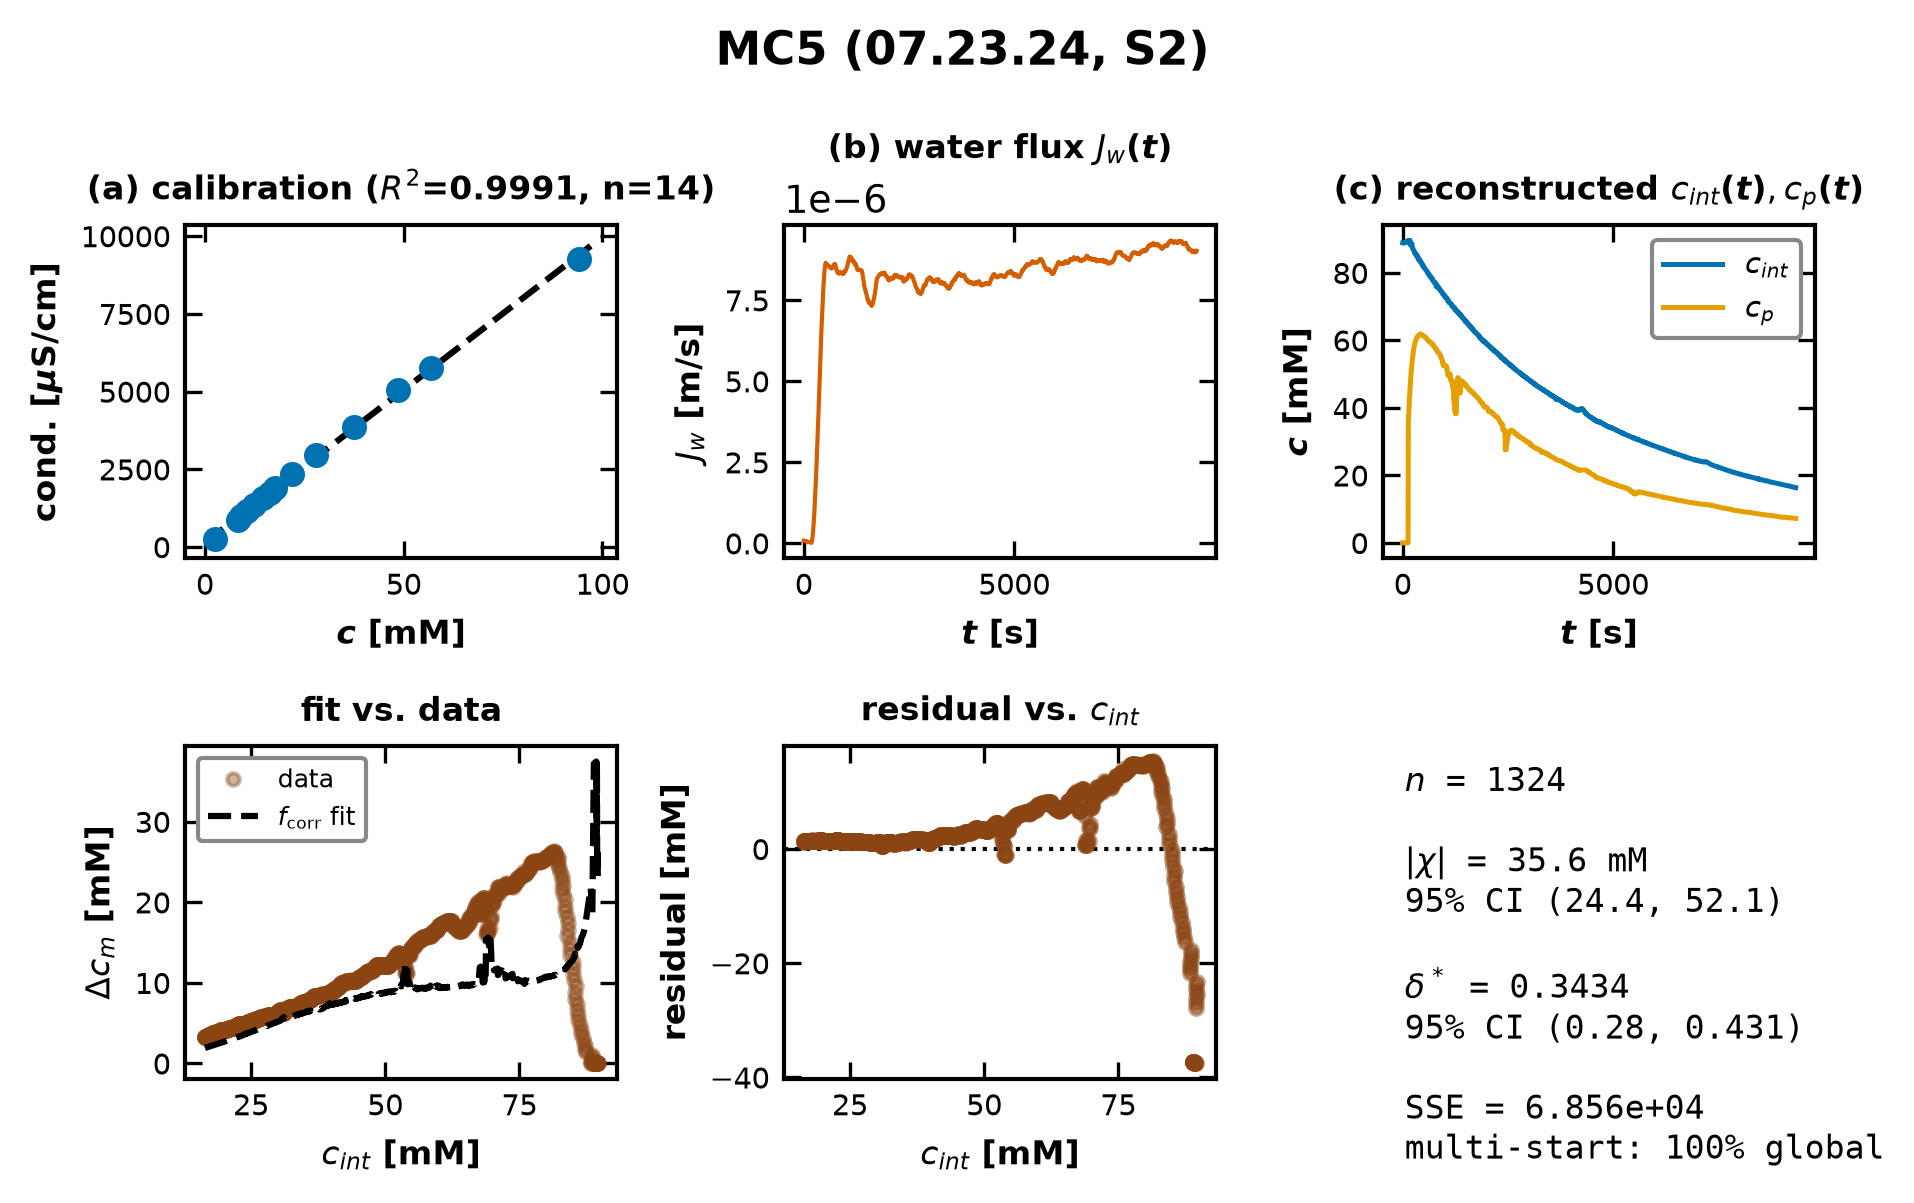
\includegraphics[width=\linewidth]{figures/nacl_appendix_mc5_0723s2.png}
\caption{MC5 (07.23.24, S2): calibration, $\Jw(t)$, reconstructed
$\cint(t),\cp(t)$, fit vs.\ data, residual vs.\ $\cint$, and parameter summary.}
\end{figure}

% ############################################################
\section{Appendix: Per-Dataset \ce{CaCl2} Detail}\label{sec:cacl2appendix}
% ############################################################
\note{\textbf{Not yet refreshed to the CP-corrected convention:} every number
in this appendix is still the \textbf{non-CP} value (predating the
CP-corrected regression re-run); \S\ref{sec:cacl2results}'s
summary table and figures ARE CP-corrected (primary). Refreshing all three
individual write-ups below is flagged as remaining work, not silently stale.}
Full fit/residual/drift detail for every one of the three processed \ce{CaCl2}
runs summarized in \S\ref{sec:cacl2results}, in the same order as
Table~\ref{tab:cacl2data}. As with \S\ref{sec:naclappendix}, this appendix is
a complete per-run reference (favoring completeness over brevity); read
\S\ref{sec:cacl2results}--\ref{sec:cacl2diag} for the cross-dataset synthesis.
Each figure shows (a) the corrected-model fit vs.\ data, (b) the residual vs.\
$\cint$ (with its sign-runs $z$-score), (c) the sliding-window effective
$|\chi|(\cint)$ diagnostic, and (d) the parameter/CI/fit-quality summary.

\subsection{MC3 (07.11.24, S)}\label{sec:app-cacl2-mc3}
$n=609$, $\cint\in[1.0,47]$\,mM (the narrowest-range \ce{CaCl2} run). Bounded
fit: $|\chi|\approx0$ (95\% CI $0$--$204.9$\,mM -- very poorly identified, the
narrow concentration range gives weak curvature), $K=0.02374$ (CI
$0.02318$--$0.02432$), $\SSE=388.3$, pseudo-$R^2=0.945$, 100\% multi-start
convergence. Residual sign-runs $z=-23.6$ (strongly non-random). Of its 14
sliding windows, only 5 are reliably identified (large-SE/boundary-pinned
windows excluded from the trend), rising from $\sim\!4$ to $\sim\!18$\,mM over
$\cint=35$--$47$\,mM -- consistent with sitting on the rising leg of the same
shape the wider-range MC5 runs show in full (\S\ref{sec:cacl2diag}).
\begin{figure}[H]
\centering
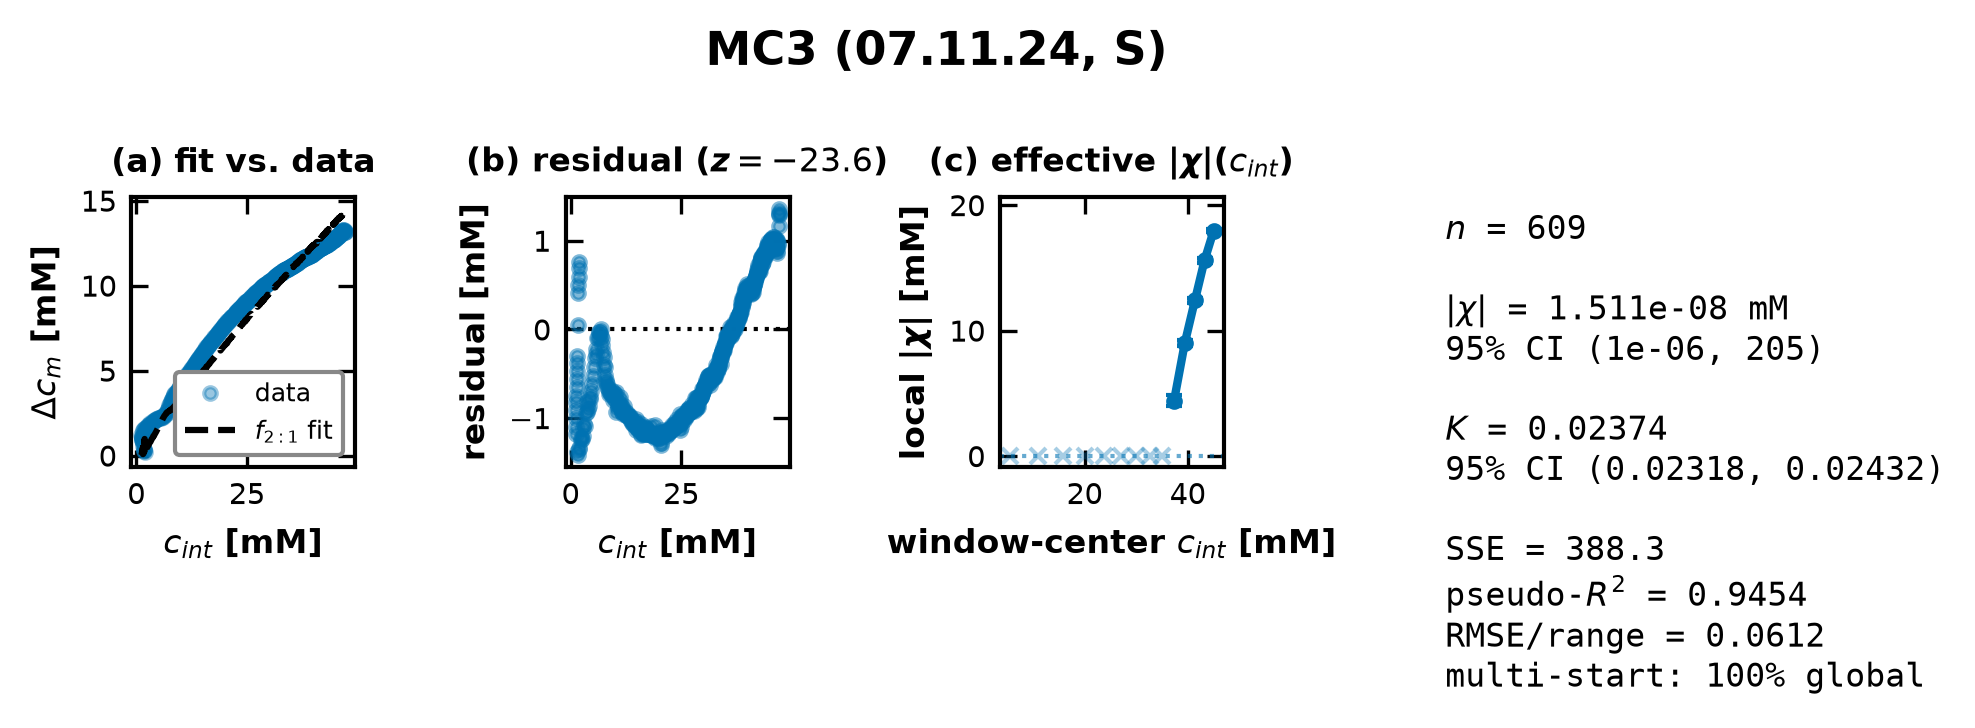
\includegraphics[width=\linewidth]{figures/cacl2_appendix_mc3_0711s.png}
\caption{MC3 (07.11.24, S): fit vs.\ data, residual vs.\ $\cint$, effective
$|\chi|(\cint)$, and parameter summary.}
\end{figure}

\subsection{MC5 (05.27.26)}\label{sec:app-cacl2-mc5a}
$n=1645$, $\cint\in[1.6,108]$\,mM. Bounded fit: $|\chi|=0.0176$ (95\% CI
$0$--$0.369$\,mM), $K=0.00080$ (CI $0.00079$--$0.00081$), $\SSE=643.2$,
pseudo-$R^2=0.937$, 96\% multi-start convergence. Residual sign-runs
$z=-39.8$. The effective-$|\chi|$ window fit is well identified (17 of 40
windows reliable) and shows the inverted-U rise-to-$\sim\!13$\,mM-then-fall
pattern in full (\S\ref{sec:cacl2diag}). Matches its near-repeat
(\S\ref{sec:app-cacl2-mc5b}) closely in point estimate and diagnostic shape.
\begin{figure}[H]
\centering
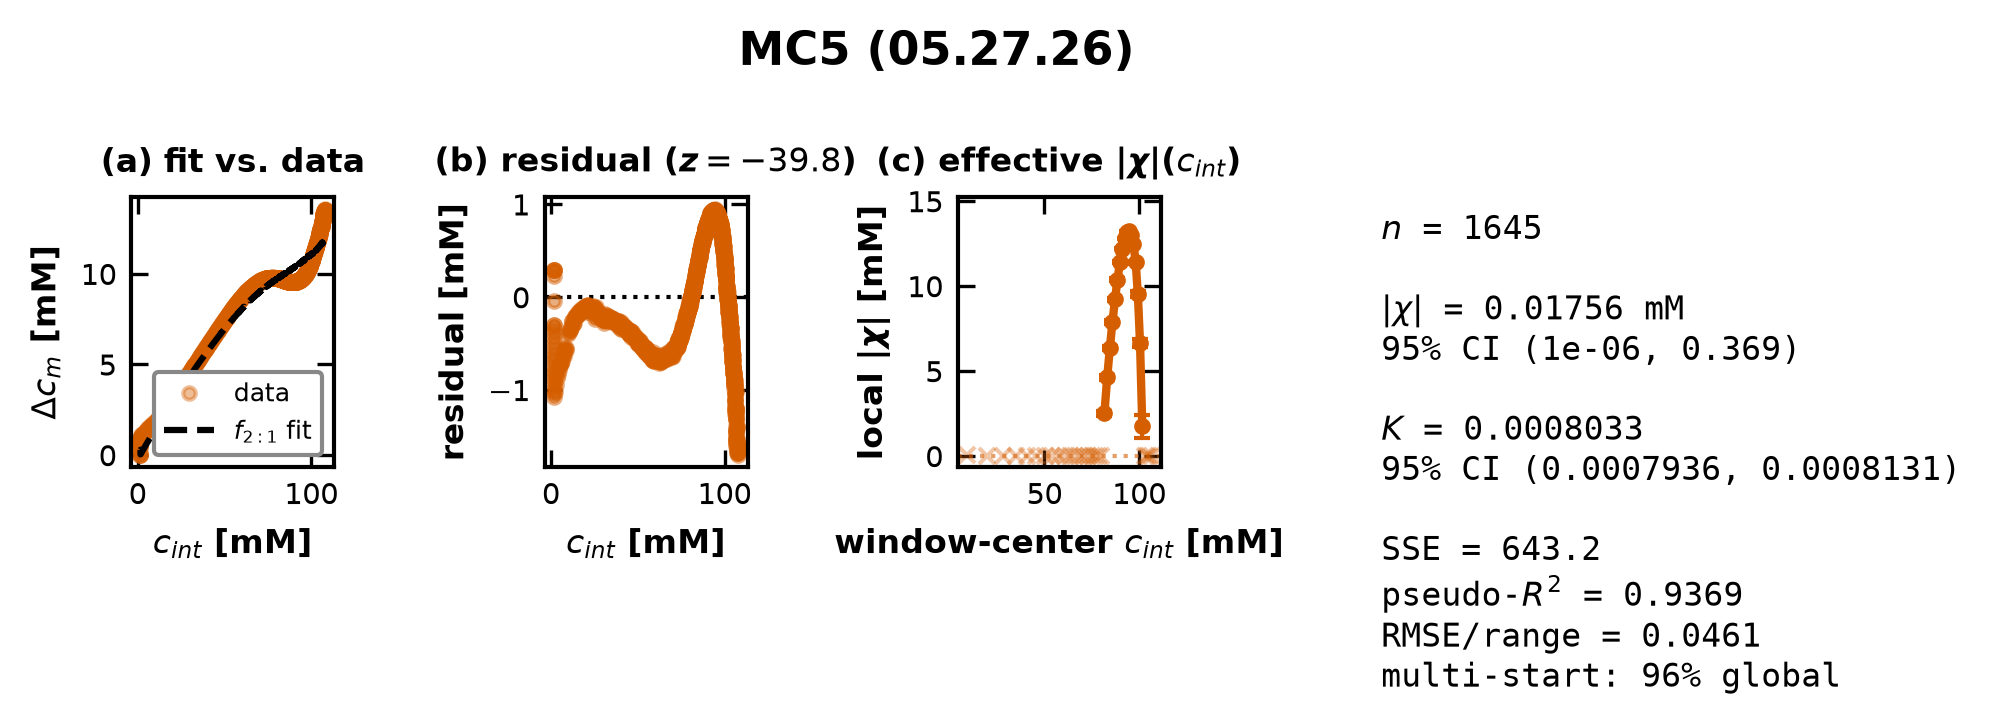
\includegraphics[width=\linewidth]{figures/cacl2_appendix_mc5_0527.png}
\caption{MC5 (05.27.26): fit vs.\ data, residual vs.\ $\cint$, effective
$|\chi|(\cint)$, and parameter summary.}
\end{figure}

\subsection{MC5 (06.27.26)}\label{sec:app-cacl2-mc5b}
$n=1885$, $\cint\in[1.3,103]$\,mM; a near-repeat of MC5 (05.27.26)
(\S\ref{sec:app-cacl2-mc5a}) on the same cut. Bounded fit: $|\chi|=0.0121$
(95\% CI $0$--$0.284$\,mM), $K=0.00032$ (CI $0.00031$--$0.00032$),
$\SSE=1003.8$, pseudo-$R^2=0.838$ (visibly worse than 05.27.26's $0.937$),
99\% multi-start convergence. Residual sign-runs $z=-42.7$. The
effective-$|\chi|$ window fit (21 of 46 reliable) shows the same qualitative
inverted-U shape as 05.27.26 but with a sharper high-$\cint$ drop, mirrored in
panel (a)'s fit-vs-data -- worth a follow-up look at whether this run has more
noise or a genuinely different high-concentration behavior (e.g.\ a different
membrane fouling state on that date; \S\ref{sec:cacl2diag}).
\begin{figure}[H]
\centering
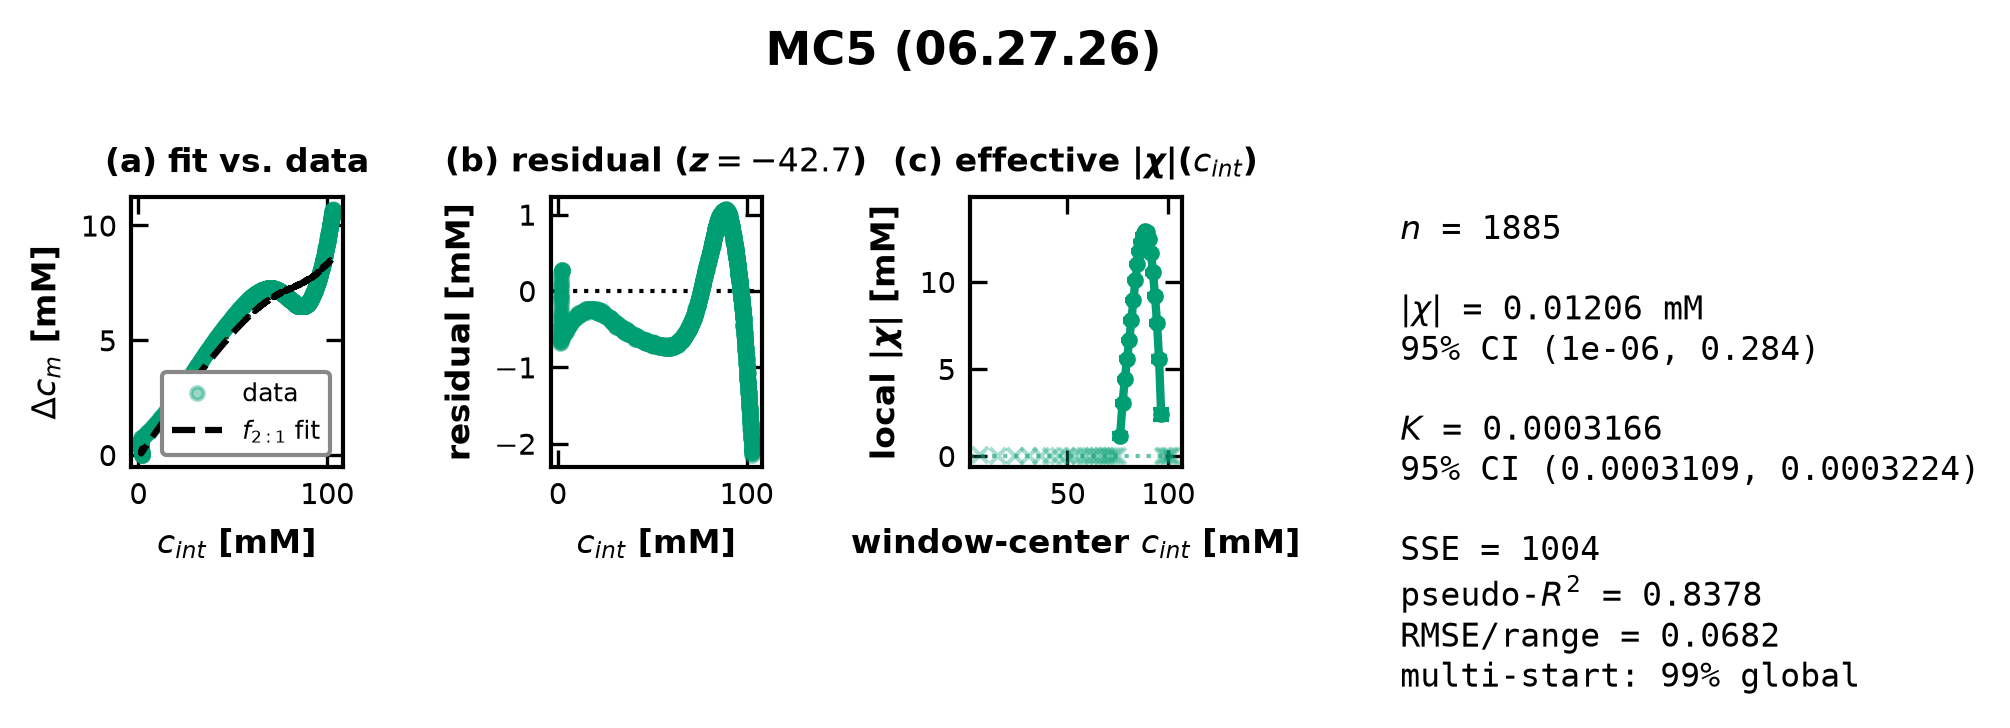
\includegraphics[width=\linewidth]{figures/cacl2_appendix_mc5_0627.png}
\caption{MC5 (06.27.26): fit vs.\ data, residual vs.\ $\cint$, effective
$|\chi|(\cint)$, and parameter summary.}
\end{figure}

% ############################################################
\section{Appendix: Per-Dataset \ce{LaCl3} Detail}\label{sec:lacl3appendix}
% ############################################################
Full fit/residual/drift detail for the single processed \ce{LaCl3} run
summarized in \S\ref{sec:lacl3results}. As with \S\ref{sec:naclappendix}/
\ref{sec:cacl2appendix}, this appendix is a complete reference (favoring
completeness over brevity); read \S\ref{sec:lacl3results}--\ref{sec:lacl3diag}
for the synthesis. The figure shows (a) the corrected-model fit vs.\ data,
(b) the residual vs.\ $\cint$ (with its sign-runs $z$-score), (c) the
sliding-window effective $|\chi|(\cint)$ diagnostic, and (d) the
parameter/CI/fit-quality summary.

\subsection{MC2 (05.21.24)}\label{sec:app-lacl3-mc2}
$n=623$, $\cint\in[2.0,27.8]$\,mM (a narrow range, the same identifiability
headwind flagged for NaCl's MC2 and \ce{CaCl2}'s MC3). Bounded fit:
$|\chi|=0$ (95\% CI $0$--$94.4$\,mM -- pinned at the lower bound), $K=8.758
\times10^{-8}$ (CI $(8.298,\,9.236)\times10^{-8}$), $\SSE=9.677$,
pseudo-$R^2=0.803$, 100\% multi-start convergence. Cross-validated against
Method B (ParmEst nonlinear-constraint quartic, \S\ref{sec:lacl3results}):
$K$ agrees to 5 significant figures, SSE to $<0.01\%$. Residual sign-runs
$z=-24.9$ (strongly non-random, the most extreme of any single-salt dataset
in this report). Of 19 sliding windows, only 7 (all at $\cint\gtrsim
\SI{21}{mM}$) are reliably identified, rising from $\approx0.06$ to
$\approx\SI{0.85}{mM}$ -- \ce{LaCl3}'s effective $|\chi|$ never approaches
even \ce{CaCl2}'s already-small estimates.
\begin{figure}[H]
\centering
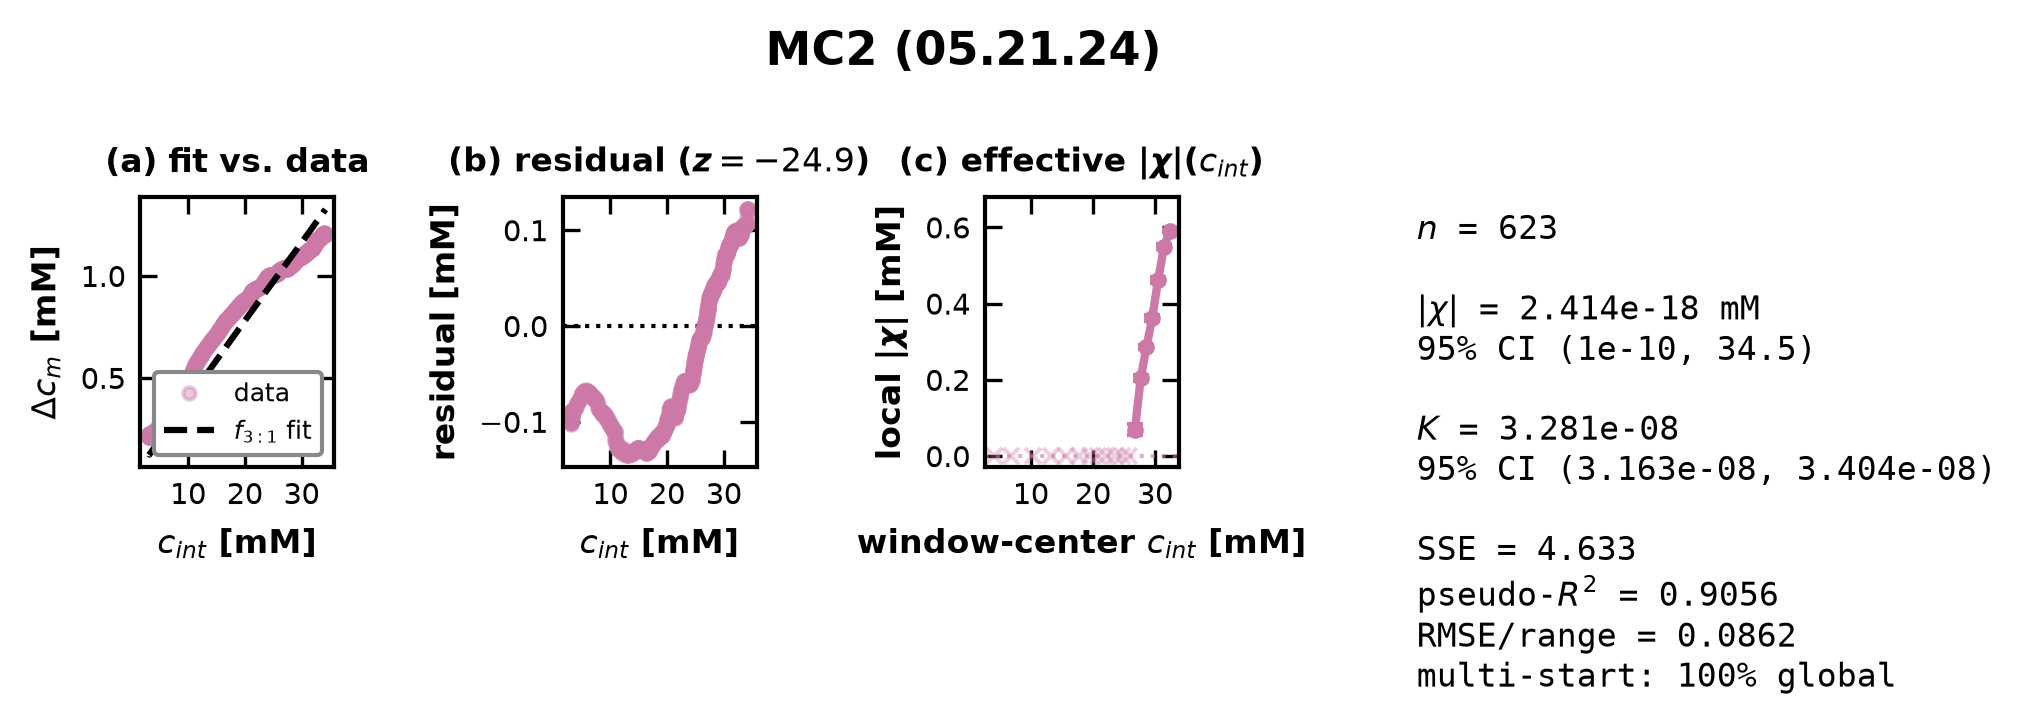
\includegraphics[width=\linewidth]{figures/lacl3_appendix.png}
\caption{MC2 (05.21.24): fit vs.\ data, residual vs.\ $\cint$, effective
$|\chi|(\cint)$, and parameter summary.}
\end{figure}

% ############################################################
\section{Appendix: Per-Dataset Copolymer Detail}\label{sec:copolymerappendix}
% ############################################################
Per-dataset detail for the four copolymer runs summarized in
\S\ref{sec:copolymerresults}--\ref{sec:copolymerdiag}. Unlike
\S\ref{sec:naclappendix}--\ref{sec:lacl3appendix}, this appendix does not
introduce new per-dataset figures -- with only four datasets already shown
individually (by color/panel) in Figures~\ref{fig:copolymerfits},
\ref{fig:copolymerheatmaps}, \ref{fig:copolymerzeta}, \ref{fig:copolymerdiag},
and \ref{fig:copolymerar1}, a further per-dataset figure set would be
redundant; instead each entry below cross-references the relevant panel.

\subsection{PEG0.1-\ce{NaCl}}\label{sec:app-copolymer-peg01nacl}
Raw sheet \texttt{PEG0.1.xlsx / 6.18.24NaCl}, $n=1777$,
$\cint\in[0.62,68.7]$\,mM. Bounded fit: $|\chi|=24.95$ (95\% CI
$8.54$--$232.8$\,mM), $K=0.00195$ (CI $0.00070$--$0.0179$), $\SSE=0.387$,
pseudo-$R^2=0.793$, $58\%$ multi-start convergence. Residual sign-runs
$z=-14.3$ ($n=587$ runs). All 43 sliding windows reliable, local $|\chi|$
rising $20.5\to\SI{199.9}{mM}$ with concentration -- \textbf{drifts},
counter to the non-adsorbing-salt expectation for \ce{Na+}
(\S\ref{sec:copolymerdiag}). Regressed $|\chi|$ is $1.98\times$ the SI
zeta-potential value ($\SI{12.60}{mM}$, PEG0, pH 6.08). AR(1): $\hat\phi=0.999$
($n_{\mathrm{eff}}=0.9/1777$), Wald fold $649\times$ for $|\chi|$. See
Figure~\ref{fig:copolymerfits} (fit), \ref{fig:copolymerdiag} (residual/drift,
blue), \ref{fig:copolymerar1} (AR(1) panel 1), \ref{fig:copolymerzeta} (zeta
comparison), \ref{fig:copolymerheatmaps} (SSE surface, panel 1).

\subsection{PEG6.5-\ce{NaCl}}\label{sec:app-copolymer-peg65nacl}
Raw sheet \texttt{PEG6.5.xlsx / 6.27.24NaCl (2)}, $n=2410$,
$\cint\in[0.03,73.1]$\,mM. Bounded fit: $|\chi|=6148$ (95\% CI $13741$--$550625$\,mM,
\emph{inverted} -- see Table~\ref{tab:copolymerall} caption), $K=0.351$ (CI
$0.761$--$5.41$), $\SSE=0.339$, pseudo-$R^2=0.539$ (the lowest of the four),
$78\%$ multi-start convergence. Residual sign-runs $z=-28.4$ ($n=500$ runs,
the most extreme of the four). \textbf{Weakly identified, not merely
drifting}: 0/59 sliding windows converge reliably, and a direct SSE-profile
check across $|\chi|\in\{0.1,\ldots,50000\}$\,mM shows $<1\%$ SSE change over
a $500\times$ range -- a genuine flat ridge (Figure~\ref{fig:copolymerheatmaps},
panel 2), confirmed not to be an optimizer failure. No SI zeta-potential
$\chi$ exists for PEG6 to validate against. $\phi_{\mathrm w}$ uses PEG4 as a
\emph{proxy} (\S\ref{sec:copolymerimpl}). AR(1): $\hat\phi=0.967$
($n_{\mathrm{eff}}=40.0/2410$, the least severe of the four), Wald fold only
$0.23\times$ -- whitening barely moves an already-uninformative interval.

\subsection{PEG0.1-\ce{Na2SO4}}\label{sec:app-copolymer-peg01na2so4}
Raw sheet \texttt{PEG0.1.xlsx / 8.5.24Na2SO4}, $n=1772$,
$\cint\in[0.07,96.8]$\,mM. Bounded fit (\eqref{eq:na2so4model}):
$|\chi|=1.349$ (95\% CI $1.178$--$1.553$\,mM, well-identified), $K=2.0\times10^{-7}$
(profile-likelihood search returns a degenerate interval at this near-zero
boundary), $\SSE=0.792$, pseudo-$R^2=0.790$, $72\%$ multi-start convergence.
Residual sign-runs $z=-10.3$ ($n=670$ runs -- still non-random, but the
weakest signal of the four). \textbf{The one clean control}: 40/43 reliable
sliding windows, local $|\chi|\in[1.21,1.84]$\,mM with slope $+0.0005$\,mM/mM
-- essentially flat, the expected non-adsorbing-salt signature
(\S\ref{sec:copolymerdiag}). Regressed $|\chi|$ is $0.11\times$ (i.e.\
$\approx9\times$ \emph{lower} than) the SI zeta-potential value for the same
membrane ($\SI{12.60}{mM}$, PEG0) -- the opposite direction of
PEG0.1-\ce{NaCl}'s disagreement, \S\ref{sec:copolymerzeta}. AR(1):
$\hat\phi=0.999$ ($n_{\mathrm{eff}}=0.7/1772$), Wald fold $36\times$.

\subsection{ALK1.2-\ce{Na2SO4}}\label{sec:app-copolymer-alk12na2so4}
Raw sheet \texttt{ALK1.2.xlsx / 5.7.25Na2SO4}, $n=2882$,
$\cint\in[0.03,77.6]$\,mM. \textbf{Calibration derived from the processed
sheet} (\S\ref{sec:copolymerimpl}: this raw sheet has no per-vial
conductivity at all), $R^2=0.9984$, $n=3101$. Bounded fit
(\eqref{eq:na2so4model}): $|\chi|=50.93$ (95\% CI $45.24$--$57.89$\,mM),
$K=0.0176$ (CI $0.0148$--$0.0217$), $\SSE=1870.7$ (the largest of the four --
also the largest $n$ and $\Delta c_{\mathrm m}$ range), pseudo-$R^2=0.763$,
$100\%$ multi-start convergence (the only dataset to fully converge).
Residual sign-runs $z=-9.2$ ($n=1196$ runs). 67/71 reliable sliding windows,
local $|\chi|$ rising $42.9\to\SI{120.9}{mM}$ with concentration --
\textbf{drifts}, despite sharing \ce{Na2SO4}'s co-ion with the clean
PEG0.1-\ce{Na2SO4} case; the drift tracks with membrane identity here, not
salt (\S\ref{sec:copolymerdiag}). No SI zeta-potential $\chi$ exists for
ALK1 to validate against. AR(1): $\hat\phi=0.999$ ($n_{\mathrm{eff}}=0.8/2882$),
Wald fold $69\times$.

\printbibliography

\end{document}
